\documentclass[twoside]{book}

% Packages required by doxygen
\usepackage{calc}
\usepackage{doxygen}
\usepackage{graphicx}
\usepackage[utf8]{inputenc}
\usepackage{makeidx}
\usepackage{multicol}
\usepackage{multirow}
\usepackage{fixltx2e}
\PassOptionsToPackage{warn}{textcomp}
\usepackage{textcomp}
\usepackage[nointegrals]{wasysym}
\usepackage[table]{xcolor}

% Font selection
\usepackage[T1]{fontenc}
\usepackage{mathptmx}
\usepackage[scaled=.90]{helvet}
\usepackage{courier}
\usepackage{amssymb}
\usepackage{sectsty}
\renewcommand{\familydefault}{\sfdefault}
\allsectionsfont{%
  \fontseries{bc}\selectfont%
  \color{darkgray}%
}
\renewcommand{\DoxyLabelFont}{%
  \fontseries{bc}\selectfont%
  \color{darkgray}%
}
\newcommand{\+}{\discretionary{\mbox{\scriptsize$\hookleftarrow$}}{}{}}

% Page & text layout
\usepackage{geometry}
\geometry{%
  a4paper,%
  top=2.5cm,%
  bottom=2.5cm,%
  left=2.5cm,%
  right=2.5cm%
}
\tolerance=750
\hfuzz=15pt
\hbadness=750
\setlength{\emergencystretch}{15pt}
\setlength{\parindent}{0cm}
\setlength{\parskip}{0.2cm}
\makeatletter
\renewcommand{\paragraph}{%
  \@startsection{paragraph}{4}{0ex}{-1.0ex}{1.0ex}{%
    \normalfont\normalsize\bfseries\SS@parafont%
  }%
}
\renewcommand{\subparagraph}{%
  \@startsection{subparagraph}{5}{0ex}{-1.0ex}{1.0ex}{%
    \normalfont\normalsize\bfseries\SS@subparafont%
  }%
}
\makeatother

% Headers & footers
\usepackage{fancyhdr}
\pagestyle{fancyplain}
\fancyhead[LE]{\fancyplain{}{\bfseries\thepage}}
\fancyhead[CE]{\fancyplain{}{}}
\fancyhead[RE]{\fancyplain{}{\bfseries\leftmark}}
\fancyhead[LO]{\fancyplain{}{\bfseries\rightmark}}
\fancyhead[CO]{\fancyplain{}{}}
\fancyhead[RO]{\fancyplain{}{\bfseries\thepage}}
\fancyfoot[LE]{\fancyplain{}{}}
\fancyfoot[CE]{\fancyplain{}{}}
\fancyfoot[RE]{\fancyplain{}{\bfseries\scriptsize Generated on Fri Aug 22 2014 09\+:57\+:17 for Pulsar by Doxygen }}
\fancyfoot[LO]{\fancyplain{}{\bfseries\scriptsize Generated on Fri Aug 22 2014 09\+:57\+:17 for Pulsar by Doxygen }}
\fancyfoot[CO]{\fancyplain{}{}}
\fancyfoot[RO]{\fancyplain{}{}}
\renewcommand{\footrulewidth}{0.4pt}
\renewcommand{\chaptermark}[1]{%
  \markboth{#1}{}%
}
\renewcommand{\sectionmark}[1]{%
  \markright{\thesection\ #1}%
}

% Indices & bibliography
\usepackage{natbib}
\usepackage[titles]{tocloft}
\setcounter{tocdepth}{3}
\setcounter{secnumdepth}{5}
\makeindex

% Hyperlinks (required, but should be loaded last)
\usepackage{ifpdf}
\ifpdf
  \usepackage[pdftex,pagebackref=true]{hyperref}
\else
  \usepackage[ps2pdf,pagebackref=true]{hyperref}
\fi
\hypersetup{%
  colorlinks=true,%
  linkcolor=blue,%
  citecolor=blue,%
  unicode%
}

% Custom commands
\newcommand{\clearemptydoublepage}{%
  \newpage{\pagestyle{empty}\cleardoublepage}%
}


%===== C O N T E N T S =====

\begin{document}

% Titlepage & ToC
\hypersetup{pageanchor=false,
             bookmarks=true,
             bookmarksnumbered=true,
             pdfencoding=unicode
            }
\pagenumbering{roman}
\begin{titlepage}
\vspace*{7cm}
\begin{center}%
{\Large Pulsar }\\
\vspace*{1cm}
{\large Generated by Doxygen 1.8.7}\\
\vspace*{0.5cm}
{\small Fri Aug 22 2014 09:57:17}\\
\end{center}
\end{titlepage}
\clearemptydoublepage
\tableofcontents
\clearemptydoublepage
\pagenumbering{arabic}
\hypersetup{pageanchor=true}

%--- Begin generated contents ---
\chapter{Namespace Index}
\section{Namespace List}
Here is a list of all namespaces with brief descriptions\+:\begin{DoxyCompactList}
\item\contentsline{section}{\hyperlink{namespace_m_h_r}{M\+H\+R} }{\pageref{namespace_m_h_r}}{}
\end{DoxyCompactList}

\chapter{Hierarchical Index}
\section{Class Hierarchy}
This inheritance list is sorted roughly, but not completely, alphabetically\+:\begin{DoxyCompactList}
\item $<$Cv\+Video\+Camera\+Delegate$>$\begin{DoxyCompactList}
\item \contentsline{section}{M\+H\+R\+Main\+View\+Controller}{\pageref{interface_m_h_r_main_view_controller}}{}
\end{DoxyCompactList}
\item \contentsline{section}{M\+H\+R\+:\+:hr\+Debug}{\pageref{struct_m_h_r_1_1hr_debug}}{}
\item \contentsline{section}{M\+H\+R\+:\+:hr\+Result}{\pageref{struct_m_h_r_1_1hr_result}}{}
\item \contentsline{section}{M\+B\+Progress\+H\+U\+D()}{\pageref{category_m_b_progress_h_u_d_07_08}}{}
\item \contentsline{section}{M\+H\+R\+Main\+View\+Controller()}{\pageref{category_m_h_r_main_view_controller_07_08}}{}
\item \contentsline{section}{M\+H\+R\+Result\+View\+Controller()}{\pageref{category_m_h_r_result_view_controller_07_08}}{}
\item \contentsline{section}{M\+H\+R\+Settings\+View\+Controller()}{\pageref{category_m_h_r_settings_view_controller_07_08}}{}
\item N\+S\+Object\begin{DoxyCompactList}
\item \contentsline{section}{M\+H\+R\+Utilities}{\pageref{interface_m_h_r_utilities}}{}
\item \contentsline{section}{U\+I\+Image\+C\+V\+Mat\+Converter}{\pageref{interface_u_i_image_c_v_mat_converter}}{}
\end{DoxyCompactList}
\item $<$N\+S\+Object$>$\begin{DoxyCompactList}
\item \contentsline{section}{$<$M\+H\+R\+Settings\+View\+Delegate$>$}{\pageref{protocol_m_h_r_settings_view_delegate-p}}{}
\begin{DoxyCompactList}
\item \contentsline{section}{M\+H\+R\+Main\+View\+Controller}{\pageref{interface_m_h_r_main_view_controller}}{}
\end{DoxyCompactList}
\end{DoxyCompactList}
\item \contentsline{section}{U\+I\+Alert\+View(Block)}{\pageref{category_u_i_alert_view_07_block_08}}{}
\item $<$U\+I\+Application\+Delegate$>$\begin{DoxyCompactList}
\item \contentsline{section}{M\+H\+R\+App\+Delegate}{\pageref{interface_m_h_r_app_delegate}}{}
\end{DoxyCompactList}
\item U\+I\+Responder\begin{DoxyCompactList}
\item \contentsline{section}{M\+H\+R\+App\+Delegate}{\pageref{interface_m_h_r_app_delegate}}{}
\end{DoxyCompactList}
\item U\+I\+View\begin{DoxyCompactList}
\item \contentsline{section}{M\+B\+Bar\+Progress\+View}{\pageref{interface_m_b_bar_progress_view}}{}
\item \contentsline{section}{M\+B\+Progress\+H\+U\+D}{\pageref{interface_m_b_progress_h_u_d}}{}
\item \contentsline{section}{M\+B\+Round\+Progress\+View}{\pageref{interface_m_b_round_progress_view}}{}
\end{DoxyCompactList}
\item \contentsline{section}{U\+I\+View(Position)}{\pageref{category_u_i_view_07_position_08}}{}
\item U\+I\+View\+Controller\begin{DoxyCompactList}
\item \contentsline{section}{M\+H\+R\+Main\+View\+Controller}{\pageref{interface_m_h_r_main_view_controller}}{}
\item \contentsline{section}{M\+H\+R\+Result\+View\+Controller}{\pageref{interface_m_h_r_result_view_controller}}{}
\item \contentsline{section}{M\+H\+R\+Settings\+View\+Controller}{\pageref{interface_m_h_r_settings_view_controller}}{}
\end{DoxyCompactList}
\item $<$U\+I\+View\+N\+S\+Object$>$\begin{DoxyCompactList}
\item \contentsline{section}{$<$M\+B\+Progress\+H\+U\+D\+Delegate$>$}{\pageref{protocol_m_b_progress_h_u_d_delegate-p}}{}
\end{DoxyCompactList}
\end{DoxyCompactList}

\chapter{Class Index}
\section{Class List}
Here are the classes, structs, unions and interfaces with brief descriptions\+:\begin{DoxyCompactList}
\item\contentsline{section}{\hyperlink{struct_m_h_r_1_1hr_debug}{M\+H\+R\+::hr\+Debug} }{\pageref{struct_m_h_r_1_1hr_debug}}{}
\item\contentsline{section}{\hyperlink{struct_m_h_r_1_1hr_result}{M\+H\+R\+::hr\+Result} }{\pageref{struct_m_h_r_1_1hr_result}}{}
\item\contentsline{section}{\hyperlink{interface_m_b_bar_progress_view}{M\+B\+Bar\+Progress\+View} }{\pageref{interface_m_b_bar_progress_view}}{}
\item\contentsline{section}{\hyperlink{interface_m_b_progress_h_u_d}{M\+B\+Progress\+H\+U\+D} }{\pageref{interface_m_b_progress_h_u_d}}{}
\item\contentsline{section}{\hyperlink{category_m_b_progress_h_u_d_07_08}{M\+B\+Progress\+H\+U\+D()} }{\pageref{category_m_b_progress_h_u_d_07_08}}{}
\item\contentsline{section}{\hyperlink{protocol_m_b_progress_h_u_d_delegate-p}{$<$\+M\+B\+Progress\+H\+U\+D\+Delegate$>$} }{\pageref{protocol_m_b_progress_h_u_d_delegate-p}}{}
\item\contentsline{section}{\hyperlink{interface_m_b_round_progress_view}{M\+B\+Round\+Progress\+View} }{\pageref{interface_m_b_round_progress_view}}{}
\item\contentsline{section}{\hyperlink{interface_m_h_r_app_delegate}{M\+H\+R\+App\+Delegate} }{\pageref{interface_m_h_r_app_delegate}}{}
\item\contentsline{section}{\hyperlink{interface_m_h_r_main_view_controller}{M\+H\+R\+Main\+View\+Controller} }{\pageref{interface_m_h_r_main_view_controller}}{}
\item\contentsline{section}{\hyperlink{category_m_h_r_main_view_controller_07_08}{M\+H\+R\+Main\+View\+Controller()} }{\pageref{category_m_h_r_main_view_controller_07_08}}{}
\item\contentsline{section}{\hyperlink{interface_m_h_r_result_view_controller}{M\+H\+R\+Result\+View\+Controller} }{\pageref{interface_m_h_r_result_view_controller}}{}
\item\contentsline{section}{\hyperlink{category_m_h_r_result_view_controller_07_08}{M\+H\+R\+Result\+View\+Controller()} }{\pageref{category_m_h_r_result_view_controller_07_08}}{}
\item\contentsline{section}{\hyperlink{interface_m_h_r_settings_view_controller}{M\+H\+R\+Settings\+View\+Controller} }{\pageref{interface_m_h_r_settings_view_controller}}{}
\item\contentsline{section}{\hyperlink{category_m_h_r_settings_view_controller_07_08}{M\+H\+R\+Settings\+View\+Controller()} }{\pageref{category_m_h_r_settings_view_controller_07_08}}{}
\item\contentsline{section}{\hyperlink{protocol_m_h_r_settings_view_delegate-p}{$<$\+M\+H\+R\+Settings\+View\+Delegate$>$} }{\pageref{protocol_m_h_r_settings_view_delegate-p}}{}
\item\contentsline{section}{\hyperlink{interface_m_h_r_utilities}{M\+H\+R\+Utilities} }{\pageref{interface_m_h_r_utilities}}{}
\item\contentsline{section}{\hyperlink{category_u_i_alert_view_07_block_08}{U\+I\+Alert\+View(\+Block)} }{\pageref{category_u_i_alert_view_07_block_08}}{}
\item\contentsline{section}{\hyperlink{interface_u_i_image_c_v_mat_converter}{U\+I\+Image\+C\+V\+Mat\+Converter} }{\pageref{interface_u_i_image_c_v_mat_converter}}{}
\item\contentsline{section}{\hyperlink{category_u_i_view_07_position_08}{U\+I\+View(\+Position)} }{\pageref{category_u_i_view_07_position_08}}{}
\end{DoxyCompactList}

\chapter{File Index}
\section{File List}
Here is a list of all files with brief descriptions\+:\begin{DoxyCompactList}
\item\contentsline{section}{\hyperlink{globals_8cpp}{globals.\+cpp} }{\pageref{globals_8cpp}}{}
\item\contentsline{section}{\hyperlink{globals_8h}{globals.\+h} }{\pageref{globals_8h}}{}
\item\contentsline{section}{\hyperlink{main_8m}{main.\+m} }{\pageref{main_8m}}{}
\item\contentsline{section}{\hyperlink{_m_h_r_app_delegate_8hpp}{M\+H\+R\+App\+Delegate.\+hpp} }{\pageref{_m_h_r_app_delegate_8hpp}}{}
\item\contentsline{section}{\hyperlink{_m_h_r_app_delegate_8mm}{M\+H\+R\+App\+Delegate.\+mm} }{\pageref{_m_h_r_app_delegate_8mm}}{}
\item\contentsline{section}{algorithms/\hyperlink{config_8cpp}{config.\+cpp} }{\pageref{config_8cpp}}{}
\item\contentsline{section}{algorithms/\hyperlink{config_8h}{config.\+h} }{\pageref{config_8h}}{}
\item\contentsline{section}{algorithms/\hyperlink{face__params_8h}{face\+\_\+params.\+h} }{\pageref{face__params_8h}}{}
\item\contentsline{section}{algorithms/\hyperlink{finger__params_8h}{finger\+\_\+params.\+h} }{\pageref{finger__params_8h}}{}
\item\contentsline{section}{algorithms/\hyperlink{processing_cumulative_8cpp}{processing\+Cumulative.\+cpp} }{\pageref{processing_cumulative_8cpp}}{}
\item\contentsline{section}{algorithms/\hyperlink{processing_cumulative_8h}{processing\+Cumulative.\+h} }{\pageref{processing_cumulative_8h}}{}
\item\contentsline{section}{algorithms/\hyperlink{processing_per_block_8cpp}{processing\+Per\+Block.\+cpp} }{\pageref{processing_per_block_8cpp}}{}
\item\contentsline{section}{algorithms/\hyperlink{processing_per_block_8h}{processing\+Per\+Block.\+h} }{\pageref{processing_per_block_8h}}{}
\item\contentsline{section}{algorithms/\+Eulerian/\hyperlink{build___gdown__stack_8cpp}{build\+\_\+\+Gdown\+\_\+stack.\+cpp} }{\pageref{build___gdown__stack_8cpp}}{}
\item\contentsline{section}{algorithms/\+Eulerian/\hyperlink{build___gdown__stack_8h}{build\+\_\+\+Gdown\+\_\+stack.\+h} }{\pageref{build___gdown__stack_8h}}{}
\item\contentsline{section}{algorithms/\+Eulerian/\hyperlink{eulerian_8cpp}{eulerian.\+cpp} }{\pageref{eulerian_8cpp}}{}
\item\contentsline{section}{algorithms/\+Eulerian/\hyperlink{eulerian_8h}{eulerian.\+h} }{\pageref{eulerian_8h}}{}
\item\contentsline{section}{algorithms/\+Eulerian/\hyperlink{ideal__bandpassing_8cpp}{ideal\+\_\+bandpassing.\+cpp} }{\pageref{ideal__bandpassing_8cpp}}{}
\item\contentsline{section}{algorithms/\+Eulerian/\hyperlink{ideal__bandpassing_8h}{ideal\+\_\+bandpassing.\+h} }{\pageref{ideal__bandpassing_8h}}{}
\item\contentsline{section}{algorithms/files/\hyperlink{files_8cpp}{files.\+cpp} }{\pageref{files_8cpp}}{}
\item\contentsline{section}{algorithms/files/\hyperlink{files_8h}{files.\+h} }{\pageref{files_8h}}{}
\item\contentsline{section}{algorithms/\+Heart\+Rate\+Cal/\hyperlink{frames2signal_8cpp}{frames2signal.\+cpp} }{\pageref{frames2signal_8cpp}}{}
\item\contentsline{section}{algorithms/\+Heart\+Rate\+Cal/\hyperlink{frames2signal_8h}{frames2signal.\+h} }{\pageref{frames2signal_8h}}{}
\item\contentsline{section}{algorithms/\+Heart\+Rate\+Cal/\hyperlink{hb__counter__autocorr_8cpp}{hb\+\_\+counter\+\_\+autocorr.\+cpp} }{\pageref{hb__counter__autocorr_8cpp}}{}
\item\contentsline{section}{algorithms/\+Heart\+Rate\+Cal/\hyperlink{hb__counter__autocorr_8h}{hb\+\_\+counter\+\_\+autocorr.\+h} }{\pageref{hb__counter__autocorr_8h}}{}
\item\contentsline{section}{algorithms/\+Heart\+Rate\+Cal/\hyperlink{hb__counter__pda_8cpp}{hb\+\_\+counter\+\_\+pda.\+cpp} }{\pageref{hb__counter__pda_8cpp}}{}
\item\contentsline{section}{algorithms/\+Heart\+Rate\+Cal/\hyperlink{hb__counter__pda_8h}{hb\+\_\+counter\+\_\+pda.\+h} }{\pageref{hb__counter__pda_8h}}{}
\item\contentsline{section}{algorithms/\+Heart\+Rate\+Cal/\hyperlink{hr__calculator_8cpp}{hr\+\_\+calculator.\+cpp} }{\pageref{hr__calculator_8cpp}}{}
\item\contentsline{section}{algorithms/\+Heart\+Rate\+Cal/\hyperlink{hr__calculator_8h}{hr\+\_\+calculator.\+h} }{\pageref{hr__calculator_8h}}{}
\item\contentsline{section}{algorithms/\+Heart\+Rate\+Cal/\hyperlink{hr__signal__calc_8cpp}{hr\+\_\+signal\+\_\+calc.\+cpp} }{\pageref{hr__signal__calc_8cpp}}{}
\item\contentsline{section}{algorithms/\+Heart\+Rate\+Cal/\hyperlink{hr__signal__calc_8h}{hr\+\_\+signal\+\_\+calc.\+h} }{\pageref{hr__signal__calc_8h}}{}
\item\contentsline{section}{algorithms/\+Heart\+Rate\+Cal/\hyperlink{hr__structures_8cpp}{hr\+\_\+structures.\+cpp} }{\pageref{hr__structures_8cpp}}{}
\item\contentsline{section}{algorithms/\+Heart\+Rate\+Cal/\hyperlink{hr__structures_8h}{hr\+\_\+structures.\+h} }{\pageref{hr__structures_8h}}{}
\item\contentsline{section}{algorithms/\+Heart\+Rate\+Cal/\hyperlink{temporal__mean__calc_8cpp}{temporal\+\_\+mean\+\_\+calc.\+cpp} }{\pageref{temporal__mean__calc_8cpp}}{}
\item\contentsline{section}{algorithms/\+Heart\+Rate\+Cal/\hyperlink{temporal__mean__calc_8h}{temporal\+\_\+mean\+\_\+calc.\+h} }{\pageref{temporal__mean__calc_8h}}{}
\item\contentsline{section}{algorithms/image/\hyperlink{image_8cpp}{image.\+cpp} }{\pageref{image_8cpp}}{}
\item\contentsline{section}{algorithms/image/\hyperlink{image_8h}{image.\+h} }{\pageref{image_8h}}{}
\item\contentsline{section}{algorithms/math/\hyperlink{matlab_8cpp}{matlab.\+cpp} }{\pageref{matlab_8cpp}}{}
\item\contentsline{section}{algorithms/math/\hyperlink{matlab_8h}{matlab.\+h} }{\pageref{matlab_8h}}{}
\item\contentsline{section}{algorithms/matrix/\hyperlink{matrix_8cpp}{matrix.\+cpp} }{\pageref{matrix_8cpp}}{}
\item\contentsline{section}{algorithms/matrix/\hyperlink{matrix_8h}{matrix.\+h} }{\pageref{matrix_8h}}{}
\item\contentsline{section}{Main\+View/\hyperlink{_m_h_r_main_view_controller_8hpp}{M\+H\+R\+Main\+View\+Controller.\+hpp} }{\pageref{_m_h_r_main_view_controller_8hpp}}{}
\item\contentsline{section}{Main\+View/\hyperlink{_m_h_r_main_view_controller_8mm}{M\+H\+R\+Main\+View\+Controller.\+mm} }{\pageref{_m_h_r_main_view_controller_8mm}}{}
\item\contentsline{section}{Result\+View/\hyperlink{_m_h_r_result_view_controller_8hpp}{M\+H\+R\+Result\+View\+Controller.\+hpp} }{\pageref{_m_h_r_result_view_controller_8hpp}}{}
\item\contentsline{section}{Result\+View/\hyperlink{_m_h_r_result_view_controller_8mm}{M\+H\+R\+Result\+View\+Controller.\+mm} }{\pageref{_m_h_r_result_view_controller_8mm}}{}
\item\contentsline{section}{Settings\+View/\hyperlink{_m_h_r_settings_view_controller_8h}{M\+H\+R\+Settings\+View\+Controller.\+h} }{\pageref{_m_h_r_settings_view_controller_8h}}{}
\item\contentsline{section}{Settings\+View/\hyperlink{_m_h_r_settings_view_controller_8m}{M\+H\+R\+Settings\+View\+Controller.\+m} }{\pageref{_m_h_r_settings_view_controller_8m}}{}
\item\contentsline{section}{Utilities/\hyperlink{auto__start_8hpp}{auto\+\_\+start.\+hpp} }{\pageref{auto__start_8hpp}}{}
\item\contentsline{section}{Utilities/\hyperlink{auto__start_8mm}{auto\+\_\+start.\+mm} }{\pageref{auto__start_8mm}}{}
\item\contentsline{section}{Utilities/\hyperlink{_block_additions_8h}{Block\+Additions.\+h} }{\pageref{_block_additions_8h}}{}
\item\contentsline{section}{Utilities/\hyperlink{_m_b_progress_h_u_d_8h}{M\+B\+Progress\+H\+U\+D.\+h} }{\pageref{_m_b_progress_h_u_d_8h}}{}
\item\contentsline{section}{Utilities/\hyperlink{_m_b_progress_h_u_d_8m}{M\+B\+Progress\+H\+U\+D.\+m} }{\pageref{_m_b_progress_h_u_d_8m}}{}
\item\contentsline{section}{Utilities/\hyperlink{_m_h_r_utilities_8h}{M\+H\+R\+Utilities.\+h} }{\pageref{_m_h_r_utilities_8h}}{}
\item\contentsline{section}{Utilities/\hyperlink{_m_h_r_utilities_8m}{M\+H\+R\+Utilities.\+m} }{\pageref{_m_h_r_utilities_8m}}{}
\item\contentsline{section}{Utilities/\hyperlink{_u_i_alert_view_09_block_8h}{U\+I\+Alert\+View+\+Block.\+h} }{\pageref{_u_i_alert_view_09_block_8h}}{}
\item\contentsline{section}{Utilities/\hyperlink{_u_i_alert_view_09_block_8m}{U\+I\+Alert\+View+\+Block.\+m} }{\pageref{_u_i_alert_view_09_block_8m}}{}
\item\contentsline{section}{Utilities/\hyperlink{_u_i_image_c_v_mat_converter_8hpp}{U\+I\+Image\+C\+V\+Mat\+Converter.\+hpp} }{\pageref{_u_i_image_c_v_mat_converter_8hpp}}{}
\item\contentsline{section}{Utilities/\hyperlink{_u_i_image_c_v_mat_converter_8mm}{U\+I\+Image\+C\+V\+Mat\+Converter.\+mm} }{\pageref{_u_i_image_c_v_mat_converter_8mm}}{}
\item\contentsline{section}{Utilities/\hyperlink{_u_i_view_09_position_8h}{U\+I\+View+\+Position.\+h} }{\pageref{_u_i_view_09_position_8h}}{}
\item\contentsline{section}{Utilities/\hyperlink{_u_i_view_09_position_8m}{U\+I\+View+\+Position.\+m} }{\pageref{_u_i_view_09_position_8m}}{}
\end{DoxyCompactList}

\chapter{Namespace Documentation}
\hypertarget{namespace_m_h_r}{\section{M\+H\+R Namespace Reference}
\label{namespace_m_h_r}\index{M\+H\+R@{M\+H\+R}}
}
\subsection*{Classes}
\begin{DoxyCompactItemize}
\item 
struct \hyperlink{struct_m_h_r_1_1hr_debug}{hr\+Debug}
\item 
struct \hyperlink{struct_m_h_r_1_1hr_result}{hr\+Result}
\end{DoxyCompactItemize}
\subsection*{Functions}
\begin{DoxyCompactItemize}
\item 
void \hyperlink{namespace_m_h_r_a48555f02f08d43ff1f06f9413c86b5ca}{set\+Face\+Params} ()
\item 
void \hyperlink{namespace_m_h_r_af336ca7b239bbe520636c7d147b913b5}{set\+Finger\+Params} ()
\item 
void \hyperlink{namespace_m_h_r_ae1292cc4cfc5411226e0cd77f652e1a5}{build\+\_\+\+Gdown\+\_\+\+Stack} (const vector$<$ Mat $>$ \&vid, vector$<$ Mat $>$ \&G\+Down\+Stack, int start\+Index, int end\+Index, int level)
\item 
void \hyperlink{namespace_m_h_r_af2ec0b4fd5bc225e5e008504e70475a7}{eulerian\+Gaussian\+Pyramid\+Magnification} (const vector$<$ Mat $>$ \&vid, vector$<$ Mat $>$ \&ans, String out\+Dir, double alpha, int level, double freq\+Band\+Low\+End, double freq\+Band\+High\+End, double sampling\+Rate, double chrom\+Attenuation)
\item 
void \hyperlink{namespace_m_h_r_a103bcf8925254f7ca646192777866d4b}{ideal\+\_\+bandpassing} (const vector$<$ Mat $>$ \&src, vector$<$ Mat $>$ \&dst, double wl, double wh, double sampling\+Rate)
\item 
void \hyperlink{namespace_m_h_r_a3b899245a37e41550b80b44fb40fe3e9}{read\+Frame} (const String \&src\+File, vector$<$ Mat $>$ \&dst)
\item 
Mat \hyperlink{namespace_m_h_r_aca720721cf34fb61faddf517a6f1ecb7}{read2\+D\+Mat\+From\+File} (F\+I\+L\+E $\ast$\&file, int rows, int cols)
\item 
vector$<$ double $>$ \hyperlink{namespace_m_h_r_a8b31e05ada67db2ce123a0674568ad29}{read\+Vector\+From\+File} (F\+I\+L\+E $\ast$\&file, int n)
\item 
int \hyperlink{namespace_m_h_r_aca054bab24695d684662a7972fc07d02}{read\+Int} (F\+I\+L\+E $\ast$\&file)
\item 
double \hyperlink{namespace_m_h_r_a30d68a835eaf7530b13d542662a88642}{read\+Double} (F\+I\+L\+E $\ast$\&file)
\item 
void \hyperlink{namespace_m_h_r_a391cd23b86d2d7411411d4595cb74b86}{write\+Vector} (const vector$<$ double $>$ \&src, const String \&out\+File, bool append)
\item 
bool \hyperlink{namespace_m_h_r_aa23b9d8c3b852392335d3d9df6afc874}{frame\+To\+File} (const Mat \&frame, const String \&out\+File)
\item 
void \hyperlink{namespace_m_h_r_a093ff56ed91709ddd3cd6bc1575ca55b}{frame\+Channel\+To\+File} (const Mat \&frame, const String \&out\+File, int channel)
\item 
vector$<$ double $>$ \hyperlink{namespace_m_h_r_a53c0c282e2b27534f2726f735f9664e3}{frames2signal} (const vector$<$ Mat $>$ \&monoframes, const String \&conversion\+\_\+method, double fr, double cutoff\+\_\+freq, double \&lower\+\_\+range, double \&upper\+\_\+range, bool is\+Calc\+Mode)
\item 
vector$<$ int $>$ \hyperlink{namespace_m_h_r_a62a720e54584696fcf7e2d545ad202dc}{hb\+\_\+counter\+\_\+autocorr} (vector$<$ double $>$ \&temporal\+\_\+mean, double fr, int first\+Sample, int window\+\_\+size, double overlap\+\_\+ratio, double min\+Peak\+Distance, \hyperlink{struct_m_h_r_1_1hr_debug}{hr\+Debug} \&debug)
\item 
vector$<$ int $>$ \hyperlink{namespace_m_h_r_ac8cf9fb76b7455034653c17bc9e3ee4c}{hb\+\_\+counter\+\_\+pda} (vector$<$ double $>$ temporal\+\_\+mean, double fr, int first\+Sample, int window\+\_\+size, double overlap\+\_\+ratio, double min\+Peak\+Distance, double threshold, \hyperlink{struct_m_h_r_1_1hr_debug}{hr\+Debug} \&debug)
\item 
void \hyperlink{namespace_m_h_r_a4ba8de262585ae09cd1564fcfda5742e}{hr\+\_\+calculator} (const vector$<$ int $>$ \&heart\+Beat\+Positions, double frame\+Rate, vector$<$ double $>$ \&ans)
\item 
\hyperlink{struct_m_h_r_1_1hr_result}{hr\+Result} \hyperlink{namespace_m_h_r_ac8025fa73e928ab097c9b58525d787b1}{hr\+\_\+signal\+\_\+calc} (vector$<$ double $>$ \&temporal\+\_\+mean, int first\+Sample, int window\+\_\+size, double frame\+Rate, double overlap\+\_\+ratio, double max\+\_\+bpm, double threshold\+\_\+fraction)
\item 
vector$<$ double $>$ \hyperlink{namespace_m_h_r_a6f102a7f405b6c84ea84f4d99e3dd847}{temporal\+\_\+mean\+\_\+calc} (const vector$<$ Mat $>$ \&vid, double overlap\+\_\+ratio, double max\+\_\+bpm, double cutoff\+\_\+freq, int colour\+\_\+channel, String colourspace, double \&lower\+\_\+range, double \&upper\+\_\+range, bool is\+Calc\+Mode)
\item 
void \hyperlink{namespace_m_h_r_ae8dc1afd1e611d432d98186da1f813e5}{rgb2tsl} (const Mat \&rgbmap, Mat \&dst)
\item 
void \hyperlink{namespace_m_h_r_a357c28865a17017a73d0f4ae8c4f7480}{blur\+Dn\+Clr} (const Mat \&src, Mat \&dst, int level)
\item 
void \hyperlink{namespace_m_h_r_a30571de29e1537d20abf69d19329c1bb}{corr\+Dn} (const Mat \&src, Mat \&dst, const Mat \&filter, int rect\+Row, int rect\+Col)
\item 
double \hyperlink{namespace_m_h_r_af6125176deb7b4d4d503a4bcf851a076}{mean} (const vector$<$ double $>$ \&a)
\item 
void \hyperlink{namespace_m_h_r_ad11b22e616f937a6817faa9a0c72ec21}{findpeaks} (const vector$<$ double $>$ \&segment, double min\+Peak\+Distance, double threshold, vector$<$ double $>$ \&max\+\_\+peak\+\_\+strengths, vector$<$ int $>$ \&max\+\_\+peak\+\_\+locs)
\item 
vector$<$ pair$<$ double, int $>$ $>$ \hyperlink{namespace_m_h_r_a22cd3e8872333ff4c203c15821bf69bb}{unique\+\_\+stable} (const vector$<$ pair$<$ double, int $>$$>$ \&arr)
\item 
vector$<$ double $>$ \hyperlink{namespace_m_h_r_a4e7d8efbc84874e131049dc705488cc9}{corr\+\_\+linear} (vector$<$ double $>$ signal, vector$<$ double $>$ kernel, bool subtract\+Mean)
\item 
void \hyperlink{namespace_m_h_r_ab46344d4248f6c55622fef14c1eb78c7}{hist} (const vector$<$ double $>$ \&arr, int nbins, vector$<$ int $>$ \&counts, vector$<$ double $>$ \&centers)
\item 
double \hyperlink{namespace_m_h_r_a4d04157ea7582bbd0a165e1a8a679219}{invprctile} (const vector$<$ double $>$ \&arr, double x)
\item 
double \hyperlink{namespace_m_h_r_a401757908f80823dd6c6ced91e55d751}{prctile} (vector$<$ double $>$ arr, double percent)
\item 
vector$<$ double $>$ \hyperlink{namespace_m_h_r_af85b8b218e683bde30d7ee0329b29716}{low\+\_\+pass\+\_\+filter} (vector$<$ double $>$ arr)
\item 
void \hyperlink{namespace_m_h_r_a0380a36a3a26da3c0a32e0f4b3d9fec9}{gaussian\+Filter} (int length, double sigma, vector$<$ double $>$ \&ans)
\item 
double \hyperlink{namespace_m_h_r_a2e51d3fdfa37bc717ccc0c4557d64445}{diff\+\_\+percent} (double a, double b)
\item 
void \hyperlink{namespace_m_h_r_a8612a874ea7842e4b65969e11f1c2416}{hr\+\_\+polisher} (double \&hr, double \&old\+\_\+hr, double \&hr\+Threshold, double \&hr\+Stan\+Dev)
\item 
Mat \hyperlink{namespace_m_h_r_ad90e260536ab41e3da12f739038743d0}{atan2\+Mat} (const Mat \&a, const Mat \&b)
\item 
Mat \hyperlink{namespace_m_h_r_afef7e1a6e6fe95a9debb07c2d7ba3008}{pow\+Mat} (const Mat \&src, double n)
\item 
Mat \hyperlink{namespace_m_h_r_ac0d7c563ab4072cf5cba2d2b1cb3761e}{add} (const Mat \&a, const Mat \&b)
\item 
Mat \hyperlink{namespace_m_h_r_a497a8cfdabb210ba4d68b592fb589e00}{multiply} (const Mat \&a, const Mat \&b)
\item 
Mat \hyperlink{namespace_m_h_r_a22b0fbac0253b08d84d9c2493324e5db}{multiply} (const Mat \&a, double x)
\item 
void \hyperlink{namespace_m_h_r_a8f470f59589f00a7570d089362d6aa50}{processing\+Cumulative} (vector$<$ double $>$ \&temporal\+\_\+mean, vector$<$ double $>$ temp, \hyperlink{struct_m_h_r_1_1hr_result}{hr\+Result} \&current\+Result)
\item 
void \hyperlink{namespace_m_h_r_af87fd1d23c5d7c0a72caf3061057ebda}{processing\+Per\+Block} (const string \&src\+Dir, const string \&out\+Dir, int file\+Start\+Index, int file\+End\+Index, bool \&is\+Calc\+Mode, double \&lower\+\_\+range, double \&upper\+\_\+range, \hyperlink{struct_m_h_r_1_1hr_result}{hr\+Result} \&result, vector$<$ double $>$ \&tmp)
\end{DoxyCompactItemize}
\subsection*{Variables}
\begin{DoxyCompactItemize}
\item 
int \hyperlink{namespace_m_h_r_a2446951af16ca1137edb21f8e07019cb}{\+\_\+\+D\+E\+B\+U\+G\+\_\+\+M\+O\+D\+E} = 0
\item 
int \hyperlink{namespace_m_h_r_a100c1e31c0fbc8c8b292064c1a8da006}{\+\_\+\+T\+H\+R\+E\+E\+\_\+\+C\+H\+A\+N\+\_\+\+M\+O\+D\+E} = 0
\item 
bool \hyperlink{namespace_m_h_r_a364268cdc7b75db63f89c9d8960aa1b4}{\+\_\+\+F\+A\+C\+E\+\_\+\+M\+O\+D\+E} = true
\item 
String \hyperlink{namespace_m_h_r_a15d81a6b22ae7616409d6df6101690eb}{\+\_\+output\+Path} = \char`\"{}N\+U\+L\+L\char`\"{}
\item 
double \hyperlink{namespace_m_h_r_abbf22419d2dbaf1d661d5b73fc9af29b}{\+\_\+eulerian\+\_\+alpha} = -\/1
\item 
double \hyperlink{namespace_m_h_r_a383bea7ba431fede0a30f05b3ae57536}{\+\_\+eulerian\+\_\+pyr\+Level} = -\/1
\item 
double \hyperlink{namespace_m_h_r_afe8a788bdd0504a98259321e41377180}{\+\_\+eulerian\+\_\+min\+H\+R} = -\/1
\item 
double \hyperlink{namespace_m_h_r_acb647c6b44ad0c7fac0fba37122d5889}{\+\_\+eulerian\+\_\+max\+H\+R} = -\/1
\item 
double \hyperlink{namespace_m_h_r_ab6b7928e4485f421869d4fbac9a5c1cd}{\+\_\+eulerian\+\_\+frame\+Rate} = -\/1
\item 
double \hyperlink{namespace_m_h_r_ad69f0161c9597e078014c52955264fd2}{\+\_\+eulerian\+\_\+chroma\+Magnifier} = -\/1
\item 
int \hyperlink{namespace_m_h_r_a8c0f2199ebe2a27a2fc0cff1daa239ee}{\+\_\+frame\+Rate} = 30
\item 
int \hyperlink{namespace_m_h_r_a2ff626868d0be78114be4abbcd0ba01b}{\+\_\+number\+\_\+of\+\_\+channels} = -\/1
\item 
int \hyperlink{namespace_m_h_r_ac3927bf3a2b93c8dc4ef19ee1a3d55f8}{\+\_\+\+Gpyr\+\_\+filter\+\_\+length} = -\/1
\item 
int \hyperlink{namespace_m_h_r_ad8b548e54d84866330d426d8edc8877e}{\+\_\+start\+Frame} = -\/1
\item 
int \hyperlink{namespace_m_h_r_a08d1602abf6cd2454b1f73a8d5523ac2}{\+\_\+end\+Frame} = -\/1
\item 
double \hyperlink{namespace_m_h_r_a9732a5bb1cbdb99030149ae2bb1cae69}{\+\_\+window\+\_\+size\+\_\+in\+\_\+sec} = -\/1
\item 
double \hyperlink{namespace_m_h_r_aed0501a3045731a781439b11ee82fbfe}{\+\_\+overlap\+\_\+ratio} = -\/1
\item 
double \hyperlink{namespace_m_h_r_a1a13273dd519ccfaf4dc1800bd2031d2}{\+\_\+max\+\_\+bpm} = -\/1
\item 
double \hyperlink{namespace_m_h_r_a9685359cac4522cd1ee584fbfb5371d1}{\+\_\+cutoff\+\_\+freq} = -\/1
\item 
double \hyperlink{namespace_m_h_r_abe9f5a6b09e1219712f2b5912e68506d}{\+\_\+time\+\_\+lag} = -\/1
\item 
String \hyperlink{namespace_m_h_r_a16dd6a785863f2fac97ebb334606c166}{\+\_\+colourspace} = \char`\"{}-\/1\char`\"{}
\item 
int \hyperlink{namespace_m_h_r_a02a81ed541f6536b1632d65c8f2ad0d3}{\+\_\+channels\+\_\+to\+\_\+process} = -\/1
\item 
int \hyperlink{namespace_m_h_r_a5a4548440538bf0354499b42e7983f2f}{\+\_\+number\+\_\+of\+\_\+bins\+\_\+heart\+Rate} = -\/1
\item 
int \hyperlink{namespace_m_h_r_ae2f1f5bafa06074dcb8f0af01a058c81}{\+\_\+flag\+Debug} = -\/1
\item 
int \hyperlink{namespace_m_h_r_ab142c69d1b89170b4fa2533a6f749394}{\+\_\+flag\+Get\+Raw} = -\/1
\item 
int \hyperlink{namespace_m_h_r_a7650c1d1c25787e60c4dbbdb5cedf3b8}{\+\_\+start\+Index} = -\/1
\item 
int \hyperlink{namespace_m_h_r_a43ac6cb857f86cd5a9bc16e968faa1af}{\+\_\+end\+Index} = -\/1
\item 
double \hyperlink{namespace_m_h_r_a8a80b7897b02d4d2a57311a344df8497}{\+\_\+peak\+Strength\+Threshold\+\_\+fraction} = -\/1
\item 
String \hyperlink{namespace_m_h_r_aaaae88f4be078b944fe63b49c5022684}{\+\_\+frames2signal\+Conversion\+Method} = \char`\"{}-\/1\char`\"{}
\item 
int \hyperlink{namespace_m_h_r_a41fcc40bb1f54975292b8d7051b7b3f9}{\+\_\+frame\+\_\+downsampling\+\_\+filt\+\_\+rows} = -\/1
\item 
int \hyperlink{namespace_m_h_r_a619373c68caeeba93f71d9eaeecf1a5b}{\+\_\+frame\+\_\+downsampling\+\_\+filt\+\_\+cols} = -\/1
\item 
Mat \hyperlink{namespace_m_h_r_a8d2bbf36755f538d9b442b415d5cde6d}{\+\_\+frame\+\_\+downsampling\+\_\+filt}
\item 
int \hyperlink{namespace_m_h_r_a87eb7e22893e5160d4a98344bc8bdff4}{\+\_\+trimmed\+\_\+size} = -\/1
\item 
double \hyperlink{namespace_m_h_r_a32705f521f2a65e0b5c5454b328c26db}{\+\_\+training\+\_\+time\+\_\+start} = -\/1
\item 
double \hyperlink{namespace_m_h_r_a6ee9276234c51d213a3b1631eee5f315}{\+\_\+training\+\_\+time\+\_\+end} = -\/1
\item 
int \hyperlink{namespace_m_h_r_ab3a5de59c2eed470e94ca0e79abd2b5c}{\+\_\+number\+\_\+of\+\_\+bins} = -\/1
\item 
double \hyperlink{namespace_m_h_r_acb8b09915d13e40eba7f00718c40ce6a}{\+\_\+pct\+\_\+reach\+\_\+below\+\_\+mode} = -\/1
\item 
double \hyperlink{namespace_m_h_r_a3b2e38d795c8389fd066cefa0af2ef47}{\+\_\+pct\+\_\+reach\+\_\+above\+\_\+mode} = -\/1
\item 
int \hyperlink{namespace_m_h_r_a5d907d8ef896004dce9f0fd1d47b77e7}{\+\_\+beat\+Signal\+Filter\+Kernel\+\_\+size} = -\/1
\item 
Mat \hyperlink{namespace_m_h_r_ab83e011c36b7688dab5ef024c8894300}{\+\_\+beat\+Signal\+Filter\+Kernel}
\item 
double \hyperlink{namespace_m_h_r_ad65f931bf0d5fecacaa5062119d272bf}{\+\_\+hr\+Threshold} = -\/1
\item 
double \hyperlink{namespace_m_h_r_aa202bc96d234c5ee044f8590ad1dc0ef}{\+\_\+hr\+Stan\+Dev} = -\/1
\item 
const double \hyperlink{namespace_m_h_r_a1f2bac57e6ccaebc6afd932278b163ec}{Na\+N} = -\/1e9
\item 
const int \hyperlink{namespace_m_h_r_a167cff7309df5114f9e72af8b5e820c1}{\+\_\+frames\+Block\+\_\+size} = 128
\item 
const int \hyperlink{namespace_m_h_r_aced573ebf5ae641d5c3a58c9762462fb}{\+\_\+min\+Vid\+Length} = 15
\item 
const int \hyperlink{namespace_m_h_r_a0a7cdb59c1f1e8af6e6b61543c81724d}{\+\_\+max\+Vid\+Length} = 30
\item 
const double \hyperlink{namespace_m_h_r_a0f9c0b966020cdd7ef37cb2207d981ab}{\+\_\+face\+\_\+eulerian\+\_\+alpha} = 50
\item 
const double \hyperlink{namespace_m_h_r_a3eae7b41b03bf25902413f62c5e6545d}{\+\_\+face\+\_\+eulerian\+\_\+pyr\+Level} = 6
\item 
const double \hyperlink{namespace_m_h_r_a95e1651df07df85f364ac713aac7a53b}{\+\_\+face\+\_\+eulerian\+\_\+min\+H\+R} = 30
\item 
const double \hyperlink{namespace_m_h_r_a366f66e2cd387cf039dc5d7de4ff5f9d}{\+\_\+face\+\_\+eulerian\+\_\+max\+H\+R} = 240
\item 
const double \hyperlink{namespace_m_h_r_a3c21f6619922e618bff40700a5723015}{\+\_\+face\+\_\+eulerian\+\_\+frame\+Rate} = 30
\item 
const double \hyperlink{namespace_m_h_r_a5b039641e0cf1a30ba4f303e4764b4c8}{\+\_\+face\+\_\+eulerian\+\_\+chroma\+Magnifier} = 1
\item 
const int \hyperlink{namespace_m_h_r_a1af8c23e0ffae759111c964d2369a13b}{\+\_\+face\+\_\+number\+\_\+of\+\_\+channels} = 3
\item 
const int \hyperlink{namespace_m_h_r_a7eabffdab2df22a98e5aa4046d6c3baf}{\+\_\+face\+\_\+\+Gpyr\+\_\+filter\+\_\+length} = 5
\item 
const int \hyperlink{namespace_m_h_r_ac893410fca7e7a76ae562e47f8371cc1}{\+\_\+face\+\_\+start\+Frame} = 0
\item 
const int \hyperlink{namespace_m_h_r_a349e142bd15540a9d0b5b63f426fc3dc}{\+\_\+face\+\_\+end\+Frame} = 0
\item 
const double \hyperlink{namespace_m_h_r_ada7fab40b0e865f6a26751fd550b5288}{\+\_\+face\+\_\+window\+\_\+size\+\_\+in\+\_\+sec} = 10
\item 
const double \hyperlink{namespace_m_h_r_ab6430d316d9d82ce08b7d35fda6ba14e}{\+\_\+face\+\_\+overlap\+\_\+ratio} = 0
\item 
const double \hyperlink{namespace_m_h_r_a123d7bba4eba9d4c49ebe21458394a9a}{\+\_\+face\+\_\+max\+\_\+bpm} = 200
\item 
const double \hyperlink{namespace_m_h_r_afc5d67d6a0c4929f2fc30dce703740fe}{\+\_\+face\+\_\+cutoff\+\_\+freq} = 2.\+5
\item 
const double \hyperlink{namespace_m_h_r_ad108537351ba024dfa150411983a69c4}{\+\_\+face\+\_\+time\+\_\+lag} = 1.\+5
\item 
const String \hyperlink{namespace_m_h_r_a2c3d7c5df37d2106e5f4351ebeb44c2f}{\+\_\+face\+\_\+colourspace} = \char`\"{}tsl\char`\"{}
\item 
const int \hyperlink{namespace_m_h_r_ac3a2dbcaefbcbb5814108c711ebd1fe1}{\+\_\+face\+\_\+channels\+\_\+to\+\_\+process} = 1
\item 
const int \hyperlink{namespace_m_h_r_abfcdcdfbf5694a70c871df5484e30321}{\+\_\+face\+\_\+number\+\_\+of\+\_\+bins\+\_\+heart\+Rate} = 5
\item 
const int \hyperlink{namespace_m_h_r_ade58b99d0d2023434646cb0597baafdf}{\+\_\+face\+\_\+flag\+Debug} = 0
\item 
const int \hyperlink{namespace_m_h_r_a6e9575c56ad75e4e165fd62fad98734f}{\+\_\+face\+\_\+flag\+Get\+Raw} = 0
\item 
const int \hyperlink{namespace_m_h_r_a5c705653d488611b87b11e41e4ffbfd5}{\+\_\+face\+\_\+start\+Index} = 1
\item 
const int \hyperlink{namespace_m_h_r_ad45b2867da1e1b69dee3648585a3ad3a}{\+\_\+face\+\_\+end\+Index} = 0
\item 
const double \hyperlink{namespace_m_h_r_adad3be408f5b45234ee745acc33d6ac8}{\+\_\+face\+\_\+peak\+Strength\+Threshold\+\_\+fraction} = 0
\item 
const String \hyperlink{namespace_m_h_r_a634c25b34e7aa6bbb3cfc346964d2f90}{\+\_\+face\+\_\+frames2signal\+Conversion\+Method} = \char`\"{}mode-\/balance\char`\"{}
\item 
const int \hyperlink{namespace_m_h_r_a7fa6df2df062c81344149450be58164a}{\+\_\+face\+\_\+frame\+\_\+downsampling\+\_\+filt\+\_\+rows} = 7
\item 
const int \hyperlink{namespace_m_h_r_ae762029528d214f277ed064282784d3b}{\+\_\+face\+\_\+frame\+\_\+downsampling\+\_\+filt\+\_\+cols} = 7
\item 
const Mat \hyperlink{namespace_m_h_r_a53c978f9017a65e09546b90474f17111}{\+\_\+face\+\_\+frame\+\_\+downsampling\+\_\+filt}
\item 
const int \hyperlink{namespace_m_h_r_ae64aacd3f078b0c1ecfefee56c27e3ce}{\+\_\+face\+\_\+trimmed\+\_\+size} = 30
\item 
const double \hyperlink{namespace_m_h_r_a4ad71fd0cc039551252ae1929fbbfea9}{\+\_\+face\+\_\+training\+\_\+time\+\_\+start} = 0
\item 
const double \hyperlink{namespace_m_h_r_a86e77ed79df316c170e425d131558571}{\+\_\+face\+\_\+training\+\_\+time\+\_\+end} = 0.\+2
\item 
const int \hyperlink{namespace_m_h_r_a2c4c769eba572cf1388059c68e02804a}{\+\_\+face\+\_\+number\+\_\+of\+\_\+bins} = 50
\item 
const double \hyperlink{namespace_m_h_r_ac4235bc51ec51e261f5822920a5886b0}{\+\_\+face\+\_\+pct\+\_\+reach\+\_\+below\+\_\+mode} = 45
\item 
const double \hyperlink{namespace_m_h_r_a50b60319fb33591915a63ce9b618a18c}{\+\_\+face\+\_\+pct\+\_\+reach\+\_\+above\+\_\+mode} = 45
\item 
const int \hyperlink{namespace_m_h_r_a7f9a1a070d8e2c3eb72d79c71b2f468a}{\+\_\+face\+\_\+beat\+Signal\+Filter\+Kernel\+\_\+size} = 15
\item 
const Mat \hyperlink{namespace_m_h_r_a846528ce2187823d06b73caadf751570}{\+\_\+face\+\_\+beat\+Signal\+Filter\+Kernel}
\item 
const double \hyperlink{namespace_m_h_r_a1e8025b0c611a1a8b4bf74baca52c91c}{\+\_\+face\+\_\+hr\+Threshold} = 40
\item 
const double \hyperlink{namespace_m_h_r_a0eb61186bc00ecb180d50821bee1d360}{\+\_\+face\+\_\+hr\+Stan\+Dev} = 2.\+5
\item 
const int \hyperlink{namespace_m_h_r_adc786b108805d8d2ad944595ea2b7092}{\+\_\+\+T\+H\+R\+E\+S\+H\+O\+L\+D\+\_\+\+N\+O\+\_\+\+F\+A\+C\+E\+\_\+\+F\+R\+A\+M\+E\+S\+\_\+\+M\+I\+N} = 2
\item 
const int \hyperlink{namespace_m_h_r_a90f94ddb83c7c54b9b0836586a51ad43}{\+\_\+\+T\+H\+R\+E\+S\+H\+O\+L\+D\+\_\+\+F\+A\+C\+E\+\_\+\+F\+R\+A\+M\+E\+S\+\_\+\+M\+I\+N} = 2
\item 
const int \hyperlink{namespace_m_h_r_a3c94a936257b6f3257fb7a7768ff4377}{\+\_\+\+T\+H\+R\+E\+S\+H\+O\+L\+D\+\_\+\+F\+A\+C\+E\+\_\+\+F\+R\+A\+M\+E\+S\+\_\+\+F\+O\+R\+\_\+\+S\+T\+A\+R\+T} = 5
\item 
const float \hyperlink{namespace_m_h_r_a4059754ac07ffb5b08e096059f347a82}{\+\_\+\+R\+O\+I\+\_\+\+R\+A\+T\+I\+O\+\_\+\+U\+P\+P\+E\+R} = 1.\+5f
\item 
const float \hyperlink{namespace_m_h_r_a8a54577ca92c7aa81cc87355a7160063}{\+\_\+\+R\+O\+I\+\_\+\+R\+A\+T\+I\+O\+\_\+\+L\+O\+W\+E\+R} = 0.\+8f
\item 
const double \hyperlink{namespace_m_h_r_abe389732cdfc0aa8ebf51a84c4e645a4}{\+\_\+finger\+\_\+eulerian\+\_\+alpha} = 50
\item 
const double \hyperlink{namespace_m_h_r_a197af9978c9b4d443571197f5ad1b019}{\+\_\+finger\+\_\+eulerian\+\_\+pyr\+Level} = 6
\item 
const double \hyperlink{namespace_m_h_r_a2d844de82559885b3d8a333c82b1a733}{\+\_\+finger\+\_\+eulerian\+\_\+min\+H\+R} = 30
\item 
const double \hyperlink{namespace_m_h_r_ab2ef19fc7e685e8a85fbbbc75320fd6e}{\+\_\+finger\+\_\+eulerian\+\_\+max\+H\+R} = 240
\item 
const double \hyperlink{namespace_m_h_r_a6a102813ef2ea5aa11cadcc9ebaa5bbc}{\+\_\+finger\+\_\+eulerian\+\_\+frame\+Rate} = 30
\item 
const double \hyperlink{namespace_m_h_r_adc0b183529468e1b7d2eec8275c004a6}{\+\_\+finger\+\_\+eulerian\+\_\+chroma\+Magnifier} = 1
\item 
const int \hyperlink{namespace_m_h_r_aa01f8308d2cb5cdb00c4a45de8a8cd5e}{\+\_\+finger\+\_\+number\+\_\+of\+\_\+channels} = 3
\item 
const int \hyperlink{namespace_m_h_r_a5b1bf691aa0c1246b140b3f67580c229}{\+\_\+finger\+\_\+\+Gpyr\+\_\+filter\+\_\+length} = 5
\item 
const int \hyperlink{namespace_m_h_r_a9b0e8542961b24a5dc2e1f77df715b51}{\+\_\+finger\+\_\+start\+Frame} = 0
\item 
const int \hyperlink{namespace_m_h_r_aab21e4fd871ccbbdfc656aa4d64aa688}{\+\_\+finger\+\_\+end\+Frame} = 0
\item 
const double \hyperlink{namespace_m_h_r_a04093f94b342ed569322ef2c3a5bcce2}{\+\_\+finger\+\_\+window\+\_\+size\+\_\+in\+\_\+sec} = 10
\item 
const double \hyperlink{namespace_m_h_r_a6ab2b5eaa5246621b9039b65e5501f1c}{\+\_\+finger\+\_\+overlap\+\_\+ratio} = 0
\item 
const double \hyperlink{namespace_m_h_r_ae15a1148a0dba9f30071db8315b9fe88}{\+\_\+finger\+\_\+max\+\_\+bpm} = 200
\item 
const double \hyperlink{namespace_m_h_r_a6125713b446a1bdd5bbc0fb9e75fc58e}{\+\_\+finger\+\_\+cutoff\+\_\+freq} = 2.\+5
\item 
const double \hyperlink{namespace_m_h_r_ae2523999aef7718ac3e6edeb318edf8a}{\+\_\+finger\+\_\+time\+\_\+lag} = 1.\+5
\item 
const String \hyperlink{namespace_m_h_r_af6ec9103edc4e3fe7011676f91c83c26}{\+\_\+finger\+\_\+colourspace} = \char`\"{}rgb\char`\"{}
\item 
const int \hyperlink{namespace_m_h_r_a16934905e88de3a2d084e6734948ec65}{\+\_\+finger\+\_\+channels\+\_\+to\+\_\+process} = 0
\item 
const int \hyperlink{namespace_m_h_r_a2762706b15a5accb61b7efa79cd0617a}{\+\_\+finger\+\_\+number\+\_\+of\+\_\+bins\+\_\+heart\+Rate} = 5
\item 
const int \hyperlink{namespace_m_h_r_aefc7157a4757a4b9017c968a17fb8ee1}{\+\_\+finger\+\_\+flag\+Debug} = 0
\item 
const int \hyperlink{namespace_m_h_r_a24fb7c804c7833388056a5e417354257}{\+\_\+finger\+\_\+flag\+Get\+Raw} = 0
\item 
const int \hyperlink{namespace_m_h_r_a25e5a8e8b0d72f6cfa98fa75e943f35e}{\+\_\+finger\+\_\+start\+Index} = 1
\item 
const int \hyperlink{namespace_m_h_r_a8b1ee45fde805239e5267fb0dcb03735}{\+\_\+finger\+\_\+end\+Index} = 0
\item 
const double \hyperlink{namespace_m_h_r_a417e8c2df65251a5a34b250f975a3867}{\+\_\+finger\+\_\+peak\+Strength\+Threshold\+\_\+fraction} = 0
\item 
const String \hyperlink{namespace_m_h_r_a4c571f87fe52934440add1a3a5a98e14}{\+\_\+finger\+\_\+frames2signal\+Conversion\+Method} = \char`\"{}mode-\/balance\char`\"{}
\item 
const int \hyperlink{namespace_m_h_r_a5d49af784fd77df019705d26d3654953}{\+\_\+finger\+\_\+frame\+\_\+downsampling\+\_\+filt\+\_\+rows} = 7
\item 
const int \hyperlink{namespace_m_h_r_a2c854934355cedc3760bfddd3bcd03a6}{\+\_\+finger\+\_\+frame\+\_\+downsampling\+\_\+filt\+\_\+cols} = 7
\item 
const Mat \hyperlink{namespace_m_h_r_a9a40d6696920c99016b2c4cc40e8db3b}{\+\_\+finger\+\_\+frame\+\_\+downsampling\+\_\+filt}
\item 
const int \hyperlink{namespace_m_h_r_a8a6e23a5b4183588a231061fe7d43524}{\+\_\+finger\+\_\+trimmed\+\_\+size} = 30
\item 
const double \hyperlink{namespace_m_h_r_afcd48923eb1d7b2aff98acc4cf2a9d24}{\+\_\+finger\+\_\+training\+\_\+time\+\_\+start} = 0
\item 
const double \hyperlink{namespace_m_h_r_a69b9408e97af3e5261c4ede559d9f7d6}{\+\_\+finger\+\_\+training\+\_\+time\+\_\+end} = 0.\+2
\item 
const int \hyperlink{namespace_m_h_r_a1cd0eaa85c6115e1d53ad1c1a3209b41}{\+\_\+finger\+\_\+number\+\_\+of\+\_\+bins} = 50
\item 
const double \hyperlink{namespace_m_h_r_a9714df3caf979755314e0a049dd96368}{\+\_\+finger\+\_\+pct\+\_\+reach\+\_\+below\+\_\+mode} = 45
\item 
const double \hyperlink{namespace_m_h_r_a8c272379feda002b512fbc5e3e917000}{\+\_\+finger\+\_\+pct\+\_\+reach\+\_\+above\+\_\+mode} = 45
\item 
const int \hyperlink{namespace_m_h_r_a9b1303d740470ce969352e3173a27ebb}{\+\_\+finger\+\_\+beat\+Signal\+Filter\+Kernel\+\_\+size} = 15
\item 
const Mat \hyperlink{namespace_m_h_r_a7c6f13da1b28c69fdd787e07d05c7503}{\+\_\+finger\+\_\+beat\+Signal\+Filter\+Kernel}
\item 
const double \hyperlink{namespace_m_h_r_ad34bb64ea8d7aec01e0b4a8ae885c2a6}{\+\_\+finger\+\_\+hr\+Threshold} = 40
\item 
const double \hyperlink{namespace_m_h_r_a418b4c21db49ca7ed9f3546cc04f7210}{\+\_\+finger\+\_\+hr\+Stan\+Dev} = 2.\+5
\item 
const Mat \hyperlink{namespace_m_h_r_a7191e886f0a618347db01d5743eb2856}{rgb2ntsc\+\_\+base\+Mat}
\item 
const Mat \hyperlink{namespace_m_h_r_a1ab4a7e6b45362de2827fd373b53ba24}{ntsc2rgb\+\_\+base\+Mat}
\end{DoxyCompactItemize}


\subsection{Function Documentation}
\hypertarget{namespace_m_h_r_ac0d7c563ab4072cf5cba2d2b1cb3761e}{\index{M\+H\+R@{M\+H\+R}!add@{add}}
\index{add@{add}!M\+H\+R@{M\+H\+R}}
\subsubsection[{add}]{\setlength{\rightskip}{0pt plus 5cm}Mat M\+H\+R\+::add (
\begin{DoxyParamCaption}
\item[{const Mat \&}]{a, }
\item[{const Mat \&}]{b}
\end{DoxyParamCaption}
)}}\label{namespace_m_h_r_ac0d7c563ab4072cf5cba2d2b1cb3761e}
\begin{DoxyReturn}{Returns}
a + b 
\end{DoxyReturn}


Definition at line 32 of file matrix.\+cpp.

\hypertarget{namespace_m_h_r_ad90e260536ab41e3da12f739038743d0}{\index{M\+H\+R@{M\+H\+R}!atan2\+Mat@{atan2\+Mat}}
\index{atan2\+Mat@{atan2\+Mat}!M\+H\+R@{M\+H\+R}}
\subsubsection[{atan2\+Mat}]{\setlength{\rightskip}{0pt plus 5cm}Mat M\+H\+R\+::atan2\+Mat (
\begin{DoxyParamCaption}
\item[{const Mat \&}]{a, }
\item[{const Mat \&}]{b}
\end{DoxyParamCaption}
)}}\label{namespace_m_h_r_ad90e260536ab41e3da12f739038743d0}

\begin{DoxyParams}{Parameters}
{\em a,b} & which have the same size ~\newline
\\
\hline
\end{DoxyParams}
\begin{DoxyReturn}{Returns}
a new Mat which each element\mbox{[}i, j\mbox{]} = atan2(a\mbox{[}i, j\mbox{]}, b\mbox{[}i, j\mbox{]}) ~\newline
Data type\+: C\+V\+\_\+64\+F 
\end{DoxyReturn}


Definition at line 13 of file matrix.\+cpp.

\hypertarget{namespace_m_h_r_a357c28865a17017a73d0f4ae8c4f7480}{\index{M\+H\+R@{M\+H\+R}!blur\+Dn\+Clr@{blur\+Dn\+Clr}}
\index{blur\+Dn\+Clr@{blur\+Dn\+Clr}!M\+H\+R@{M\+H\+R}}
\subsubsection[{blur\+Dn\+Clr}]{\setlength{\rightskip}{0pt plus 5cm}void M\+H\+R\+::blur\+Dn\+Clr (
\begin{DoxyParamCaption}
\item[{const Mat \&}]{src, }
\item[{Mat \&}]{dst, }
\item[{int}]{level}
\end{DoxyParamCaption}
)}}\label{namespace_m_h_r_a357c28865a17017a73d0f4ae8c4f7480}
Blur and downsample an image. The blurring is done with filter kernel specified by F\+I\+L\+T (default = 'binom5') ~\newline
 \href{https://github.com/diego898/matlab-utils/blob/master/toolbox/EVM_Matlab/blurDnClr.m}{\tt https\+://github.\+com/diego898/matlab-\/utils/blob/master/toolbox/\+E\+V\+M\+\_\+\+Matlab/blur\+Dn\+Clr.\+m} ~\newline
 \href{http://docs.opencv.org/doc/tutorials/imgproc/pyramids/pyramids.html}{\tt http\+://docs.\+opencv.\+org/doc/tutorials/imgproc/pyramids/pyramids.\+html} ~\newline


Definition at line 89 of file image.\+cpp.

\hypertarget{namespace_m_h_r_ae1292cc4cfc5411226e0cd77f652e1a5}{\index{M\+H\+R@{M\+H\+R}!build\+\_\+\+Gdown\+\_\+\+Stack@{build\+\_\+\+Gdown\+\_\+\+Stack}}
\index{build\+\_\+\+Gdown\+\_\+\+Stack@{build\+\_\+\+Gdown\+\_\+\+Stack}!M\+H\+R@{M\+H\+R}}
\subsubsection[{build\+\_\+\+Gdown\+\_\+\+Stack}]{\setlength{\rightskip}{0pt plus 5cm}void M\+H\+R\+::build\+\_\+\+Gdown\+\_\+\+Stack (
\begin{DoxyParamCaption}
\item[{const vector$<$ Mat $>$ \&}]{vid, }
\item[{vector$<$ Mat $>$ \&}]{G\+Down\+Stack, }
\item[{int}]{start\+Index, }
\item[{int}]{end\+Index, }
\item[{int}]{level}
\end{DoxyParamCaption}
)}}\label{namespace_m_h_r_ae1292cc4cfc5411226e0cd77f652e1a5}
Apply Gaussian pyramid decomposition on {\itshape vid} from {\itshape start\+Index} to {\itshape end\+Index}, and select a specific band indicated by {\itshape level}. ~\newline
\begin{DoxyReturn}{Returns}
{\itshape G\+Down\+Stack} is stack of one band of Gaussian pyramid of each frame 
\end{DoxyReturn}

\begin{DoxyParams}{Parameters}
{\em vid,G\+Down\+Stack} & 
\begin{DoxyItemize}
\item the first dimension is the time axis ~\newline

\item the second dimension is the y axis of the video's frames ~\newline

\item the third dimension is the x axis of the video's frames ~\newline

\item the forth dimension is the color channel ~\newline
Data type\+: C\+V\+\_\+64\+F\+C3 or C\+V\+\_\+64\+F 
\end{DoxyItemize}\\
\hline
\end{DoxyParams}


Definition at line 13 of file build\+\_\+\+Gdown\+\_\+stack.\+cpp.

\hypertarget{namespace_m_h_r_a4e7d8efbc84874e131049dc705488cc9}{\index{M\+H\+R@{M\+H\+R}!corr\+\_\+linear@{corr\+\_\+linear}}
\index{corr\+\_\+linear@{corr\+\_\+linear}!M\+H\+R@{M\+H\+R}}
\subsubsection[{corr\+\_\+linear}]{\setlength{\rightskip}{0pt plus 5cm}vector$<$ double $>$ M\+H\+R\+::corr\+\_\+linear (
\begin{DoxyParamCaption}
\item[{vector$<$ double $>$}]{signal, }
\item[{vector$<$ double $>$}]{kernel, }
\item[{bool}]{subtract\+Mean = {\ttfamily true}}
\end{DoxyParamCaption}
)}}\label{namespace_m_h_r_a4e7d8efbc84874e131049dc705488cc9}
\href{http://www.cs.cornell.edu/courses/CS1114/2013sp/sections/S06_convolution.pdf}{\tt http\+://www.\+cs.\+cornell.\+edu/courses/\+C\+S1114/2013sp/sections/\+S06\+\_\+convolution.\+pdf} \begin{DoxyReturn}{Returns}
1\+D convolution operation of 2 vectors signal and kernel 
\end{DoxyReturn}

\begin{DoxyParams}{Parameters}
{\em subtract\+Mean} & if is true, then before all calculations, each elements of the signal vector will be subtracted by mean({\itshape signal}), and each elements of the kernel vector will be subtracted by mean({\itshape kernel}). \\
\hline
\end{DoxyParams}


Definition at line 87 of file matlab.\+cpp.

\hypertarget{namespace_m_h_r_a30571de29e1537d20abf69d19329c1bb}{\index{M\+H\+R@{M\+H\+R}!corr\+Dn@{corr\+Dn}}
\index{corr\+Dn@{corr\+Dn}!M\+H\+R@{M\+H\+R}}
\subsubsection[{corr\+Dn}]{\setlength{\rightskip}{0pt plus 5cm}void M\+H\+R\+::corr\+Dn (
\begin{DoxyParamCaption}
\item[{const Mat \&}]{src, }
\item[{Mat \&}]{dst, }
\item[{const Mat \&}]{filter, }
\item[{int}]{rect\+Row, }
\item[{int}]{rect\+Col}
\end{DoxyParamCaption}
)}}\label{namespace_m_h_r_a30571de29e1537d20abf69d19329c1bb}
Compute correlation of 2\+D matrices {\itshape src} with {\itshape filter}, followed by downsampling. ~\newline
 \href{http://www.mathworks.com/matlabcentral/fileexchange/43909-separable-steerable-pyramid-toolbox/content/sepspyr/deps/matlabPyrTools-1.3/mpt_corrDn.m}{\tt http\+://www.\+mathworks.\+com/matlabcentral/fileexchange/43909-\/separable-\/steerable-\/pyramid-\/toolbox/content/sepspyr/deps/matlab\+Pyr\+Tools-\/1.\+3/mpt\+\_\+corr\+Dn.\+m} ~\newline
 \href{http://docs.opencv.org/modules/imgproc/doc/filtering.html#void%20filter2D%28InputArray%20src,%20OutputArray%20dst,%20int%20ddepth,%20InputArray%20kernel,%20Point%20anchor,%20double%20delta,%20int%20borderType%29}{\tt http\+://docs.\+opencv.\+org/modules/imgproc/doc/filtering.\+html\#void\%20filter2\+D\%28\+Input\+Array\%20src,\%20\+Output\+Array\%20dst,\%20int\%20ddepth,\%20\+Input\+Array\%20kernel,\%20\+Point\%20anchor,\%20double\%20delta,\%20int\%20border\+Type\%29} ~\newline

\begin{DoxyParams}{Parameters}
{\em src} & must be larger (in both dimensions) than {\itshape filter}. ~\newline
\\
\hline
{\em filter} & is assumed to be floor(size({\itshape filter})/2)+1. ~\newline
\\
\hline
\end{DoxyParams}
\begin{DoxyReturn}{Returns}
{\itshape dst's} data types\+: C\+V\+\_\+64\+F 
\end{DoxyReturn}


Definition at line 99 of file image.\+cpp.

\hypertarget{namespace_m_h_r_a2e51d3fdfa37bc717ccc0c4557d64445}{\index{M\+H\+R@{M\+H\+R}!diff\+\_\+percent@{diff\+\_\+percent}}
\index{diff\+\_\+percent@{diff\+\_\+percent}!M\+H\+R@{M\+H\+R}}
\subsubsection[{diff\+\_\+percent}]{\setlength{\rightskip}{0pt plus 5cm}double M\+H\+R\+::diff\+\_\+percent (
\begin{DoxyParamCaption}
\item[{double}]{a, }
\item[{double}]{b}
\end{DoxyParamCaption}
)}}\label{namespace_m_h_r_a2e51d3fdfa37bc717ccc0c4557d64445}
\begin{DoxyReturn}{Returns}
100$\ast$$\vert$a-\/b$\vert$/b 
\end{DoxyReturn}


Definition at line 234 of file matlab.\+cpp.

\hypertarget{namespace_m_h_r_af2ec0b4fd5bc225e5e008504e70475a7}{\index{M\+H\+R@{M\+H\+R}!eulerian\+Gaussian\+Pyramid\+Magnification@{eulerian\+Gaussian\+Pyramid\+Magnification}}
\index{eulerian\+Gaussian\+Pyramid\+Magnification@{eulerian\+Gaussian\+Pyramid\+Magnification}!M\+H\+R@{M\+H\+R}}
\subsubsection[{eulerian\+Gaussian\+Pyramid\+Magnification}]{\setlength{\rightskip}{0pt plus 5cm}void M\+H\+R\+::eulerian\+Gaussian\+Pyramid\+Magnification (
\begin{DoxyParamCaption}
\item[{const vector$<$ Mat $>$ \&}]{vid, }
\item[{vector$<$ Mat $>$ \&}]{ans, }
\item[{String}]{out\+Dir, }
\item[{double}]{alpha, }
\item[{int}]{level, }
\item[{double}]{freq\+Band\+Low\+End, }
\item[{double}]{freq\+Band\+High\+End, }
\item[{double}]{sampling\+Rate, }
\item[{double}]{chrom\+Attenuation}
\end{DoxyParamCaption}
)}}\label{namespace_m_h_r_af2ec0b4fd5bc225e5e008504e70475a7}
Use Eulerian magnification technique on input frames. ~\newline
Spatial Filtering\+: Gaussian blur and down sample ~\newline
Temporal Filtering\+: Ideal bandpass ~\newline
 \href{http://graphics.cs.cmu.edu/courses/15-463/2012_fall/hw/proj2g-eulerian/}{\tt http\+://graphics.\+cs.\+cmu.\+edu/courses/15-\/463/2012\+\_\+fall/hw/proj2g-\/eulerian/} ~\newline

\begin{DoxyParams}{Parameters}
{\em out\+Dir} & output folder for debug files \\
\hline
{\em alpha} & magnification rate \\
\hline
{\em level} & see \hyperlink{namespace_m_h_r_a357c28865a17017a73d0f4ae8c4f7480}{blur\+Dn\+Clr()} \\
\hline
{\em freq\+Band\+Low\+End} & see {\itshape wl} argument in \hyperlink{namespace_m_h_r_a103bcf8925254f7ca646192777866d4b}{ideal\+\_\+bandpassing()} \\
\hline
{\em freq\+Band\+High\+End} & see {\itshape wh} argument in \hyperlink{namespace_m_h_r_a103bcf8925254f7ca646192777866d4b}{ideal\+\_\+bandpassing()} \\
\hline
{\em sampling\+Rate} & the video's frame rate \\
\hline
{\em chrom\+Attenuation} & the magnification rate of chrom\+A channel in Y\+I\+Q coulourspace \\
\hline
\end{DoxyParams}


Definition at line 13 of file eulerian.\+cpp.

\hypertarget{namespace_m_h_r_ad11b22e616f937a6817faa9a0c72ec21}{\index{M\+H\+R@{M\+H\+R}!findpeaks@{findpeaks}}
\index{findpeaks@{findpeaks}!M\+H\+R@{M\+H\+R}}
\subsubsection[{findpeaks}]{\setlength{\rightskip}{0pt plus 5cm}void M\+H\+R\+::findpeaks (
\begin{DoxyParamCaption}
\item[{const vector$<$ double $>$ \&}]{segment, }
\item[{double}]{min\+Peak\+Distance, }
\item[{double}]{threshold, }
\item[{vector$<$ double $>$ \&}]{max\+\_\+peak\+\_\+strengths, }
\item[{vector$<$ int $>$ \&}]{max\+\_\+peak\+\_\+locs}
\end{DoxyParamCaption}
)}}\label{namespace_m_h_r_ad11b22e616f937a6817faa9a0c72ec21}
findpeaks in {\itshape segment}, with {\itshape min\+Peak\+Distance} and {\itshape threshold},~\newline
complexity O(n$^\wedge$2) with n = number of peaks 
\begin{DoxyParams}{Parameters}
{\em segment} & a vector of signals \\
\hline
{\em min\+Peak\+Distance} & minimum distance between two peaks \\
\hline
{\em threshold} & the minimum value that a peak point should be larger than its two neighbors point \\
\hline
\end{DoxyParams}
\begin{DoxyReturn}{Returns}
{\itshape max\+\_\+peak\+\_\+strengths} 

{\itshape max\+\_\+peak\+\_\+locs} 
\end{DoxyReturn}


Definition at line 24 of file matlab.\+cpp.

\hypertarget{namespace_m_h_r_a093ff56ed91709ddd3cd6bc1575ca55b}{\index{M\+H\+R@{M\+H\+R}!frame\+Channel\+To\+File@{frame\+Channel\+To\+File}}
\index{frame\+Channel\+To\+File@{frame\+Channel\+To\+File}!M\+H\+R@{M\+H\+R}}
\subsubsection[{frame\+Channel\+To\+File}]{\setlength{\rightskip}{0pt plus 5cm}void M\+H\+R\+::frame\+Channel\+To\+File (
\begin{DoxyParamCaption}
\item[{const Mat \&}]{frame, }
\item[{const String \&}]{out\+File, }
\item[{int}]{channel}
\end{DoxyParamCaption}
)}}\label{namespace_m_h_r_a093ff56ed91709ddd3cd6bc1575ca55b}
write a 2\+D Mat to a file as text for the specified {\itshape channel} 

Definition at line 102 of file files.\+cpp.

\hypertarget{namespace_m_h_r_a53c0c282e2b27534f2726f735f9664e3}{\index{M\+H\+R@{M\+H\+R}!frames2signal@{frames2signal}}
\index{frames2signal@{frames2signal}!M\+H\+R@{M\+H\+R}}
\subsubsection[{frames2signal}]{\setlength{\rightskip}{0pt plus 5cm}vector$<$ double $>$ M\+H\+R\+::frames2signal (
\begin{DoxyParamCaption}
\item[{const vector$<$ Mat $>$ \&}]{monoframes, }
\item[{const String \&}]{conversion\+\_\+method, }
\item[{double}]{fr, }
\item[{double}]{cutoff\+\_\+freq, }
\item[{double \&}]{lower\+\_\+range, }
\item[{double \&}]{upper\+\_\+range, }
\item[{bool}]{is\+Calc\+Mode}
\end{DoxyParamCaption}
)}}\label{namespace_m_h_r_a53c0c282e2b27534f2726f735f9664e3}
The function will convert the array of frames into an array of signal value (type double) note that the frame is mono channel. 
\begin{DoxyParams}{Parameters}
{\em fr} & video's frame rate \\
\hline
{\em conversion\+\_\+method} & we have 3 method for converting a frame into a double value\+:
\begin{DoxyItemize}
\item simple-\/mean
\item trimmed-\/mean
\item mode-\/balance 
\end{DoxyItemize}\\
\hline
\end{DoxyParams}
mode \+: 'simple-\/mean' get the mean of all pixel's value in the picture frame

mode \+: 'trimmed-\/mean' get the mean of all pixel's value in a smaller rectangle inside the picture frame

this method will calculate the histogram of pixel's value from the first\+\_\+tranning\+\_\+frames\+\_\+start to first\+\_\+tranning\+\_\+frames\+\_\+end. Then get the bin that has the most number of value, get the centre of that bin as a centre value, then use the prctile function to get the percentile of that centre value. Finally we calculate the mean of values that have the inverted percentile in the range from (centre value's percentile -\/ lower\+\_\+pct\+\_\+range) to (centre value's percentile + upper\+\_\+pct\+\_\+range).

Definition at line 13 of file frames2signal.\+cpp.

\hypertarget{namespace_m_h_r_aa23b9d8c3b852392335d3d9df6afc874}{\index{M\+H\+R@{M\+H\+R}!frame\+To\+File@{frame\+To\+File}}
\index{frame\+To\+File@{frame\+To\+File}!M\+H\+R@{M\+H\+R}}
\subsubsection[{frame\+To\+File}]{\setlength{\rightskip}{0pt plus 5cm}bool M\+H\+R\+::frame\+To\+File (
\begin{DoxyParamCaption}
\item[{const Mat \&}]{frame, }
\item[{const String \&}]{out\+File}
\end{DoxyParamCaption}
)}}\label{namespace_m_h_r_aa23b9d8c3b852392335d3d9df6afc874}
write a 2\+D Mat to an image file 

Definition at line 96 of file files.\+cpp.

\hypertarget{namespace_m_h_r_a0380a36a3a26da3c0a32e0f4b3d9fec9}{\index{M\+H\+R@{M\+H\+R}!gaussian\+Filter@{gaussian\+Filter}}
\index{gaussian\+Filter@{gaussian\+Filter}!M\+H\+R@{M\+H\+R}}
\subsubsection[{gaussian\+Filter}]{\setlength{\rightskip}{0pt plus 5cm}void M\+H\+R\+::gaussian\+Filter (
\begin{DoxyParamCaption}
\item[{int}]{length, }
\item[{double}]{sigma, }
\item[{vector$<$ double $>$ \&}]{ans}
\end{DoxyParamCaption}
)}}\label{namespace_m_h_r_a0380a36a3a26da3c0a32e0f4b3d9fec9}
Generate a vector of Gaussian values of a desired length and properties~\newline
 \href{http://www.mathworks.com/help/images/ref/fspecial.html}{\tt http\+://www.\+mathworks.\+com/help/images/ref/fspecial.\+html} ~\newline
 \href{http://docs.opencv.org/modules/imgproc/doc/filtering.html#Mat%20getGaussianKernel%28int%20ksize,%20double%20sigma,%20int%20ktype%29}{\tt http\+://docs.\+opencv.\+org/modules/imgproc/doc/filtering.\+html\#\+Mat\%20get\+Gaussian\+Kernel\%28int\%20ksize,\%20double\%20sigma,\%20int\%20ktype\%29} ~\newline


Definition at line 222 of file matlab.\+cpp.

\hypertarget{namespace_m_h_r_a62a720e54584696fcf7e2d545ad202dc}{\index{M\+H\+R@{M\+H\+R}!hb\+\_\+counter\+\_\+autocorr@{hb\+\_\+counter\+\_\+autocorr}}
\index{hb\+\_\+counter\+\_\+autocorr@{hb\+\_\+counter\+\_\+autocorr}!M\+H\+R@{M\+H\+R}}
\subsubsection[{hb\+\_\+counter\+\_\+autocorr}]{\setlength{\rightskip}{0pt plus 5cm}vector$<$ int $>$ M\+H\+R\+::hb\+\_\+counter\+\_\+autocorr (
\begin{DoxyParamCaption}
\item[{vector$<$ double $>$ \&}]{temporal\+\_\+mean, }
\item[{double}]{fr, }
\item[{int}]{first\+Sample, }
\item[{int}]{window\+\_\+size, }
\item[{double}]{overlap\+\_\+ratio, }
\item[{double}]{min\+Peak\+Distance, }
\item[{hr\+Debug \&}]{debug}
\end{DoxyParamCaption}
)}}\label{namespace_m_h_r_a62a720e54584696fcf7e2d545ad202dc}
This function will convert the signal array (after using the frame2signal function) to an autocorelation array and then convert to an array of heart beats' position. ~\newline
The function will shift a window with size {\itshape window\+\_\+size} from {\itshape first\+Sample} position to calculate the heart beats in that window. ~\newline
This function is different from the hb\+\_\+counter\+\_\+pda function, instead of calculating the heart beats directly from the signal array, we will first convert the signal array to an autocorrelation array ( \href{http://en.wikipedia.org/wiki/Autocorrelation}{\tt http\+://en.\+wikipedia.\+org/wiki/\+Autocorrelation}) then use this array to calculate the heart beats. ~\newline

\begin{DoxyParams}{Parameters}
{\em fr} & the frame rate. \\
\hline
{\em overlap\+\_\+ratio} & the ratio of the next window will be identical with the current window, at default this ratio value is 0 \\
\hline
{\em min\+Peak\+Distance,threshold} & these arguments are for the find\+Peaks function. \\
\hline
\end{DoxyParams}


Definition at line 13 of file hb\+\_\+counter\+\_\+autocorr.\+cpp.

\hypertarget{namespace_m_h_r_ac8cf9fb76b7455034653c17bc9e3ee4c}{\index{M\+H\+R@{M\+H\+R}!hb\+\_\+counter\+\_\+pda@{hb\+\_\+counter\+\_\+pda}}
\index{hb\+\_\+counter\+\_\+pda@{hb\+\_\+counter\+\_\+pda}!M\+H\+R@{M\+H\+R}}
\subsubsection[{hb\+\_\+counter\+\_\+pda}]{\setlength{\rightskip}{0pt plus 5cm}vector$<$ int $>$ M\+H\+R\+::hb\+\_\+counter\+\_\+pda (
\begin{DoxyParamCaption}
\item[{vector$<$ double $>$}]{temporal\+\_\+mean, }
\item[{double}]{fr, }
\item[{int}]{first\+Sample, }
\item[{int}]{window\+\_\+size, }
\item[{double}]{overlap\+\_\+ratio, }
\item[{double}]{min\+Peak\+Distance, }
\item[{double}]{threshold, }
\item[{hr\+Debug \&}]{debug}
\end{DoxyParamCaption}
)}}\label{namespace_m_h_r_ac8cf9fb76b7455034653c17bc9e3ee4c}
This function will convert the signal array (after using the frame2signal() function) to an array of heart beats' position The function will shift a window with size {\itshape window\+\_\+size} from {\itshape first\+Sample} position to calculate the heart beats in that window. ~\newline

\begin{DoxyParams}{Parameters}
{\em fr} & the frame rate. \\
\hline
{\em overlap\+\_\+ratio} & the ratio of the next window will be identical with the current window, at default this ratio value is 0 \\
\hline
{\em min\+Peak\+Distance,threshold} & these arguments are for the find\+Peaks function. \\
\hline
\end{DoxyParams}


Definition at line 13 of file hb\+\_\+counter\+\_\+pda.\+cpp.

\hypertarget{namespace_m_h_r_ab46344d4248f6c55622fef14c1eb78c7}{\index{M\+H\+R@{M\+H\+R}!hist@{hist}}
\index{hist@{hist}!M\+H\+R@{M\+H\+R}}
\subsubsection[{hist}]{\setlength{\rightskip}{0pt plus 5cm}void M\+H\+R\+::hist (
\begin{DoxyParamCaption}
\item[{const vector$<$ double $>$ \&}]{arr, }
\item[{int}]{nbins, }
\item[{vector$<$ int $>$ \&}]{counts, }
\item[{vector$<$ double $>$ \&}]{centers}
\end{DoxyParamCaption}
)}}\label{namespace_m_h_r_ab46344d4248f6c55622fef14c1eb78c7}
\href{http://www.mathworks.com/help/matlab/ref/hist.html}{\tt http\+://www.\+mathworks.\+com/help/matlab/ref/hist.\+html} \begin{DoxyReturn}{Returns}
{\itshape counts\+:} number of elements in each bin, 

{\itshape centers\+:} the center value of each bin get the histogram of arr's value, the range from min value to max value of the arr will be divided into {\itshape nbins} bins, each bin will have a centres point and a count value denoting number of value in the array belong to that bin's range 
\end{DoxyReturn}


Definition at line 125 of file matlab.\+cpp.

\hypertarget{namespace_m_h_r_a4ba8de262585ae09cd1564fcfda5742e}{\index{M\+H\+R@{M\+H\+R}!hr\+\_\+calculator@{hr\+\_\+calculator}}
\index{hr\+\_\+calculator@{hr\+\_\+calculator}!M\+H\+R@{M\+H\+R}}
\subsubsection[{hr\+\_\+calculator}]{\setlength{\rightskip}{0pt plus 5cm}void M\+H\+R\+::hr\+\_\+calculator (
\begin{DoxyParamCaption}
\item[{const vector$<$ int $>$ \&}]{heart\+Beat\+Positions, }
\item[{double}]{frame\+Rate, }
\item[{vector$<$ double $>$ \&}]{ans}
\end{DoxyParamCaption}
)}}\label{namespace_m_h_r_a4ba8de262585ae09cd1564fcfda5742e}
Calculate the heart-\/rate from a list of heart-\/beat positions. ~\newline

\begin{DoxyParams}{Parameters}
{\em ans} & 
\begin{DoxyItemize}
\item the first number is average heart-\/rate
\item the second number is mode of the instantaneous heart-\/rates multiply with frame\+Rate$\ast$60 
\end{DoxyItemize}\\
\hline
\end{DoxyParams}


Definition at line 14 of file hr\+\_\+calculator.\+cpp.

\hypertarget{namespace_m_h_r_a8612a874ea7842e4b65969e11f1c2416}{\index{M\+H\+R@{M\+H\+R}!hr\+\_\+polisher@{hr\+\_\+polisher}}
\index{hr\+\_\+polisher@{hr\+\_\+polisher}!M\+H\+R@{M\+H\+R}}
\subsubsection[{hr\+\_\+polisher}]{\setlength{\rightskip}{0pt plus 5cm}void M\+H\+R\+::hr\+\_\+polisher (
\begin{DoxyParamCaption}
\item[{double \&}]{hr, }
\item[{double \&}]{old\+\_\+hr, }
\item[{double \&}]{hr\+Threshold, }
\item[{double \&}]{hr\+Stan\+Dev}
\end{DoxyParamCaption}
)}}\label{namespace_m_h_r_a8612a874ea7842e4b65969e11f1c2416}


Definition at line 240 of file matlab.\+cpp.

\hypertarget{namespace_m_h_r_ac8025fa73e928ab097c9b58525d787b1}{\index{M\+H\+R@{M\+H\+R}!hr\+\_\+signal\+\_\+calc@{hr\+\_\+signal\+\_\+calc}}
\index{hr\+\_\+signal\+\_\+calc@{hr\+\_\+signal\+\_\+calc}!M\+H\+R@{M\+H\+R}}
\subsubsection[{hr\+\_\+signal\+\_\+calc}]{\setlength{\rightskip}{0pt plus 5cm}{\bf hr\+Result} M\+H\+R\+::hr\+\_\+signal\+\_\+calc (
\begin{DoxyParamCaption}
\item[{vector$<$ double $>$ \&}]{temporal\+\_\+mean, }
\item[{int}]{first\+Sample, }
\item[{int}]{window\+\_\+size, }
\item[{double}]{frame\+Rate, }
\item[{double}]{overlap\+\_\+ratio, }
\item[{double}]{max\+\_\+bpm, }
\item[{double}]{threshold\+\_\+fraction}
\end{DoxyParamCaption}
)}}\label{namespace_m_h_r_ac8025fa73e928ab097c9b58525d787b1}
Return the average heart-\/rate calculated by autocorr algorithm and pda algorithm. ~\newline

\begin{DoxyParams}{Parameters}
{\em } & see \hyperlink{namespace_m_h_r_ac8cf9fb76b7455034653c17bc9e3ee4c}{hb\+\_\+counter\+\_\+pda()} or \hyperlink{namespace_m_h_r_a62a720e54584696fcf7e2d545ad202dc}{hb\+\_\+counter\+\_\+autocorr()}. \\
\hline
\end{DoxyParams}


Definition at line 13 of file hr\+\_\+signal\+\_\+calc.\+cpp.

\hypertarget{namespace_m_h_r_a103bcf8925254f7ca646192777866d4b}{\index{M\+H\+R@{M\+H\+R}!ideal\+\_\+bandpassing@{ideal\+\_\+bandpassing}}
\index{ideal\+\_\+bandpassing@{ideal\+\_\+bandpassing}!M\+H\+R@{M\+H\+R}}
\subsubsection[{ideal\+\_\+bandpassing}]{\setlength{\rightskip}{0pt plus 5cm}void M\+H\+R\+::ideal\+\_\+bandpassing (
\begin{DoxyParamCaption}
\item[{const vector$<$ Mat $>$ \&}]{src, }
\item[{vector$<$ Mat $>$ \&}]{dst, }
\item[{double}]{wl, }
\item[{double}]{wh, }
\item[{double}]{sampling\+Rate}
\end{DoxyParamCaption}
)}}\label{namespace_m_h_r_a103bcf8925254f7ca646192777866d4b}
Apply ideal band pass filter on {\itshape src}. ~\newline
 \href{http://en.wikipedia.org/wiki/Band-pass_filter}{\tt http\+://en.\+wikipedia.\+org/wiki/\+Band-\/pass\+\_\+filter} 
\begin{DoxyParams}{Parameters}
{\em src,dst} & 
\begin{DoxyItemize}
\item the first dimension is the time axis ~\newline

\item the second dimension is the y axis of the video's frames ~\newline

\item the third dimension is the x axis of the video's frames ~\newline

\item the forth dimension is the color channel ~\newline

\end{DoxyItemize}\\
\hline
{\em wl} & lower cutoff frequency of ideal band pass filter ~\newline
\\
\hline
{\em wh} & higher cutoff frequency of ideal band pass filter ~\newline
\\
\hline
{\em sampling\+Rate} & sampling rate of {\itshape src} ~\newline
Data type\+: C\+V\+\_\+64\+F\+C3 or C\+V\+\_\+64\+F \\
\hline
\end{DoxyParams}


Definition at line 17 of file ideal\+\_\+bandpassing.\+cpp.

\hypertarget{namespace_m_h_r_a4d04157ea7582bbd0a165e1a8a679219}{\index{M\+H\+R@{M\+H\+R}!invprctile@{invprctile}}
\index{invprctile@{invprctile}!M\+H\+R@{M\+H\+R}}
\subsubsection[{invprctile}]{\setlength{\rightskip}{0pt plus 5cm}double M\+H\+R\+::invprctile (
\begin{DoxyParamCaption}
\item[{const vector$<$ double $>$ \&}]{arr, }
\item[{double}]{x}
\end{DoxyParamCaption}
)}}\label{namespace_m_h_r_a4d04157ea7582bbd0a165e1a8a679219}
get the invert percentile of arr with value x. \begin{DoxyReturn}{Returns}
the percent of number of values in arr that smaller or equal x. 
\end{DoxyReturn}


Definition at line 164 of file matlab.\+cpp.

\hypertarget{namespace_m_h_r_af85b8b218e683bde30d7ee0329b29716}{\index{M\+H\+R@{M\+H\+R}!low\+\_\+pass\+\_\+filter@{low\+\_\+pass\+\_\+filter}}
\index{low\+\_\+pass\+\_\+filter@{low\+\_\+pass\+\_\+filter}!M\+H\+R@{M\+H\+R}}
\subsubsection[{low\+\_\+pass\+\_\+filter}]{\setlength{\rightskip}{0pt plus 5cm}vector$<$ double $>$ M\+H\+R\+::low\+\_\+pass\+\_\+filter (
\begin{DoxyParamCaption}
\item[{vector$<$ double $>$}]{arr}
\end{DoxyParamCaption}
)}}\label{namespace_m_h_r_af85b8b218e683bde30d7ee0329b29716}
filter function for frames2signal function, apply low pass filter on vector {\itshape arr}.  \href{http://en.wikipedia.org/wiki/Low-pass_filter}{\tt http\+://en.\+wikipedia.\+org/wiki/\+Low-\/pass\+\_\+filter} 

Definition at line 194 of file matlab.\+cpp.

\hypertarget{namespace_m_h_r_af6125176deb7b4d4d503a4bcf851a076}{\index{M\+H\+R@{M\+H\+R}!mean@{mean}}
\index{mean@{mean}!M\+H\+R@{M\+H\+R}}
\subsubsection[{mean}]{\setlength{\rightskip}{0pt plus 5cm}double M\+H\+R\+::mean (
\begin{DoxyParamCaption}
\item[{const vector$<$ double $>$ \&}]{a}
\end{DoxyParamCaption}
)}}\label{namespace_m_h_r_af6125176deb7b4d4d503a4bcf851a076}
\begin{DoxyReturn}{Returns}
the mean value of a double vector 
\end{DoxyReturn}


Definition at line 14 of file matlab.\+cpp.

\hypertarget{namespace_m_h_r_a497a8cfdabb210ba4d68b592fb589e00}{\index{M\+H\+R@{M\+H\+R}!multiply@{multiply}}
\index{multiply@{multiply}!M\+H\+R@{M\+H\+R}}
\subsubsection[{multiply}]{\setlength{\rightskip}{0pt plus 5cm}Mat M\+H\+R\+::multiply (
\begin{DoxyParamCaption}
\item[{const Mat \&}]{a, }
\item[{const Mat \&}]{b}
\end{DoxyParamCaption}
)}}\label{namespace_m_h_r_a497a8cfdabb210ba4d68b592fb589e00}
\begin{DoxyReturn}{Returns}
a $\ast$ b (element-\/wise) 
\end{DoxyReturn}


Definition at line 40 of file matrix.\+cpp.

\hypertarget{namespace_m_h_r_a22b0fbac0253b08d84d9c2493324e5db}{\index{M\+H\+R@{M\+H\+R}!multiply@{multiply}}
\index{multiply@{multiply}!M\+H\+R@{M\+H\+R}}
\subsubsection[{multiply}]{\setlength{\rightskip}{0pt plus 5cm}Mat M\+H\+R\+::multiply (
\begin{DoxyParamCaption}
\item[{const Mat \&}]{a, }
\item[{double}]{x}
\end{DoxyParamCaption}
)}}\label{namespace_m_h_r_a22b0fbac0253b08d84d9c2493324e5db}
\begin{DoxyReturn}{Returns}
a new Mat which each element\mbox{[}i, j\mbox{]} = a\mbox{[}i, j\mbox{]} $\ast$ x ~\newline
Data type\+: C\+V\+\_\+64\+F 
\end{DoxyReturn}


Definition at line 48 of file matrix.\+cpp.

\hypertarget{namespace_m_h_r_afef7e1a6e6fe95a9debb07c2d7ba3008}{\index{M\+H\+R@{M\+H\+R}!pow\+Mat@{pow\+Mat}}
\index{pow\+Mat@{pow\+Mat}!M\+H\+R@{M\+H\+R}}
\subsubsection[{pow\+Mat}]{\setlength{\rightskip}{0pt plus 5cm}Mat M\+H\+R\+::pow\+Mat (
\begin{DoxyParamCaption}
\item[{const Mat \&}]{src, }
\item[{double}]{n}
\end{DoxyParamCaption}
)}}\label{namespace_m_h_r_afef7e1a6e6fe95a9debb07c2d7ba3008}
\begin{DoxyReturn}{Returns}
the {\itshape n-\/th} power of {\itshape src} (element-\/wise) ~\newline
Data type\+: C\+V\+\_\+64\+F 
\end{DoxyReturn}


Definition at line 24 of file matrix.\+cpp.

\hypertarget{namespace_m_h_r_a401757908f80823dd6c6ced91e55d751}{\index{M\+H\+R@{M\+H\+R}!prctile@{prctile}}
\index{prctile@{prctile}!M\+H\+R@{M\+H\+R}}
\subsubsection[{prctile}]{\setlength{\rightskip}{0pt plus 5cm}double M\+H\+R\+::prctile (
\begin{DoxyParamCaption}
\item[{vector$<$ double $>$}]{arr, }
\item[{double}]{percent}
\end{DoxyParamCaption}
)}}\label{namespace_m_h_r_a401757908f80823dd6c6ced91e55d751}
get the percentile of arr with a percent value. 

Definition at line 172 of file matlab.\+cpp.

\hypertarget{namespace_m_h_r_a8f470f59589f00a7570d089362d6aa50}{\index{M\+H\+R@{M\+H\+R}!processing\+Cumulative@{processing\+Cumulative}}
\index{processing\+Cumulative@{processing\+Cumulative}!M\+H\+R@{M\+H\+R}}
\subsubsection[{processing\+Cumulative}]{\setlength{\rightskip}{0pt plus 5cm}void M\+H\+R\+::processing\+Cumulative (
\begin{DoxyParamCaption}
\item[{vector$<$ double $>$ \&}]{temporal\+\_\+mean, }
\item[{vector$<$ double $>$}]{temp, }
\item[{hr\+Result \&}]{current\+Result}
\end{DoxyParamCaption}
)}}\label{namespace_m_h_r_a8f470f59589f00a7570d089362d6aa50}


Definition at line 13 of file processing\+Cumulative.\+cpp.

\hypertarget{namespace_m_h_r_af87fd1d23c5d7c0a72caf3061057ebda}{\index{M\+H\+R@{M\+H\+R}!processing\+Per\+Block@{processing\+Per\+Block}}
\index{processing\+Per\+Block@{processing\+Per\+Block}!M\+H\+R@{M\+H\+R}}
\subsubsection[{processing\+Per\+Block}]{\setlength{\rightskip}{0pt plus 5cm}void M\+H\+R\+::processing\+Per\+Block (
\begin{DoxyParamCaption}
\item[{const string \&}]{src\+Dir, }
\item[{const string \&}]{out\+Dir, }
\item[{int}]{file\+Start\+Index, }
\item[{int}]{file\+End\+Index, }
\item[{bool \&}]{is\+Calc\+Mode, }
\item[{double \&}]{lower\+\_\+range, }
\item[{double \&}]{upper\+\_\+range, }
\item[{hr\+Result \&}]{result, }
\item[{vector$<$ double $>$ \&}]{tmp}
\end{DoxyParamCaption}
)}}\label{namespace_m_h_r_af87fd1d23c5d7c0a72caf3061057ebda}


Definition at line 12 of file processing\+Per\+Block.\+cpp.

\hypertarget{namespace_m_h_r_aca720721cf34fb61faddf517a6f1ecb7}{\index{M\+H\+R@{M\+H\+R}!read2\+D\+Mat\+From\+File@{read2\+D\+Mat\+From\+File}}
\index{read2\+D\+Mat\+From\+File@{read2\+D\+Mat\+From\+File}!M\+H\+R@{M\+H\+R}}
\subsubsection[{read2\+D\+Mat\+From\+File}]{\setlength{\rightskip}{0pt plus 5cm}Mat M\+H\+R\+::read2\+D\+Mat\+From\+File (
\begin{DoxyParamCaption}
\item[{F\+I\+L\+E $\ast$\&}]{file, }
\item[{int}]{rows, }
\item[{int}]{cols}
\end{DoxyParamCaption}
)}}\label{namespace_m_h_r_aca720721cf34fb61faddf517a6f1ecb7}
read a 2\+D Mat ({\itshape rows} $\ast$ {\itshape cols}) from an opened file 

Definition at line 39 of file files.\+cpp.

\hypertarget{namespace_m_h_r_a30d68a835eaf7530b13d542662a88642}{\index{M\+H\+R@{M\+H\+R}!read\+Double@{read\+Double}}
\index{read\+Double@{read\+Double}!M\+H\+R@{M\+H\+R}}
\subsubsection[{read\+Double}]{\setlength{\rightskip}{0pt plus 5cm}double M\+H\+R\+::read\+Double (
\begin{DoxyParamCaption}
\item[{F\+I\+L\+E $\ast$\&}]{file}
\end{DoxyParamCaption}
)}}\label{namespace_m_h_r_a30d68a835eaf7530b13d542662a88642}
read a double number from an opened file 

Definition at line 69 of file files.\+cpp.

\hypertarget{namespace_m_h_r_a3b899245a37e41550b80b44fb40fe3e9}{\index{M\+H\+R@{M\+H\+R}!read\+Frame@{read\+Frame}}
\index{read\+Frame@{read\+Frame}!M\+H\+R@{M\+H\+R}}
\subsubsection[{read\+Frame}]{\setlength{\rightskip}{0pt plus 5cm}void M\+H\+R\+::read\+Frame (
\begin{DoxyParamCaption}
\item[{const String \&}]{src\+File, }
\item[{vector$<$ Mat $>$ \&}]{dst}
\end{DoxyParamCaption}
)}}\label{namespace_m_h_r_a3b899245a37e41550b80b44fb40fe3e9}
read frames from a file to a a Mat vector 

Definition at line 13 of file files.\+cpp.

\hypertarget{namespace_m_h_r_aca054bab24695d684662a7972fc07d02}{\index{M\+H\+R@{M\+H\+R}!read\+Int@{read\+Int}}
\index{read\+Int@{read\+Int}!M\+H\+R@{M\+H\+R}}
\subsubsection[{read\+Int}]{\setlength{\rightskip}{0pt plus 5cm}int M\+H\+R\+::read\+Int (
\begin{DoxyParamCaption}
\item[{F\+I\+L\+E $\ast$\&}]{file}
\end{DoxyParamCaption}
)}}\label{namespace_m_h_r_aca054bab24695d684662a7972fc07d02}
read an integer from an opened file 

Definition at line 61 of file files.\+cpp.

\hypertarget{namespace_m_h_r_a8b31e05ada67db2ce123a0674568ad29}{\index{M\+H\+R@{M\+H\+R}!read\+Vector\+From\+File@{read\+Vector\+From\+File}}
\index{read\+Vector\+From\+File@{read\+Vector\+From\+File}!M\+H\+R@{M\+H\+R}}
\subsubsection[{read\+Vector\+From\+File}]{\setlength{\rightskip}{0pt plus 5cm}vector$<$ double $>$ M\+H\+R\+::read\+Vector\+From\+File (
\begin{DoxyParamCaption}
\item[{F\+I\+L\+E $\ast$\&}]{file, }
\item[{int}]{n}
\end{DoxyParamCaption}
)}}\label{namespace_m_h_r_a8b31e05ada67db2ce123a0674568ad29}
read a vector$<$double$>$ with {\itshape n} elements from an opened file 

Definition at line 49 of file files.\+cpp.

\hypertarget{namespace_m_h_r_ae8dc1afd1e611d432d98186da1f813e5}{\index{M\+H\+R@{M\+H\+R}!rgb2tsl@{rgb2tsl}}
\index{rgb2tsl@{rgb2tsl}!M\+H\+R@{M\+H\+R}}
\subsubsection[{rgb2tsl}]{\setlength{\rightskip}{0pt plus 5cm}void M\+H\+R\+::rgb2tsl (
\begin{DoxyParamCaption}
\item[{const Mat \&}]{rgbmap, }
\item[{Mat \&}]{dst}
\end{DoxyParamCaption}
)}}\label{namespace_m_h_r_ae8dc1afd1e611d432d98186da1f813e5}
convert a R\+G\+B frame to a T\+S\+L frame ~\newline
Data type\+: C\+V\+\_\+64\+F\+C3 ~\newline
 \href{http://en.wikipedia.org/wiki/TSL_color_space}{\tt http\+://en.\+wikipedia.\+org/wiki/\+T\+S\+L\+\_\+color\+\_\+space} 

Definition at line 12 of file image.\+cpp.

\hypertarget{namespace_m_h_r_a48555f02f08d43ff1f06f9413c86b5ca}{\index{M\+H\+R@{M\+H\+R}!set\+Face\+Params@{set\+Face\+Params}}
\index{set\+Face\+Params@{set\+Face\+Params}!M\+H\+R@{M\+H\+R}}
\subsubsection[{set\+Face\+Params}]{\setlength{\rightskip}{0pt plus 5cm}void M\+H\+R\+::set\+Face\+Params (
\begin{DoxyParamCaption}
{}
\end{DoxyParamCaption}
)}}\label{namespace_m_h_r_a48555f02f08d43ff1f06f9413c86b5ca}


Definition at line 84 of file config.\+cpp.

\hypertarget{namespace_m_h_r_af336ca7b239bbe520636c7d147b913b5}{\index{M\+H\+R@{M\+H\+R}!set\+Finger\+Params@{set\+Finger\+Params}}
\index{set\+Finger\+Params@{set\+Finger\+Params}!M\+H\+R@{M\+H\+R}}
\subsubsection[{set\+Finger\+Params}]{\setlength{\rightskip}{0pt plus 5cm}void M\+H\+R\+::set\+Finger\+Params (
\begin{DoxyParamCaption}
{}
\end{DoxyParamCaption}
)}}\label{namespace_m_h_r_af336ca7b239bbe520636c7d147b913b5}


Definition at line 139 of file config.\+cpp.

\hypertarget{namespace_m_h_r_a6f102a7f405b6c84ea84f4d99e3dd847}{\index{M\+H\+R@{M\+H\+R}!temporal\+\_\+mean\+\_\+calc@{temporal\+\_\+mean\+\_\+calc}}
\index{temporal\+\_\+mean\+\_\+calc@{temporal\+\_\+mean\+\_\+calc}!M\+H\+R@{M\+H\+R}}
\subsubsection[{temporal\+\_\+mean\+\_\+calc}]{\setlength{\rightskip}{0pt plus 5cm}vector$<$ double $>$ M\+H\+R\+::temporal\+\_\+mean\+\_\+calc (
\begin{DoxyParamCaption}
\item[{const vector$<$ Mat $>$ \&}]{vid, }
\item[{double}]{overlap\+\_\+ratio, }
\item[{double}]{max\+\_\+bpm, }
\item[{double}]{cutoff\+\_\+freq, }
\item[{int}]{colour\+\_\+channel, }
\item[{String}]{colourspace, }
\item[{double \&}]{lower\+\_\+range, }
\item[{double \&}]{upper\+\_\+range, }
\item[{bool}]{is\+Calc\+Mode}
\end{DoxyParamCaption}
)}}\label{namespace_m_h_r_a6f102a7f405b6c84ea84f4d99e3dd847}
Convert frames of $<$vid$>$ to signals. 
\begin{DoxyParams}{Parameters}
{\em vid} & data type is C\+V\+\_\+64\+F\+C3 or C\+V\+\_\+64\+F \\
\hline
{\em overlap\+\_\+ratio} & overlap ratio between 2 consecutive segments \\
\hline
{\em max\+\_\+bpm} & maximum heart rate detectable (use in determining min\+Peaks\+Distance in \hyperlink{namespace_m_h_r_ad11b22e616f937a6817faa9a0c72ec21}{findpeaks()}) \\
\hline
{\em colour\+\_\+channel} & if in \+\_\+\+T\+H\+R\+E\+E\+\_\+\+C\+H\+A\+N\+\_\+\+M\+O\+D\+E, then convert all frames of {\itshape vid} to monoframes by select only one channel of each frame. \\
\hline
{\em colourspace} & if in \+\_\+\+T\+H\+R\+E\+E\+\_\+\+C\+H\+A\+N\+\_\+\+M\+O\+D\+E, then convert colourspace of all frames of {\itshape vid} to \char`\"{}hsv\char`\"{}, \char`\"{}ycbcr\char`\"{} or \char`\"{}tsl\char`\"{} before converting them to monoframes \\
\hline
{\em cutoff\+\_\+freq,lower\+\_\+range,upper\+\_\+range$>$,is\+Calc\+Mode} & see \hyperlink{namespace_m_h_r_a53c0c282e2b27534f2726f735f9664e3}{frames2signal()} \\
\hline
\end{DoxyParams}


Definition at line 13 of file temporal\+\_\+mean\+\_\+calc.\+cpp.

\hypertarget{namespace_m_h_r_a22cd3e8872333ff4c203c15821bf69bb}{\index{M\+H\+R@{M\+H\+R}!unique\+\_\+stable@{unique\+\_\+stable}}
\index{unique\+\_\+stable@{unique\+\_\+stable}!M\+H\+R@{M\+H\+R}}
\subsubsection[{unique\+\_\+stable}]{\setlength{\rightskip}{0pt plus 5cm}vector$<$ pair$<$ double, int $>$ $>$ M\+H\+R\+::unique\+\_\+stable (
\begin{DoxyParamCaption}
\item[{const vector$<$ pair$<$ double, int $>$$>$ \&}]{arr}
\end{DoxyParamCaption}
)}}\label{namespace_m_h_r_a22cd3e8872333ff4c203c15821bf69bb}
remove all identical item in the arr, two items are equal if the second value (type int) of them are equal.~\newline
all identical item will be removed just left the first appearing value.~\newline
the order will be reserve. 

Definition at line 74 of file matlab.\+cpp.

\hypertarget{namespace_m_h_r_a391cd23b86d2d7411411d4595cb74b86}{\index{M\+H\+R@{M\+H\+R}!write\+Vector@{write\+Vector}}
\index{write\+Vector@{write\+Vector}!M\+H\+R@{M\+H\+R}}
\subsubsection[{write\+Vector}]{\setlength{\rightskip}{0pt plus 5cm}void M\+H\+R\+::write\+Vector (
\begin{DoxyParamCaption}
\item[{const vector$<$ double $>$ \&}]{src, }
\item[{const String \&}]{out\+File, }
\item[{bool}]{append = {\ttfamily false}}
\end{DoxyParamCaption}
)}}\label{namespace_m_h_r_a391cd23b86d2d7411411d4595cb74b86}
write a vector$<$double$>$ to a file. ~\newline

\begin{DoxyParams}{Parameters}
{\em append} & if == true, then the function will append the vector at the end of the file, otherwise, it will overwrite the old file or create a new file \\
\hline
\end{DoxyParams}


Definition at line 77 of file files.\+cpp.



\subsection{Variable Documentation}
\hypertarget{namespace_m_h_r_ab83e011c36b7688dab5ef024c8894300}{\index{M\+H\+R@{M\+H\+R}!\+\_\+beat\+Signal\+Filter\+Kernel@{\+\_\+beat\+Signal\+Filter\+Kernel}}
\index{\+\_\+beat\+Signal\+Filter\+Kernel@{\+\_\+beat\+Signal\+Filter\+Kernel}!M\+H\+R@{M\+H\+R}}
\subsubsection[{\+\_\+beat\+Signal\+Filter\+Kernel}]{\setlength{\rightskip}{0pt plus 5cm}Mat M\+H\+R\+::\+\_\+beat\+Signal\+Filter\+Kernel}}\label{namespace_m_h_r_ab83e011c36b7688dab5ef024c8894300}


Definition at line 76 of file config.\+cpp.

\hypertarget{namespace_m_h_r_a5d907d8ef896004dce9f0fd1d47b77e7}{\index{M\+H\+R@{M\+H\+R}!\+\_\+beat\+Signal\+Filter\+Kernel\+\_\+size@{\+\_\+beat\+Signal\+Filter\+Kernel\+\_\+size}}
\index{\+\_\+beat\+Signal\+Filter\+Kernel\+\_\+size@{\+\_\+beat\+Signal\+Filter\+Kernel\+\_\+size}!M\+H\+R@{M\+H\+R}}
\subsubsection[{\+\_\+beat\+Signal\+Filter\+Kernel\+\_\+size}]{\setlength{\rightskip}{0pt plus 5cm}int M\+H\+R\+::\+\_\+beat\+Signal\+Filter\+Kernel\+\_\+size = -\/1}}\label{namespace_m_h_r_a5d907d8ef896004dce9f0fd1d47b77e7}


Definition at line 75 of file config.\+cpp.

\hypertarget{namespace_m_h_r_a02a81ed541f6536b1632d65c8f2ad0d3}{\index{M\+H\+R@{M\+H\+R}!\+\_\+channels\+\_\+to\+\_\+process@{\+\_\+channels\+\_\+to\+\_\+process}}
\index{\+\_\+channels\+\_\+to\+\_\+process@{\+\_\+channels\+\_\+to\+\_\+process}!M\+H\+R@{M\+H\+R}}
\subsubsection[{\+\_\+channels\+\_\+to\+\_\+process}]{\setlength{\rightskip}{0pt plus 5cm}int M\+H\+R\+::\+\_\+channels\+\_\+to\+\_\+process = -\/1}}\label{namespace_m_h_r_a02a81ed541f6536b1632d65c8f2ad0d3}


Definition at line 42 of file config.\+cpp.

\hypertarget{namespace_m_h_r_a16dd6a785863f2fac97ebb334606c166}{\index{M\+H\+R@{M\+H\+R}!\+\_\+colourspace@{\+\_\+colourspace}}
\index{\+\_\+colourspace@{\+\_\+colourspace}!M\+H\+R@{M\+H\+R}}
\subsubsection[{\+\_\+colourspace}]{\setlength{\rightskip}{0pt plus 5cm}String M\+H\+R\+::\+\_\+colourspace = \char`\"{}-\/1\char`\"{}}}\label{namespace_m_h_r_a16dd6a785863f2fac97ebb334606c166}


Definition at line 41 of file config.\+cpp.

\hypertarget{namespace_m_h_r_a9685359cac4522cd1ee584fbfb5371d1}{\index{M\+H\+R@{M\+H\+R}!\+\_\+cutoff\+\_\+freq@{\+\_\+cutoff\+\_\+freq}}
\index{\+\_\+cutoff\+\_\+freq@{\+\_\+cutoff\+\_\+freq}!M\+H\+R@{M\+H\+R}}
\subsubsection[{\+\_\+cutoff\+\_\+freq}]{\setlength{\rightskip}{0pt plus 5cm}double M\+H\+R\+::\+\_\+cutoff\+\_\+freq = -\/1}}\label{namespace_m_h_r_a9685359cac4522cd1ee584fbfb5371d1}


Definition at line 39 of file config.\+cpp.

\hypertarget{namespace_m_h_r_a2446951af16ca1137edb21f8e07019cb}{\index{M\+H\+R@{M\+H\+R}!\+\_\+\+D\+E\+B\+U\+G\+\_\+\+M\+O\+D\+E@{\+\_\+\+D\+E\+B\+U\+G\+\_\+\+M\+O\+D\+E}}
\index{\+\_\+\+D\+E\+B\+U\+G\+\_\+\+M\+O\+D\+E@{\+\_\+\+D\+E\+B\+U\+G\+\_\+\+M\+O\+D\+E}!M\+H\+R@{M\+H\+R}}
\subsubsection[{\+\_\+\+D\+E\+B\+U\+G\+\_\+\+M\+O\+D\+E}]{\setlength{\rightskip}{0pt plus 5cm}int M\+H\+R\+::\+\_\+\+D\+E\+B\+U\+G\+\_\+\+M\+O\+D\+E = 0}}\label{namespace_m_h_r_a2446951af16ca1137edb21f8e07019cb}


Definition at line 13 of file config.\+cpp.

\hypertarget{namespace_m_h_r_a08d1602abf6cd2454b1f73a8d5523ac2}{\index{M\+H\+R@{M\+H\+R}!\+\_\+end\+Frame@{\+\_\+end\+Frame}}
\index{\+\_\+end\+Frame@{\+\_\+end\+Frame}!M\+H\+R@{M\+H\+R}}
\subsubsection[{\+\_\+end\+Frame}]{\setlength{\rightskip}{0pt plus 5cm}int M\+H\+R\+::\+\_\+end\+Frame = -\/1}}\label{namespace_m_h_r_a08d1602abf6cd2454b1f73a8d5523ac2}


Definition at line 33 of file config.\+cpp.

\hypertarget{namespace_m_h_r_a43ac6cb857f86cd5a9bc16e968faa1af}{\index{M\+H\+R@{M\+H\+R}!\+\_\+end\+Index@{\+\_\+end\+Index}}
\index{\+\_\+end\+Index@{\+\_\+end\+Index}!M\+H\+R@{M\+H\+R}}
\subsubsection[{\+\_\+end\+Index}]{\setlength{\rightskip}{0pt plus 5cm}int M\+H\+R\+::\+\_\+end\+Index = -\/1}}\label{namespace_m_h_r_a43ac6cb857f86cd5a9bc16e968faa1af}


Definition at line 50 of file config.\+cpp.

\hypertarget{namespace_m_h_r_abbf22419d2dbaf1d661d5b73fc9af29b}{\index{M\+H\+R@{M\+H\+R}!\+\_\+eulerian\+\_\+alpha@{\+\_\+eulerian\+\_\+alpha}}
\index{\+\_\+eulerian\+\_\+alpha@{\+\_\+eulerian\+\_\+alpha}!M\+H\+R@{M\+H\+R}}
\subsubsection[{\+\_\+eulerian\+\_\+alpha}]{\setlength{\rightskip}{0pt plus 5cm}double M\+H\+R\+::\+\_\+eulerian\+\_\+alpha = -\/1}}\label{namespace_m_h_r_abbf22419d2dbaf1d661d5b73fc9af29b}


Definition at line 21 of file config.\+cpp.

\hypertarget{namespace_m_h_r_ad69f0161c9597e078014c52955264fd2}{\index{M\+H\+R@{M\+H\+R}!\+\_\+eulerian\+\_\+chroma\+Magnifier@{\+\_\+eulerian\+\_\+chroma\+Magnifier}}
\index{\+\_\+eulerian\+\_\+chroma\+Magnifier@{\+\_\+eulerian\+\_\+chroma\+Magnifier}!M\+H\+R@{M\+H\+R}}
\subsubsection[{\+\_\+eulerian\+\_\+chroma\+Magnifier}]{\setlength{\rightskip}{0pt plus 5cm}double M\+H\+R\+::\+\_\+eulerian\+\_\+chroma\+Magnifier = -\/1}}\label{namespace_m_h_r_ad69f0161c9597e078014c52955264fd2}


Definition at line 26 of file config.\+cpp.

\hypertarget{namespace_m_h_r_ab6b7928e4485f421869d4fbac9a5c1cd}{\index{M\+H\+R@{M\+H\+R}!\+\_\+eulerian\+\_\+frame\+Rate@{\+\_\+eulerian\+\_\+frame\+Rate}}
\index{\+\_\+eulerian\+\_\+frame\+Rate@{\+\_\+eulerian\+\_\+frame\+Rate}!M\+H\+R@{M\+H\+R}}
\subsubsection[{\+\_\+eulerian\+\_\+frame\+Rate}]{\setlength{\rightskip}{0pt plus 5cm}double M\+H\+R\+::\+\_\+eulerian\+\_\+frame\+Rate = -\/1}}\label{namespace_m_h_r_ab6b7928e4485f421869d4fbac9a5c1cd}


Definition at line 25 of file config.\+cpp.

\hypertarget{namespace_m_h_r_acb647c6b44ad0c7fac0fba37122d5889}{\index{M\+H\+R@{M\+H\+R}!\+\_\+eulerian\+\_\+max\+H\+R@{\+\_\+eulerian\+\_\+max\+H\+R}}
\index{\+\_\+eulerian\+\_\+max\+H\+R@{\+\_\+eulerian\+\_\+max\+H\+R}!M\+H\+R@{M\+H\+R}}
\subsubsection[{\+\_\+eulerian\+\_\+max\+H\+R}]{\setlength{\rightskip}{0pt plus 5cm}double M\+H\+R\+::\+\_\+eulerian\+\_\+max\+H\+R = -\/1}}\label{namespace_m_h_r_acb647c6b44ad0c7fac0fba37122d5889}


Definition at line 24 of file config.\+cpp.

\hypertarget{namespace_m_h_r_afe8a788bdd0504a98259321e41377180}{\index{M\+H\+R@{M\+H\+R}!\+\_\+eulerian\+\_\+min\+H\+R@{\+\_\+eulerian\+\_\+min\+H\+R}}
\index{\+\_\+eulerian\+\_\+min\+H\+R@{\+\_\+eulerian\+\_\+min\+H\+R}!M\+H\+R@{M\+H\+R}}
\subsubsection[{\+\_\+eulerian\+\_\+min\+H\+R}]{\setlength{\rightskip}{0pt plus 5cm}double M\+H\+R\+::\+\_\+eulerian\+\_\+min\+H\+R = -\/1}}\label{namespace_m_h_r_afe8a788bdd0504a98259321e41377180}


Definition at line 23 of file config.\+cpp.

\hypertarget{namespace_m_h_r_a383bea7ba431fede0a30f05b3ae57536}{\index{M\+H\+R@{M\+H\+R}!\+\_\+eulerian\+\_\+pyr\+Level@{\+\_\+eulerian\+\_\+pyr\+Level}}
\index{\+\_\+eulerian\+\_\+pyr\+Level@{\+\_\+eulerian\+\_\+pyr\+Level}!M\+H\+R@{M\+H\+R}}
\subsubsection[{\+\_\+eulerian\+\_\+pyr\+Level}]{\setlength{\rightskip}{0pt plus 5cm}double M\+H\+R\+::\+\_\+eulerian\+\_\+pyr\+Level = -\/1}}\label{namespace_m_h_r_a383bea7ba431fede0a30f05b3ae57536}


Definition at line 22 of file config.\+cpp.

\hypertarget{namespace_m_h_r_a846528ce2187823d06b73caadf751570}{\index{M\+H\+R@{M\+H\+R}!\+\_\+face\+\_\+beat\+Signal\+Filter\+Kernel@{\+\_\+face\+\_\+beat\+Signal\+Filter\+Kernel}}
\index{\+\_\+face\+\_\+beat\+Signal\+Filter\+Kernel@{\+\_\+face\+\_\+beat\+Signal\+Filter\+Kernel}!M\+H\+R@{M\+H\+R}}
\subsubsection[{\+\_\+face\+\_\+beat\+Signal\+Filter\+Kernel}]{\setlength{\rightskip}{0pt plus 5cm}const Mat M\+H\+R\+::\+\_\+face\+\_\+beat\+Signal\+Filter\+Kernel}}\label{namespace_m_h_r_a846528ce2187823d06b73caadf751570}
{\bfseries Initial value\+:}
\begin{DoxyCode}
= (Mat\_<double>(1, \hyperlink{namespace_m_h_r_a7f9a1a070d8e2c3eb72d79c71b2f468a}{\_face\_beatSignalFilterKernel\_size}) <<
                                              -0.0265, -0.0076, 0.0217, 0.0580, 0.0956,
                                              0.1285, 0.1509, 0.1589, 0.1509, 0.1285,
                                              0.0956, 0.0580, 0.0217, -0.0076, -0.0265)
\end{DoxyCode}


Definition at line 82 of file face\+\_\+params.\+h.

\hypertarget{namespace_m_h_r_a7f9a1a070d8e2c3eb72d79c71b2f468a}{\index{M\+H\+R@{M\+H\+R}!\+\_\+face\+\_\+beat\+Signal\+Filter\+Kernel\+\_\+size@{\+\_\+face\+\_\+beat\+Signal\+Filter\+Kernel\+\_\+size}}
\index{\+\_\+face\+\_\+beat\+Signal\+Filter\+Kernel\+\_\+size@{\+\_\+face\+\_\+beat\+Signal\+Filter\+Kernel\+\_\+size}!M\+H\+R@{M\+H\+R}}
\subsubsection[{\+\_\+face\+\_\+beat\+Signal\+Filter\+Kernel\+\_\+size}]{\setlength{\rightskip}{0pt plus 5cm}const int M\+H\+R\+::\+\_\+face\+\_\+beat\+Signal\+Filter\+Kernel\+\_\+size = 15}}\label{namespace_m_h_r_a7f9a1a070d8e2c3eb72d79c71b2f468a}


Definition at line 81 of file face\+\_\+params.\+h.

\hypertarget{namespace_m_h_r_ac3a2dbcaefbcbb5814108c711ebd1fe1}{\index{M\+H\+R@{M\+H\+R}!\+\_\+face\+\_\+channels\+\_\+to\+\_\+process@{\+\_\+face\+\_\+channels\+\_\+to\+\_\+process}}
\index{\+\_\+face\+\_\+channels\+\_\+to\+\_\+process@{\+\_\+face\+\_\+channels\+\_\+to\+\_\+process}!M\+H\+R@{M\+H\+R}}
\subsubsection[{\+\_\+face\+\_\+channels\+\_\+to\+\_\+process}]{\setlength{\rightskip}{0pt plus 5cm}const int M\+H\+R\+::\+\_\+face\+\_\+channels\+\_\+to\+\_\+process = 1}}\label{namespace_m_h_r_ac3a2dbcaefbcbb5814108c711ebd1fe1}


Definition at line 40 of file face\+\_\+params.\+h.

\hypertarget{namespace_m_h_r_a2c3d7c5df37d2106e5f4351ebeb44c2f}{\index{M\+H\+R@{M\+H\+R}!\+\_\+face\+\_\+colourspace@{\+\_\+face\+\_\+colourspace}}
\index{\+\_\+face\+\_\+colourspace@{\+\_\+face\+\_\+colourspace}!M\+H\+R@{M\+H\+R}}
\subsubsection[{\+\_\+face\+\_\+colourspace}]{\setlength{\rightskip}{0pt plus 5cm}const String M\+H\+R\+::\+\_\+face\+\_\+colourspace = \char`\"{}tsl\char`\"{}}}\label{namespace_m_h_r_a2c3d7c5df37d2106e5f4351ebeb44c2f}


Definition at line 39 of file face\+\_\+params.\+h.

\hypertarget{namespace_m_h_r_afc5d67d6a0c4929f2fc30dce703740fe}{\index{M\+H\+R@{M\+H\+R}!\+\_\+face\+\_\+cutoff\+\_\+freq@{\+\_\+face\+\_\+cutoff\+\_\+freq}}
\index{\+\_\+face\+\_\+cutoff\+\_\+freq@{\+\_\+face\+\_\+cutoff\+\_\+freq}!M\+H\+R@{M\+H\+R}}
\subsubsection[{\+\_\+face\+\_\+cutoff\+\_\+freq}]{\setlength{\rightskip}{0pt plus 5cm}const double M\+H\+R\+::\+\_\+face\+\_\+cutoff\+\_\+freq = 2.\+5}}\label{namespace_m_h_r_afc5d67d6a0c4929f2fc30dce703740fe}


Definition at line 37 of file face\+\_\+params.\+h.

\hypertarget{namespace_m_h_r_a349e142bd15540a9d0b5b63f426fc3dc}{\index{M\+H\+R@{M\+H\+R}!\+\_\+face\+\_\+end\+Frame@{\+\_\+face\+\_\+end\+Frame}}
\index{\+\_\+face\+\_\+end\+Frame@{\+\_\+face\+\_\+end\+Frame}!M\+H\+R@{M\+H\+R}}
\subsubsection[{\+\_\+face\+\_\+end\+Frame}]{\setlength{\rightskip}{0pt plus 5cm}const int M\+H\+R\+::\+\_\+face\+\_\+end\+Frame = 0}}\label{namespace_m_h_r_a349e142bd15540a9d0b5b63f426fc3dc}


Definition at line 31 of file face\+\_\+params.\+h.

\hypertarget{namespace_m_h_r_ad45b2867da1e1b69dee3648585a3ad3a}{\index{M\+H\+R@{M\+H\+R}!\+\_\+face\+\_\+end\+Index@{\+\_\+face\+\_\+end\+Index}}
\index{\+\_\+face\+\_\+end\+Index@{\+\_\+face\+\_\+end\+Index}!M\+H\+R@{M\+H\+R}}
\subsubsection[{\+\_\+face\+\_\+end\+Index}]{\setlength{\rightskip}{0pt plus 5cm}const int M\+H\+R\+::\+\_\+face\+\_\+end\+Index = 0}}\label{namespace_m_h_r_ad45b2867da1e1b69dee3648585a3ad3a}


Definition at line 48 of file face\+\_\+params.\+h.

\hypertarget{namespace_m_h_r_a0f9c0b966020cdd7ef37cb2207d981ab}{\index{M\+H\+R@{M\+H\+R}!\+\_\+face\+\_\+eulerian\+\_\+alpha@{\+\_\+face\+\_\+eulerian\+\_\+alpha}}
\index{\+\_\+face\+\_\+eulerian\+\_\+alpha@{\+\_\+face\+\_\+eulerian\+\_\+alpha}!M\+H\+R@{M\+H\+R}}
\subsubsection[{\+\_\+face\+\_\+eulerian\+\_\+alpha}]{\setlength{\rightskip}{0pt plus 5cm}const double M\+H\+R\+::\+\_\+face\+\_\+eulerian\+\_\+alpha = 50}}\label{namespace_m_h_r_a0f9c0b966020cdd7ef37cb2207d981ab}


Definition at line 20 of file face\+\_\+params.\+h.

\hypertarget{namespace_m_h_r_a5b039641e0cf1a30ba4f303e4764b4c8}{\index{M\+H\+R@{M\+H\+R}!\+\_\+face\+\_\+eulerian\+\_\+chroma\+Magnifier@{\+\_\+face\+\_\+eulerian\+\_\+chroma\+Magnifier}}
\index{\+\_\+face\+\_\+eulerian\+\_\+chroma\+Magnifier@{\+\_\+face\+\_\+eulerian\+\_\+chroma\+Magnifier}!M\+H\+R@{M\+H\+R}}
\subsubsection[{\+\_\+face\+\_\+eulerian\+\_\+chroma\+Magnifier}]{\setlength{\rightskip}{0pt plus 5cm}const double M\+H\+R\+::\+\_\+face\+\_\+eulerian\+\_\+chroma\+Magnifier = 1}}\label{namespace_m_h_r_a5b039641e0cf1a30ba4f303e4764b4c8}


Definition at line 25 of file face\+\_\+params.\+h.

\hypertarget{namespace_m_h_r_a3c21f6619922e618bff40700a5723015}{\index{M\+H\+R@{M\+H\+R}!\+\_\+face\+\_\+eulerian\+\_\+frame\+Rate@{\+\_\+face\+\_\+eulerian\+\_\+frame\+Rate}}
\index{\+\_\+face\+\_\+eulerian\+\_\+frame\+Rate@{\+\_\+face\+\_\+eulerian\+\_\+frame\+Rate}!M\+H\+R@{M\+H\+R}}
\subsubsection[{\+\_\+face\+\_\+eulerian\+\_\+frame\+Rate}]{\setlength{\rightskip}{0pt plus 5cm}const double M\+H\+R\+::\+\_\+face\+\_\+eulerian\+\_\+frame\+Rate = 30}}\label{namespace_m_h_r_a3c21f6619922e618bff40700a5723015}


Definition at line 24 of file face\+\_\+params.\+h.

\hypertarget{namespace_m_h_r_a366f66e2cd387cf039dc5d7de4ff5f9d}{\index{M\+H\+R@{M\+H\+R}!\+\_\+face\+\_\+eulerian\+\_\+max\+H\+R@{\+\_\+face\+\_\+eulerian\+\_\+max\+H\+R}}
\index{\+\_\+face\+\_\+eulerian\+\_\+max\+H\+R@{\+\_\+face\+\_\+eulerian\+\_\+max\+H\+R}!M\+H\+R@{M\+H\+R}}
\subsubsection[{\+\_\+face\+\_\+eulerian\+\_\+max\+H\+R}]{\setlength{\rightskip}{0pt plus 5cm}const double M\+H\+R\+::\+\_\+face\+\_\+eulerian\+\_\+max\+H\+R = 240}}\label{namespace_m_h_r_a366f66e2cd387cf039dc5d7de4ff5f9d}


Definition at line 23 of file face\+\_\+params.\+h.

\hypertarget{namespace_m_h_r_a95e1651df07df85f364ac713aac7a53b}{\index{M\+H\+R@{M\+H\+R}!\+\_\+face\+\_\+eulerian\+\_\+min\+H\+R@{\+\_\+face\+\_\+eulerian\+\_\+min\+H\+R}}
\index{\+\_\+face\+\_\+eulerian\+\_\+min\+H\+R@{\+\_\+face\+\_\+eulerian\+\_\+min\+H\+R}!M\+H\+R@{M\+H\+R}}
\subsubsection[{\+\_\+face\+\_\+eulerian\+\_\+min\+H\+R}]{\setlength{\rightskip}{0pt plus 5cm}const double M\+H\+R\+::\+\_\+face\+\_\+eulerian\+\_\+min\+H\+R = 30}}\label{namespace_m_h_r_a95e1651df07df85f364ac713aac7a53b}


Definition at line 22 of file face\+\_\+params.\+h.

\hypertarget{namespace_m_h_r_a3eae7b41b03bf25902413f62c5e6545d}{\index{M\+H\+R@{M\+H\+R}!\+\_\+face\+\_\+eulerian\+\_\+pyr\+Level@{\+\_\+face\+\_\+eulerian\+\_\+pyr\+Level}}
\index{\+\_\+face\+\_\+eulerian\+\_\+pyr\+Level@{\+\_\+face\+\_\+eulerian\+\_\+pyr\+Level}!M\+H\+R@{M\+H\+R}}
\subsubsection[{\+\_\+face\+\_\+eulerian\+\_\+pyr\+Level}]{\setlength{\rightskip}{0pt plus 5cm}const double M\+H\+R\+::\+\_\+face\+\_\+eulerian\+\_\+pyr\+Level = 6}}\label{namespace_m_h_r_a3eae7b41b03bf25902413f62c5e6545d}


Definition at line 21 of file face\+\_\+params.\+h.

\hypertarget{namespace_m_h_r_ade58b99d0d2023434646cb0597baafdf}{\index{M\+H\+R@{M\+H\+R}!\+\_\+face\+\_\+flag\+Debug@{\+\_\+face\+\_\+flag\+Debug}}
\index{\+\_\+face\+\_\+flag\+Debug@{\+\_\+face\+\_\+flag\+Debug}!M\+H\+R@{M\+H\+R}}
\subsubsection[{\+\_\+face\+\_\+flag\+Debug}]{\setlength{\rightskip}{0pt plus 5cm}const int M\+H\+R\+::\+\_\+face\+\_\+flag\+Debug = 0}}\label{namespace_m_h_r_ade58b99d0d2023434646cb0597baafdf}


Definition at line 44 of file face\+\_\+params.\+h.

\hypertarget{namespace_m_h_r_a6e9575c56ad75e4e165fd62fad98734f}{\index{M\+H\+R@{M\+H\+R}!\+\_\+face\+\_\+flag\+Get\+Raw@{\+\_\+face\+\_\+flag\+Get\+Raw}}
\index{\+\_\+face\+\_\+flag\+Get\+Raw@{\+\_\+face\+\_\+flag\+Get\+Raw}!M\+H\+R@{M\+H\+R}}
\subsubsection[{\+\_\+face\+\_\+flag\+Get\+Raw}]{\setlength{\rightskip}{0pt plus 5cm}const int M\+H\+R\+::\+\_\+face\+\_\+flag\+Get\+Raw = 0}}\label{namespace_m_h_r_a6e9575c56ad75e4e165fd62fad98734f}


Definition at line 45 of file face\+\_\+params.\+h.

\hypertarget{namespace_m_h_r_a53c978f9017a65e09546b90474f17111}{\index{M\+H\+R@{M\+H\+R}!\+\_\+face\+\_\+frame\+\_\+downsampling\+\_\+filt@{\+\_\+face\+\_\+frame\+\_\+downsampling\+\_\+filt}}
\index{\+\_\+face\+\_\+frame\+\_\+downsampling\+\_\+filt@{\+\_\+face\+\_\+frame\+\_\+downsampling\+\_\+filt}!M\+H\+R@{M\+H\+R}}
\subsubsection[{\+\_\+face\+\_\+frame\+\_\+downsampling\+\_\+filt}]{\setlength{\rightskip}{0pt plus 5cm}const Mat M\+H\+R\+::\+\_\+face\+\_\+frame\+\_\+downsampling\+\_\+filt}}\label{namespace_m_h_r_a53c978f9017a65e09546b90474f17111}
{\bfseries Initial value\+:}
\begin{DoxyCode}
=
        (Mat\_<double>(\hyperlink{namespace_m_h_r_a7fa6df2df062c81344149450be58164a}{\_face\_frame\_downsampling\_filt\_rows},
      \hyperlink{namespace_m_h_r_ae762029528d214f277ed064282784d3b}{\_face\_frame\_downsampling\_filt\_cols}) <<
           0.0085, 0.0127, 0.0162, 0.0175, 0.0162, 0.0127, 0.0085,
           0.0127, 0.0190, 0.0241, 0.0261, 0.0241, 0.0190, 0.0127,
           0.0162, 0.0241, 0.0307, 0.0332, 0.0307, 0.0241, 0.0162,
           0.0175, 0.0261, 0.0332, 0.0360, 0.0332, 0.0261, 0.0175,
           0.0162, 0.0241, 0.0241307, 0.0332, 0.0307, 0.0241, 0.0162,
           0.0127, 0.0190, 0.0241, 0.0261, 0.0241, 0.0190, 0.0127,
           0.0085, 0.0127, 0.0162, 0.0175, 0.0162, 0.0127, 0.0085)
\end{DoxyCode}


Definition at line 55 of file face\+\_\+params.\+h.

\hypertarget{namespace_m_h_r_ae762029528d214f277ed064282784d3b}{\index{M\+H\+R@{M\+H\+R}!\+\_\+face\+\_\+frame\+\_\+downsampling\+\_\+filt\+\_\+cols@{\+\_\+face\+\_\+frame\+\_\+downsampling\+\_\+filt\+\_\+cols}}
\index{\+\_\+face\+\_\+frame\+\_\+downsampling\+\_\+filt\+\_\+cols@{\+\_\+face\+\_\+frame\+\_\+downsampling\+\_\+filt\+\_\+cols}!M\+H\+R@{M\+H\+R}}
\subsubsection[{\+\_\+face\+\_\+frame\+\_\+downsampling\+\_\+filt\+\_\+cols}]{\setlength{\rightskip}{0pt plus 5cm}const int M\+H\+R\+::\+\_\+face\+\_\+frame\+\_\+downsampling\+\_\+filt\+\_\+cols = 7}}\label{namespace_m_h_r_ae762029528d214f277ed064282784d3b}


Definition at line 54 of file face\+\_\+params.\+h.

\hypertarget{namespace_m_h_r_a7fa6df2df062c81344149450be58164a}{\index{M\+H\+R@{M\+H\+R}!\+\_\+face\+\_\+frame\+\_\+downsampling\+\_\+filt\+\_\+rows@{\+\_\+face\+\_\+frame\+\_\+downsampling\+\_\+filt\+\_\+rows}}
\index{\+\_\+face\+\_\+frame\+\_\+downsampling\+\_\+filt\+\_\+rows@{\+\_\+face\+\_\+frame\+\_\+downsampling\+\_\+filt\+\_\+rows}!M\+H\+R@{M\+H\+R}}
\subsubsection[{\+\_\+face\+\_\+frame\+\_\+downsampling\+\_\+filt\+\_\+rows}]{\setlength{\rightskip}{0pt plus 5cm}const int M\+H\+R\+::\+\_\+face\+\_\+frame\+\_\+downsampling\+\_\+filt\+\_\+rows = 7}}\label{namespace_m_h_r_a7fa6df2df062c81344149450be58164a}


Definition at line 53 of file face\+\_\+params.\+h.

\hypertarget{namespace_m_h_r_a634c25b34e7aa6bbb3cfc346964d2f90}{\index{M\+H\+R@{M\+H\+R}!\+\_\+face\+\_\+frames2signal\+Conversion\+Method@{\+\_\+face\+\_\+frames2signal\+Conversion\+Method}}
\index{\+\_\+face\+\_\+frames2signal\+Conversion\+Method@{\+\_\+face\+\_\+frames2signal\+Conversion\+Method}!M\+H\+R@{M\+H\+R}}
\subsubsection[{\+\_\+face\+\_\+frames2signal\+Conversion\+Method}]{\setlength{\rightskip}{0pt plus 5cm}const String M\+H\+R\+::\+\_\+face\+\_\+frames2signal\+Conversion\+Method = \char`\"{}mode-\/balance\char`\"{}}}\label{namespace_m_h_r_a634c25b34e7aa6bbb3cfc346964d2f90}


Definition at line 51 of file face\+\_\+params.\+h.

\hypertarget{namespace_m_h_r_a7eabffdab2df22a98e5aa4046d6c3baf}{\index{M\+H\+R@{M\+H\+R}!\+\_\+face\+\_\+\+Gpyr\+\_\+filter\+\_\+length@{\+\_\+face\+\_\+\+Gpyr\+\_\+filter\+\_\+length}}
\index{\+\_\+face\+\_\+\+Gpyr\+\_\+filter\+\_\+length@{\+\_\+face\+\_\+\+Gpyr\+\_\+filter\+\_\+length}!M\+H\+R@{M\+H\+R}}
\subsubsection[{\+\_\+face\+\_\+\+Gpyr\+\_\+filter\+\_\+length}]{\setlength{\rightskip}{0pt plus 5cm}const int M\+H\+R\+::\+\_\+face\+\_\+\+Gpyr\+\_\+filter\+\_\+length = 5}}\label{namespace_m_h_r_a7eabffdab2df22a98e5aa4046d6c3baf}


Definition at line 29 of file face\+\_\+params.\+h.

\hypertarget{namespace_m_h_r_a0eb61186bc00ecb180d50821bee1d360}{\index{M\+H\+R@{M\+H\+R}!\+\_\+face\+\_\+hr\+Stan\+Dev@{\+\_\+face\+\_\+hr\+Stan\+Dev}}
\index{\+\_\+face\+\_\+hr\+Stan\+Dev@{\+\_\+face\+\_\+hr\+Stan\+Dev}!M\+H\+R@{M\+H\+R}}
\subsubsection[{\+\_\+face\+\_\+hr\+Stan\+Dev}]{\setlength{\rightskip}{0pt plus 5cm}const double M\+H\+R\+::\+\_\+face\+\_\+hr\+Stan\+Dev = 2.\+5}}\label{namespace_m_h_r_a0eb61186bc00ecb180d50821bee1d360}


Definition at line 89 of file face\+\_\+params.\+h.

\hypertarget{namespace_m_h_r_a1e8025b0c611a1a8b4bf74baca52c91c}{\index{M\+H\+R@{M\+H\+R}!\+\_\+face\+\_\+hr\+Threshold@{\+\_\+face\+\_\+hr\+Threshold}}
\index{\+\_\+face\+\_\+hr\+Threshold@{\+\_\+face\+\_\+hr\+Threshold}!M\+H\+R@{M\+H\+R}}
\subsubsection[{\+\_\+face\+\_\+hr\+Threshold}]{\setlength{\rightskip}{0pt plus 5cm}const double M\+H\+R\+::\+\_\+face\+\_\+hr\+Threshold = 40}}\label{namespace_m_h_r_a1e8025b0c611a1a8b4bf74baca52c91c}


Definition at line 88 of file face\+\_\+params.\+h.

\hypertarget{namespace_m_h_r_a123d7bba4eba9d4c49ebe21458394a9a}{\index{M\+H\+R@{M\+H\+R}!\+\_\+face\+\_\+max\+\_\+bpm@{\+\_\+face\+\_\+max\+\_\+bpm}}
\index{\+\_\+face\+\_\+max\+\_\+bpm@{\+\_\+face\+\_\+max\+\_\+bpm}!M\+H\+R@{M\+H\+R}}
\subsubsection[{\+\_\+face\+\_\+max\+\_\+bpm}]{\setlength{\rightskip}{0pt plus 5cm}const double M\+H\+R\+::\+\_\+face\+\_\+max\+\_\+bpm = 200}}\label{namespace_m_h_r_a123d7bba4eba9d4c49ebe21458394a9a}


Definition at line 36 of file face\+\_\+params.\+h.

\hypertarget{namespace_m_h_r_a364268cdc7b75db63f89c9d8960aa1b4}{\index{M\+H\+R@{M\+H\+R}!\+\_\+\+F\+A\+C\+E\+\_\+\+M\+O\+D\+E@{\+\_\+\+F\+A\+C\+E\+\_\+\+M\+O\+D\+E}}
\index{\+\_\+\+F\+A\+C\+E\+\_\+\+M\+O\+D\+E@{\+\_\+\+F\+A\+C\+E\+\_\+\+M\+O\+D\+E}!M\+H\+R@{M\+H\+R}}
\subsubsection[{\+\_\+\+F\+A\+C\+E\+\_\+\+M\+O\+D\+E}]{\setlength{\rightskip}{0pt plus 5cm}bool M\+H\+R\+::\+\_\+\+F\+A\+C\+E\+\_\+\+M\+O\+D\+E = true}}\label{namespace_m_h_r_a364268cdc7b75db63f89c9d8960aa1b4}


Definition at line 16 of file config.\+cpp.

\hypertarget{namespace_m_h_r_a2c4c769eba572cf1388059c68e02804a}{\index{M\+H\+R@{M\+H\+R}!\+\_\+face\+\_\+number\+\_\+of\+\_\+bins@{\+\_\+face\+\_\+number\+\_\+of\+\_\+bins}}
\index{\+\_\+face\+\_\+number\+\_\+of\+\_\+bins@{\+\_\+face\+\_\+number\+\_\+of\+\_\+bins}!M\+H\+R@{M\+H\+R}}
\subsubsection[{\+\_\+face\+\_\+number\+\_\+of\+\_\+bins}]{\setlength{\rightskip}{0pt plus 5cm}const int M\+H\+R\+::\+\_\+face\+\_\+number\+\_\+of\+\_\+bins = 50}}\label{namespace_m_h_r_a2c4c769eba572cf1388059c68e02804a}


Definition at line 73 of file face\+\_\+params.\+h.

\hypertarget{namespace_m_h_r_abfcdcdfbf5694a70c871df5484e30321}{\index{M\+H\+R@{M\+H\+R}!\+\_\+face\+\_\+number\+\_\+of\+\_\+bins\+\_\+heart\+Rate@{\+\_\+face\+\_\+number\+\_\+of\+\_\+bins\+\_\+heart\+Rate}}
\index{\+\_\+face\+\_\+number\+\_\+of\+\_\+bins\+\_\+heart\+Rate@{\+\_\+face\+\_\+number\+\_\+of\+\_\+bins\+\_\+heart\+Rate}!M\+H\+R@{M\+H\+R}}
\subsubsection[{\+\_\+face\+\_\+number\+\_\+of\+\_\+bins\+\_\+heart\+Rate}]{\setlength{\rightskip}{0pt plus 5cm}const int M\+H\+R\+::\+\_\+face\+\_\+number\+\_\+of\+\_\+bins\+\_\+heart\+Rate = 5}}\label{namespace_m_h_r_abfcdcdfbf5694a70c871df5484e30321}


Definition at line 41 of file face\+\_\+params.\+h.

\hypertarget{namespace_m_h_r_a1af8c23e0ffae759111c964d2369a13b}{\index{M\+H\+R@{M\+H\+R}!\+\_\+face\+\_\+number\+\_\+of\+\_\+channels@{\+\_\+face\+\_\+number\+\_\+of\+\_\+channels}}
\index{\+\_\+face\+\_\+number\+\_\+of\+\_\+channels@{\+\_\+face\+\_\+number\+\_\+of\+\_\+channels}!M\+H\+R@{M\+H\+R}}
\subsubsection[{\+\_\+face\+\_\+number\+\_\+of\+\_\+channels}]{\setlength{\rightskip}{0pt plus 5cm}const int M\+H\+R\+::\+\_\+face\+\_\+number\+\_\+of\+\_\+channels = 3}}\label{namespace_m_h_r_a1af8c23e0ffae759111c964d2369a13b}


Definition at line 28 of file face\+\_\+params.\+h.

\hypertarget{namespace_m_h_r_ab6430d316d9d82ce08b7d35fda6ba14e}{\index{M\+H\+R@{M\+H\+R}!\+\_\+face\+\_\+overlap\+\_\+ratio@{\+\_\+face\+\_\+overlap\+\_\+ratio}}
\index{\+\_\+face\+\_\+overlap\+\_\+ratio@{\+\_\+face\+\_\+overlap\+\_\+ratio}!M\+H\+R@{M\+H\+R}}
\subsubsection[{\+\_\+face\+\_\+overlap\+\_\+ratio}]{\setlength{\rightskip}{0pt plus 5cm}const double M\+H\+R\+::\+\_\+face\+\_\+overlap\+\_\+ratio = 0}}\label{namespace_m_h_r_ab6430d316d9d82ce08b7d35fda6ba14e}


Definition at line 35 of file face\+\_\+params.\+h.

\hypertarget{namespace_m_h_r_a50b60319fb33591915a63ce9b618a18c}{\index{M\+H\+R@{M\+H\+R}!\+\_\+face\+\_\+pct\+\_\+reach\+\_\+above\+\_\+mode@{\+\_\+face\+\_\+pct\+\_\+reach\+\_\+above\+\_\+mode}}
\index{\+\_\+face\+\_\+pct\+\_\+reach\+\_\+above\+\_\+mode@{\+\_\+face\+\_\+pct\+\_\+reach\+\_\+above\+\_\+mode}!M\+H\+R@{M\+H\+R}}
\subsubsection[{\+\_\+face\+\_\+pct\+\_\+reach\+\_\+above\+\_\+mode}]{\setlength{\rightskip}{0pt plus 5cm}const double M\+H\+R\+::\+\_\+face\+\_\+pct\+\_\+reach\+\_\+above\+\_\+mode = 45}}\label{namespace_m_h_r_a50b60319fb33591915a63ce9b618a18c}


Definition at line 75 of file face\+\_\+params.\+h.

\hypertarget{namespace_m_h_r_ac4235bc51ec51e261f5822920a5886b0}{\index{M\+H\+R@{M\+H\+R}!\+\_\+face\+\_\+pct\+\_\+reach\+\_\+below\+\_\+mode@{\+\_\+face\+\_\+pct\+\_\+reach\+\_\+below\+\_\+mode}}
\index{\+\_\+face\+\_\+pct\+\_\+reach\+\_\+below\+\_\+mode@{\+\_\+face\+\_\+pct\+\_\+reach\+\_\+below\+\_\+mode}!M\+H\+R@{M\+H\+R}}
\subsubsection[{\+\_\+face\+\_\+pct\+\_\+reach\+\_\+below\+\_\+mode}]{\setlength{\rightskip}{0pt plus 5cm}const double M\+H\+R\+::\+\_\+face\+\_\+pct\+\_\+reach\+\_\+below\+\_\+mode = 45}}\label{namespace_m_h_r_ac4235bc51ec51e261f5822920a5886b0}


Definition at line 74 of file face\+\_\+params.\+h.

\hypertarget{namespace_m_h_r_adad3be408f5b45234ee745acc33d6ac8}{\index{M\+H\+R@{M\+H\+R}!\+\_\+face\+\_\+peak\+Strength\+Threshold\+\_\+fraction@{\+\_\+face\+\_\+peak\+Strength\+Threshold\+\_\+fraction}}
\index{\+\_\+face\+\_\+peak\+Strength\+Threshold\+\_\+fraction@{\+\_\+face\+\_\+peak\+Strength\+Threshold\+\_\+fraction}!M\+H\+R@{M\+H\+R}}
\subsubsection[{\+\_\+face\+\_\+peak\+Strength\+Threshold\+\_\+fraction}]{\setlength{\rightskip}{0pt plus 5cm}const double M\+H\+R\+::\+\_\+face\+\_\+peak\+Strength\+Threshold\+\_\+fraction = 0}}\label{namespace_m_h_r_adad3be408f5b45234ee745acc33d6ac8}


Definition at line 50 of file face\+\_\+params.\+h.

\hypertarget{namespace_m_h_r_ac893410fca7e7a76ae562e47f8371cc1}{\index{M\+H\+R@{M\+H\+R}!\+\_\+face\+\_\+start\+Frame@{\+\_\+face\+\_\+start\+Frame}}
\index{\+\_\+face\+\_\+start\+Frame@{\+\_\+face\+\_\+start\+Frame}!M\+H\+R@{M\+H\+R}}
\subsubsection[{\+\_\+face\+\_\+start\+Frame}]{\setlength{\rightskip}{0pt plus 5cm}const int M\+H\+R\+::\+\_\+face\+\_\+start\+Frame = 0}}\label{namespace_m_h_r_ac893410fca7e7a76ae562e47f8371cc1}


Definition at line 30 of file face\+\_\+params.\+h.

\hypertarget{namespace_m_h_r_a5c705653d488611b87b11e41e4ffbfd5}{\index{M\+H\+R@{M\+H\+R}!\+\_\+face\+\_\+start\+Index@{\+\_\+face\+\_\+start\+Index}}
\index{\+\_\+face\+\_\+start\+Index@{\+\_\+face\+\_\+start\+Index}!M\+H\+R@{M\+H\+R}}
\subsubsection[{\+\_\+face\+\_\+start\+Index}]{\setlength{\rightskip}{0pt plus 5cm}const int M\+H\+R\+::\+\_\+face\+\_\+start\+Index = 1}}\label{namespace_m_h_r_a5c705653d488611b87b11e41e4ffbfd5}


Definition at line 47 of file face\+\_\+params.\+h.

\hypertarget{namespace_m_h_r_ad108537351ba024dfa150411983a69c4}{\index{M\+H\+R@{M\+H\+R}!\+\_\+face\+\_\+time\+\_\+lag@{\+\_\+face\+\_\+time\+\_\+lag}}
\index{\+\_\+face\+\_\+time\+\_\+lag@{\+\_\+face\+\_\+time\+\_\+lag}!M\+H\+R@{M\+H\+R}}
\subsubsection[{\+\_\+face\+\_\+time\+\_\+lag}]{\setlength{\rightskip}{0pt plus 5cm}const double M\+H\+R\+::\+\_\+face\+\_\+time\+\_\+lag = 1.\+5}}\label{namespace_m_h_r_ad108537351ba024dfa150411983a69c4}


Definition at line 38 of file face\+\_\+params.\+h.

\hypertarget{namespace_m_h_r_a86e77ed79df316c170e425d131558571}{\index{M\+H\+R@{M\+H\+R}!\+\_\+face\+\_\+training\+\_\+time\+\_\+end@{\+\_\+face\+\_\+training\+\_\+time\+\_\+end}}
\index{\+\_\+face\+\_\+training\+\_\+time\+\_\+end@{\+\_\+face\+\_\+training\+\_\+time\+\_\+end}!M\+H\+R@{M\+H\+R}}
\subsubsection[{\+\_\+face\+\_\+training\+\_\+time\+\_\+end}]{\setlength{\rightskip}{0pt plus 5cm}const double M\+H\+R\+::\+\_\+face\+\_\+training\+\_\+time\+\_\+end = 0.\+2}}\label{namespace_m_h_r_a86e77ed79df316c170e425d131558571}


Definition at line 72 of file face\+\_\+params.\+h.

\hypertarget{namespace_m_h_r_a4ad71fd0cc039551252ae1929fbbfea9}{\index{M\+H\+R@{M\+H\+R}!\+\_\+face\+\_\+training\+\_\+time\+\_\+start@{\+\_\+face\+\_\+training\+\_\+time\+\_\+start}}
\index{\+\_\+face\+\_\+training\+\_\+time\+\_\+start@{\+\_\+face\+\_\+training\+\_\+time\+\_\+start}!M\+H\+R@{M\+H\+R}}
\subsubsection[{\+\_\+face\+\_\+training\+\_\+time\+\_\+start}]{\setlength{\rightskip}{0pt plus 5cm}const double M\+H\+R\+::\+\_\+face\+\_\+training\+\_\+time\+\_\+start = 0}}\label{namespace_m_h_r_a4ad71fd0cc039551252ae1929fbbfea9}


Definition at line 71 of file face\+\_\+params.\+h.

\hypertarget{namespace_m_h_r_ae64aacd3f078b0c1ecfefee56c27e3ce}{\index{M\+H\+R@{M\+H\+R}!\+\_\+face\+\_\+trimmed\+\_\+size@{\+\_\+face\+\_\+trimmed\+\_\+size}}
\index{\+\_\+face\+\_\+trimmed\+\_\+size@{\+\_\+face\+\_\+trimmed\+\_\+size}!M\+H\+R@{M\+H\+R}}
\subsubsection[{\+\_\+face\+\_\+trimmed\+\_\+size}]{\setlength{\rightskip}{0pt plus 5cm}const int M\+H\+R\+::\+\_\+face\+\_\+trimmed\+\_\+size = 30}}\label{namespace_m_h_r_ae64aacd3f078b0c1ecfefee56c27e3ce}


Definition at line 68 of file face\+\_\+params.\+h.

\hypertarget{namespace_m_h_r_ada7fab40b0e865f6a26751fd550b5288}{\index{M\+H\+R@{M\+H\+R}!\+\_\+face\+\_\+window\+\_\+size\+\_\+in\+\_\+sec@{\+\_\+face\+\_\+window\+\_\+size\+\_\+in\+\_\+sec}}
\index{\+\_\+face\+\_\+window\+\_\+size\+\_\+in\+\_\+sec@{\+\_\+face\+\_\+window\+\_\+size\+\_\+in\+\_\+sec}!M\+H\+R@{M\+H\+R}}
\subsubsection[{\+\_\+face\+\_\+window\+\_\+size\+\_\+in\+\_\+sec}]{\setlength{\rightskip}{0pt plus 5cm}const double M\+H\+R\+::\+\_\+face\+\_\+window\+\_\+size\+\_\+in\+\_\+sec = 10}}\label{namespace_m_h_r_ada7fab40b0e865f6a26751fd550b5288}


Definition at line 34 of file face\+\_\+params.\+h.

\hypertarget{namespace_m_h_r_a7c6f13da1b28c69fdd787e07d05c7503}{\index{M\+H\+R@{M\+H\+R}!\+\_\+finger\+\_\+beat\+Signal\+Filter\+Kernel@{\+\_\+finger\+\_\+beat\+Signal\+Filter\+Kernel}}
\index{\+\_\+finger\+\_\+beat\+Signal\+Filter\+Kernel@{\+\_\+finger\+\_\+beat\+Signal\+Filter\+Kernel}!M\+H\+R@{M\+H\+R}}
\subsubsection[{\+\_\+finger\+\_\+beat\+Signal\+Filter\+Kernel}]{\setlength{\rightskip}{0pt plus 5cm}const Mat M\+H\+R\+::\+\_\+finger\+\_\+beat\+Signal\+Filter\+Kernel}}\label{namespace_m_h_r_a7c6f13da1b28c69fdd787e07d05c7503}
{\bfseries Initial value\+:}
\begin{DoxyCode}
= (Mat\_<double>(1, \hyperlink{namespace_m_h_r_a9b1303d740470ce969352e3173a27ebb}{\_finger\_beatSignalFilterKernel\_size}) <<
                                              -0.0265, -0.0076, 0.0217, 0.0580, 0.0956,
                                              0.1285, 0.1509, 0.1589, 0.1509, 0.1285,
                                              0.0956, 0.0580, 0.0217, -0.0076, -0.0265)
\end{DoxyCode}


Definition at line 82 of file finger\+\_\+params.\+h.

\hypertarget{namespace_m_h_r_a9b1303d740470ce969352e3173a27ebb}{\index{M\+H\+R@{M\+H\+R}!\+\_\+finger\+\_\+beat\+Signal\+Filter\+Kernel\+\_\+size@{\+\_\+finger\+\_\+beat\+Signal\+Filter\+Kernel\+\_\+size}}
\index{\+\_\+finger\+\_\+beat\+Signal\+Filter\+Kernel\+\_\+size@{\+\_\+finger\+\_\+beat\+Signal\+Filter\+Kernel\+\_\+size}!M\+H\+R@{M\+H\+R}}
\subsubsection[{\+\_\+finger\+\_\+beat\+Signal\+Filter\+Kernel\+\_\+size}]{\setlength{\rightskip}{0pt plus 5cm}const int M\+H\+R\+::\+\_\+finger\+\_\+beat\+Signal\+Filter\+Kernel\+\_\+size = 15}}\label{namespace_m_h_r_a9b1303d740470ce969352e3173a27ebb}


Definition at line 81 of file finger\+\_\+params.\+h.

\hypertarget{namespace_m_h_r_a16934905e88de3a2d084e6734948ec65}{\index{M\+H\+R@{M\+H\+R}!\+\_\+finger\+\_\+channels\+\_\+to\+\_\+process@{\+\_\+finger\+\_\+channels\+\_\+to\+\_\+process}}
\index{\+\_\+finger\+\_\+channels\+\_\+to\+\_\+process@{\+\_\+finger\+\_\+channels\+\_\+to\+\_\+process}!M\+H\+R@{M\+H\+R}}
\subsubsection[{\+\_\+finger\+\_\+channels\+\_\+to\+\_\+process}]{\setlength{\rightskip}{0pt plus 5cm}const int M\+H\+R\+::\+\_\+finger\+\_\+channels\+\_\+to\+\_\+process = 0}}\label{namespace_m_h_r_a16934905e88de3a2d084e6734948ec65}


Definition at line 40 of file finger\+\_\+params.\+h.

\hypertarget{namespace_m_h_r_af6ec9103edc4e3fe7011676f91c83c26}{\index{M\+H\+R@{M\+H\+R}!\+\_\+finger\+\_\+colourspace@{\+\_\+finger\+\_\+colourspace}}
\index{\+\_\+finger\+\_\+colourspace@{\+\_\+finger\+\_\+colourspace}!M\+H\+R@{M\+H\+R}}
\subsubsection[{\+\_\+finger\+\_\+colourspace}]{\setlength{\rightskip}{0pt plus 5cm}const String M\+H\+R\+::\+\_\+finger\+\_\+colourspace = \char`\"{}rgb\char`\"{}}}\label{namespace_m_h_r_af6ec9103edc4e3fe7011676f91c83c26}


Definition at line 39 of file finger\+\_\+params.\+h.

\hypertarget{namespace_m_h_r_a6125713b446a1bdd5bbc0fb9e75fc58e}{\index{M\+H\+R@{M\+H\+R}!\+\_\+finger\+\_\+cutoff\+\_\+freq@{\+\_\+finger\+\_\+cutoff\+\_\+freq}}
\index{\+\_\+finger\+\_\+cutoff\+\_\+freq@{\+\_\+finger\+\_\+cutoff\+\_\+freq}!M\+H\+R@{M\+H\+R}}
\subsubsection[{\+\_\+finger\+\_\+cutoff\+\_\+freq}]{\setlength{\rightskip}{0pt plus 5cm}const double M\+H\+R\+::\+\_\+finger\+\_\+cutoff\+\_\+freq = 2.\+5}}\label{namespace_m_h_r_a6125713b446a1bdd5bbc0fb9e75fc58e}


Definition at line 37 of file finger\+\_\+params.\+h.

\hypertarget{namespace_m_h_r_aab21e4fd871ccbbdfc656aa4d64aa688}{\index{M\+H\+R@{M\+H\+R}!\+\_\+finger\+\_\+end\+Frame@{\+\_\+finger\+\_\+end\+Frame}}
\index{\+\_\+finger\+\_\+end\+Frame@{\+\_\+finger\+\_\+end\+Frame}!M\+H\+R@{M\+H\+R}}
\subsubsection[{\+\_\+finger\+\_\+end\+Frame}]{\setlength{\rightskip}{0pt plus 5cm}const int M\+H\+R\+::\+\_\+finger\+\_\+end\+Frame = 0}}\label{namespace_m_h_r_aab21e4fd871ccbbdfc656aa4d64aa688}


Definition at line 31 of file finger\+\_\+params.\+h.

\hypertarget{namespace_m_h_r_a8b1ee45fde805239e5267fb0dcb03735}{\index{M\+H\+R@{M\+H\+R}!\+\_\+finger\+\_\+end\+Index@{\+\_\+finger\+\_\+end\+Index}}
\index{\+\_\+finger\+\_\+end\+Index@{\+\_\+finger\+\_\+end\+Index}!M\+H\+R@{M\+H\+R}}
\subsubsection[{\+\_\+finger\+\_\+end\+Index}]{\setlength{\rightskip}{0pt plus 5cm}const int M\+H\+R\+::\+\_\+finger\+\_\+end\+Index = 0}}\label{namespace_m_h_r_a8b1ee45fde805239e5267fb0dcb03735}


Definition at line 48 of file finger\+\_\+params.\+h.

\hypertarget{namespace_m_h_r_abe389732cdfc0aa8ebf51a84c4e645a4}{\index{M\+H\+R@{M\+H\+R}!\+\_\+finger\+\_\+eulerian\+\_\+alpha@{\+\_\+finger\+\_\+eulerian\+\_\+alpha}}
\index{\+\_\+finger\+\_\+eulerian\+\_\+alpha@{\+\_\+finger\+\_\+eulerian\+\_\+alpha}!M\+H\+R@{M\+H\+R}}
\subsubsection[{\+\_\+finger\+\_\+eulerian\+\_\+alpha}]{\setlength{\rightskip}{0pt plus 5cm}const double M\+H\+R\+::\+\_\+finger\+\_\+eulerian\+\_\+alpha = 50}}\label{namespace_m_h_r_abe389732cdfc0aa8ebf51a84c4e645a4}


Definition at line 20 of file finger\+\_\+params.\+h.

\hypertarget{namespace_m_h_r_adc0b183529468e1b7d2eec8275c004a6}{\index{M\+H\+R@{M\+H\+R}!\+\_\+finger\+\_\+eulerian\+\_\+chroma\+Magnifier@{\+\_\+finger\+\_\+eulerian\+\_\+chroma\+Magnifier}}
\index{\+\_\+finger\+\_\+eulerian\+\_\+chroma\+Magnifier@{\+\_\+finger\+\_\+eulerian\+\_\+chroma\+Magnifier}!M\+H\+R@{M\+H\+R}}
\subsubsection[{\+\_\+finger\+\_\+eulerian\+\_\+chroma\+Magnifier}]{\setlength{\rightskip}{0pt plus 5cm}const double M\+H\+R\+::\+\_\+finger\+\_\+eulerian\+\_\+chroma\+Magnifier = 1}}\label{namespace_m_h_r_adc0b183529468e1b7d2eec8275c004a6}


Definition at line 25 of file finger\+\_\+params.\+h.

\hypertarget{namespace_m_h_r_a6a102813ef2ea5aa11cadcc9ebaa5bbc}{\index{M\+H\+R@{M\+H\+R}!\+\_\+finger\+\_\+eulerian\+\_\+frame\+Rate@{\+\_\+finger\+\_\+eulerian\+\_\+frame\+Rate}}
\index{\+\_\+finger\+\_\+eulerian\+\_\+frame\+Rate@{\+\_\+finger\+\_\+eulerian\+\_\+frame\+Rate}!M\+H\+R@{M\+H\+R}}
\subsubsection[{\+\_\+finger\+\_\+eulerian\+\_\+frame\+Rate}]{\setlength{\rightskip}{0pt plus 5cm}const double M\+H\+R\+::\+\_\+finger\+\_\+eulerian\+\_\+frame\+Rate = 30}}\label{namespace_m_h_r_a6a102813ef2ea5aa11cadcc9ebaa5bbc}


Definition at line 24 of file finger\+\_\+params.\+h.

\hypertarget{namespace_m_h_r_ab2ef19fc7e685e8a85fbbbc75320fd6e}{\index{M\+H\+R@{M\+H\+R}!\+\_\+finger\+\_\+eulerian\+\_\+max\+H\+R@{\+\_\+finger\+\_\+eulerian\+\_\+max\+H\+R}}
\index{\+\_\+finger\+\_\+eulerian\+\_\+max\+H\+R@{\+\_\+finger\+\_\+eulerian\+\_\+max\+H\+R}!M\+H\+R@{M\+H\+R}}
\subsubsection[{\+\_\+finger\+\_\+eulerian\+\_\+max\+H\+R}]{\setlength{\rightskip}{0pt plus 5cm}const double M\+H\+R\+::\+\_\+finger\+\_\+eulerian\+\_\+max\+H\+R = 240}}\label{namespace_m_h_r_ab2ef19fc7e685e8a85fbbbc75320fd6e}


Definition at line 23 of file finger\+\_\+params.\+h.

\hypertarget{namespace_m_h_r_a2d844de82559885b3d8a333c82b1a733}{\index{M\+H\+R@{M\+H\+R}!\+\_\+finger\+\_\+eulerian\+\_\+min\+H\+R@{\+\_\+finger\+\_\+eulerian\+\_\+min\+H\+R}}
\index{\+\_\+finger\+\_\+eulerian\+\_\+min\+H\+R@{\+\_\+finger\+\_\+eulerian\+\_\+min\+H\+R}!M\+H\+R@{M\+H\+R}}
\subsubsection[{\+\_\+finger\+\_\+eulerian\+\_\+min\+H\+R}]{\setlength{\rightskip}{0pt plus 5cm}const double M\+H\+R\+::\+\_\+finger\+\_\+eulerian\+\_\+min\+H\+R = 30}}\label{namespace_m_h_r_a2d844de82559885b3d8a333c82b1a733}


Definition at line 22 of file finger\+\_\+params.\+h.

\hypertarget{namespace_m_h_r_a197af9978c9b4d443571197f5ad1b019}{\index{M\+H\+R@{M\+H\+R}!\+\_\+finger\+\_\+eulerian\+\_\+pyr\+Level@{\+\_\+finger\+\_\+eulerian\+\_\+pyr\+Level}}
\index{\+\_\+finger\+\_\+eulerian\+\_\+pyr\+Level@{\+\_\+finger\+\_\+eulerian\+\_\+pyr\+Level}!M\+H\+R@{M\+H\+R}}
\subsubsection[{\+\_\+finger\+\_\+eulerian\+\_\+pyr\+Level}]{\setlength{\rightskip}{0pt plus 5cm}const double M\+H\+R\+::\+\_\+finger\+\_\+eulerian\+\_\+pyr\+Level = 6}}\label{namespace_m_h_r_a197af9978c9b4d443571197f5ad1b019}


Definition at line 21 of file finger\+\_\+params.\+h.

\hypertarget{namespace_m_h_r_aefc7157a4757a4b9017c968a17fb8ee1}{\index{M\+H\+R@{M\+H\+R}!\+\_\+finger\+\_\+flag\+Debug@{\+\_\+finger\+\_\+flag\+Debug}}
\index{\+\_\+finger\+\_\+flag\+Debug@{\+\_\+finger\+\_\+flag\+Debug}!M\+H\+R@{M\+H\+R}}
\subsubsection[{\+\_\+finger\+\_\+flag\+Debug}]{\setlength{\rightskip}{0pt plus 5cm}const int M\+H\+R\+::\+\_\+finger\+\_\+flag\+Debug = 0}}\label{namespace_m_h_r_aefc7157a4757a4b9017c968a17fb8ee1}


Definition at line 44 of file finger\+\_\+params.\+h.

\hypertarget{namespace_m_h_r_a24fb7c804c7833388056a5e417354257}{\index{M\+H\+R@{M\+H\+R}!\+\_\+finger\+\_\+flag\+Get\+Raw@{\+\_\+finger\+\_\+flag\+Get\+Raw}}
\index{\+\_\+finger\+\_\+flag\+Get\+Raw@{\+\_\+finger\+\_\+flag\+Get\+Raw}!M\+H\+R@{M\+H\+R}}
\subsubsection[{\+\_\+finger\+\_\+flag\+Get\+Raw}]{\setlength{\rightskip}{0pt plus 5cm}const int M\+H\+R\+::\+\_\+finger\+\_\+flag\+Get\+Raw = 0}}\label{namespace_m_h_r_a24fb7c804c7833388056a5e417354257}


Definition at line 45 of file finger\+\_\+params.\+h.

\hypertarget{namespace_m_h_r_a9a40d6696920c99016b2c4cc40e8db3b}{\index{M\+H\+R@{M\+H\+R}!\+\_\+finger\+\_\+frame\+\_\+downsampling\+\_\+filt@{\+\_\+finger\+\_\+frame\+\_\+downsampling\+\_\+filt}}
\index{\+\_\+finger\+\_\+frame\+\_\+downsampling\+\_\+filt@{\+\_\+finger\+\_\+frame\+\_\+downsampling\+\_\+filt}!M\+H\+R@{M\+H\+R}}
\subsubsection[{\+\_\+finger\+\_\+frame\+\_\+downsampling\+\_\+filt}]{\setlength{\rightskip}{0pt plus 5cm}const Mat M\+H\+R\+::\+\_\+finger\+\_\+frame\+\_\+downsampling\+\_\+filt}}\label{namespace_m_h_r_a9a40d6696920c99016b2c4cc40e8db3b}
{\bfseries Initial value\+:}
\begin{DoxyCode}
=
        (Mat\_<double>(\hyperlink{namespace_m_h_r_a5d49af784fd77df019705d26d3654953}{\_finger\_frame\_downsampling\_filt\_rows}, 
      \hyperlink{namespace_m_h_r_a2c854934355cedc3760bfddd3bcd03a6}{\_finger\_frame\_downsampling\_filt\_cols}) <<
             0.0085, 0.0127, 0.0162, 0.0175, 0.0162, 0.0127, 0.0085,
             0.0127, 0.0190, 0.0241, 0.0261, 0.0241, 0.0190, 0.0127,
             0.0162, 0.0241, 0.0307, 0.0332, 0.0307, 0.0241, 0.0162,
             0.0175, 0.0261, 0.0332, 0.0360, 0.0332, 0.0261, 0.0175,
             0.0162, 0.0241, 0.0241307, 0.0332, 0.0307, 0.0241, 0.0162,
             0.0127, 0.0190, 0.0241, 0.0261, 0.0241, 0.0190, 0.0127,
             0.0085, 0.0127, 0.0162, 0.0175, 0.0162, 0.0127, 0.0085)
\end{DoxyCode}


Definition at line 55 of file finger\+\_\+params.\+h.

\hypertarget{namespace_m_h_r_a2c854934355cedc3760bfddd3bcd03a6}{\index{M\+H\+R@{M\+H\+R}!\+\_\+finger\+\_\+frame\+\_\+downsampling\+\_\+filt\+\_\+cols@{\+\_\+finger\+\_\+frame\+\_\+downsampling\+\_\+filt\+\_\+cols}}
\index{\+\_\+finger\+\_\+frame\+\_\+downsampling\+\_\+filt\+\_\+cols@{\+\_\+finger\+\_\+frame\+\_\+downsampling\+\_\+filt\+\_\+cols}!M\+H\+R@{M\+H\+R}}
\subsubsection[{\+\_\+finger\+\_\+frame\+\_\+downsampling\+\_\+filt\+\_\+cols}]{\setlength{\rightskip}{0pt plus 5cm}const int M\+H\+R\+::\+\_\+finger\+\_\+frame\+\_\+downsampling\+\_\+filt\+\_\+cols = 7}}\label{namespace_m_h_r_a2c854934355cedc3760bfddd3bcd03a6}


Definition at line 54 of file finger\+\_\+params.\+h.

\hypertarget{namespace_m_h_r_a5d49af784fd77df019705d26d3654953}{\index{M\+H\+R@{M\+H\+R}!\+\_\+finger\+\_\+frame\+\_\+downsampling\+\_\+filt\+\_\+rows@{\+\_\+finger\+\_\+frame\+\_\+downsampling\+\_\+filt\+\_\+rows}}
\index{\+\_\+finger\+\_\+frame\+\_\+downsampling\+\_\+filt\+\_\+rows@{\+\_\+finger\+\_\+frame\+\_\+downsampling\+\_\+filt\+\_\+rows}!M\+H\+R@{M\+H\+R}}
\subsubsection[{\+\_\+finger\+\_\+frame\+\_\+downsampling\+\_\+filt\+\_\+rows}]{\setlength{\rightskip}{0pt plus 5cm}const int M\+H\+R\+::\+\_\+finger\+\_\+frame\+\_\+downsampling\+\_\+filt\+\_\+rows = 7}}\label{namespace_m_h_r_a5d49af784fd77df019705d26d3654953}


Definition at line 53 of file finger\+\_\+params.\+h.

\hypertarget{namespace_m_h_r_a4c571f87fe52934440add1a3a5a98e14}{\index{M\+H\+R@{M\+H\+R}!\+\_\+finger\+\_\+frames2signal\+Conversion\+Method@{\+\_\+finger\+\_\+frames2signal\+Conversion\+Method}}
\index{\+\_\+finger\+\_\+frames2signal\+Conversion\+Method@{\+\_\+finger\+\_\+frames2signal\+Conversion\+Method}!M\+H\+R@{M\+H\+R}}
\subsubsection[{\+\_\+finger\+\_\+frames2signal\+Conversion\+Method}]{\setlength{\rightskip}{0pt plus 5cm}const String M\+H\+R\+::\+\_\+finger\+\_\+frames2signal\+Conversion\+Method = \char`\"{}mode-\/balance\char`\"{}}}\label{namespace_m_h_r_a4c571f87fe52934440add1a3a5a98e14}


Definition at line 51 of file finger\+\_\+params.\+h.

\hypertarget{namespace_m_h_r_a5b1bf691aa0c1246b140b3f67580c229}{\index{M\+H\+R@{M\+H\+R}!\+\_\+finger\+\_\+\+Gpyr\+\_\+filter\+\_\+length@{\+\_\+finger\+\_\+\+Gpyr\+\_\+filter\+\_\+length}}
\index{\+\_\+finger\+\_\+\+Gpyr\+\_\+filter\+\_\+length@{\+\_\+finger\+\_\+\+Gpyr\+\_\+filter\+\_\+length}!M\+H\+R@{M\+H\+R}}
\subsubsection[{\+\_\+finger\+\_\+\+Gpyr\+\_\+filter\+\_\+length}]{\setlength{\rightskip}{0pt plus 5cm}const int M\+H\+R\+::\+\_\+finger\+\_\+\+Gpyr\+\_\+filter\+\_\+length = 5}}\label{namespace_m_h_r_a5b1bf691aa0c1246b140b3f67580c229}


Definition at line 29 of file finger\+\_\+params.\+h.

\hypertarget{namespace_m_h_r_a418b4c21db49ca7ed9f3546cc04f7210}{\index{M\+H\+R@{M\+H\+R}!\+\_\+finger\+\_\+hr\+Stan\+Dev@{\+\_\+finger\+\_\+hr\+Stan\+Dev}}
\index{\+\_\+finger\+\_\+hr\+Stan\+Dev@{\+\_\+finger\+\_\+hr\+Stan\+Dev}!M\+H\+R@{M\+H\+R}}
\subsubsection[{\+\_\+finger\+\_\+hr\+Stan\+Dev}]{\setlength{\rightskip}{0pt plus 5cm}const double M\+H\+R\+::\+\_\+finger\+\_\+hr\+Stan\+Dev = 2.\+5}}\label{namespace_m_h_r_a418b4c21db49ca7ed9f3546cc04f7210}


Definition at line 89 of file finger\+\_\+params.\+h.

\hypertarget{namespace_m_h_r_ad34bb64ea8d7aec01e0b4a8ae885c2a6}{\index{M\+H\+R@{M\+H\+R}!\+\_\+finger\+\_\+hr\+Threshold@{\+\_\+finger\+\_\+hr\+Threshold}}
\index{\+\_\+finger\+\_\+hr\+Threshold@{\+\_\+finger\+\_\+hr\+Threshold}!M\+H\+R@{M\+H\+R}}
\subsubsection[{\+\_\+finger\+\_\+hr\+Threshold}]{\setlength{\rightskip}{0pt plus 5cm}const double M\+H\+R\+::\+\_\+finger\+\_\+hr\+Threshold = 40}}\label{namespace_m_h_r_ad34bb64ea8d7aec01e0b4a8ae885c2a6}


Definition at line 88 of file finger\+\_\+params.\+h.

\hypertarget{namespace_m_h_r_ae15a1148a0dba9f30071db8315b9fe88}{\index{M\+H\+R@{M\+H\+R}!\+\_\+finger\+\_\+max\+\_\+bpm@{\+\_\+finger\+\_\+max\+\_\+bpm}}
\index{\+\_\+finger\+\_\+max\+\_\+bpm@{\+\_\+finger\+\_\+max\+\_\+bpm}!M\+H\+R@{M\+H\+R}}
\subsubsection[{\+\_\+finger\+\_\+max\+\_\+bpm}]{\setlength{\rightskip}{0pt plus 5cm}const double M\+H\+R\+::\+\_\+finger\+\_\+max\+\_\+bpm = 200}}\label{namespace_m_h_r_ae15a1148a0dba9f30071db8315b9fe88}


Definition at line 36 of file finger\+\_\+params.\+h.

\hypertarget{namespace_m_h_r_a1cd0eaa85c6115e1d53ad1c1a3209b41}{\index{M\+H\+R@{M\+H\+R}!\+\_\+finger\+\_\+number\+\_\+of\+\_\+bins@{\+\_\+finger\+\_\+number\+\_\+of\+\_\+bins}}
\index{\+\_\+finger\+\_\+number\+\_\+of\+\_\+bins@{\+\_\+finger\+\_\+number\+\_\+of\+\_\+bins}!M\+H\+R@{M\+H\+R}}
\subsubsection[{\+\_\+finger\+\_\+number\+\_\+of\+\_\+bins}]{\setlength{\rightskip}{0pt plus 5cm}const int M\+H\+R\+::\+\_\+finger\+\_\+number\+\_\+of\+\_\+bins = 50}}\label{namespace_m_h_r_a1cd0eaa85c6115e1d53ad1c1a3209b41}


Definition at line 73 of file finger\+\_\+params.\+h.

\hypertarget{namespace_m_h_r_a2762706b15a5accb61b7efa79cd0617a}{\index{M\+H\+R@{M\+H\+R}!\+\_\+finger\+\_\+number\+\_\+of\+\_\+bins\+\_\+heart\+Rate@{\+\_\+finger\+\_\+number\+\_\+of\+\_\+bins\+\_\+heart\+Rate}}
\index{\+\_\+finger\+\_\+number\+\_\+of\+\_\+bins\+\_\+heart\+Rate@{\+\_\+finger\+\_\+number\+\_\+of\+\_\+bins\+\_\+heart\+Rate}!M\+H\+R@{M\+H\+R}}
\subsubsection[{\+\_\+finger\+\_\+number\+\_\+of\+\_\+bins\+\_\+heart\+Rate}]{\setlength{\rightskip}{0pt plus 5cm}const int M\+H\+R\+::\+\_\+finger\+\_\+number\+\_\+of\+\_\+bins\+\_\+heart\+Rate = 5}}\label{namespace_m_h_r_a2762706b15a5accb61b7efa79cd0617a}


Definition at line 41 of file finger\+\_\+params.\+h.

\hypertarget{namespace_m_h_r_aa01f8308d2cb5cdb00c4a45de8a8cd5e}{\index{M\+H\+R@{M\+H\+R}!\+\_\+finger\+\_\+number\+\_\+of\+\_\+channels@{\+\_\+finger\+\_\+number\+\_\+of\+\_\+channels}}
\index{\+\_\+finger\+\_\+number\+\_\+of\+\_\+channels@{\+\_\+finger\+\_\+number\+\_\+of\+\_\+channels}!M\+H\+R@{M\+H\+R}}
\subsubsection[{\+\_\+finger\+\_\+number\+\_\+of\+\_\+channels}]{\setlength{\rightskip}{0pt plus 5cm}const int M\+H\+R\+::\+\_\+finger\+\_\+number\+\_\+of\+\_\+channels = 3}}\label{namespace_m_h_r_aa01f8308d2cb5cdb00c4a45de8a8cd5e}


Definition at line 28 of file finger\+\_\+params.\+h.

\hypertarget{namespace_m_h_r_a6ab2b5eaa5246621b9039b65e5501f1c}{\index{M\+H\+R@{M\+H\+R}!\+\_\+finger\+\_\+overlap\+\_\+ratio@{\+\_\+finger\+\_\+overlap\+\_\+ratio}}
\index{\+\_\+finger\+\_\+overlap\+\_\+ratio@{\+\_\+finger\+\_\+overlap\+\_\+ratio}!M\+H\+R@{M\+H\+R}}
\subsubsection[{\+\_\+finger\+\_\+overlap\+\_\+ratio}]{\setlength{\rightskip}{0pt plus 5cm}const double M\+H\+R\+::\+\_\+finger\+\_\+overlap\+\_\+ratio = 0}}\label{namespace_m_h_r_a6ab2b5eaa5246621b9039b65e5501f1c}


Definition at line 35 of file finger\+\_\+params.\+h.

\hypertarget{namespace_m_h_r_a8c272379feda002b512fbc5e3e917000}{\index{M\+H\+R@{M\+H\+R}!\+\_\+finger\+\_\+pct\+\_\+reach\+\_\+above\+\_\+mode@{\+\_\+finger\+\_\+pct\+\_\+reach\+\_\+above\+\_\+mode}}
\index{\+\_\+finger\+\_\+pct\+\_\+reach\+\_\+above\+\_\+mode@{\+\_\+finger\+\_\+pct\+\_\+reach\+\_\+above\+\_\+mode}!M\+H\+R@{M\+H\+R}}
\subsubsection[{\+\_\+finger\+\_\+pct\+\_\+reach\+\_\+above\+\_\+mode}]{\setlength{\rightskip}{0pt plus 5cm}const double M\+H\+R\+::\+\_\+finger\+\_\+pct\+\_\+reach\+\_\+above\+\_\+mode = 45}}\label{namespace_m_h_r_a8c272379feda002b512fbc5e3e917000}


Definition at line 75 of file finger\+\_\+params.\+h.

\hypertarget{namespace_m_h_r_a9714df3caf979755314e0a049dd96368}{\index{M\+H\+R@{M\+H\+R}!\+\_\+finger\+\_\+pct\+\_\+reach\+\_\+below\+\_\+mode@{\+\_\+finger\+\_\+pct\+\_\+reach\+\_\+below\+\_\+mode}}
\index{\+\_\+finger\+\_\+pct\+\_\+reach\+\_\+below\+\_\+mode@{\+\_\+finger\+\_\+pct\+\_\+reach\+\_\+below\+\_\+mode}!M\+H\+R@{M\+H\+R}}
\subsubsection[{\+\_\+finger\+\_\+pct\+\_\+reach\+\_\+below\+\_\+mode}]{\setlength{\rightskip}{0pt plus 5cm}const double M\+H\+R\+::\+\_\+finger\+\_\+pct\+\_\+reach\+\_\+below\+\_\+mode = 45}}\label{namespace_m_h_r_a9714df3caf979755314e0a049dd96368}


Definition at line 74 of file finger\+\_\+params.\+h.

\hypertarget{namespace_m_h_r_a417e8c2df65251a5a34b250f975a3867}{\index{M\+H\+R@{M\+H\+R}!\+\_\+finger\+\_\+peak\+Strength\+Threshold\+\_\+fraction@{\+\_\+finger\+\_\+peak\+Strength\+Threshold\+\_\+fraction}}
\index{\+\_\+finger\+\_\+peak\+Strength\+Threshold\+\_\+fraction@{\+\_\+finger\+\_\+peak\+Strength\+Threshold\+\_\+fraction}!M\+H\+R@{M\+H\+R}}
\subsubsection[{\+\_\+finger\+\_\+peak\+Strength\+Threshold\+\_\+fraction}]{\setlength{\rightskip}{0pt plus 5cm}const double M\+H\+R\+::\+\_\+finger\+\_\+peak\+Strength\+Threshold\+\_\+fraction = 0}}\label{namespace_m_h_r_a417e8c2df65251a5a34b250f975a3867}


Definition at line 50 of file finger\+\_\+params.\+h.

\hypertarget{namespace_m_h_r_a9b0e8542961b24a5dc2e1f77df715b51}{\index{M\+H\+R@{M\+H\+R}!\+\_\+finger\+\_\+start\+Frame@{\+\_\+finger\+\_\+start\+Frame}}
\index{\+\_\+finger\+\_\+start\+Frame@{\+\_\+finger\+\_\+start\+Frame}!M\+H\+R@{M\+H\+R}}
\subsubsection[{\+\_\+finger\+\_\+start\+Frame}]{\setlength{\rightskip}{0pt plus 5cm}const int M\+H\+R\+::\+\_\+finger\+\_\+start\+Frame = 0}}\label{namespace_m_h_r_a9b0e8542961b24a5dc2e1f77df715b51}


Definition at line 30 of file finger\+\_\+params.\+h.

\hypertarget{namespace_m_h_r_a25e5a8e8b0d72f6cfa98fa75e943f35e}{\index{M\+H\+R@{M\+H\+R}!\+\_\+finger\+\_\+start\+Index@{\+\_\+finger\+\_\+start\+Index}}
\index{\+\_\+finger\+\_\+start\+Index@{\+\_\+finger\+\_\+start\+Index}!M\+H\+R@{M\+H\+R}}
\subsubsection[{\+\_\+finger\+\_\+start\+Index}]{\setlength{\rightskip}{0pt plus 5cm}const int M\+H\+R\+::\+\_\+finger\+\_\+start\+Index = 1}}\label{namespace_m_h_r_a25e5a8e8b0d72f6cfa98fa75e943f35e}


Definition at line 47 of file finger\+\_\+params.\+h.

\hypertarget{namespace_m_h_r_ae2523999aef7718ac3e6edeb318edf8a}{\index{M\+H\+R@{M\+H\+R}!\+\_\+finger\+\_\+time\+\_\+lag@{\+\_\+finger\+\_\+time\+\_\+lag}}
\index{\+\_\+finger\+\_\+time\+\_\+lag@{\+\_\+finger\+\_\+time\+\_\+lag}!M\+H\+R@{M\+H\+R}}
\subsubsection[{\+\_\+finger\+\_\+time\+\_\+lag}]{\setlength{\rightskip}{0pt plus 5cm}const double M\+H\+R\+::\+\_\+finger\+\_\+time\+\_\+lag = 1.\+5}}\label{namespace_m_h_r_ae2523999aef7718ac3e6edeb318edf8a}


Definition at line 38 of file finger\+\_\+params.\+h.

\hypertarget{namespace_m_h_r_a69b9408e97af3e5261c4ede559d9f7d6}{\index{M\+H\+R@{M\+H\+R}!\+\_\+finger\+\_\+training\+\_\+time\+\_\+end@{\+\_\+finger\+\_\+training\+\_\+time\+\_\+end}}
\index{\+\_\+finger\+\_\+training\+\_\+time\+\_\+end@{\+\_\+finger\+\_\+training\+\_\+time\+\_\+end}!M\+H\+R@{M\+H\+R}}
\subsubsection[{\+\_\+finger\+\_\+training\+\_\+time\+\_\+end}]{\setlength{\rightskip}{0pt plus 5cm}const double M\+H\+R\+::\+\_\+finger\+\_\+training\+\_\+time\+\_\+end = 0.\+2}}\label{namespace_m_h_r_a69b9408e97af3e5261c4ede559d9f7d6}


Definition at line 72 of file finger\+\_\+params.\+h.

\hypertarget{namespace_m_h_r_afcd48923eb1d7b2aff98acc4cf2a9d24}{\index{M\+H\+R@{M\+H\+R}!\+\_\+finger\+\_\+training\+\_\+time\+\_\+start@{\+\_\+finger\+\_\+training\+\_\+time\+\_\+start}}
\index{\+\_\+finger\+\_\+training\+\_\+time\+\_\+start@{\+\_\+finger\+\_\+training\+\_\+time\+\_\+start}!M\+H\+R@{M\+H\+R}}
\subsubsection[{\+\_\+finger\+\_\+training\+\_\+time\+\_\+start}]{\setlength{\rightskip}{0pt plus 5cm}const double M\+H\+R\+::\+\_\+finger\+\_\+training\+\_\+time\+\_\+start = 0}}\label{namespace_m_h_r_afcd48923eb1d7b2aff98acc4cf2a9d24}


Definition at line 71 of file finger\+\_\+params.\+h.

\hypertarget{namespace_m_h_r_a8a6e23a5b4183588a231061fe7d43524}{\index{M\+H\+R@{M\+H\+R}!\+\_\+finger\+\_\+trimmed\+\_\+size@{\+\_\+finger\+\_\+trimmed\+\_\+size}}
\index{\+\_\+finger\+\_\+trimmed\+\_\+size@{\+\_\+finger\+\_\+trimmed\+\_\+size}!M\+H\+R@{M\+H\+R}}
\subsubsection[{\+\_\+finger\+\_\+trimmed\+\_\+size}]{\setlength{\rightskip}{0pt plus 5cm}const int M\+H\+R\+::\+\_\+finger\+\_\+trimmed\+\_\+size = 30}}\label{namespace_m_h_r_a8a6e23a5b4183588a231061fe7d43524}


Definition at line 68 of file finger\+\_\+params.\+h.

\hypertarget{namespace_m_h_r_a04093f94b342ed569322ef2c3a5bcce2}{\index{M\+H\+R@{M\+H\+R}!\+\_\+finger\+\_\+window\+\_\+size\+\_\+in\+\_\+sec@{\+\_\+finger\+\_\+window\+\_\+size\+\_\+in\+\_\+sec}}
\index{\+\_\+finger\+\_\+window\+\_\+size\+\_\+in\+\_\+sec@{\+\_\+finger\+\_\+window\+\_\+size\+\_\+in\+\_\+sec}!M\+H\+R@{M\+H\+R}}
\subsubsection[{\+\_\+finger\+\_\+window\+\_\+size\+\_\+in\+\_\+sec}]{\setlength{\rightskip}{0pt plus 5cm}const double M\+H\+R\+::\+\_\+finger\+\_\+window\+\_\+size\+\_\+in\+\_\+sec = 10}}\label{namespace_m_h_r_a04093f94b342ed569322ef2c3a5bcce2}


Definition at line 34 of file finger\+\_\+params.\+h.

\hypertarget{namespace_m_h_r_ae2f1f5bafa06074dcb8f0af01a058c81}{\index{M\+H\+R@{M\+H\+R}!\+\_\+flag\+Debug@{\+\_\+flag\+Debug}}
\index{\+\_\+flag\+Debug@{\+\_\+flag\+Debug}!M\+H\+R@{M\+H\+R}}
\subsubsection[{\+\_\+flag\+Debug}]{\setlength{\rightskip}{0pt plus 5cm}int M\+H\+R\+::\+\_\+flag\+Debug = -\/1}}\label{namespace_m_h_r_ae2f1f5bafa06074dcb8f0af01a058c81}


Definition at line 46 of file config.\+cpp.

\hypertarget{namespace_m_h_r_ab142c69d1b89170b4fa2533a6f749394}{\index{M\+H\+R@{M\+H\+R}!\+\_\+flag\+Get\+Raw@{\+\_\+flag\+Get\+Raw}}
\index{\+\_\+flag\+Get\+Raw@{\+\_\+flag\+Get\+Raw}!M\+H\+R@{M\+H\+R}}
\subsubsection[{\+\_\+flag\+Get\+Raw}]{\setlength{\rightskip}{0pt plus 5cm}int M\+H\+R\+::\+\_\+flag\+Get\+Raw = -\/1}}\label{namespace_m_h_r_ab142c69d1b89170b4fa2533a6f749394}


Definition at line 47 of file config.\+cpp.

\hypertarget{namespace_m_h_r_a8d2bbf36755f538d9b442b415d5cde6d}{\index{M\+H\+R@{M\+H\+R}!\+\_\+frame\+\_\+downsampling\+\_\+filt@{\+\_\+frame\+\_\+downsampling\+\_\+filt}}
\index{\+\_\+frame\+\_\+downsampling\+\_\+filt@{\+\_\+frame\+\_\+downsampling\+\_\+filt}!M\+H\+R@{M\+H\+R}}
\subsubsection[{\+\_\+frame\+\_\+downsampling\+\_\+filt}]{\setlength{\rightskip}{0pt plus 5cm}Mat M\+H\+R\+::\+\_\+frame\+\_\+downsampling\+\_\+filt}}\label{namespace_m_h_r_a8d2bbf36755f538d9b442b415d5cde6d}


Definition at line 57 of file config.\+cpp.

\hypertarget{namespace_m_h_r_a619373c68caeeba93f71d9eaeecf1a5b}{\index{M\+H\+R@{M\+H\+R}!\+\_\+frame\+\_\+downsampling\+\_\+filt\+\_\+cols@{\+\_\+frame\+\_\+downsampling\+\_\+filt\+\_\+cols}}
\index{\+\_\+frame\+\_\+downsampling\+\_\+filt\+\_\+cols@{\+\_\+frame\+\_\+downsampling\+\_\+filt\+\_\+cols}!M\+H\+R@{M\+H\+R}}
\subsubsection[{\+\_\+frame\+\_\+downsampling\+\_\+filt\+\_\+cols}]{\setlength{\rightskip}{0pt plus 5cm}int M\+H\+R\+::\+\_\+frame\+\_\+downsampling\+\_\+filt\+\_\+cols = -\/1}}\label{namespace_m_h_r_a619373c68caeeba93f71d9eaeecf1a5b}


Definition at line 56 of file config.\+cpp.

\hypertarget{namespace_m_h_r_a41fcc40bb1f54975292b8d7051b7b3f9}{\index{M\+H\+R@{M\+H\+R}!\+\_\+frame\+\_\+downsampling\+\_\+filt\+\_\+rows@{\+\_\+frame\+\_\+downsampling\+\_\+filt\+\_\+rows}}
\index{\+\_\+frame\+\_\+downsampling\+\_\+filt\+\_\+rows@{\+\_\+frame\+\_\+downsampling\+\_\+filt\+\_\+rows}!M\+H\+R@{M\+H\+R}}
\subsubsection[{\+\_\+frame\+\_\+downsampling\+\_\+filt\+\_\+rows}]{\setlength{\rightskip}{0pt plus 5cm}int M\+H\+R\+::\+\_\+frame\+\_\+downsampling\+\_\+filt\+\_\+rows = -\/1}}\label{namespace_m_h_r_a41fcc40bb1f54975292b8d7051b7b3f9}


Definition at line 55 of file config.\+cpp.

\hypertarget{namespace_m_h_r_a8c0f2199ebe2a27a2fc0cff1daa239ee}{\index{M\+H\+R@{M\+H\+R}!\+\_\+frame\+Rate@{\+\_\+frame\+Rate}}
\index{\+\_\+frame\+Rate@{\+\_\+frame\+Rate}!M\+H\+R@{M\+H\+R}}
\subsubsection[{\+\_\+frame\+Rate}]{\setlength{\rightskip}{0pt plus 5cm}int M\+H\+R\+::\+\_\+frame\+Rate = 30}}\label{namespace_m_h_r_a8c0f2199ebe2a27a2fc0cff1daa239ee}


Definition at line 29 of file config.\+cpp.

\hypertarget{namespace_m_h_r_aaaae88f4be078b944fe63b49c5022684}{\index{M\+H\+R@{M\+H\+R}!\+\_\+frames2signal\+Conversion\+Method@{\+\_\+frames2signal\+Conversion\+Method}}
\index{\+\_\+frames2signal\+Conversion\+Method@{\+\_\+frames2signal\+Conversion\+Method}!M\+H\+R@{M\+H\+R}}
\subsubsection[{\+\_\+frames2signal\+Conversion\+Method}]{\setlength{\rightskip}{0pt plus 5cm}String M\+H\+R\+::\+\_\+frames2signal\+Conversion\+Method = \char`\"{}-\/1\char`\"{}}}\label{namespace_m_h_r_aaaae88f4be078b944fe63b49c5022684}


Definition at line 53 of file config.\+cpp.

\hypertarget{namespace_m_h_r_a167cff7309df5114f9e72af8b5e820c1}{\index{M\+H\+R@{M\+H\+R}!\+\_\+frames\+Block\+\_\+size@{\+\_\+frames\+Block\+\_\+size}}
\index{\+\_\+frames\+Block\+\_\+size@{\+\_\+frames\+Block\+\_\+size}!M\+H\+R@{M\+H\+R}}
\subsubsection[{\+\_\+frames\+Block\+\_\+size}]{\setlength{\rightskip}{0pt plus 5cm}const int M\+H\+R\+::\+\_\+frames\+Block\+\_\+size = 128}}\label{namespace_m_h_r_a167cff7309df5114f9e72af8b5e820c1}


Definition at line 27 of file config.\+h.

\hypertarget{namespace_m_h_r_ac3927bf3a2b93c8dc4ef19ee1a3d55f8}{\index{M\+H\+R@{M\+H\+R}!\+\_\+\+Gpyr\+\_\+filter\+\_\+length@{\+\_\+\+Gpyr\+\_\+filter\+\_\+length}}
\index{\+\_\+\+Gpyr\+\_\+filter\+\_\+length@{\+\_\+\+Gpyr\+\_\+filter\+\_\+length}!M\+H\+R@{M\+H\+R}}
\subsubsection[{\+\_\+\+Gpyr\+\_\+filter\+\_\+length}]{\setlength{\rightskip}{0pt plus 5cm}int M\+H\+R\+::\+\_\+\+Gpyr\+\_\+filter\+\_\+length = -\/1}}\label{namespace_m_h_r_ac3927bf3a2b93c8dc4ef19ee1a3d55f8}


Definition at line 31 of file config.\+cpp.

\hypertarget{namespace_m_h_r_aa202bc96d234c5ee044f8590ad1dc0ef}{\index{M\+H\+R@{M\+H\+R}!\+\_\+hr\+Stan\+Dev@{\+\_\+hr\+Stan\+Dev}}
\index{\+\_\+hr\+Stan\+Dev@{\+\_\+hr\+Stan\+Dev}!M\+H\+R@{M\+H\+R}}
\subsubsection[{\+\_\+hr\+Stan\+Dev}]{\setlength{\rightskip}{0pt plus 5cm}double M\+H\+R\+::\+\_\+hr\+Stan\+Dev = -\/1}}\label{namespace_m_h_r_aa202bc96d234c5ee044f8590ad1dc0ef}


Definition at line 79 of file config.\+cpp.

\hypertarget{namespace_m_h_r_ad65f931bf0d5fecacaa5062119d272bf}{\index{M\+H\+R@{M\+H\+R}!\+\_\+hr\+Threshold@{\+\_\+hr\+Threshold}}
\index{\+\_\+hr\+Threshold@{\+\_\+hr\+Threshold}!M\+H\+R@{M\+H\+R}}
\subsubsection[{\+\_\+hr\+Threshold}]{\setlength{\rightskip}{0pt plus 5cm}double M\+H\+R\+::\+\_\+hr\+Threshold = -\/1}}\label{namespace_m_h_r_ad65f931bf0d5fecacaa5062119d272bf}


Definition at line 78 of file config.\+cpp.

\hypertarget{namespace_m_h_r_a1a13273dd519ccfaf4dc1800bd2031d2}{\index{M\+H\+R@{M\+H\+R}!\+\_\+max\+\_\+bpm@{\+\_\+max\+\_\+bpm}}
\index{\+\_\+max\+\_\+bpm@{\+\_\+max\+\_\+bpm}!M\+H\+R@{M\+H\+R}}
\subsubsection[{\+\_\+max\+\_\+bpm}]{\setlength{\rightskip}{0pt plus 5cm}double M\+H\+R\+::\+\_\+max\+\_\+bpm = -\/1}}\label{namespace_m_h_r_a1a13273dd519ccfaf4dc1800bd2031d2}


Definition at line 38 of file config.\+cpp.

\hypertarget{namespace_m_h_r_a0a7cdb59c1f1e8af6e6b61543c81724d}{\index{M\+H\+R@{M\+H\+R}!\+\_\+max\+Vid\+Length@{\+\_\+max\+Vid\+Length}}
\index{\+\_\+max\+Vid\+Length@{\+\_\+max\+Vid\+Length}!M\+H\+R@{M\+H\+R}}
\subsubsection[{\+\_\+max\+Vid\+Length}]{\setlength{\rightskip}{0pt plus 5cm}const int M\+H\+R\+::\+\_\+max\+Vid\+Length = 30}}\label{namespace_m_h_r_a0a7cdb59c1f1e8af6e6b61543c81724d}


Definition at line 29 of file config.\+h.

\hypertarget{namespace_m_h_r_aced573ebf5ae641d5c3a58c9762462fb}{\index{M\+H\+R@{M\+H\+R}!\+\_\+min\+Vid\+Length@{\+\_\+min\+Vid\+Length}}
\index{\+\_\+min\+Vid\+Length@{\+\_\+min\+Vid\+Length}!M\+H\+R@{M\+H\+R}}
\subsubsection[{\+\_\+min\+Vid\+Length}]{\setlength{\rightskip}{0pt plus 5cm}const int M\+H\+R\+::\+\_\+min\+Vid\+Length = 15}}\label{namespace_m_h_r_aced573ebf5ae641d5c3a58c9762462fb}


Definition at line 28 of file config.\+h.

\hypertarget{namespace_m_h_r_ab3a5de59c2eed470e94ca0e79abd2b5c}{\index{M\+H\+R@{M\+H\+R}!\+\_\+number\+\_\+of\+\_\+bins@{\+\_\+number\+\_\+of\+\_\+bins}}
\index{\+\_\+number\+\_\+of\+\_\+bins@{\+\_\+number\+\_\+of\+\_\+bins}!M\+H\+R@{M\+H\+R}}
\subsubsection[{\+\_\+number\+\_\+of\+\_\+bins}]{\setlength{\rightskip}{0pt plus 5cm}int M\+H\+R\+::\+\_\+number\+\_\+of\+\_\+bins = -\/1}}\label{namespace_m_h_r_ab3a5de59c2eed470e94ca0e79abd2b5c}


Definition at line 67 of file config.\+cpp.

\hypertarget{namespace_m_h_r_a5a4548440538bf0354499b42e7983f2f}{\index{M\+H\+R@{M\+H\+R}!\+\_\+number\+\_\+of\+\_\+bins\+\_\+heart\+Rate@{\+\_\+number\+\_\+of\+\_\+bins\+\_\+heart\+Rate}}
\index{\+\_\+number\+\_\+of\+\_\+bins\+\_\+heart\+Rate@{\+\_\+number\+\_\+of\+\_\+bins\+\_\+heart\+Rate}!M\+H\+R@{M\+H\+R}}
\subsubsection[{\+\_\+number\+\_\+of\+\_\+bins\+\_\+heart\+Rate}]{\setlength{\rightskip}{0pt plus 5cm}int M\+H\+R\+::\+\_\+number\+\_\+of\+\_\+bins\+\_\+heart\+Rate = -\/1}}\label{namespace_m_h_r_a5a4548440538bf0354499b42e7983f2f}


Definition at line 43 of file config.\+cpp.

\hypertarget{namespace_m_h_r_a2ff626868d0be78114be4abbcd0ba01b}{\index{M\+H\+R@{M\+H\+R}!\+\_\+number\+\_\+of\+\_\+channels@{\+\_\+number\+\_\+of\+\_\+channels}}
\index{\+\_\+number\+\_\+of\+\_\+channels@{\+\_\+number\+\_\+of\+\_\+channels}!M\+H\+R@{M\+H\+R}}
\subsubsection[{\+\_\+number\+\_\+of\+\_\+channels}]{\setlength{\rightskip}{0pt plus 5cm}int M\+H\+R\+::\+\_\+number\+\_\+of\+\_\+channels = -\/1}}\label{namespace_m_h_r_a2ff626868d0be78114be4abbcd0ba01b}


Definition at line 30 of file config.\+cpp.

\hypertarget{namespace_m_h_r_a15d81a6b22ae7616409d6df6101690eb}{\index{M\+H\+R@{M\+H\+R}!\+\_\+output\+Path@{\+\_\+output\+Path}}
\index{\+\_\+output\+Path@{\+\_\+output\+Path}!M\+H\+R@{M\+H\+R}}
\subsubsection[{\+\_\+output\+Path}]{\setlength{\rightskip}{0pt plus 5cm}String M\+H\+R\+::\+\_\+output\+Path = \char`\"{}N\+U\+L\+L\char`\"{}}}\label{namespace_m_h_r_a15d81a6b22ae7616409d6df6101690eb}


Definition at line 18 of file config.\+cpp.

\hypertarget{namespace_m_h_r_aed0501a3045731a781439b11ee82fbfe}{\index{M\+H\+R@{M\+H\+R}!\+\_\+overlap\+\_\+ratio@{\+\_\+overlap\+\_\+ratio}}
\index{\+\_\+overlap\+\_\+ratio@{\+\_\+overlap\+\_\+ratio}!M\+H\+R@{M\+H\+R}}
\subsubsection[{\+\_\+overlap\+\_\+ratio}]{\setlength{\rightskip}{0pt plus 5cm}double M\+H\+R\+::\+\_\+overlap\+\_\+ratio = -\/1}}\label{namespace_m_h_r_aed0501a3045731a781439b11ee82fbfe}


Definition at line 37 of file config.\+cpp.

\hypertarget{namespace_m_h_r_a3b2e38d795c8389fd066cefa0af2ef47}{\index{M\+H\+R@{M\+H\+R}!\+\_\+pct\+\_\+reach\+\_\+above\+\_\+mode@{\+\_\+pct\+\_\+reach\+\_\+above\+\_\+mode}}
\index{\+\_\+pct\+\_\+reach\+\_\+above\+\_\+mode@{\+\_\+pct\+\_\+reach\+\_\+above\+\_\+mode}!M\+H\+R@{M\+H\+R}}
\subsubsection[{\+\_\+pct\+\_\+reach\+\_\+above\+\_\+mode}]{\setlength{\rightskip}{0pt plus 5cm}double M\+H\+R\+::\+\_\+pct\+\_\+reach\+\_\+above\+\_\+mode = -\/1}}\label{namespace_m_h_r_a3b2e38d795c8389fd066cefa0af2ef47}


Definition at line 69 of file config.\+cpp.

\hypertarget{namespace_m_h_r_acb8b09915d13e40eba7f00718c40ce6a}{\index{M\+H\+R@{M\+H\+R}!\+\_\+pct\+\_\+reach\+\_\+below\+\_\+mode@{\+\_\+pct\+\_\+reach\+\_\+below\+\_\+mode}}
\index{\+\_\+pct\+\_\+reach\+\_\+below\+\_\+mode@{\+\_\+pct\+\_\+reach\+\_\+below\+\_\+mode}!M\+H\+R@{M\+H\+R}}
\subsubsection[{\+\_\+pct\+\_\+reach\+\_\+below\+\_\+mode}]{\setlength{\rightskip}{0pt plus 5cm}double M\+H\+R\+::\+\_\+pct\+\_\+reach\+\_\+below\+\_\+mode = -\/1}}\label{namespace_m_h_r_acb8b09915d13e40eba7f00718c40ce6a}


Definition at line 68 of file config.\+cpp.

\hypertarget{namespace_m_h_r_a8a80b7897b02d4d2a57311a344df8497}{\index{M\+H\+R@{M\+H\+R}!\+\_\+peak\+Strength\+Threshold\+\_\+fraction@{\+\_\+peak\+Strength\+Threshold\+\_\+fraction}}
\index{\+\_\+peak\+Strength\+Threshold\+\_\+fraction@{\+\_\+peak\+Strength\+Threshold\+\_\+fraction}!M\+H\+R@{M\+H\+R}}
\subsubsection[{\+\_\+peak\+Strength\+Threshold\+\_\+fraction}]{\setlength{\rightskip}{0pt plus 5cm}double M\+H\+R\+::\+\_\+peak\+Strength\+Threshold\+\_\+fraction = -\/1}}\label{namespace_m_h_r_a8a80b7897b02d4d2a57311a344df8497}


Definition at line 52 of file config.\+cpp.

\hypertarget{namespace_m_h_r_a8a54577ca92c7aa81cc87355a7160063}{\index{M\+H\+R@{M\+H\+R}!\+\_\+\+R\+O\+I\+\_\+\+R\+A\+T\+I\+O\+\_\+\+L\+O\+W\+E\+R@{\+\_\+\+R\+O\+I\+\_\+\+R\+A\+T\+I\+O\+\_\+\+L\+O\+W\+E\+R}}
\index{\+\_\+\+R\+O\+I\+\_\+\+R\+A\+T\+I\+O\+\_\+\+L\+O\+W\+E\+R@{\+\_\+\+R\+O\+I\+\_\+\+R\+A\+T\+I\+O\+\_\+\+L\+O\+W\+E\+R}!M\+H\+R@{M\+H\+R}}
\subsubsection[{\+\_\+\+R\+O\+I\+\_\+\+R\+A\+T\+I\+O\+\_\+\+L\+O\+W\+E\+R}]{\setlength{\rightskip}{0pt plus 5cm}const float M\+H\+R\+::\+\_\+\+R\+O\+I\+\_\+\+R\+A\+T\+I\+O\+\_\+\+L\+O\+W\+E\+R = 0.\+8f}}\label{namespace_m_h_r_a8a54577ca92c7aa81cc87355a7160063}


Definition at line 98 of file face\+\_\+params.\+h.

\hypertarget{namespace_m_h_r_a4059754ac07ffb5b08e096059f347a82}{\index{M\+H\+R@{M\+H\+R}!\+\_\+\+R\+O\+I\+\_\+\+R\+A\+T\+I\+O\+\_\+\+U\+P\+P\+E\+R@{\+\_\+\+R\+O\+I\+\_\+\+R\+A\+T\+I\+O\+\_\+\+U\+P\+P\+E\+R}}
\index{\+\_\+\+R\+O\+I\+\_\+\+R\+A\+T\+I\+O\+\_\+\+U\+P\+P\+E\+R@{\+\_\+\+R\+O\+I\+\_\+\+R\+A\+T\+I\+O\+\_\+\+U\+P\+P\+E\+R}!M\+H\+R@{M\+H\+R}}
\subsubsection[{\+\_\+\+R\+O\+I\+\_\+\+R\+A\+T\+I\+O\+\_\+\+U\+P\+P\+E\+R}]{\setlength{\rightskip}{0pt plus 5cm}const float M\+H\+R\+::\+\_\+\+R\+O\+I\+\_\+\+R\+A\+T\+I\+O\+\_\+\+U\+P\+P\+E\+R = 1.\+5f}}\label{namespace_m_h_r_a4059754ac07ffb5b08e096059f347a82}


Definition at line 97 of file face\+\_\+params.\+h.

\hypertarget{namespace_m_h_r_ad8b548e54d84866330d426d8edc8877e}{\index{M\+H\+R@{M\+H\+R}!\+\_\+start\+Frame@{\+\_\+start\+Frame}}
\index{\+\_\+start\+Frame@{\+\_\+start\+Frame}!M\+H\+R@{M\+H\+R}}
\subsubsection[{\+\_\+start\+Frame}]{\setlength{\rightskip}{0pt plus 5cm}int M\+H\+R\+::\+\_\+start\+Frame = -\/1}}\label{namespace_m_h_r_ad8b548e54d84866330d426d8edc8877e}


Definition at line 32 of file config.\+cpp.

\hypertarget{namespace_m_h_r_a7650c1d1c25787e60c4dbbdb5cedf3b8}{\index{M\+H\+R@{M\+H\+R}!\+\_\+start\+Index@{\+\_\+start\+Index}}
\index{\+\_\+start\+Index@{\+\_\+start\+Index}!M\+H\+R@{M\+H\+R}}
\subsubsection[{\+\_\+start\+Index}]{\setlength{\rightskip}{0pt plus 5cm}int M\+H\+R\+::\+\_\+start\+Index = -\/1}}\label{namespace_m_h_r_a7650c1d1c25787e60c4dbbdb5cedf3b8}


Definition at line 49 of file config.\+cpp.

\hypertarget{namespace_m_h_r_a100c1e31c0fbc8c8b292064c1a8da006}{\index{M\+H\+R@{M\+H\+R}!\+\_\+\+T\+H\+R\+E\+E\+\_\+\+C\+H\+A\+N\+\_\+\+M\+O\+D\+E@{\+\_\+\+T\+H\+R\+E\+E\+\_\+\+C\+H\+A\+N\+\_\+\+M\+O\+D\+E}}
\index{\+\_\+\+T\+H\+R\+E\+E\+\_\+\+C\+H\+A\+N\+\_\+\+M\+O\+D\+E@{\+\_\+\+T\+H\+R\+E\+E\+\_\+\+C\+H\+A\+N\+\_\+\+M\+O\+D\+E}!M\+H\+R@{M\+H\+R}}
\subsubsection[{\+\_\+\+T\+H\+R\+E\+E\+\_\+\+C\+H\+A\+N\+\_\+\+M\+O\+D\+E}]{\setlength{\rightskip}{0pt plus 5cm}int M\+H\+R\+::\+\_\+\+T\+H\+R\+E\+E\+\_\+\+C\+H\+A\+N\+\_\+\+M\+O\+D\+E = 0}}\label{namespace_m_h_r_a100c1e31c0fbc8c8b292064c1a8da006}


Definition at line 14 of file config.\+cpp.

\hypertarget{namespace_m_h_r_a3c94a936257b6f3257fb7a7768ff4377}{\index{M\+H\+R@{M\+H\+R}!\+\_\+\+T\+H\+R\+E\+S\+H\+O\+L\+D\+\_\+\+F\+A\+C\+E\+\_\+\+F\+R\+A\+M\+E\+S\+\_\+\+F\+O\+R\+\_\+\+S\+T\+A\+R\+T@{\+\_\+\+T\+H\+R\+E\+S\+H\+O\+L\+D\+\_\+\+F\+A\+C\+E\+\_\+\+F\+R\+A\+M\+E\+S\+\_\+\+F\+O\+R\+\_\+\+S\+T\+A\+R\+T}}
\index{\+\_\+\+T\+H\+R\+E\+S\+H\+O\+L\+D\+\_\+\+F\+A\+C\+E\+\_\+\+F\+R\+A\+M\+E\+S\+\_\+\+F\+O\+R\+\_\+\+S\+T\+A\+R\+T@{\+\_\+\+T\+H\+R\+E\+S\+H\+O\+L\+D\+\_\+\+F\+A\+C\+E\+\_\+\+F\+R\+A\+M\+E\+S\+\_\+\+F\+O\+R\+\_\+\+S\+T\+A\+R\+T}!M\+H\+R@{M\+H\+R}}
\subsubsection[{\+\_\+\+T\+H\+R\+E\+S\+H\+O\+L\+D\+\_\+\+F\+A\+C\+E\+\_\+\+F\+R\+A\+M\+E\+S\+\_\+\+F\+O\+R\+\_\+\+S\+T\+A\+R\+T}]{\setlength{\rightskip}{0pt plus 5cm}const int M\+H\+R\+::\+\_\+\+T\+H\+R\+E\+S\+H\+O\+L\+D\+\_\+\+F\+A\+C\+E\+\_\+\+F\+R\+A\+M\+E\+S\+\_\+\+F\+O\+R\+\_\+\+S\+T\+A\+R\+T = 5}}\label{namespace_m_h_r_a3c94a936257b6f3257fb7a7768ff4377}


Definition at line 95 of file face\+\_\+params.\+h.

\hypertarget{namespace_m_h_r_a90f94ddb83c7c54b9b0836586a51ad43}{\index{M\+H\+R@{M\+H\+R}!\+\_\+\+T\+H\+R\+E\+S\+H\+O\+L\+D\+\_\+\+F\+A\+C\+E\+\_\+\+F\+R\+A\+M\+E\+S\+\_\+\+M\+I\+N@{\+\_\+\+T\+H\+R\+E\+S\+H\+O\+L\+D\+\_\+\+F\+A\+C\+E\+\_\+\+F\+R\+A\+M\+E\+S\+\_\+\+M\+I\+N}}
\index{\+\_\+\+T\+H\+R\+E\+S\+H\+O\+L\+D\+\_\+\+F\+A\+C\+E\+\_\+\+F\+R\+A\+M\+E\+S\+\_\+\+M\+I\+N@{\+\_\+\+T\+H\+R\+E\+S\+H\+O\+L\+D\+\_\+\+F\+A\+C\+E\+\_\+\+F\+R\+A\+M\+E\+S\+\_\+\+M\+I\+N}!M\+H\+R@{M\+H\+R}}
\subsubsection[{\+\_\+\+T\+H\+R\+E\+S\+H\+O\+L\+D\+\_\+\+F\+A\+C\+E\+\_\+\+F\+R\+A\+M\+E\+S\+\_\+\+M\+I\+N}]{\setlength{\rightskip}{0pt plus 5cm}const int M\+H\+R\+::\+\_\+\+T\+H\+R\+E\+S\+H\+O\+L\+D\+\_\+\+F\+A\+C\+E\+\_\+\+F\+R\+A\+M\+E\+S\+\_\+\+M\+I\+N = 2}}\label{namespace_m_h_r_a90f94ddb83c7c54b9b0836586a51ad43}


Definition at line 94 of file face\+\_\+params.\+h.

\hypertarget{namespace_m_h_r_adc786b108805d8d2ad944595ea2b7092}{\index{M\+H\+R@{M\+H\+R}!\+\_\+\+T\+H\+R\+E\+S\+H\+O\+L\+D\+\_\+\+N\+O\+\_\+\+F\+A\+C\+E\+\_\+\+F\+R\+A\+M\+E\+S\+\_\+\+M\+I\+N@{\+\_\+\+T\+H\+R\+E\+S\+H\+O\+L\+D\+\_\+\+N\+O\+\_\+\+F\+A\+C\+E\+\_\+\+F\+R\+A\+M\+E\+S\+\_\+\+M\+I\+N}}
\index{\+\_\+\+T\+H\+R\+E\+S\+H\+O\+L\+D\+\_\+\+N\+O\+\_\+\+F\+A\+C\+E\+\_\+\+F\+R\+A\+M\+E\+S\+\_\+\+M\+I\+N@{\+\_\+\+T\+H\+R\+E\+S\+H\+O\+L\+D\+\_\+\+N\+O\+\_\+\+F\+A\+C\+E\+\_\+\+F\+R\+A\+M\+E\+S\+\_\+\+M\+I\+N}!M\+H\+R@{M\+H\+R}}
\subsubsection[{\+\_\+\+T\+H\+R\+E\+S\+H\+O\+L\+D\+\_\+\+N\+O\+\_\+\+F\+A\+C\+E\+\_\+\+F\+R\+A\+M\+E\+S\+\_\+\+M\+I\+N}]{\setlength{\rightskip}{0pt plus 5cm}const int M\+H\+R\+::\+\_\+\+T\+H\+R\+E\+S\+H\+O\+L\+D\+\_\+\+N\+O\+\_\+\+F\+A\+C\+E\+\_\+\+F\+R\+A\+M\+E\+S\+\_\+\+M\+I\+N = 2}}\label{namespace_m_h_r_adc786b108805d8d2ad944595ea2b7092}


Definition at line 93 of file face\+\_\+params.\+h.

\hypertarget{namespace_m_h_r_abe9f5a6b09e1219712f2b5912e68506d}{\index{M\+H\+R@{M\+H\+R}!\+\_\+time\+\_\+lag@{\+\_\+time\+\_\+lag}}
\index{\+\_\+time\+\_\+lag@{\+\_\+time\+\_\+lag}!M\+H\+R@{M\+H\+R}}
\subsubsection[{\+\_\+time\+\_\+lag}]{\setlength{\rightskip}{0pt plus 5cm}double M\+H\+R\+::\+\_\+time\+\_\+lag = -\/1}}\label{namespace_m_h_r_abe9f5a6b09e1219712f2b5912e68506d}


Definition at line 40 of file config.\+cpp.

\hypertarget{namespace_m_h_r_a6ee9276234c51d213a3b1631eee5f315}{\index{M\+H\+R@{M\+H\+R}!\+\_\+training\+\_\+time\+\_\+end@{\+\_\+training\+\_\+time\+\_\+end}}
\index{\+\_\+training\+\_\+time\+\_\+end@{\+\_\+training\+\_\+time\+\_\+end}!M\+H\+R@{M\+H\+R}}
\subsubsection[{\+\_\+training\+\_\+time\+\_\+end}]{\setlength{\rightskip}{0pt plus 5cm}double M\+H\+R\+::\+\_\+training\+\_\+time\+\_\+end = -\/1}}\label{namespace_m_h_r_a6ee9276234c51d213a3b1631eee5f315}


Definition at line 66 of file config.\+cpp.

\hypertarget{namespace_m_h_r_a32705f521f2a65e0b5c5454b328c26db}{\index{M\+H\+R@{M\+H\+R}!\+\_\+training\+\_\+time\+\_\+start@{\+\_\+training\+\_\+time\+\_\+start}}
\index{\+\_\+training\+\_\+time\+\_\+start@{\+\_\+training\+\_\+time\+\_\+start}!M\+H\+R@{M\+H\+R}}
\subsubsection[{\+\_\+training\+\_\+time\+\_\+start}]{\setlength{\rightskip}{0pt plus 5cm}double M\+H\+R\+::\+\_\+training\+\_\+time\+\_\+start = -\/1}}\label{namespace_m_h_r_a32705f521f2a65e0b5c5454b328c26db}


Definition at line 65 of file config.\+cpp.

\hypertarget{namespace_m_h_r_a87eb7e22893e5160d4a98344bc8bdff4}{\index{M\+H\+R@{M\+H\+R}!\+\_\+trimmed\+\_\+size@{\+\_\+trimmed\+\_\+size}}
\index{\+\_\+trimmed\+\_\+size@{\+\_\+trimmed\+\_\+size}!M\+H\+R@{M\+H\+R}}
\subsubsection[{\+\_\+trimmed\+\_\+size}]{\setlength{\rightskip}{0pt plus 5cm}int M\+H\+R\+::\+\_\+trimmed\+\_\+size = -\/1}}\label{namespace_m_h_r_a87eb7e22893e5160d4a98344bc8bdff4}


Definition at line 62 of file config.\+cpp.

\hypertarget{namespace_m_h_r_a9732a5bb1cbdb99030149ae2bb1cae69}{\index{M\+H\+R@{M\+H\+R}!\+\_\+window\+\_\+size\+\_\+in\+\_\+sec@{\+\_\+window\+\_\+size\+\_\+in\+\_\+sec}}
\index{\+\_\+window\+\_\+size\+\_\+in\+\_\+sec@{\+\_\+window\+\_\+size\+\_\+in\+\_\+sec}!M\+H\+R@{M\+H\+R}}
\subsubsection[{\+\_\+window\+\_\+size\+\_\+in\+\_\+sec}]{\setlength{\rightskip}{0pt plus 5cm}double M\+H\+R\+::\+\_\+window\+\_\+size\+\_\+in\+\_\+sec = -\/1}}\label{namespace_m_h_r_a9732a5bb1cbdb99030149ae2bb1cae69}


Definition at line 36 of file config.\+cpp.

\hypertarget{namespace_m_h_r_a1f2bac57e6ccaebc6afd932278b163ec}{\index{M\+H\+R@{M\+H\+R}!Na\+N@{Na\+N}}
\index{Na\+N@{Na\+N}!M\+H\+R@{M\+H\+R}}
\subsubsection[{Na\+N}]{\setlength{\rightskip}{0pt plus 5cm}const double M\+H\+R\+::\+Na\+N = -\/1e9}}\label{namespace_m_h_r_a1f2bac57e6ccaebc6afd932278b163ec}


Definition at line 25 of file config.\+h.

\hypertarget{namespace_m_h_r_a1ab4a7e6b45362de2827fd373b53ba24}{\index{M\+H\+R@{M\+H\+R}!ntsc2rgb\+\_\+base\+Mat@{ntsc2rgb\+\_\+base\+Mat}}
\index{ntsc2rgb\+\_\+base\+Mat@{ntsc2rgb\+\_\+base\+Mat}!M\+H\+R@{M\+H\+R}}
\subsubsection[{ntsc2rgb\+\_\+base\+Mat}]{\setlength{\rightskip}{0pt plus 5cm}const Mat M\+H\+R\+::ntsc2rgb\+\_\+base\+Mat}}\label{namespace_m_h_r_a1ab4a7e6b45362de2827fd373b53ba24}
{\bfseries Initial value\+:}
\begin{DoxyCode}
= (Mat\_<double>(3, 3) <<
                                  1.0000, 0.9562, 0.6214,
                                  1.0000, -0.2727, -0.6468,
                                  1.0000, -1.1037, 1.7006)
\end{DoxyCode}
From Y\+I\+Q to R\+G\+B\+:  \href{http://en.wikipedia.org/wiki/YIQ}{\tt http\+://en.\+wikipedia.\+org/wiki/\+Y\+I\+Q} 

Definition at line 27 of file image.\+h.

\hypertarget{namespace_m_h_r_a7191e886f0a618347db01d5743eb2856}{\index{M\+H\+R@{M\+H\+R}!rgb2ntsc\+\_\+base\+Mat@{rgb2ntsc\+\_\+base\+Mat}}
\index{rgb2ntsc\+\_\+base\+Mat@{rgb2ntsc\+\_\+base\+Mat}!M\+H\+R@{M\+H\+R}}
\subsubsection[{rgb2ntsc\+\_\+base\+Mat}]{\setlength{\rightskip}{0pt plus 5cm}const Mat M\+H\+R\+::rgb2ntsc\+\_\+base\+Mat}}\label{namespace_m_h_r_a7191e886f0a618347db01d5743eb2856}
{\bfseries Initial value\+:}
\begin{DoxyCode}
= (Mat\_<double>(3, 3) <<
                                  0.299, 0.587, 0.114,
                                  0.596, -0.274, -0.322,
                                  0.211, -0.523, 0.312)
\end{DoxyCode}
From R\+G\+B to Y\+I\+Q\+:  \href{http://en.wikipedia.org/wiki/YIQ}{\tt http\+://en.\+wikipedia.\+org/wiki/\+Y\+I\+Q} 

Definition at line 18 of file image.\+h.


\chapter{Class Documentation}
\hypertarget{struct_m_h_r_1_1hr_debug}{\section{M\+H\+R\+:\+:hr\+Debug Struct Reference}
\label{struct_m_h_r_1_1hr_debug}\index{M\+H\+R\+::hr\+Debug@{M\+H\+R\+::hr\+Debug}}
}


{\ttfamily \#include $<$hr\+\_\+structures.\+h$>$}

\subsection*{Public Attributes}
\begin{DoxyCompactItemize}
\item 
double \hyperlink{struct_m_h_r_1_1hr_debug_ab0a19a437cbd96f0af5d1b41114c1b80}{avg\+\_\+hr}
\item 
vector$<$ pair$<$ double, int $>$ $>$ \hyperlink{struct_m_h_r_1_1hr_debug_aecd197b08db2c97469bc1d99af93a559}{heart\+Beats}
\item 
vector$<$ double $>$ \hyperlink{struct_m_h_r_1_1hr_debug_a019b377c2e1d3ade917074967cf20504}{heart\+Rates}
\item 
vector$<$ double $>$ \hyperlink{struct_m_h_r_1_1hr_debug_a6222c0c8c70a697d9d312e238933952b}{autocorrelation}
\end{DoxyCompactItemize}


\subsection{Detailed Description}


Definition at line 18 of file hr\+\_\+structures.\+h.



\subsection{Member Data Documentation}
\hypertarget{struct_m_h_r_1_1hr_debug_a6222c0c8c70a697d9d312e238933952b}{\index{M\+H\+R\+::hr\+Debug@{M\+H\+R\+::hr\+Debug}!autocorrelation@{autocorrelation}}
\index{autocorrelation@{autocorrelation}!M\+H\+R\+::hr\+Debug@{M\+H\+R\+::hr\+Debug}}
\subsubsection[{autocorrelation}]{\setlength{\rightskip}{0pt plus 5cm}vector$<$double$>$ M\+H\+R\+::hr\+Debug\+::autocorrelation}}\label{struct_m_h_r_1_1hr_debug_a6222c0c8c70a697d9d312e238933952b}


Definition at line 22 of file hr\+\_\+structures.\+h.

\hypertarget{struct_m_h_r_1_1hr_debug_ab0a19a437cbd96f0af5d1b41114c1b80}{\index{M\+H\+R\+::hr\+Debug@{M\+H\+R\+::hr\+Debug}!avg\+\_\+hr@{avg\+\_\+hr}}
\index{avg\+\_\+hr@{avg\+\_\+hr}!M\+H\+R\+::hr\+Debug@{M\+H\+R\+::hr\+Debug}}
\subsubsection[{avg\+\_\+hr}]{\setlength{\rightskip}{0pt plus 5cm}double M\+H\+R\+::hr\+Debug\+::avg\+\_\+hr}}\label{struct_m_h_r_1_1hr_debug_ab0a19a437cbd96f0af5d1b41114c1b80}


Definition at line 19 of file hr\+\_\+structures.\+h.

\hypertarget{struct_m_h_r_1_1hr_debug_aecd197b08db2c97469bc1d99af93a559}{\index{M\+H\+R\+::hr\+Debug@{M\+H\+R\+::hr\+Debug}!heart\+Beats@{heart\+Beats}}
\index{heart\+Beats@{heart\+Beats}!M\+H\+R\+::hr\+Debug@{M\+H\+R\+::hr\+Debug}}
\subsubsection[{heart\+Beats}]{\setlength{\rightskip}{0pt plus 5cm}vector$<$pair$<$double,int$>$ $>$ M\+H\+R\+::hr\+Debug\+::heart\+Beats}}\label{struct_m_h_r_1_1hr_debug_aecd197b08db2c97469bc1d99af93a559}


Definition at line 20 of file hr\+\_\+structures.\+h.

\hypertarget{struct_m_h_r_1_1hr_debug_a019b377c2e1d3ade917074967cf20504}{\index{M\+H\+R\+::hr\+Debug@{M\+H\+R\+::hr\+Debug}!heart\+Rates@{heart\+Rates}}
\index{heart\+Rates@{heart\+Rates}!M\+H\+R\+::hr\+Debug@{M\+H\+R\+::hr\+Debug}}
\subsubsection[{heart\+Rates}]{\setlength{\rightskip}{0pt plus 5cm}vector$<$double$>$ M\+H\+R\+::hr\+Debug\+::heart\+Rates}}\label{struct_m_h_r_1_1hr_debug_a019b377c2e1d3ade917074967cf20504}


Definition at line 21 of file hr\+\_\+structures.\+h.



The documentation for this struct was generated from the following file\+:\begin{DoxyCompactItemize}
\item 
Misfit\+Heart\+Rate/algorithms/\+Heart\+Rate\+Cal/\hyperlink{hr__structures_8h}{hr\+\_\+structures.\+h}\end{DoxyCompactItemize}

\hypertarget{struct_m_h_r_1_1hr_result}{\section{M\+H\+R\+:\+:hr\+Result Struct Reference}
\label{struct_m_h_r_1_1hr_result}\index{M\+H\+R\+::hr\+Result@{M\+H\+R\+::hr\+Result}}
}


{\ttfamily \#include $<$hr\+\_\+structures.\+h$>$}

\subsection*{Public Member Functions}
\begin{DoxyCompactItemize}
\item 
\hyperlink{struct_m_h_r_1_1hr_result_a94669db221b6a6834d0e385e144eb6ba}{hr\+Result} ()
\item 
\hyperlink{struct_m_h_r_1_1hr_result_a6aa4ad99d1212655782408fb3785eb1b}{hr\+Result} (double \hyperlink{struct_m_h_r_1_1hr_result_a369652948d5ff326dc1a822cbc0cc082}{autocorr}, double \hyperlink{struct_m_h_r_1_1hr_result_a7b5e354201327bd08c0ebded5c48367d}{pda})
\item 
void \hyperlink{struct_m_h_r_1_1hr_result_a31ede18d6971c0160729a5f8433e4928}{operator=} (const \hyperlink{struct_m_h_r_1_1hr_result}{hr\+Result} \&other)
\end{DoxyCompactItemize}
\subsection*{Public Attributes}
\begin{DoxyCompactItemize}
\item 
double \hyperlink{struct_m_h_r_1_1hr_result_a369652948d5ff326dc1a822cbc0cc082}{autocorr}
\item 
double \hyperlink{struct_m_h_r_1_1hr_result_a7b5e354201327bd08c0ebded5c48367d}{pda}
\end{DoxyCompactItemize}


\subsection{Detailed Description}


Definition at line 26 of file hr\+\_\+structures.\+h.



\subsection{Constructor \& Destructor Documentation}
\hypertarget{struct_m_h_r_1_1hr_result_a94669db221b6a6834d0e385e144eb6ba}{\index{M\+H\+R\+::hr\+Result@{M\+H\+R\+::hr\+Result}!hr\+Result@{hr\+Result}}
\index{hr\+Result@{hr\+Result}!M\+H\+R\+::hr\+Result@{M\+H\+R\+::hr\+Result}}
\subsubsection[{hr\+Result}]{\setlength{\rightskip}{0pt plus 5cm}M\+H\+R\+::hr\+Result\+::hr\+Result (
\begin{DoxyParamCaption}
{}
\end{DoxyParamCaption}
)}}\label{struct_m_h_r_1_1hr_result_a94669db221b6a6834d0e385e144eb6ba}


Definition at line 12 of file hr\+\_\+structures.\+cpp.

\hypertarget{struct_m_h_r_1_1hr_result_a6aa4ad99d1212655782408fb3785eb1b}{\index{M\+H\+R\+::hr\+Result@{M\+H\+R\+::hr\+Result}!hr\+Result@{hr\+Result}}
\index{hr\+Result@{hr\+Result}!M\+H\+R\+::hr\+Result@{M\+H\+R\+::hr\+Result}}
\subsubsection[{hr\+Result}]{\setlength{\rightskip}{0pt plus 5cm}M\+H\+R\+::hr\+Result\+::hr\+Result (
\begin{DoxyParamCaption}
\item[{double}]{autocorr, }
\item[{double}]{pda}
\end{DoxyParamCaption}
)}}\label{struct_m_h_r_1_1hr_result_a6aa4ad99d1212655782408fb3785eb1b}


Definition at line 13 of file hr\+\_\+structures.\+cpp.



\subsection{Member Function Documentation}
\hypertarget{struct_m_h_r_1_1hr_result_a31ede18d6971c0160729a5f8433e4928}{\index{M\+H\+R\+::hr\+Result@{M\+H\+R\+::hr\+Result}!operator=@{operator=}}
\index{operator=@{operator=}!M\+H\+R\+::hr\+Result@{M\+H\+R\+::hr\+Result}}
\subsubsection[{operator=}]{\setlength{\rightskip}{0pt plus 5cm}void M\+H\+R\+::hr\+Result\+::operator= (
\begin{DoxyParamCaption}
\item[{const {\bf hr\+Result} \&}]{other}
\end{DoxyParamCaption}
)}}\label{struct_m_h_r_1_1hr_result_a31ede18d6971c0160729a5f8433e4928}


Definition at line 20 of file hr\+\_\+structures.\+cpp.



\subsection{Member Data Documentation}
\hypertarget{struct_m_h_r_1_1hr_result_a369652948d5ff326dc1a822cbc0cc082}{\index{M\+H\+R\+::hr\+Result@{M\+H\+R\+::hr\+Result}!autocorr@{autocorr}}
\index{autocorr@{autocorr}!M\+H\+R\+::hr\+Result@{M\+H\+R\+::hr\+Result}}
\subsubsection[{autocorr}]{\setlength{\rightskip}{0pt plus 5cm}double M\+H\+R\+::hr\+Result\+::autocorr}}\label{struct_m_h_r_1_1hr_result_a369652948d5ff326dc1a822cbc0cc082}


Definition at line 28 of file hr\+\_\+structures.\+h.

\hypertarget{struct_m_h_r_1_1hr_result_a7b5e354201327bd08c0ebded5c48367d}{\index{M\+H\+R\+::hr\+Result@{M\+H\+R\+::hr\+Result}!pda@{pda}}
\index{pda@{pda}!M\+H\+R\+::hr\+Result@{M\+H\+R\+::hr\+Result}}
\subsubsection[{pda}]{\setlength{\rightskip}{0pt plus 5cm}double M\+H\+R\+::hr\+Result\+::pda}}\label{struct_m_h_r_1_1hr_result_a7b5e354201327bd08c0ebded5c48367d}


Definition at line 29 of file hr\+\_\+structures.\+h.



The documentation for this struct was generated from the following files\+:\begin{DoxyCompactItemize}
\item 
Misfit\+Heart\+Rate/algorithms/\+Heart\+Rate\+Cal/\hyperlink{hr__structures_8h}{hr\+\_\+structures.\+h}\item 
Misfit\+Heart\+Rate/algorithms/\+Heart\+Rate\+Cal/\hyperlink{hr__structures_8cpp}{hr\+\_\+structures.\+cpp}\end{DoxyCompactItemize}

\hypertarget{interface_m_b_bar_progress_view}{\section{M\+B\+Bar\+Progress\+View Class Reference}
\label{interface_m_b_bar_progress_view}\index{M\+B\+Bar\+Progress\+View@{M\+B\+Bar\+Progress\+View}}
}


{\ttfamily \#import $<$M\+B\+Progress\+H\+U\+D.\+h$>$}

Inheritance diagram for M\+B\+Bar\+Progress\+View\+:\begin{figure}[H]
\begin{center}
\leavevmode
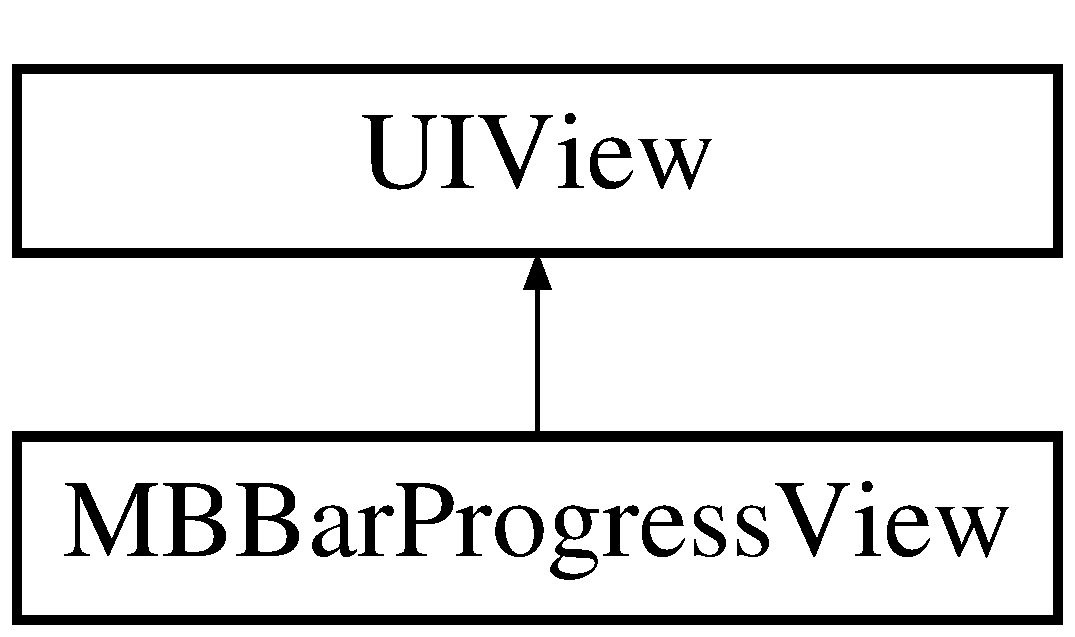
\includegraphics[height=2.000000cm]{interface_m_b_bar_progress_view}
\end{center}
\end{figure}
\subsection*{Properties}
\begin{DoxyCompactItemize}
\item 
float \hyperlink{interface_m_b_bar_progress_view_aa34865ca266850eb7060e91309f3512b}{progress}
\item 
U\+I\+Color $\ast$ \hyperlink{interface_m_b_bar_progress_view_a594029fb5ed62f3de81902c0ea815f2f}{line\+Color}
\item 
U\+I\+Color $\ast$ \hyperlink{interface_m_b_bar_progress_view_a0529e715ce6e40bf0e09864ba0ca1219}{progress\+Remaining\+Color}
\item 
U\+I\+Color $\ast$ \hyperlink{interface_m_b_bar_progress_view_a5b27bb23bd54ae1c7b37a3fedd817e80}{progress\+Color}
\end{DoxyCompactItemize}


\subsection{Detailed Description}
A flat bar progress view. 

Definition at line 475 of file M\+B\+Progress\+H\+U\+D.\+h.



\subsection{Property Documentation}
\hypertarget{interface_m_b_bar_progress_view_a594029fb5ed62f3de81902c0ea815f2f}{\index{M\+B\+Bar\+Progress\+View@{M\+B\+Bar\+Progress\+View}!line\+Color@{line\+Color}}
\index{line\+Color@{line\+Color}!M\+B\+Bar\+Progress\+View@{M\+B\+Bar\+Progress\+View}}
\subsubsection[{line\+Color}]{\setlength{\rightskip}{0pt plus 5cm}-\/ (U\+I\+Color$\ast$) line\+Color\hspace{0.3cm}{\ttfamily [read]}, {\ttfamily [write]}, {\ttfamily [nonatomic]}, {\ttfamily [assign]}}}\label{interface_m_b_bar_progress_view_a594029fb5ed62f3de81902c0ea815f2f}
Bar border line color. Defaults to white \mbox{[}U\+I\+Color white\+Color\mbox{]}. 

Definition at line 486 of file M\+B\+Progress\+H\+U\+D.\+h.

\hypertarget{interface_m_b_bar_progress_view_aa34865ca266850eb7060e91309f3512b}{\index{M\+B\+Bar\+Progress\+View@{M\+B\+Bar\+Progress\+View}!progress@{progress}}
\index{progress@{progress}!M\+B\+Bar\+Progress\+View@{M\+B\+Bar\+Progress\+View}}
\subsubsection[{progress}]{\setlength{\rightskip}{0pt plus 5cm}-\/ (float) progress\hspace{0.3cm}{\ttfamily [read]}, {\ttfamily [write]}, {\ttfamily [nonatomic]}, {\ttfamily [assign]}}}\label{interface_m_b_bar_progress_view_aa34865ca266850eb7060e91309f3512b}
Progress (0.\+0 to 1.\+0) 

Definition at line 480 of file M\+B\+Progress\+H\+U\+D.\+h.

\hypertarget{interface_m_b_bar_progress_view_a5b27bb23bd54ae1c7b37a3fedd817e80}{\index{M\+B\+Bar\+Progress\+View@{M\+B\+Bar\+Progress\+View}!progress\+Color@{progress\+Color}}
\index{progress\+Color@{progress\+Color}!M\+B\+Bar\+Progress\+View@{M\+B\+Bar\+Progress\+View}}
\subsubsection[{progress\+Color}]{\setlength{\rightskip}{0pt plus 5cm}-\/ (U\+I\+Color$\ast$) progress\+Color\hspace{0.3cm}{\ttfamily [read]}, {\ttfamily [write]}, {\ttfamily [nonatomic]}, {\ttfamily [assign]}}}\label{interface_m_b_bar_progress_view_a5b27bb23bd54ae1c7b37a3fedd817e80}
Bar progress color. Defaults to white \mbox{[}U\+I\+Color white\+Color\mbox{]}. 

Definition at line 498 of file M\+B\+Progress\+H\+U\+D.\+h.

\hypertarget{interface_m_b_bar_progress_view_a0529e715ce6e40bf0e09864ba0ca1219}{\index{M\+B\+Bar\+Progress\+View@{M\+B\+Bar\+Progress\+View}!progress\+Remaining\+Color@{progress\+Remaining\+Color}}
\index{progress\+Remaining\+Color@{progress\+Remaining\+Color}!M\+B\+Bar\+Progress\+View@{M\+B\+Bar\+Progress\+View}}
\subsubsection[{progress\+Remaining\+Color}]{\setlength{\rightskip}{0pt plus 5cm}-\/ (U\+I\+Color$\ast$) progress\+Remaining\+Color\hspace{0.3cm}{\ttfamily [read]}, {\ttfamily [write]}, {\ttfamily [nonatomic]}, {\ttfamily [assign]}}}\label{interface_m_b_bar_progress_view_a0529e715ce6e40bf0e09864ba0ca1219}
Bar background color. Defaults to clear \mbox{[}U\+I\+Color clear\+Color\mbox{]}; 

Definition at line 492 of file M\+B\+Progress\+H\+U\+D.\+h.



The documentation for this class was generated from the following file\+:\begin{DoxyCompactItemize}
\item 
Misfit\+Heart\+Rate/\+Utilities/\hyperlink{_m_b_progress_h_u_d_8h}{M\+B\+Progress\+H\+U\+D.\+h}\end{DoxyCompactItemize}

\hypertarget{interface_m_b_progress_h_u_d}{\section{M\+B\+Progress\+H\+U\+D Class Reference}
\label{interface_m_b_progress_h_u_d}\index{M\+B\+Progress\+H\+U\+D@{M\+B\+Progress\+H\+U\+D}}
}


{\ttfamily \#import $<$M\+B\+Progress\+H\+U\+D.\+h$>$}

Inheritance diagram for M\+B\+Progress\+H\+U\+D\+:\begin{figure}[H]
\begin{center}
\leavevmode
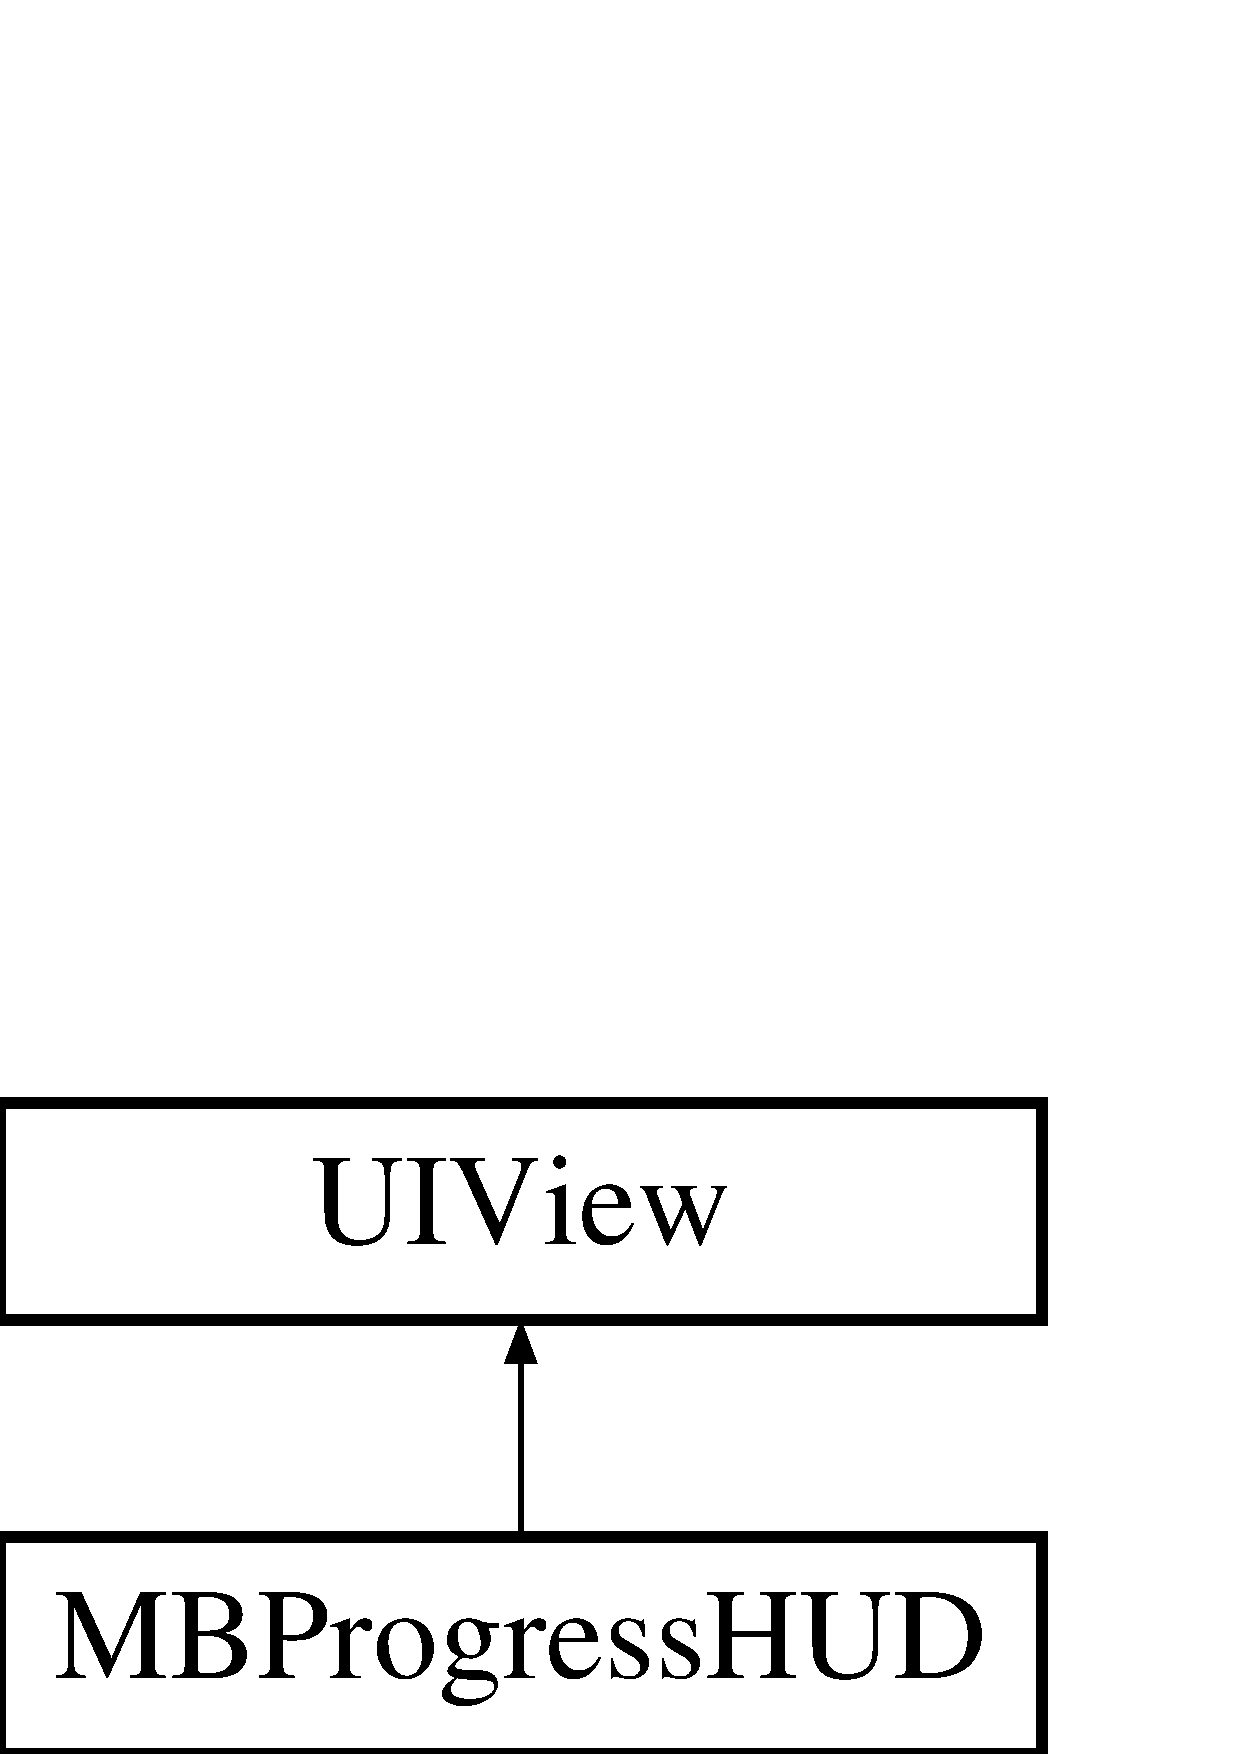
\includegraphics[height=2.000000cm]{interface_m_b_progress_h_u_d}
\end{center}
\end{figure}
\subsection*{Instance Methods}
\begin{DoxyCompactItemize}
\item 
(id) -\/ \hyperlink{interface_m_b_progress_h_u_d_a8f3c01167d59153c85ae7efdca7717fc}{init\+With\+Window\+:}
\item 
(id) -\/ \hyperlink{interface_m_b_progress_h_u_d_ae42ee0d2d0ea58fac1ce8de6b5ea3b60}{init\+With\+View\+:}
\item 
(void) -\/ \hyperlink{interface_m_b_progress_h_u_d_a3ef075a3be624c2f94629d63bfeae25b}{show\+:}
\item 
(void) -\/ \hyperlink{interface_m_b_progress_h_u_d_a500fd79859e56cf98fd2eebfd37b4204}{hide\+:}
\item 
(void) -\/ \hyperlink{interface_m_b_progress_h_u_d_aec6533c21bf8a9f3e552cb133ef6aeed}{hide\+:after\+Delay\+:}
\item 
(void) -\/ \hyperlink{interface_m_b_progress_h_u_d_a23cd23b9c46bd819f14314426ed9dcdb}{show\+While\+Executing\+:on\+Target\+:with\+Object\+:animated\+:}
\end{DoxyCompactItemize}
\subsection*{Class Methods}
\begin{DoxyCompactItemize}
\item 
(\hyperlink{_m_b_progress_h_u_d_8h_a3b2863c8570213ff818b8e2361014d34}{M\+B\+\_\+\+I\+N\+S\+T\+A\+N\+C\+E\+T\+Y\+P\+E}) + \hyperlink{interface_m_b_progress_h_u_d_a85d0c8c9647c47a289e7e7ea5d477c9a}{show\+H\+U\+D\+Added\+To\+:animated\+:}
\item 
(B\+O\+O\+L) + \hyperlink{interface_m_b_progress_h_u_d_ab7a06aebc0d49b4fc963815ad424013f}{hide\+H\+U\+D\+For\+View\+:animated\+:}
\item 
(N\+S\+U\+Integer) + \hyperlink{interface_m_b_progress_h_u_d_a86053d76e84d0fdf033af091df5ea239}{hide\+All\+H\+U\+Ds\+For\+View\+:animated\+:}
\item 
(\hyperlink{_m_b_progress_h_u_d_8h_a3b2863c8570213ff818b8e2361014d34}{M\+B\+\_\+\+I\+N\+S\+T\+A\+N\+C\+E\+T\+Y\+P\+E}) + \hyperlink{interface_m_b_progress_h_u_d_a30afd912f412c6612eee7f1e17241b5b}{H\+U\+D\+For\+View\+:}
\item 
(N\+S\+Array $\ast$) + \hyperlink{interface_m_b_progress_h_u_d_aaa8882a53b5edfd617b4ba112c60811b}{all\+H\+U\+Ds\+For\+View\+:}
\end{DoxyCompactItemize}
\subsection*{Properties}
\begin{DoxyCompactItemize}
\item 
\hyperlink{_m_b_progress_h_u_d_8h_a553b6bab1602fa03257edde8491bb621}{M\+B\+Progress\+H\+U\+D\+Mode} \hyperlink{interface_m_b_progress_h_u_d_ace77eaaf507e86fe56436f7ee7b6fdc9}{mode}
\item 
\hyperlink{_m_b_progress_h_u_d_8h_a892ebf586d23b21a74bc54138ca25990}{M\+B\+Progress\+H\+U\+D\+Animation} \hyperlink{interface_m_b_progress_h_u_d_a71d04bb9e2839df9377ad10d03b2e468}{animation\+Type}
\item 
U\+I\+View $\ast$ \hyperlink{interface_m_b_progress_h_u_d_a78f89e05d797a46bf9b41a5dfd1f5d4a}{custom\+View}
\item 
id$<$ \hyperlink{protocol_m_b_progress_h_u_d_delegate-p}{M\+B\+Progress\+H\+U\+D\+Delegate} $>$ \hyperlink{interface_m_b_progress_h_u_d_ad6fee32939fa55fc1a341aba117aa28f}{delegate}
\item 
N\+S\+String $\ast$ \hyperlink{interface_m_b_progress_h_u_d_a531706887f08881c7f13b4309521b299}{label\+Text}
\item 
N\+S\+String $\ast$ \hyperlink{interface_m_b_progress_h_u_d_a8b7cbf551fc551c64159b7a3f648c6ac}{details\+Label\+Text}
\item 
float \hyperlink{interface_m_b_progress_h_u_d_a24ab5e37917e3489d6add081324a49ff}{opacity}
\item 
U\+I\+Color $\ast$ \hyperlink{interface_m_b_progress_h_u_d_a1f4ab0f3ddc52af9353a4cf225ad1361}{color}
\item 
float \hyperlink{interface_m_b_progress_h_u_d_a4e6ee114c04b90ced1a253a6d33ba785}{x\+Offset}
\item 
float \hyperlink{interface_m_b_progress_h_u_d_ad526ffcabab5131697eb0850c50ab1f4}{y\+Offset}
\item 
float \hyperlink{interface_m_b_progress_h_u_d_a4126e72234f8afcb87905a9ed65c022c}{margin}
\item 
float \hyperlink{interface_m_b_progress_h_u_d_a8a3573dbf4dcdeeb187a08d0070e811c}{corner\+Radius}
\item 
B\+O\+O\+L \hyperlink{interface_m_b_progress_h_u_d_ab781ccd4428c8eff6907d2cdc90fc3ee}{dim\+Background}
\item 
float \hyperlink{interface_m_b_progress_h_u_d_a6f837c351a405d0bb6ec05856d7776dd}{grace\+Time}
\item 
float \hyperlink{interface_m_b_progress_h_u_d_a9946e4b0b16d75f070ff0cbcc50226ef}{min\+Show\+Time}
\item 
B\+O\+O\+L \hyperlink{interface_m_b_progress_h_u_d_a6077ea42c37c18b3058ed63ac10ede8f}{task\+In\+Progress}
\item 
B\+O\+O\+L \hyperlink{interface_m_b_progress_h_u_d_a36639aa18a70f2734942695c32ec5e91}{remove\+From\+Super\+View\+On\+Hide}
\item 
U\+I\+Font $\ast$ \hyperlink{interface_m_b_progress_h_u_d_ae61e736a34f341f4190b065f19010af8}{label\+Font}
\item 
U\+I\+Color $\ast$ \hyperlink{interface_m_b_progress_h_u_d_a04eba696a66f65d28b485bb5f0a940cd}{label\+Color}
\item 
U\+I\+Font $\ast$ \hyperlink{interface_m_b_progress_h_u_d_af070a363d323d8eb0285e38d398b51c2}{details\+Label\+Font}
\item 
U\+I\+Color $\ast$ \hyperlink{interface_m_b_progress_h_u_d_ace929217bd7673159f063d5b8e80b080}{details\+Label\+Color}
\item 
float \hyperlink{interface_m_b_progress_h_u_d_a4c8328617d11efd1f5452032246ca97f}{progress}
\item 
C\+G\+Size \hyperlink{interface_m_b_progress_h_u_d_a69c6b2cad533d6fe7d90df02bf7f8b0c}{min\+Size}
\item 
B\+O\+O\+L \hyperlink{interface_m_b_progress_h_u_d_a4bf7271b213e304259aa7d97f7cb1849}{square}
\end{DoxyCompactItemize}


\subsection{Detailed Description}
Displays a simple H\+U\+D window containing a progress indicator and two optional labels for short messages.

This is a simple drop-\/in class for displaying a progress H\+U\+D view similar to Apple's private U\+I\+Progress\+H\+U\+D class. The \hyperlink{interface_m_b_progress_h_u_d}{M\+B\+Progress\+H\+U\+D} window spans over the entire space given to it by the init\+With\+Frame constructor and catches all user input on this region, thereby preventing the user operations on components below the view. The H\+U\+D itself is drawn centered as a rounded semi-\/transparent view which resizes depending on the user specified content.

This view supports four modes of operation\+:
\begin{DoxyItemize}
\item M\+B\+Progress\+H\+U\+D\+Mode\+Indeterminate -\/ shows a U\+I\+Activity\+Indicator\+View
\item M\+B\+Progress\+H\+U\+D\+Mode\+Determinate -\/ shows a custom round progress indicator
\item M\+B\+Progress\+H\+U\+D\+Mode\+Annular\+Determinate -\/ shows a custom annular progress indicator
\item M\+B\+Progress\+H\+U\+D\+Mode\+Custom\+View -\/ shows an arbitrary, user specified view (\begin{DoxySeeAlso}{See also}
\hyperlink{interface_m_b_progress_h_u_d_a78f89e05d797a46bf9b41a5dfd1f5d4a}{custom\+View})
\end{DoxySeeAlso}
All three modes can have optional labels assigned\+:
\item If the label\+Text property is set and non-\/empty then a label containing the provided content is placed below the indicator view.
\item If also the details\+Label\+Text property is set then another label is placed below the first label. 
\end{DoxyItemize}

Definition at line 111 of file M\+B\+Progress\+H\+U\+D.\+h.



\subsection{Method Documentation}
\hypertarget{interface_m_b_progress_h_u_d_aaa8882a53b5edfd617b4ba112c60811b}{\index{M\+B\+Progress\+H\+U\+D@{M\+B\+Progress\+H\+U\+D}!all\+H\+U\+Ds\+For\+View\+:@{all\+H\+U\+Ds\+For\+View\+:}}
\index{all\+H\+U\+Ds\+For\+View\+:@{all\+H\+U\+Ds\+For\+View\+:}!M\+B\+Progress\+H\+U\+D@{M\+B\+Progress\+H\+U\+D}}
\subsubsection[{all\+H\+U\+Ds\+For\+View\+:}]{\setlength{\rightskip}{0pt plus 5cm}+ (N\+S\+Array $\ast$) all\+H\+U\+Ds\+For\+View\+: 
\begin{DoxyParamCaption}
\item[{(U\+I\+View $\ast$)}]{view}
\end{DoxyParamCaption}
}}\label{interface_m_b_progress_h_u_d_aaa8882a53b5edfd617b4ba112c60811b}
Finds all H\+U\+D subviews and returns them.


\begin{DoxyParams}{Parameters}
{\em view} & The view that is going to be searched. \\
\hline
\end{DoxyParams}
\begin{DoxyReturn}{Returns}
All found H\+U\+D views (array of \hyperlink{interface_m_b_progress_h_u_d}{M\+B\+Progress\+H\+U\+D} objects). 
\end{DoxyReturn}


Definition at line 162 of file M\+B\+Progress\+H\+U\+D.\+m.

\hypertarget{interface_m_b_progress_h_u_d_a500fd79859e56cf98fd2eebfd37b4204}{\index{M\+B\+Progress\+H\+U\+D@{M\+B\+Progress\+H\+U\+D}!hide\+:@{hide\+:}}
\index{hide\+:@{hide\+:}!M\+B\+Progress\+H\+U\+D@{M\+B\+Progress\+H\+U\+D}}
\subsubsection[{hide\+:}]{\setlength{\rightskip}{0pt plus 5cm}-\/ (void) hide\+: 
\begin{DoxyParamCaption}
\item[{(B\+O\+O\+L)}]{animated}
\end{DoxyParamCaption}
}}\label{interface_m_b_progress_h_u_d_a500fd79859e56cf98fd2eebfd37b4204}
Hide the H\+U\+D. This still calls the hud\+Was\+Hidden\+: delegate. This is the counterpart of the show\+: method. Use it to hide the H\+U\+D when your task completes.


\begin{DoxyParams}{Parameters}
{\em animated} & If set to Y\+E\+S the H\+U\+D will disappear using the current animation\+Type. If set to N\+O the H\+U\+D will not use animations while disappearing.\\
\hline
\end{DoxyParams}
\begin{DoxySeeAlso}{See also}
\hyperlink{interface_m_b_progress_h_u_d_a71d04bb9e2839df9377ad10d03b2e468}{animation\+Type} 
\end{DoxySeeAlso}


Definition at line 269 of file M\+B\+Progress\+H\+U\+D.\+m.

\hypertarget{interface_m_b_progress_h_u_d_aec6533c21bf8a9f3e552cb133ef6aeed}{\index{M\+B\+Progress\+H\+U\+D@{M\+B\+Progress\+H\+U\+D}!hide\+:after\+Delay\+:@{hide\+:after\+Delay\+:}}
\index{hide\+:after\+Delay\+:@{hide\+:after\+Delay\+:}!M\+B\+Progress\+H\+U\+D@{M\+B\+Progress\+H\+U\+D}}
\subsubsection[{hide\+:after\+Delay\+:}]{\setlength{\rightskip}{0pt plus 5cm}-\/ (void) {\bf hide\+:} 
\begin{DoxyParamCaption}
\item[{(B\+O\+O\+L)}]{animated}
\item[{afterDelay:(N\+S\+Time\+Interval)}]{delay}
\end{DoxyParamCaption}
}}\label{interface_m_b_progress_h_u_d_aec6533c21bf8a9f3e552cb133ef6aeed}
Hide the H\+U\+D after a delay. This still calls the hud\+Was\+Hidden\+: delegate. This is the counterpart of the show\+: method. Use it to hide the H\+U\+D when your task completes.


\begin{DoxyParams}{Parameters}
{\em animated} & If set to Y\+E\+S the H\+U\+D will disappear using the current animation\+Type. If set to N\+O the H\+U\+D will not use animations while disappearing. \\
\hline
{\em delay} & Delay in seconds until the H\+U\+D is hidden.\\
\hline
\end{DoxyParams}
\begin{DoxySeeAlso}{See also}
\hyperlink{interface_m_b_progress_h_u_d_a71d04bb9e2839df9377ad10d03b2e468}{animation\+Type} 
\end{DoxySeeAlso}


Definition at line 285 of file M\+B\+Progress\+H\+U\+D.\+m.

\hypertarget{interface_m_b_progress_h_u_d_a86053d76e84d0fdf033af091df5ea239}{\index{M\+B\+Progress\+H\+U\+D@{M\+B\+Progress\+H\+U\+D}!hide\+All\+H\+U\+Ds\+For\+View\+:animated\+:@{hide\+All\+H\+U\+Ds\+For\+View\+:animated\+:}}
\index{hide\+All\+H\+U\+Ds\+For\+View\+:animated\+:@{hide\+All\+H\+U\+Ds\+For\+View\+:animated\+:}!M\+B\+Progress\+H\+U\+D@{M\+B\+Progress\+H\+U\+D}}
\subsubsection[{hide\+All\+H\+U\+Ds\+For\+View\+:animated\+:}]{\setlength{\rightskip}{0pt plus 5cm}+ (N\+S\+U\+Integer) hide\+All\+H\+U\+Ds\+For\+View\+: 
\begin{DoxyParamCaption}
\item[{(U\+I\+View $\ast$)}]{view}
\item[{animated:(B\+O\+O\+L)}]{animated}
\end{DoxyParamCaption}
}}\label{interface_m_b_progress_h_u_d_a86053d76e84d0fdf033af091df5ea239}
Finds all the H\+U\+D subviews and hides them.


\begin{DoxyParams}{Parameters}
{\em view} & The view that is going to be searched for H\+U\+D subviews. \\
\hline
{\em animated} & If set to Y\+E\+S the H\+U\+Ds will disappear using the current animation\+Type. If set to N\+O the H\+U\+Ds will not use animations while disappearing. \\
\hline
\end{DoxyParams}
\begin{DoxyReturn}{Returns}
the number of H\+U\+Ds found and removed.
\end{DoxyReturn}
\begin{DoxySeeAlso}{See also}
\hyperlink{interface_m_b_progress_h_u_d_ab7a06aebc0d49b4fc963815ad424013f}{+ hide\+H\+U\+D\+For\+View\+:animated\+:} 

\hyperlink{interface_m_b_progress_h_u_d_a71d04bb9e2839df9377ad10d03b2e468}{animation\+Type} 
\end{DoxySeeAlso}


Definition at line 143 of file M\+B\+Progress\+H\+U\+D.\+m.

\hypertarget{interface_m_b_progress_h_u_d_ab7a06aebc0d49b4fc963815ad424013f}{\index{M\+B\+Progress\+H\+U\+D@{M\+B\+Progress\+H\+U\+D}!hide\+H\+U\+D\+For\+View\+:animated\+:@{hide\+H\+U\+D\+For\+View\+:animated\+:}}
\index{hide\+H\+U\+D\+For\+View\+:animated\+:@{hide\+H\+U\+D\+For\+View\+:animated\+:}!M\+B\+Progress\+H\+U\+D@{M\+B\+Progress\+H\+U\+D}}
\subsubsection[{hide\+H\+U\+D\+For\+View\+:animated\+:}]{\setlength{\rightskip}{0pt plus 5cm}+ (B\+O\+O\+L) hide\+H\+U\+D\+For\+View\+: 
\begin{DoxyParamCaption}
\item[{(U\+I\+View $\ast$)}]{view}
\item[{animated:(B\+O\+O\+L)}]{animated}
\end{DoxyParamCaption}
}}\label{interface_m_b_progress_h_u_d_ab7a06aebc0d49b4fc963815ad424013f}
Finds the top-\/most H\+U\+D subview and hides it. The counterpart to this method is show\+H\+U\+D\+Added\+To\+:animated\+:.


\begin{DoxyParams}{Parameters}
{\em view} & The view that is going to be searched for a H\+U\+D subview. \\
\hline
{\em animated} & If set to Y\+E\+S the H\+U\+D will disappear using the current animation\+Type. If set to N\+O the H\+U\+D will not use animations while disappearing. \\
\hline
\end{DoxyParams}
\begin{DoxyReturn}{Returns}
Y\+E\+S if a H\+U\+D was found and removed, N\+O otherwise.
\end{DoxyReturn}
\begin{DoxySeeAlso}{See also}
\hyperlink{interface_m_b_progress_h_u_d_a85d0c8c9647c47a289e7e7ea5d477c9a}{+ show\+H\+U\+D\+Added\+To\+:animated\+:} 

\hyperlink{interface_m_b_progress_h_u_d_a71d04bb9e2839df9377ad10d03b2e468}{animation\+Type} 
\end{DoxySeeAlso}


Definition at line 133 of file M\+B\+Progress\+H\+U\+D.\+m.

\hypertarget{interface_m_b_progress_h_u_d_a30afd912f412c6612eee7f1e17241b5b}{\index{M\+B\+Progress\+H\+U\+D@{M\+B\+Progress\+H\+U\+D}!H\+U\+D\+For\+View\+:@{H\+U\+D\+For\+View\+:}}
\index{H\+U\+D\+For\+View\+:@{H\+U\+D\+For\+View\+:}!M\+B\+Progress\+H\+U\+D@{M\+B\+Progress\+H\+U\+D}}
\subsubsection[{H\+U\+D\+For\+View\+:}]{\setlength{\rightskip}{0pt plus 5cm}+ ({\bf M\+B\+\_\+\+I\+N\+S\+T\+A\+N\+C\+E\+T\+Y\+P\+E}) H\+U\+D\+For\+View\+: 
\begin{DoxyParamCaption}
\item[{(U\+I\+View $\ast$)}]{view}
\end{DoxyParamCaption}
}}\label{interface_m_b_progress_h_u_d_a30afd912f412c6612eee7f1e17241b5b}
Finds the top-\/most H\+U\+D subview and returns it.


\begin{DoxyParams}{Parameters}
{\em view} & The view that is going to be searched. \\
\hline
\end{DoxyParams}
\begin{DoxyReturn}{Returns}
A reference to the last H\+U\+D subview discovered. 
\end{DoxyReturn}


Definition at line 152 of file M\+B\+Progress\+H\+U\+D.\+m.

\hypertarget{interface_m_b_progress_h_u_d_ae42ee0d2d0ea58fac1ce8de6b5ea3b60}{\index{M\+B\+Progress\+H\+U\+D@{M\+B\+Progress\+H\+U\+D}!init\+With\+View\+:@{init\+With\+View\+:}}
\index{init\+With\+View\+:@{init\+With\+View\+:}!M\+B\+Progress\+H\+U\+D@{M\+B\+Progress\+H\+U\+D}}
\subsubsection[{init\+With\+View\+:}]{\setlength{\rightskip}{0pt plus 5cm}-\/ (id) init\+With\+View\+: 
\begin{DoxyParamCaption}
\item[{(U\+I\+View $\ast$)}]{view}
\end{DoxyParamCaption}
}}\label{interface_m_b_progress_h_u_d_ae42ee0d2d0ea58fac1ce8de6b5ea3b60}
A convenience constructor that initializes the H\+U\+D with the view's bounds. Calls the designated constructor with view.\+bounds as the parameter


\begin{DoxyParams}{Parameters}
{\em view} & The view instance that will provide the bounds for the H\+U\+D. Should be the same instance as the H\+U\+D's superview (i.\+e., the view that the H\+U\+D will be added to). \\
\hline
\end{DoxyParams}


Definition at line 219 of file M\+B\+Progress\+H\+U\+D.\+m.

\hypertarget{interface_m_b_progress_h_u_d_a8f3c01167d59153c85ae7efdca7717fc}{\index{M\+B\+Progress\+H\+U\+D@{M\+B\+Progress\+H\+U\+D}!init\+With\+Window\+:@{init\+With\+Window\+:}}
\index{init\+With\+Window\+:@{init\+With\+Window\+:}!M\+B\+Progress\+H\+U\+D@{M\+B\+Progress\+H\+U\+D}}
\subsubsection[{init\+With\+Window\+:}]{\setlength{\rightskip}{0pt plus 5cm}-\/ (id) init\+With\+Window\+: 
\begin{DoxyParamCaption}
\item[{(U\+I\+Window $\ast$)}]{window}
\end{DoxyParamCaption}
}}\label{interface_m_b_progress_h_u_d_a8f3c01167d59153c85ae7efdca7717fc}
A convenience constructor that initializes the H\+U\+D with the window's bounds. Calls the designated constructor with window.\+bounds as the parameter.


\begin{DoxyParams}{Parameters}
{\em window} & The window instance that will provide the bounds for the H\+U\+D. Should be the same instance as the H\+U\+D's superview (i.\+e., the window that the H\+U\+D will be added to). \\
\hline
\end{DoxyParams}


Definition at line 224 of file M\+B\+Progress\+H\+U\+D.\+m.

\hypertarget{interface_m_b_progress_h_u_d_a3ef075a3be624c2f94629d63bfeae25b}{\index{M\+B\+Progress\+H\+U\+D@{M\+B\+Progress\+H\+U\+D}!show\+:@{show\+:}}
\index{show\+:@{show\+:}!M\+B\+Progress\+H\+U\+D@{M\+B\+Progress\+H\+U\+D}}
\subsubsection[{show\+:}]{\setlength{\rightskip}{0pt plus 5cm}-\/ (void) show\+: 
\begin{DoxyParamCaption}
\item[{(B\+O\+O\+L)}]{animated}
\end{DoxyParamCaption}
}}\label{interface_m_b_progress_h_u_d_a3ef075a3be624c2f94629d63bfeae25b}
Display the H\+U\+D. You need to make sure that the main thread completes its run loop soon after this method call so the user interface can be updated. Call this method when your task is already set-\/up to be executed in a new thread (e.\+g., when using something like N\+S\+Operation or calling an asynchronous call like N\+S\+U\+R\+L\+Request).


\begin{DoxyParams}{Parameters}
{\em animated} & If set to Y\+E\+S the H\+U\+D will appear using the current animation\+Type. If set to N\+O the H\+U\+D will not use animations while appearing.\\
\hline
\end{DoxyParams}
\begin{DoxySeeAlso}{See also}
\hyperlink{interface_m_b_progress_h_u_d_a71d04bb9e2839df9377ad10d03b2e468}{animation\+Type} 
\end{DoxySeeAlso}


Definition at line 255 of file M\+B\+Progress\+H\+U\+D.\+m.

\hypertarget{interface_m_b_progress_h_u_d_a85d0c8c9647c47a289e7e7ea5d477c9a}{\index{M\+B\+Progress\+H\+U\+D@{M\+B\+Progress\+H\+U\+D}!show\+H\+U\+D\+Added\+To\+:animated\+:@{show\+H\+U\+D\+Added\+To\+:animated\+:}}
\index{show\+H\+U\+D\+Added\+To\+:animated\+:@{show\+H\+U\+D\+Added\+To\+:animated\+:}!M\+B\+Progress\+H\+U\+D@{M\+B\+Progress\+H\+U\+D}}
\subsubsection[{show\+H\+U\+D\+Added\+To\+:animated\+:}]{\setlength{\rightskip}{0pt plus 5cm}+ ({\bf M\+B\+\_\+\+I\+N\+S\+T\+A\+N\+C\+E\+T\+Y\+P\+E}) show\+H\+U\+D\+Added\+To\+: 
\begin{DoxyParamCaption}
\item[{(U\+I\+View $\ast$)}]{view}
\item[{animated:(B\+O\+O\+L)}]{animated}
\end{DoxyParamCaption}
}}\label{interface_m_b_progress_h_u_d_a85d0c8c9647c47a289e7e7ea5d477c9a}
Creates a new H\+U\+D, adds it to provided view and shows it. The counterpart to this method is hide\+H\+U\+D\+For\+View\+:animated\+:.


\begin{DoxyParams}{Parameters}
{\em view} & The view that the H\+U\+D will be added to \\
\hline
{\em animated} & If set to Y\+E\+S the H\+U\+D will appear using the current animation\+Type. If set to N\+O the H\+U\+D will not use animations while appearing. \\
\hline
\end{DoxyParams}
\begin{DoxyReturn}{Returns}
A reference to the created H\+U\+D.
\end{DoxyReturn}
\begin{DoxySeeAlso}{See also}
\hyperlink{interface_m_b_progress_h_u_d_ab7a06aebc0d49b4fc963815ad424013f}{+ hide\+H\+U\+D\+For\+View\+:animated\+:} 

\hyperlink{interface_m_b_progress_h_u_d_a71d04bb9e2839df9377ad10d03b2e468}{animation\+Type} 
\end{DoxySeeAlso}


Definition at line 126 of file M\+B\+Progress\+H\+U\+D.\+m.

\hypertarget{interface_m_b_progress_h_u_d_a23cd23b9c46bd819f14314426ed9dcdb}{\index{M\+B\+Progress\+H\+U\+D@{M\+B\+Progress\+H\+U\+D}!show\+While\+Executing\+:on\+Target\+:with\+Object\+:animated\+:@{show\+While\+Executing\+:on\+Target\+:with\+Object\+:animated\+:}}
\index{show\+While\+Executing\+:on\+Target\+:with\+Object\+:animated\+:@{show\+While\+Executing\+:on\+Target\+:with\+Object\+:animated\+:}!M\+B\+Progress\+H\+U\+D@{M\+B\+Progress\+H\+U\+D}}
\subsubsection[{show\+While\+Executing\+:on\+Target\+:with\+Object\+:animated\+:}]{\setlength{\rightskip}{0pt plus 5cm}-\/ (void) show\+While\+Executing\+: 
\begin{DoxyParamCaption}
\item[{(S\+E\+L)}]{method}
\item[{onTarget:(id)}]{target}
\item[{withObject:(id)}]{object}
\item[{animated:(B\+O\+O\+L)}]{animated}
\end{DoxyParamCaption}
}}\label{interface_m_b_progress_h_u_d_a23cd23b9c46bd819f14314426ed9dcdb}
Shows the H\+U\+D while a background task is executing in a new thread, then hides the H\+U\+D.

This method also takes care of autorelease pools so your method does not have to be concerned with setting up a pool.


\begin{DoxyParams}{Parameters}
{\em method} & The method to be executed while the H\+U\+D is shown. This method will be executed in a new thread. \\
\hline
{\em target} & The object that the target method belongs to. \\
\hline
{\em object} & An optional object to be passed to the method. \\
\hline
{\em animated} & If set to Y\+E\+S the H\+U\+D will (dis)appear using the current animation\+Type. If set to N\+O the H\+U\+D will not use animations while (dis)appearing. \\
\hline
\end{DoxyParams}


Definition at line 389 of file M\+B\+Progress\+H\+U\+D.\+m.



\subsection{Property Documentation}
\hypertarget{interface_m_b_progress_h_u_d_a71d04bb9e2839df9377ad10d03b2e468}{\index{M\+B\+Progress\+H\+U\+D@{M\+B\+Progress\+H\+U\+D}!animation\+Type@{animation\+Type}}
\index{animation\+Type@{animation\+Type}!M\+B\+Progress\+H\+U\+D@{M\+B\+Progress\+H\+U\+D}}
\subsubsection[{animation\+Type}]{\setlength{\rightskip}{0pt plus 5cm}-\/ ({\bf M\+B\+Progress\+H\+U\+D\+Animation}) animation\+Type\hspace{0.3cm}{\ttfamily [read]}, {\ttfamily [write]}, {\ttfamily [atomic]}, {\ttfamily [assign]}}}\label{interface_m_b_progress_h_u_d_a71d04bb9e2839df9377ad10d03b2e468}
The animation type that should be used when the H\+U\+D is shown and hidden.

\begin{DoxySeeAlso}{See also}
\hyperlink{_m_b_progress_h_u_d_8h_a892ebf586d23b21a74bc54138ca25990}{M\+B\+Progress\+H\+U\+D\+Animation} 
\end{DoxySeeAlso}


Definition at line 291 of file M\+B\+Progress\+H\+U\+D.\+h.

\hypertarget{interface_m_b_progress_h_u_d_a1f4ab0f3ddc52af9353a4cf225ad1361}{\index{M\+B\+Progress\+H\+U\+D@{M\+B\+Progress\+H\+U\+D}!color@{color}}
\index{color@{color}!M\+B\+Progress\+H\+U\+D@{M\+B\+Progress\+H\+U\+D}}
\subsubsection[{color}]{\setlength{\rightskip}{0pt plus 5cm}-\/ (U\+I\+Color$\ast$) color\hspace{0.3cm}{\ttfamily [read]}, {\ttfamily [write]}, {\ttfamily [atomic]}, {\ttfamily [assign]}}}\label{interface_m_b_progress_h_u_d_a1f4ab0f3ddc52af9353a4cf225ad1361}
The color of the H\+U\+D window. Defaults to black. If this property is set, color is set using this U\+I\+Color and the opacity property is not used. using retain because performing copy on U\+I\+Color base colors (like \mbox{[}U\+I\+Color green\+Color\mbox{]}) cause problems with the copy\+Zone. 

Definition at line 329 of file M\+B\+Progress\+H\+U\+D.\+h.

\hypertarget{interface_m_b_progress_h_u_d_a8a3573dbf4dcdeeb187a08d0070e811c}{\index{M\+B\+Progress\+H\+U\+D@{M\+B\+Progress\+H\+U\+D}!corner\+Radius@{corner\+Radius}}
\index{corner\+Radius@{corner\+Radius}!M\+B\+Progress\+H\+U\+D@{M\+B\+Progress\+H\+U\+D}}
\subsubsection[{corner\+Radius}]{\setlength{\rightskip}{0pt plus 5cm}-\/ (float) corner\+Radius\hspace{0.3cm}{\ttfamily [read]}, {\ttfamily [write]}, {\ttfamily [atomic]}, {\ttfamily [assign]}}}\label{interface_m_b_progress_h_u_d_a8a3573dbf4dcdeeb187a08d0070e811c}
The corner radius for th H\+U\+D Defaults to 10.\+0 

Definition at line 351 of file M\+B\+Progress\+H\+U\+D.\+h.

\hypertarget{interface_m_b_progress_h_u_d_a78f89e05d797a46bf9b41a5dfd1f5d4a}{\index{M\+B\+Progress\+H\+U\+D@{M\+B\+Progress\+H\+U\+D}!custom\+View@{custom\+View}}
\index{custom\+View@{custom\+View}!M\+B\+Progress\+H\+U\+D@{M\+B\+Progress\+H\+U\+D}}
\subsubsection[{custom\+View}]{\setlength{\rightskip}{0pt plus 5cm}-\/ (U\+I\+View$\ast$) custom\+View\hspace{0.3cm}{\ttfamily [read]}, {\ttfamily [write]}, {\ttfamily [atomic]}, {\ttfamily [assign]}}}\label{interface_m_b_progress_h_u_d_a78f89e05d797a46bf9b41a5dfd1f5d4a}
The U\+I\+View (e.\+g., a U\+I\+Image\+View) to be shown when the H\+U\+D is in M\+B\+Progress\+H\+U\+D\+Mode\+Custom\+View. For best results use a 37 by 37 pixel view (so the bounds match the built in indicator bounds). 

Definition at line 297 of file M\+B\+Progress\+H\+U\+D.\+h.

\hypertarget{interface_m_b_progress_h_u_d_ad6fee32939fa55fc1a341aba117aa28f}{\index{M\+B\+Progress\+H\+U\+D@{M\+B\+Progress\+H\+U\+D}!delegate@{delegate}}
\index{delegate@{delegate}!M\+B\+Progress\+H\+U\+D@{M\+B\+Progress\+H\+U\+D}}
\subsubsection[{delegate}]{\setlength{\rightskip}{0pt plus 5cm}-\/ (id$<${\bf M\+B\+Progress\+H\+U\+D\+Delegate}$>$) delegate\hspace{0.3cm}{\ttfamily [read]}, {\ttfamily [write]}, {\ttfamily [atomic]}, {\ttfamily [assign]}}}\label{interface_m_b_progress_h_u_d_ad6fee32939fa55fc1a341aba117aa28f}
The H\+U\+D delegate object.

\begin{DoxySeeAlso}{See also}
\hyperlink{protocol_m_b_progress_h_u_d_delegate-p}{M\+B\+Progress\+H\+U\+D\+Delegate} 
\end{DoxySeeAlso}


Definition at line 304 of file M\+B\+Progress\+H\+U\+D.\+h.

\hypertarget{interface_m_b_progress_h_u_d_ace929217bd7673159f063d5b8e80b080}{\index{M\+B\+Progress\+H\+U\+D@{M\+B\+Progress\+H\+U\+D}!details\+Label\+Color@{details\+Label\+Color}}
\index{details\+Label\+Color@{details\+Label\+Color}!M\+B\+Progress\+H\+U\+D@{M\+B\+Progress\+H\+U\+D}}
\subsubsection[{details\+Label\+Color}]{\setlength{\rightskip}{0pt plus 5cm}-\/ (U\+I\+Color$\ast$) details\+Label\+Color\hspace{0.3cm}{\ttfamily [read]}, {\ttfamily [write]}, {\ttfamily [atomic]}, {\ttfamily [assign]}}}\label{interface_m_b_progress_h_u_d_ace929217bd7673159f063d5b8e80b080}
Color to be used for the details label. Set this property if the default is not adequate. 

Definition at line 410 of file M\+B\+Progress\+H\+U\+D.\+h.

\hypertarget{interface_m_b_progress_h_u_d_af070a363d323d8eb0285e38d398b51c2}{\index{M\+B\+Progress\+H\+U\+D@{M\+B\+Progress\+H\+U\+D}!details\+Label\+Font@{details\+Label\+Font}}
\index{details\+Label\+Font@{details\+Label\+Font}!M\+B\+Progress\+H\+U\+D@{M\+B\+Progress\+H\+U\+D}}
\subsubsection[{details\+Label\+Font}]{\setlength{\rightskip}{0pt plus 5cm}-\/ (U\+I\+Font$\ast$) details\+Label\+Font\hspace{0.3cm}{\ttfamily [read]}, {\ttfamily [write]}, {\ttfamily [atomic]}, {\ttfamily [assign]}}}\label{interface_m_b_progress_h_u_d_af070a363d323d8eb0285e38d398b51c2}
Font to be used for the details label. Set this property if the default is not adequate. 

Definition at line 405 of file M\+B\+Progress\+H\+U\+D.\+h.

\hypertarget{interface_m_b_progress_h_u_d_a8b7cbf551fc551c64159b7a3f648c6ac}{\index{M\+B\+Progress\+H\+U\+D@{M\+B\+Progress\+H\+U\+D}!details\+Label\+Text@{details\+Label\+Text}}
\index{details\+Label\+Text@{details\+Label\+Text}!M\+B\+Progress\+H\+U\+D@{M\+B\+Progress\+H\+U\+D}}
\subsubsection[{details\+Label\+Text}]{\setlength{\rightskip}{0pt plus 5cm}-\/ (N\+S\+String$\ast$) details\+Label\+Text\hspace{0.3cm}{\ttfamily [read]}, {\ttfamily [write]}, {\ttfamily [atomic]}, {\ttfamily [copy]}}}\label{interface_m_b_progress_h_u_d_a8b7cbf551fc551c64159b7a3f648c6ac}
An optional details message displayed below the label\+Text message. This message is displayed only if the label\+Text property is also set and is different from an empty string (""). The details text can span multiple lines. 

Definition at line 317 of file M\+B\+Progress\+H\+U\+D.\+h.

\hypertarget{interface_m_b_progress_h_u_d_ab781ccd4428c8eff6907d2cdc90fc3ee}{\index{M\+B\+Progress\+H\+U\+D@{M\+B\+Progress\+H\+U\+D}!dim\+Background@{dim\+Background}}
\index{dim\+Background@{dim\+Background}!M\+B\+Progress\+H\+U\+D@{M\+B\+Progress\+H\+U\+D}}
\subsubsection[{dim\+Background}]{\setlength{\rightskip}{0pt plus 5cm}-\/ (B\+O\+O\+L) dim\+Background\hspace{0.3cm}{\ttfamily [read]}, {\ttfamily [write]}, {\ttfamily [atomic]}, {\ttfamily [assign]}}}\label{interface_m_b_progress_h_u_d_ab781ccd4428c8eff6907d2cdc90fc3ee}
Cover the H\+U\+D background view with a radial gradient. 

Definition at line 356 of file M\+B\+Progress\+H\+U\+D.\+h.

\hypertarget{interface_m_b_progress_h_u_d_a6f837c351a405d0bb6ec05856d7776dd}{\index{M\+B\+Progress\+H\+U\+D@{M\+B\+Progress\+H\+U\+D}!grace\+Time@{grace\+Time}}
\index{grace\+Time@{grace\+Time}!M\+B\+Progress\+H\+U\+D@{M\+B\+Progress\+H\+U\+D}}
\subsubsection[{grace\+Time}]{\setlength{\rightskip}{0pt plus 5cm}-\/ (float) grace\+Time\hspace{0.3cm}{\ttfamily [read]}, {\ttfamily [write]}, {\ttfamily [atomic]}, {\ttfamily [assign]}}}\label{interface_m_b_progress_h_u_d_a6f837c351a405d0bb6ec05856d7776dd}


Definition at line 367 of file M\+B\+Progress\+H\+U\+D.\+h.

\hypertarget{interface_m_b_progress_h_u_d_a04eba696a66f65d28b485bb5f0a940cd}{\index{M\+B\+Progress\+H\+U\+D@{M\+B\+Progress\+H\+U\+D}!label\+Color@{label\+Color}}
\index{label\+Color@{label\+Color}!M\+B\+Progress\+H\+U\+D@{M\+B\+Progress\+H\+U\+D}}
\subsubsection[{label\+Color}]{\setlength{\rightskip}{0pt plus 5cm}-\/ (U\+I\+Color$\ast$) label\+Color\hspace{0.3cm}{\ttfamily [read]}, {\ttfamily [write]}, {\ttfamily [atomic]}, {\ttfamily [assign]}}}\label{interface_m_b_progress_h_u_d_a04eba696a66f65d28b485bb5f0a940cd}
Color to be used for the main label. Set this property if the default is not adequate. 

Definition at line 400 of file M\+B\+Progress\+H\+U\+D.\+h.

\hypertarget{interface_m_b_progress_h_u_d_ae61e736a34f341f4190b065f19010af8}{\index{M\+B\+Progress\+H\+U\+D@{M\+B\+Progress\+H\+U\+D}!label\+Font@{label\+Font}}
\index{label\+Font@{label\+Font}!M\+B\+Progress\+H\+U\+D@{M\+B\+Progress\+H\+U\+D}}
\subsubsection[{label\+Font}]{\setlength{\rightskip}{0pt plus 5cm}-\/ (U\+I\+Font$\ast$) label\+Font\hspace{0.3cm}{\ttfamily [read]}, {\ttfamily [write]}, {\ttfamily [atomic]}, {\ttfamily [assign]}}}\label{interface_m_b_progress_h_u_d_ae61e736a34f341f4190b065f19010af8}
Font to be used for the main label. Set this property if the default is not adequate. 

Definition at line 395 of file M\+B\+Progress\+H\+U\+D.\+h.

\hypertarget{interface_m_b_progress_h_u_d_a531706887f08881c7f13b4309521b299}{\index{M\+B\+Progress\+H\+U\+D@{M\+B\+Progress\+H\+U\+D}!label\+Text@{label\+Text}}
\index{label\+Text@{label\+Text}!M\+B\+Progress\+H\+U\+D@{M\+B\+Progress\+H\+U\+D}}
\subsubsection[{label\+Text}]{\setlength{\rightskip}{0pt plus 5cm}-\/ (N\+S\+String$\ast$) label\+Text\hspace{0.3cm}{\ttfamily [read]}, {\ttfamily [write]}, {\ttfamily [atomic]}, {\ttfamily [copy]}}}\label{interface_m_b_progress_h_u_d_a531706887f08881c7f13b4309521b299}
An optional short message to be displayed below the activity indicator. The H\+U\+D is automatically resized to fit the entire text. If the text is too long it will get clipped by displaying \char`\"{}...\char`\"{} at the end. If left unchanged or set to "", then no message is displayed. 

Definition at line 311 of file M\+B\+Progress\+H\+U\+D.\+h.

\hypertarget{interface_m_b_progress_h_u_d_a4126e72234f8afcb87905a9ed65c022c}{\index{M\+B\+Progress\+H\+U\+D@{M\+B\+Progress\+H\+U\+D}!margin@{margin}}
\index{margin@{margin}!M\+B\+Progress\+H\+U\+D@{M\+B\+Progress\+H\+U\+D}}
\subsubsection[{margin}]{\setlength{\rightskip}{0pt plus 5cm}-\/ (float) margin\hspace{0.3cm}{\ttfamily [read]}, {\ttfamily [write]}, {\ttfamily [atomic]}, {\ttfamily [assign]}}}\label{interface_m_b_progress_h_u_d_a4126e72234f8afcb87905a9ed65c022c}
The amount of space between the H\+U\+D edge and the H\+U\+D elements (labels, indicators or custom views). Defaults to 20.\+0 

Definition at line 345 of file M\+B\+Progress\+H\+U\+D.\+h.

\hypertarget{interface_m_b_progress_h_u_d_a9946e4b0b16d75f070ff0cbcc50226ef}{\index{M\+B\+Progress\+H\+U\+D@{M\+B\+Progress\+H\+U\+D}!min\+Show\+Time@{min\+Show\+Time}}
\index{min\+Show\+Time@{min\+Show\+Time}!M\+B\+Progress\+H\+U\+D@{M\+B\+Progress\+H\+U\+D}}
\subsubsection[{min\+Show\+Time}]{\setlength{\rightskip}{0pt plus 5cm}-\/ (float) min\+Show\+Time\hspace{0.3cm}{\ttfamily [read]}, {\ttfamily [write]}, {\ttfamily [atomic]}, {\ttfamily [assign]}}}\label{interface_m_b_progress_h_u_d_a9946e4b0b16d75f070ff0cbcc50226ef}
The minimum time (in seconds) that the H\+U\+D is shown. This avoids the problem of the H\+U\+D being shown and than instantly hidden. Defaults to 0 (no minimum show time). 

Definition at line 374 of file M\+B\+Progress\+H\+U\+D.\+h.

\hypertarget{interface_m_b_progress_h_u_d_a69c6b2cad533d6fe7d90df02bf7f8b0c}{\index{M\+B\+Progress\+H\+U\+D@{M\+B\+Progress\+H\+U\+D}!min\+Size@{min\+Size}}
\index{min\+Size@{min\+Size}!M\+B\+Progress\+H\+U\+D@{M\+B\+Progress\+H\+U\+D}}
\subsubsection[{min\+Size}]{\setlength{\rightskip}{0pt plus 5cm}-\/ (C\+G\+Size) min\+Size\hspace{0.3cm}{\ttfamily [read]}, {\ttfamily [write]}, {\ttfamily [atomic]}, {\ttfamily [assign]}}}\label{interface_m_b_progress_h_u_d_a69c6b2cad533d6fe7d90df02bf7f8b0c}
The minimum size of the H\+U\+D bezel. Defaults to C\+G\+Size\+Zero (no minimum size). 

Definition at line 420 of file M\+B\+Progress\+H\+U\+D.\+h.

\hypertarget{interface_m_b_progress_h_u_d_ace77eaaf507e86fe56436f7ee7b6fdc9}{\index{M\+B\+Progress\+H\+U\+D@{M\+B\+Progress\+H\+U\+D}!mode@{mode}}
\index{mode@{mode}!M\+B\+Progress\+H\+U\+D@{M\+B\+Progress\+H\+U\+D}}
\subsubsection[{mode}]{\setlength{\rightskip}{0pt plus 5cm}-\/ ({\bf M\+B\+Progress\+H\+U\+D\+Mode}) mode\hspace{0.3cm}{\ttfamily [read]}, {\ttfamily [write]}, {\ttfamily [atomic]}, {\ttfamily [assign]}}}\label{interface_m_b_progress_h_u_d_ace77eaaf507e86fe56436f7ee7b6fdc9}
\hyperlink{interface_m_b_progress_h_u_d}{M\+B\+Progress\+H\+U\+D} operation mode. The default is M\+B\+Progress\+H\+U\+D\+Mode\+Indeterminate.

\begin{DoxySeeAlso}{See also}
\hyperlink{_m_b_progress_h_u_d_8h_a553b6bab1602fa03257edde8491bb621}{M\+B\+Progress\+H\+U\+D\+Mode} 
\end{DoxySeeAlso}


Definition at line 284 of file M\+B\+Progress\+H\+U\+D.\+h.

\hypertarget{interface_m_b_progress_h_u_d_a24ab5e37917e3489d6add081324a49ff}{\index{M\+B\+Progress\+H\+U\+D@{M\+B\+Progress\+H\+U\+D}!opacity@{opacity}}
\index{opacity@{opacity}!M\+B\+Progress\+H\+U\+D@{M\+B\+Progress\+H\+U\+D}}
\subsubsection[{opacity}]{\setlength{\rightskip}{0pt plus 5cm}-\/ (float) opacity\hspace{0.3cm}{\ttfamily [read]}, {\ttfamily [write]}, {\ttfamily [atomic]}, {\ttfamily [assign]}}}\label{interface_m_b_progress_h_u_d_a24ab5e37917e3489d6add081324a49ff}
The opacity of the H\+U\+D window. Defaults to 0.\+8 (80\% opacity). 

Definition at line 322 of file M\+B\+Progress\+H\+U\+D.\+h.

\hypertarget{interface_m_b_progress_h_u_d_a4c8328617d11efd1f5452032246ca97f}{\index{M\+B\+Progress\+H\+U\+D@{M\+B\+Progress\+H\+U\+D}!progress@{progress}}
\index{progress@{progress}!M\+B\+Progress\+H\+U\+D@{M\+B\+Progress\+H\+U\+D}}
\subsubsection[{progress}]{\setlength{\rightskip}{0pt plus 5cm}-\/ (float) progress\hspace{0.3cm}{\ttfamily [read]}, {\ttfamily [write]}, {\ttfamily [atomic]}, {\ttfamily [assign]}}}\label{interface_m_b_progress_h_u_d_a4c8328617d11efd1f5452032246ca97f}
The progress of the progress indicator, from 0.\+0 to 1.\+0. Defaults to 0.\+0. 

Definition at line 415 of file M\+B\+Progress\+H\+U\+D.\+h.

\hypertarget{interface_m_b_progress_h_u_d_a36639aa18a70f2734942695c32ec5e91}{\index{M\+B\+Progress\+H\+U\+D@{M\+B\+Progress\+H\+U\+D}!remove\+From\+Super\+View\+On\+Hide@{remove\+From\+Super\+View\+On\+Hide}}
\index{remove\+From\+Super\+View\+On\+Hide@{remove\+From\+Super\+View\+On\+Hide}!M\+B\+Progress\+H\+U\+D@{M\+B\+Progress\+H\+U\+D}}
\subsubsection[{remove\+From\+Super\+View\+On\+Hide}]{\setlength{\rightskip}{0pt plus 5cm}-\/ (B\+O\+O\+L) remove\+From\+Super\+View\+On\+Hide\hspace{0.3cm}{\ttfamily [read]}, {\ttfamily [write]}, {\ttfamily [atomic]}, {\ttfamily [assign]}}}\label{interface_m_b_progress_h_u_d_a36639aa18a70f2734942695c32ec5e91}
Removes the H\+U\+D from its parent view when hidden. Defaults to N\+O. 

Definition at line 390 of file M\+B\+Progress\+H\+U\+D.\+h.

\hypertarget{interface_m_b_progress_h_u_d_a4bf7271b213e304259aa7d97f7cb1849}{\index{M\+B\+Progress\+H\+U\+D@{M\+B\+Progress\+H\+U\+D}!square@{square}}
\index{square@{square}!M\+B\+Progress\+H\+U\+D@{M\+B\+Progress\+H\+U\+D}}
\subsubsection[{square}]{\setlength{\rightskip}{0pt plus 5cm}-\/ (B\+O\+O\+L) square\hspace{0.3cm}{\ttfamily [read]}, {\ttfamily [write]}, {\ttfamily [atomic]}, {\ttfamily [assign]}}}\label{interface_m_b_progress_h_u_d_a4bf7271b213e304259aa7d97f7cb1849}
Force the H\+U\+D dimensions to be equal if possible. 

Definition at line 425 of file M\+B\+Progress\+H\+U\+D.\+h.

\hypertarget{interface_m_b_progress_h_u_d_a6077ea42c37c18b3058ed63ac10ede8f}{\index{M\+B\+Progress\+H\+U\+D@{M\+B\+Progress\+H\+U\+D}!task\+In\+Progress@{task\+In\+Progress}}
\index{task\+In\+Progress@{task\+In\+Progress}!M\+B\+Progress\+H\+U\+D@{M\+B\+Progress\+H\+U\+D}}
\subsubsection[{task\+In\+Progress}]{\setlength{\rightskip}{0pt plus 5cm}-\/ (B\+O\+O\+L) task\+In\+Progress\hspace{0.3cm}{\ttfamily [read]}, {\ttfamily [write]}, {\ttfamily [atomic]}, {\ttfamily [assign]}}}\label{interface_m_b_progress_h_u_d_a6077ea42c37c18b3058ed63ac10ede8f}
Indicates that the executed operation is in progress. Needed for correct grace\+Time operation. If you don't set a grace\+Time (different than 0.\+0) this does nothing. This property is automatically set when using show\+While\+Executing\+:on\+Target\+:with\+Object\+:animated\+:. When threading is done outside of the H\+U\+D (i.\+e., when the show\+: and hide\+: methods are used directly), you need to set this property when your task starts and completes in order to have normal grace\+Time functionality. 

Definition at line 384 of file M\+B\+Progress\+H\+U\+D.\+h.

\hypertarget{interface_m_b_progress_h_u_d_a4e6ee114c04b90ced1a253a6d33ba785}{\index{M\+B\+Progress\+H\+U\+D@{M\+B\+Progress\+H\+U\+D}!x\+Offset@{x\+Offset}}
\index{x\+Offset@{x\+Offset}!M\+B\+Progress\+H\+U\+D@{M\+B\+Progress\+H\+U\+D}}
\subsubsection[{x\+Offset}]{\setlength{\rightskip}{0pt plus 5cm}-\/ (float) x\+Offset\hspace{0.3cm}{\ttfamily [read]}, {\ttfamily [write]}, {\ttfamily [atomic]}, {\ttfamily [assign]}}}\label{interface_m_b_progress_h_u_d_a4e6ee114c04b90ced1a253a6d33ba785}
The x-\/axis offset of the H\+U\+D relative to the centre of the superview. 

Definition at line 334 of file M\+B\+Progress\+H\+U\+D.\+h.

\hypertarget{interface_m_b_progress_h_u_d_ad526ffcabab5131697eb0850c50ab1f4}{\index{M\+B\+Progress\+H\+U\+D@{M\+B\+Progress\+H\+U\+D}!y\+Offset@{y\+Offset}}
\index{y\+Offset@{y\+Offset}!M\+B\+Progress\+H\+U\+D@{M\+B\+Progress\+H\+U\+D}}
\subsubsection[{y\+Offset}]{\setlength{\rightskip}{0pt plus 5cm}-\/ (float) y\+Offset\hspace{0.3cm}{\ttfamily [read]}, {\ttfamily [write]}, {\ttfamily [atomic]}, {\ttfamily [assign]}}}\label{interface_m_b_progress_h_u_d_ad526ffcabab5131697eb0850c50ab1f4}
The y-\/axis offset of the H\+U\+D relative to the centre of the superview. 

Definition at line 339 of file M\+B\+Progress\+H\+U\+D.\+h.



The documentation for this class was generated from the following files\+:\begin{DoxyCompactItemize}
\item 
Utilities/\hyperlink{_m_b_progress_h_u_d_8h}{M\+B\+Progress\+H\+U\+D.\+h}\item 
Utilities/\hyperlink{_m_b_progress_h_u_d_8m}{M\+B\+Progress\+H\+U\+D.\+m}\end{DoxyCompactItemize}

\hypertarget{category_m_b_progress_h_u_d_07_08}{\section{M\+B\+Progress\+H\+U\+D() Category Reference}
\label{category_m_b_progress_h_u_d_07_08}\index{M\+B\+Progress\+H\+U\+D()@{M\+B\+Progress\+H\+U\+D()}}
}
\subsection*{Instance Methods}
\begin{DoxyCompactItemize}
\item 
(void) -\/ \hyperlink{category_m_b_progress_h_u_d_07_08_afdd98061febe4c70612ec90781072666}{setup\+Labels}
\item 
(void) -\/ \hyperlink{category_m_b_progress_h_u_d_07_08_ab854d39884bfbab11016768cd963c149}{register\+For\+K\+V\+O}
\item 
(void) -\/ \hyperlink{category_m_b_progress_h_u_d_07_08_af2d221a723e70926a82f8f676d5fc14d}{unregister\+From\+K\+V\+O}
\item 
(N\+S\+Array $\ast$) -\/ \hyperlink{category_m_b_progress_h_u_d_07_08_abc52ed122a077567f45667fb2e229d99}{observable\+Keypaths}
\item 
(void) -\/ \hyperlink{category_m_b_progress_h_u_d_07_08_a69ef8d11e37509cd6153008561495748}{register\+For\+Notifications}
\item 
(void) -\/ \hyperlink{category_m_b_progress_h_u_d_07_08_a48798d7cd00acabbf68c3042359ee26d}{unregister\+From\+Notifications}
\item 
(void) -\/ \hyperlink{category_m_b_progress_h_u_d_07_08_a1a10daf9c000912334350f6436793334}{update\+U\+I\+For\+Keypath\+:}
\item 
(void) -\/ \hyperlink{category_m_b_progress_h_u_d_07_08_aa3a0b42eeeb2df228793b32806af1883}{hide\+Using\+Animation\+:}
\item 
(void) -\/ \hyperlink{category_m_b_progress_h_u_d_07_08_a1d81696b9e99cce3e4291c7a5e7ca13f}{show\+Using\+Animation\+:}
\item 
(void) -\/ \hyperlink{category_m_b_progress_h_u_d_07_08_ac2a1bbca15d4c98346db20c155252e1f}{done}
\item 
(void) -\/ \hyperlink{category_m_b_progress_h_u_d_07_08_a0c6fd8c9f5579d07ee037f1db6113152}{update\+Indicators}
\item 
(void) -\/ \hyperlink{category_m_b_progress_h_u_d_07_08_ac171139695b879a83d4b27c383dacf1a}{handle\+Grace\+Timer\+:}
\item 
(void) -\/ \hyperlink{category_m_b_progress_h_u_d_07_08_ac821792e52ccf50a0f706e8d5df4e385}{handle\+Min\+Show\+Timer\+:}
\item 
(void) -\/ \hyperlink{category_m_b_progress_h_u_d_07_08_afeb3056f684d58ef12ef0a62d05d6f56}{set\+Transform\+For\+Current\+Orientation\+:}
\item 
(void) -\/ \hyperlink{category_m_b_progress_h_u_d_07_08_ad37178e8a931dd238e164cc1e13042fa}{clean\+Up}
\item 
(void) -\/ \hyperlink{category_m_b_progress_h_u_d_07_08_a101d93f06bd73aa0cb365842cfc8966d}{launch\+Execution}
\item 
(void) -\/ \hyperlink{category_m_b_progress_h_u_d_07_08_a75105f00fb727353b35fa6d2cf320114}{device\+Orientation\+Did\+Change\+:}
\item 
(void) -\/ \hyperlink{category_m_b_progress_h_u_d_07_08_afa9de8a535c05efd09ab379039557536}{hide\+Delayed\+:}
\end{DoxyCompactItemize}
\subsection*{Properties}
\begin{DoxyCompactItemize}
\item 
U\+I\+View $\ast$ \hyperlink{category_m_b_progress_h_u_d_07_08_a88f0841ae8c0e93249afc68954859072}{indicator}
\item 
N\+S\+Timer $\ast$ \hyperlink{category_m_b_progress_h_u_d_07_08_a856da5d6ea8f970c9f79cd43f8f4e3d7}{grace\+Timer}
\item 
N\+S\+Timer $\ast$ \hyperlink{category_m_b_progress_h_u_d_07_08_ae0ef7ca861bf900eaed11b57ad49eddc}{min\+Show\+Timer}
\item 
N\+S\+Date $\ast$ \hyperlink{category_m_b_progress_h_u_d_07_08_a45366644943d7cd700062c755ceef991}{show\+Started}
\item 
C\+G\+Size \hyperlink{category_m_b_progress_h_u_d_07_08_aa7e6a57f64a0347bf480dc63ca6d2d35}{size}
\end{DoxyCompactItemize}


\subsection{Detailed Description}


Definition at line 49 of file M\+B\+Progress\+H\+U\+D.\+m.



\subsection{Method Documentation}
\hypertarget{category_m_b_progress_h_u_d_07_08_ad37178e8a931dd238e164cc1e13042fa}{\index{M\+B\+Progress\+H\+U\+D()@{M\+B\+Progress\+H\+U\+D()}!clean\+Up@{clean\+Up}}
\index{clean\+Up@{clean\+Up}!M\+B\+Progress\+H\+U\+D()@{M\+B\+Progress\+H\+U\+D()}}
\subsubsection[{clean\+Up}]{\setlength{\rightskip}{0pt plus 5cm}-\/ (void) clean\+Up 
\begin{DoxyParamCaption}
{}
\end{DoxyParamCaption}
}}\label{category_m_b_progress_h_u_d_07_08_ad37178e8a931dd238e164cc1e13042fa}
\hypertarget{category_m_b_progress_h_u_d_07_08_a75105f00fb727353b35fa6d2cf320114}{\index{M\+B\+Progress\+H\+U\+D()@{M\+B\+Progress\+H\+U\+D()}!device\+Orientation\+Did\+Change\+:@{device\+Orientation\+Did\+Change\+:}}
\index{device\+Orientation\+Did\+Change\+:@{device\+Orientation\+Did\+Change\+:}!M\+B\+Progress\+H\+U\+D()@{M\+B\+Progress\+H\+U\+D()}}
\subsubsection[{device\+Orientation\+Did\+Change\+:}]{\setlength{\rightskip}{0pt plus 5cm}-\/ (void) device\+Orientation\+Did\+Change\+: 
\begin{DoxyParamCaption}
\item[{(N\+S\+Notification $\ast$)}]{notification}
\end{DoxyParamCaption}
}}\label{category_m_b_progress_h_u_d_07_08_a75105f00fb727353b35fa6d2cf320114}
\hypertarget{category_m_b_progress_h_u_d_07_08_ac2a1bbca15d4c98346db20c155252e1f}{\index{M\+B\+Progress\+H\+U\+D()@{M\+B\+Progress\+H\+U\+D()}!done@{done}}
\index{done@{done}!M\+B\+Progress\+H\+U\+D()@{M\+B\+Progress\+H\+U\+D()}}
\subsubsection[{done}]{\setlength{\rightskip}{0pt plus 5cm}-\/ (void) done 
\begin{DoxyParamCaption}
{}
\end{DoxyParamCaption}
}}\label{category_m_b_progress_h_u_d_07_08_ac2a1bbca15d4c98346db20c155252e1f}
\hypertarget{category_m_b_progress_h_u_d_07_08_ac171139695b879a83d4b27c383dacf1a}{\index{M\+B\+Progress\+H\+U\+D()@{M\+B\+Progress\+H\+U\+D()}!handle\+Grace\+Timer\+:@{handle\+Grace\+Timer\+:}}
\index{handle\+Grace\+Timer\+:@{handle\+Grace\+Timer\+:}!M\+B\+Progress\+H\+U\+D()@{M\+B\+Progress\+H\+U\+D()}}
\subsubsection[{handle\+Grace\+Timer\+:}]{\setlength{\rightskip}{0pt plus 5cm}-\/ (void) handle\+Grace\+Timer\+: 
\begin{DoxyParamCaption}
\item[{(N\+S\+Timer $\ast$)}]{the\+Timer}
\end{DoxyParamCaption}
}}\label{category_m_b_progress_h_u_d_07_08_ac171139695b879a83d4b27c383dacf1a}
\hypertarget{category_m_b_progress_h_u_d_07_08_ac821792e52ccf50a0f706e8d5df4e385}{\index{M\+B\+Progress\+H\+U\+D()@{M\+B\+Progress\+H\+U\+D()}!handle\+Min\+Show\+Timer\+:@{handle\+Min\+Show\+Timer\+:}}
\index{handle\+Min\+Show\+Timer\+:@{handle\+Min\+Show\+Timer\+:}!M\+B\+Progress\+H\+U\+D()@{M\+B\+Progress\+H\+U\+D()}}
\subsubsection[{handle\+Min\+Show\+Timer\+:}]{\setlength{\rightskip}{0pt plus 5cm}-\/ (void) handle\+Min\+Show\+Timer\+: 
\begin{DoxyParamCaption}
\item[{(N\+S\+Timer $\ast$)}]{the\+Timer}
\end{DoxyParamCaption}
}}\label{category_m_b_progress_h_u_d_07_08_ac821792e52ccf50a0f706e8d5df4e385}
\hypertarget{category_m_b_progress_h_u_d_07_08_afa9de8a535c05efd09ab379039557536}{\index{M\+B\+Progress\+H\+U\+D()@{M\+B\+Progress\+H\+U\+D()}!hide\+Delayed\+:@{hide\+Delayed\+:}}
\index{hide\+Delayed\+:@{hide\+Delayed\+:}!M\+B\+Progress\+H\+U\+D()@{M\+B\+Progress\+H\+U\+D()}}
\subsubsection[{hide\+Delayed\+:}]{\setlength{\rightskip}{0pt plus 5cm}-\/ (void) hide\+Delayed\+: 
\begin{DoxyParamCaption}
\item[{(N\+S\+Number $\ast$)}]{animated}
\end{DoxyParamCaption}
}}\label{category_m_b_progress_h_u_d_07_08_afa9de8a535c05efd09ab379039557536}
\hypertarget{category_m_b_progress_h_u_d_07_08_aa3a0b42eeeb2df228793b32806af1883}{\index{M\+B\+Progress\+H\+U\+D()@{M\+B\+Progress\+H\+U\+D()}!hide\+Using\+Animation\+:@{hide\+Using\+Animation\+:}}
\index{hide\+Using\+Animation\+:@{hide\+Using\+Animation\+:}!M\+B\+Progress\+H\+U\+D()@{M\+B\+Progress\+H\+U\+D()}}
\subsubsection[{hide\+Using\+Animation\+:}]{\setlength{\rightskip}{0pt plus 5cm}-\/ (void) hide\+Using\+Animation\+: 
\begin{DoxyParamCaption}
\item[{(B\+O\+O\+L)}]{animated}
\end{DoxyParamCaption}
}}\label{category_m_b_progress_h_u_d_07_08_aa3a0b42eeeb2df228793b32806af1883}
\hypertarget{category_m_b_progress_h_u_d_07_08_a101d93f06bd73aa0cb365842cfc8966d}{\index{M\+B\+Progress\+H\+U\+D()@{M\+B\+Progress\+H\+U\+D()}!launch\+Execution@{launch\+Execution}}
\index{launch\+Execution@{launch\+Execution}!M\+B\+Progress\+H\+U\+D()@{M\+B\+Progress\+H\+U\+D()}}
\subsubsection[{launch\+Execution}]{\setlength{\rightskip}{0pt plus 5cm}-\/ (void) launch\+Execution 
\begin{DoxyParamCaption}
{}
\end{DoxyParamCaption}
}}\label{category_m_b_progress_h_u_d_07_08_a101d93f06bd73aa0cb365842cfc8966d}
\hypertarget{category_m_b_progress_h_u_d_07_08_abc52ed122a077567f45667fb2e229d99}{\index{M\+B\+Progress\+H\+U\+D()@{M\+B\+Progress\+H\+U\+D()}!observable\+Keypaths@{observable\+Keypaths}}
\index{observable\+Keypaths@{observable\+Keypaths}!M\+B\+Progress\+H\+U\+D()@{M\+B\+Progress\+H\+U\+D()}}
\subsubsection[{observable\+Keypaths}]{\setlength{\rightskip}{0pt plus 5cm}-\/ (N\+S\+Array $\ast$) observable\+Keypaths 
\begin{DoxyParamCaption}
{}
\end{DoxyParamCaption}
}}\label{category_m_b_progress_h_u_d_07_08_abc52ed122a077567f45667fb2e229d99}
\hypertarget{category_m_b_progress_h_u_d_07_08_ab854d39884bfbab11016768cd963c149}{\index{M\+B\+Progress\+H\+U\+D()@{M\+B\+Progress\+H\+U\+D()}!register\+For\+K\+V\+O@{register\+For\+K\+V\+O}}
\index{register\+For\+K\+V\+O@{register\+For\+K\+V\+O}!M\+B\+Progress\+H\+U\+D()@{M\+B\+Progress\+H\+U\+D()}}
\subsubsection[{register\+For\+K\+V\+O}]{\setlength{\rightskip}{0pt plus 5cm}-\/ (void) register\+For\+K\+V\+O 
\begin{DoxyParamCaption}
{}
\end{DoxyParamCaption}
}}\label{category_m_b_progress_h_u_d_07_08_ab854d39884bfbab11016768cd963c149}
\hypertarget{category_m_b_progress_h_u_d_07_08_a69ef8d11e37509cd6153008561495748}{\index{M\+B\+Progress\+H\+U\+D()@{M\+B\+Progress\+H\+U\+D()}!register\+For\+Notifications@{register\+For\+Notifications}}
\index{register\+For\+Notifications@{register\+For\+Notifications}!M\+B\+Progress\+H\+U\+D()@{M\+B\+Progress\+H\+U\+D()}}
\subsubsection[{register\+For\+Notifications}]{\setlength{\rightskip}{0pt plus 5cm}-\/ (void) register\+For\+Notifications 
\begin{DoxyParamCaption}
{}
\end{DoxyParamCaption}
}}\label{category_m_b_progress_h_u_d_07_08_a69ef8d11e37509cd6153008561495748}
\hypertarget{category_m_b_progress_h_u_d_07_08_afeb3056f684d58ef12ef0a62d05d6f56}{\index{M\+B\+Progress\+H\+U\+D()@{M\+B\+Progress\+H\+U\+D()}!set\+Transform\+For\+Current\+Orientation\+:@{set\+Transform\+For\+Current\+Orientation\+:}}
\index{set\+Transform\+For\+Current\+Orientation\+:@{set\+Transform\+For\+Current\+Orientation\+:}!M\+B\+Progress\+H\+U\+D()@{M\+B\+Progress\+H\+U\+D()}}
\subsubsection[{set\+Transform\+For\+Current\+Orientation\+:}]{\setlength{\rightskip}{0pt plus 5cm}-\/ (void) set\+Transform\+For\+Current\+Orientation\+: 
\begin{DoxyParamCaption}
\item[{(B\+O\+O\+L)}]{animated}
\end{DoxyParamCaption}
}}\label{category_m_b_progress_h_u_d_07_08_afeb3056f684d58ef12ef0a62d05d6f56}
\hypertarget{category_m_b_progress_h_u_d_07_08_afdd98061febe4c70612ec90781072666}{\index{M\+B\+Progress\+H\+U\+D()@{M\+B\+Progress\+H\+U\+D()}!setup\+Labels@{setup\+Labels}}
\index{setup\+Labels@{setup\+Labels}!M\+B\+Progress\+H\+U\+D()@{M\+B\+Progress\+H\+U\+D()}}
\subsubsection[{setup\+Labels}]{\setlength{\rightskip}{0pt plus 5cm}-\/ (void) setup\+Labels 
\begin{DoxyParamCaption}
{}
\end{DoxyParamCaption}
}}\label{category_m_b_progress_h_u_d_07_08_afdd98061febe4c70612ec90781072666}
\hypertarget{category_m_b_progress_h_u_d_07_08_a1d81696b9e99cce3e4291c7a5e7ca13f}{\index{M\+B\+Progress\+H\+U\+D()@{M\+B\+Progress\+H\+U\+D()}!show\+Using\+Animation\+:@{show\+Using\+Animation\+:}}
\index{show\+Using\+Animation\+:@{show\+Using\+Animation\+:}!M\+B\+Progress\+H\+U\+D()@{M\+B\+Progress\+H\+U\+D()}}
\subsubsection[{show\+Using\+Animation\+:}]{\setlength{\rightskip}{0pt plus 5cm}-\/ (void) show\+Using\+Animation\+: 
\begin{DoxyParamCaption}
\item[{(B\+O\+O\+L)}]{animated}
\end{DoxyParamCaption}
}}\label{category_m_b_progress_h_u_d_07_08_a1d81696b9e99cce3e4291c7a5e7ca13f}
\hypertarget{category_m_b_progress_h_u_d_07_08_af2d221a723e70926a82f8f676d5fc14d}{\index{M\+B\+Progress\+H\+U\+D()@{M\+B\+Progress\+H\+U\+D()}!unregister\+From\+K\+V\+O@{unregister\+From\+K\+V\+O}}
\index{unregister\+From\+K\+V\+O@{unregister\+From\+K\+V\+O}!M\+B\+Progress\+H\+U\+D()@{M\+B\+Progress\+H\+U\+D()}}
\subsubsection[{unregister\+From\+K\+V\+O}]{\setlength{\rightskip}{0pt plus 5cm}-\/ (void) unregister\+From\+K\+V\+O 
\begin{DoxyParamCaption}
{}
\end{DoxyParamCaption}
}}\label{category_m_b_progress_h_u_d_07_08_af2d221a723e70926a82f8f676d5fc14d}
\hypertarget{category_m_b_progress_h_u_d_07_08_a48798d7cd00acabbf68c3042359ee26d}{\index{M\+B\+Progress\+H\+U\+D()@{M\+B\+Progress\+H\+U\+D()}!unregister\+From\+Notifications@{unregister\+From\+Notifications}}
\index{unregister\+From\+Notifications@{unregister\+From\+Notifications}!M\+B\+Progress\+H\+U\+D()@{M\+B\+Progress\+H\+U\+D()}}
\subsubsection[{unregister\+From\+Notifications}]{\setlength{\rightskip}{0pt plus 5cm}-\/ (void) unregister\+From\+Notifications 
\begin{DoxyParamCaption}
{}
\end{DoxyParamCaption}
}}\label{category_m_b_progress_h_u_d_07_08_a48798d7cd00acabbf68c3042359ee26d}
\hypertarget{category_m_b_progress_h_u_d_07_08_a0c6fd8c9f5579d07ee037f1db6113152}{\index{M\+B\+Progress\+H\+U\+D()@{M\+B\+Progress\+H\+U\+D()}!update\+Indicators@{update\+Indicators}}
\index{update\+Indicators@{update\+Indicators}!M\+B\+Progress\+H\+U\+D()@{M\+B\+Progress\+H\+U\+D()}}
\subsubsection[{update\+Indicators}]{\setlength{\rightskip}{0pt plus 5cm}-\/ (void) update\+Indicators 
\begin{DoxyParamCaption}
{}
\end{DoxyParamCaption}
}}\label{category_m_b_progress_h_u_d_07_08_a0c6fd8c9f5579d07ee037f1db6113152}
\hypertarget{category_m_b_progress_h_u_d_07_08_a1a10daf9c000912334350f6436793334}{\index{M\+B\+Progress\+H\+U\+D()@{M\+B\+Progress\+H\+U\+D()}!update\+U\+I\+For\+Keypath\+:@{update\+U\+I\+For\+Keypath\+:}}
\index{update\+U\+I\+For\+Keypath\+:@{update\+U\+I\+For\+Keypath\+:}!M\+B\+Progress\+H\+U\+D()@{M\+B\+Progress\+H\+U\+D()}}
\subsubsection[{update\+U\+I\+For\+Keypath\+:}]{\setlength{\rightskip}{0pt plus 5cm}-\/ (void) update\+U\+I\+For\+Keypath\+: 
\begin{DoxyParamCaption}
\item[{(N\+S\+String $\ast$)}]{key\+Path}
\end{DoxyParamCaption}
}}\label{category_m_b_progress_h_u_d_07_08_a1a10daf9c000912334350f6436793334}


\subsection{Property Documentation}
\hypertarget{category_m_b_progress_h_u_d_07_08_a856da5d6ea8f970c9f79cd43f8f4e3d7}{\index{M\+B\+Progress\+H\+U\+D()@{M\+B\+Progress\+H\+U\+D()}!grace\+Timer@{grace\+Timer}}
\index{grace\+Timer@{grace\+Timer}!M\+B\+Progress\+H\+U\+D()@{M\+B\+Progress\+H\+U\+D()}}
\subsubsection[{grace\+Timer}]{\setlength{\rightskip}{0pt plus 5cm}-\/ (N\+S\+Timer$\ast$) grace\+Timer\hspace{0.3cm}{\ttfamily [read]}, {\ttfamily [write]}, {\ttfamily [atomic]}, {\ttfamily [assign]}}}\label{category_m_b_progress_h_u_d_07_08_a856da5d6ea8f970c9f79cd43f8f4e3d7}


Definition at line 71 of file M\+B\+Progress\+H\+U\+D.\+m.

\hypertarget{category_m_b_progress_h_u_d_07_08_a88f0841ae8c0e93249afc68954859072}{\index{M\+B\+Progress\+H\+U\+D()@{M\+B\+Progress\+H\+U\+D()}!indicator@{indicator}}
\index{indicator@{indicator}!M\+B\+Progress\+H\+U\+D()@{M\+B\+Progress\+H\+U\+D()}}
\subsubsection[{indicator}]{\setlength{\rightskip}{0pt plus 5cm}-\/ (U\+I\+View$\ast$) indicator\hspace{0.3cm}{\ttfamily [read]}, {\ttfamily [write]}, {\ttfamily [atomic]}, {\ttfamily [assign]}}}\label{category_m_b_progress_h_u_d_07_08_a88f0841ae8c0e93249afc68954859072}


Definition at line 70 of file M\+B\+Progress\+H\+U\+D.\+m.

\hypertarget{category_m_b_progress_h_u_d_07_08_ae0ef7ca861bf900eaed11b57ad49eddc}{\index{M\+B\+Progress\+H\+U\+D()@{M\+B\+Progress\+H\+U\+D()}!min\+Show\+Timer@{min\+Show\+Timer}}
\index{min\+Show\+Timer@{min\+Show\+Timer}!M\+B\+Progress\+H\+U\+D()@{M\+B\+Progress\+H\+U\+D()}}
\subsubsection[{min\+Show\+Timer}]{\setlength{\rightskip}{0pt plus 5cm}-\/ (N\+S\+Timer$\ast$) min\+Show\+Timer\hspace{0.3cm}{\ttfamily [read]}, {\ttfamily [write]}, {\ttfamily [atomic]}, {\ttfamily [assign]}}}\label{category_m_b_progress_h_u_d_07_08_ae0ef7ca861bf900eaed11b57ad49eddc}


Definition at line 72 of file M\+B\+Progress\+H\+U\+D.\+m.

\hypertarget{category_m_b_progress_h_u_d_07_08_a45366644943d7cd700062c755ceef991}{\index{M\+B\+Progress\+H\+U\+D()@{M\+B\+Progress\+H\+U\+D()}!show\+Started@{show\+Started}}
\index{show\+Started@{show\+Started}!M\+B\+Progress\+H\+U\+D()@{M\+B\+Progress\+H\+U\+D()}}
\subsubsection[{show\+Started}]{\setlength{\rightskip}{0pt plus 5cm}-\/ (N\+S\+Date$\ast$) show\+Started\hspace{0.3cm}{\ttfamily [read]}, {\ttfamily [write]}, {\ttfamily [atomic]}, {\ttfamily [assign]}}}\label{category_m_b_progress_h_u_d_07_08_a45366644943d7cd700062c755ceef991}


Definition at line 73 of file M\+B\+Progress\+H\+U\+D.\+m.

\hypertarget{category_m_b_progress_h_u_d_07_08_aa7e6a57f64a0347bf480dc63ca6d2d35}{\index{M\+B\+Progress\+H\+U\+D()@{M\+B\+Progress\+H\+U\+D()}!size@{size}}
\index{size@{size}!M\+B\+Progress\+H\+U\+D()@{M\+B\+Progress\+H\+U\+D()}}
\subsubsection[{size}]{\setlength{\rightskip}{0pt plus 5cm}-\/ (C\+G\+Size) size\hspace{0.3cm}{\ttfamily [read]}, {\ttfamily [write]}, {\ttfamily [atomic]}, {\ttfamily [assign]}}}\label{category_m_b_progress_h_u_d_07_08_aa7e6a57f64a0347bf480dc63ca6d2d35}


Definition at line 74 of file M\+B\+Progress\+H\+U\+D.\+m.



The documentation for this category was generated from the following file\+:\begin{DoxyCompactItemize}
\item 
Misfit\+Heart\+Rate/\+Utilities/\hyperlink{_m_b_progress_h_u_d_8m}{M\+B\+Progress\+H\+U\+D.\+m}\end{DoxyCompactItemize}

\hypertarget{protocol_m_b_progress_h_u_d_delegate-p}{\section{$<$M\+B\+Progress\+H\+U\+D\+Delegate$>$ Protocol Reference}
\label{protocol_m_b_progress_h_u_d_delegate-p}\index{$<$\+M\+B\+Progress\+H\+U\+D\+Delegate$>$@{$<$\+M\+B\+Progress\+H\+U\+D\+Delegate$>$}}
}


{\ttfamily \#import $<$M\+B\+Progress\+H\+U\+D.\+h$>$}

Inheritance diagram for $<$M\+B\+Progress\+H\+U\+D\+Delegate$>$\+:\begin{figure}[H]
\begin{center}
\leavevmode
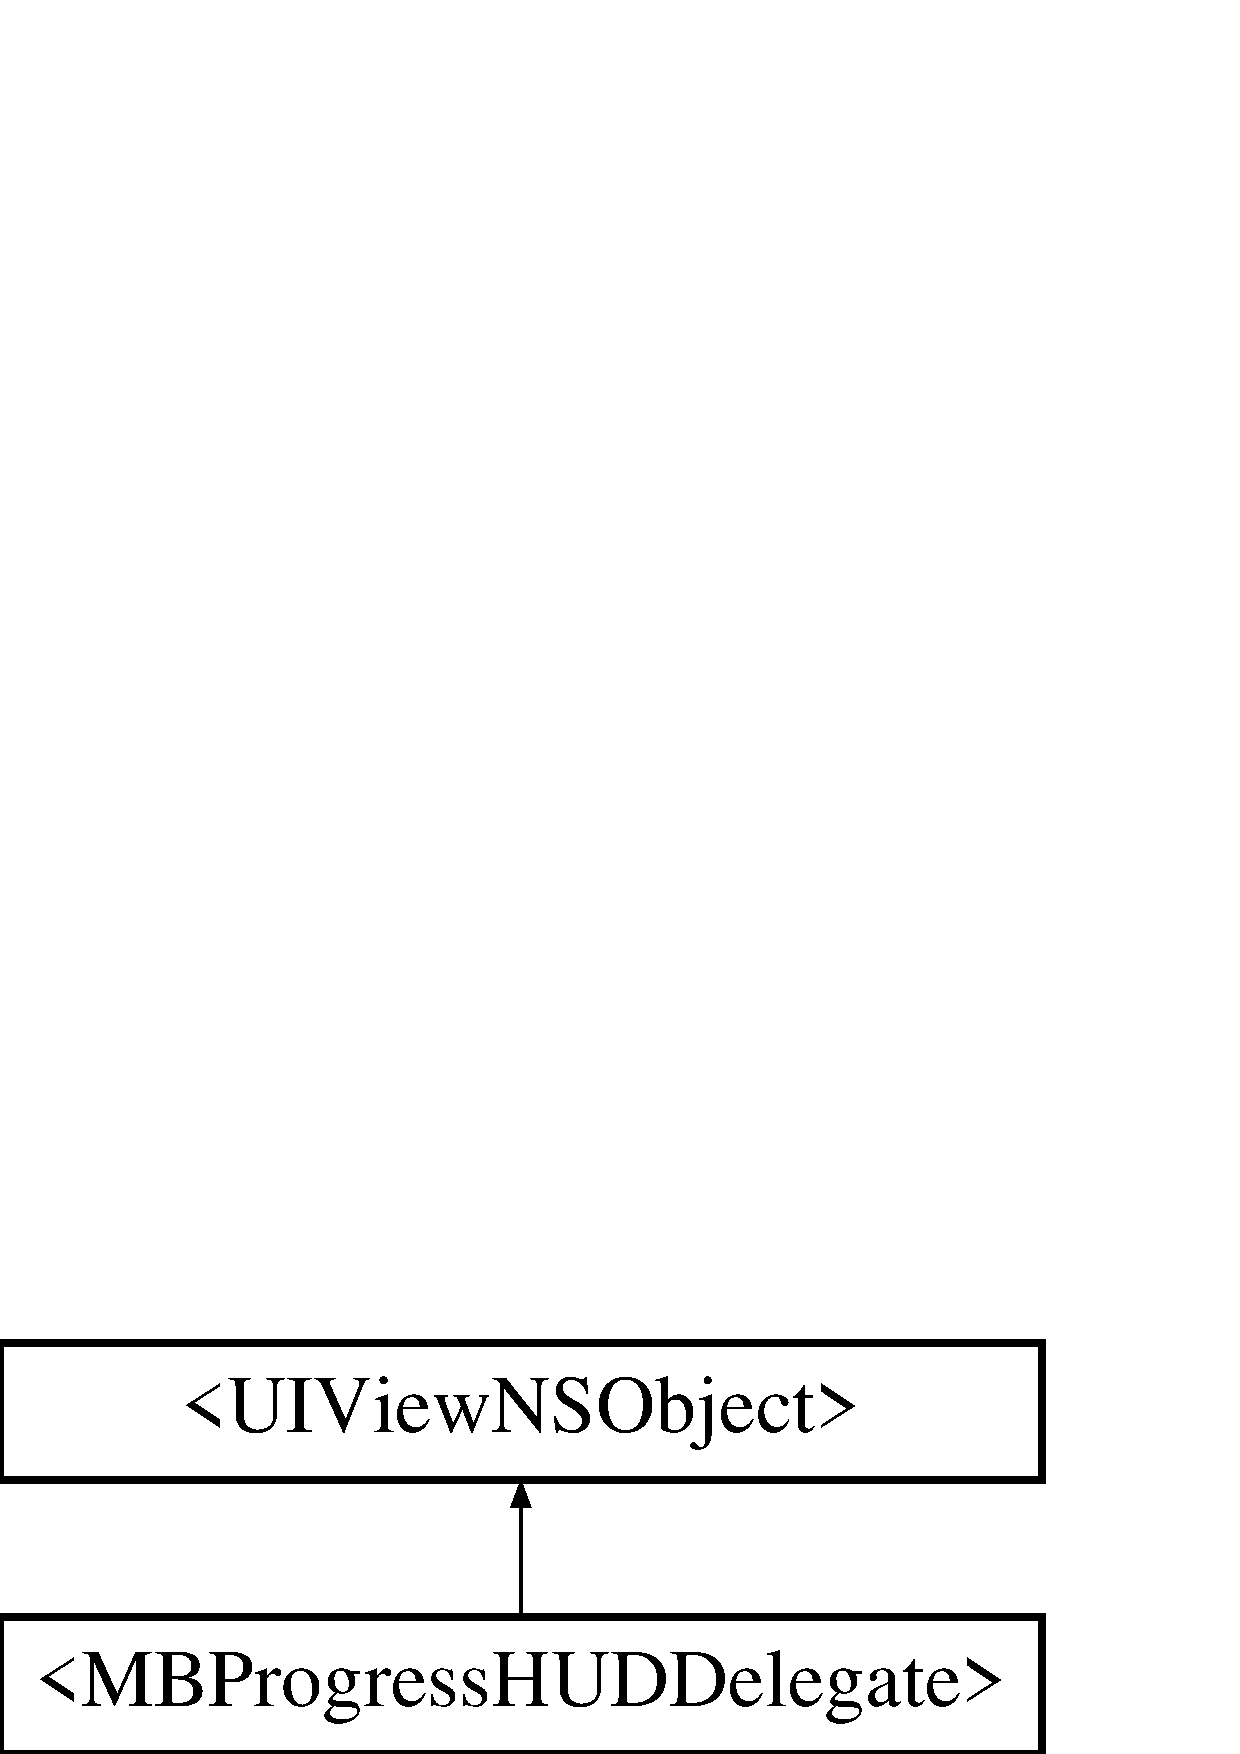
\includegraphics[height=2.000000cm]{protocol_m_b_progress_h_u_d_delegate-p}
\end{center}
\end{figure}
\subsection*{Instance Methods}
\begin{DoxyCompactItemize}
\item 
(void) -\/ \hyperlink{protocol_m_b_progress_h_u_d_delegate-p_a0b2a08b1d9cf3758cca8d52a61bed1cc}{hud\+Was\+Hidden\+:}
\end{DoxyCompactItemize}


\subsection{Detailed Description}


Definition at line 430 of file M\+B\+Progress\+H\+U\+D.\+h.



\subsection{Method Documentation}
\hypertarget{protocol_m_b_progress_h_u_d_delegate-p_a0b2a08b1d9cf3758cca8d52a61bed1cc}{\index{M\+B\+Progress\+H\+U\+D\+Delegate-\/p@{M\+B\+Progress\+H\+U\+D\+Delegate-\/p}!hud\+Was\+Hidden\+:@{hud\+Was\+Hidden\+:}}
\index{hud\+Was\+Hidden\+:@{hud\+Was\+Hidden\+:}!M\+B\+Progress\+H\+U\+D\+Delegate-\/p@{M\+B\+Progress\+H\+U\+D\+Delegate-\/p}}
\subsubsection[{hud\+Was\+Hidden\+:}]{\setlength{\rightskip}{0pt plus 5cm}-\/ (void) hud\+Was\+Hidden\+: 
\begin{DoxyParamCaption}
\item[{({\bf M\+B\+Progress\+H\+U\+D} $\ast$)}]{hud}
\end{DoxyParamCaption}
\hspace{0.3cm}{\ttfamily [optional]}}}\label{protocol_m_b_progress_h_u_d_delegate-p_a0b2a08b1d9cf3758cca8d52a61bed1cc}
Called after the H\+U\+D was fully hidden from the screen. 

The documentation for this protocol was generated from the following file\+:\begin{DoxyCompactItemize}
\item 
Utilities/\hyperlink{_m_b_progress_h_u_d_8h}{M\+B\+Progress\+H\+U\+D.\+h}\end{DoxyCompactItemize}

\hypertarget{interface_m_b_round_progress_view}{\section{M\+B\+Round\+Progress\+View Class Reference}
\label{interface_m_b_round_progress_view}\index{M\+B\+Round\+Progress\+View@{M\+B\+Round\+Progress\+View}}
}


{\ttfamily \#import $<$M\+B\+Progress\+H\+U\+D.\+h$>$}

Inheritance diagram for M\+B\+Round\+Progress\+View\+:\begin{figure}[H]
\begin{center}
\leavevmode
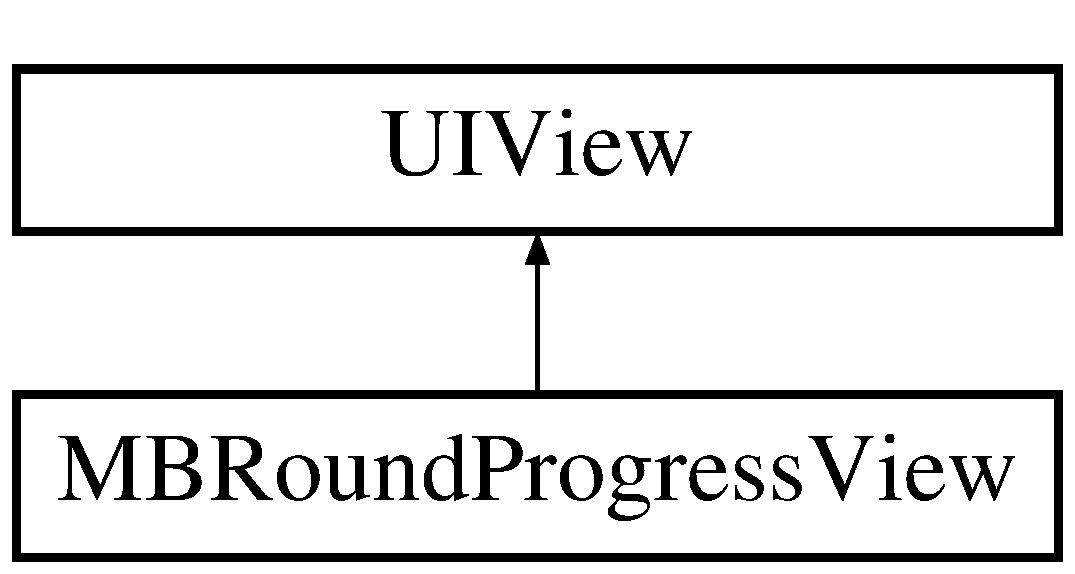
\includegraphics[height=2.000000cm]{interface_m_b_round_progress_view}
\end{center}
\end{figure}
\subsection*{Properties}
\begin{DoxyCompactItemize}
\item 
float \hyperlink{interface_m_b_round_progress_view_af92eeb35944c81f406571bc353dc5d5a}{progress}
\item 
U\+I\+Color $\ast$ \hyperlink{interface_m_b_round_progress_view_ae5c8d76a85810a3f843f262bdfff1163}{progress\+Tint\+Color}
\item 
U\+I\+Color $\ast$ \hyperlink{interface_m_b_round_progress_view_ab111d2fa027158e7c21ad411767d193a}{background\+Tint\+Color}
\item 
B\+O\+O\+L \hyperlink{interface_m_b_round_progress_view_abac11853dafb3f11426dab6d42834f9c}{annular}
\end{DoxyCompactItemize}


\subsection{Detailed Description}
A progress view for showing definite progress by filling up a circle (pie chart). 

Definition at line 445 of file M\+B\+Progress\+H\+U\+D.\+h.



\subsection{Property Documentation}
\hypertarget{interface_m_b_round_progress_view_abac11853dafb3f11426dab6d42834f9c}{\index{M\+B\+Round\+Progress\+View@{M\+B\+Round\+Progress\+View}!annular@{annular}}
\index{annular@{annular}!M\+B\+Round\+Progress\+View@{M\+B\+Round\+Progress\+View}}
\subsubsection[{annular}]{\setlength{\rightskip}{0pt plus 5cm}-\/ (B\+O\+O\+L) annular\hspace{0.3cm}{\ttfamily [read]}, {\ttfamily [write]}, {\ttfamily [nonatomic]}, {\ttfamily [assign]}}}\label{interface_m_b_round_progress_view_abac11853dafb3f11426dab6d42834f9c}


Definition at line 467 of file M\+B\+Progress\+H\+U\+D.\+h.

\hypertarget{interface_m_b_round_progress_view_ab111d2fa027158e7c21ad411767d193a}{\index{M\+B\+Round\+Progress\+View@{M\+B\+Round\+Progress\+View}!background\+Tint\+Color@{background\+Tint\+Color}}
\index{background\+Tint\+Color@{background\+Tint\+Color}!M\+B\+Round\+Progress\+View@{M\+B\+Round\+Progress\+View}}
\subsubsection[{background\+Tint\+Color}]{\setlength{\rightskip}{0pt plus 5cm}-\/ (U\+I\+Color$\ast$) background\+Tint\+Color\hspace{0.3cm}{\ttfamily [read]}, {\ttfamily [write]}, {\ttfamily [nonatomic]}, {\ttfamily [assign]}}}\label{interface_m_b_round_progress_view_ab111d2fa027158e7c21ad411767d193a}
Indicator background (non-\/progress) color. Defaults to translucent white (alpha 0.\+1) 

Definition at line 462 of file M\+B\+Progress\+H\+U\+D.\+h.

\hypertarget{interface_m_b_round_progress_view_af92eeb35944c81f406571bc353dc5d5a}{\index{M\+B\+Round\+Progress\+View@{M\+B\+Round\+Progress\+View}!progress@{progress}}
\index{progress@{progress}!M\+B\+Round\+Progress\+View@{M\+B\+Round\+Progress\+View}}
\subsubsection[{progress}]{\setlength{\rightskip}{0pt plus 5cm}-\/ (float) progress\hspace{0.3cm}{\ttfamily [read]}, {\ttfamily [write]}, {\ttfamily [nonatomic]}, {\ttfamily [assign]}}}\label{interface_m_b_round_progress_view_af92eeb35944c81f406571bc353dc5d5a}
Progress (0.\+0 to 1.\+0) 

Definition at line 450 of file M\+B\+Progress\+H\+U\+D.\+h.

\hypertarget{interface_m_b_round_progress_view_ae5c8d76a85810a3f843f262bdfff1163}{\index{M\+B\+Round\+Progress\+View@{M\+B\+Round\+Progress\+View}!progress\+Tint\+Color@{progress\+Tint\+Color}}
\index{progress\+Tint\+Color@{progress\+Tint\+Color}!M\+B\+Round\+Progress\+View@{M\+B\+Round\+Progress\+View}}
\subsubsection[{progress\+Tint\+Color}]{\setlength{\rightskip}{0pt plus 5cm}-\/ (U\+I\+Color$\ast$) progress\+Tint\+Color\hspace{0.3cm}{\ttfamily [read]}, {\ttfamily [write]}, {\ttfamily [nonatomic]}, {\ttfamily [assign]}}}\label{interface_m_b_round_progress_view_ae5c8d76a85810a3f843f262bdfff1163}
Indicator progress color. Defaults to white \mbox{[}U\+I\+Color white\+Color\mbox{]} 

Definition at line 456 of file M\+B\+Progress\+H\+U\+D.\+h.



The documentation for this class was generated from the following file\+:\begin{DoxyCompactItemize}
\item 
Misfit\+Heart\+Rate/\+Utilities/\hyperlink{_m_b_progress_h_u_d_8h}{M\+B\+Progress\+H\+U\+D.\+h}\end{DoxyCompactItemize}

\hypertarget{interface_m_h_r_app_delegate}{\section{M\+H\+R\+App\+Delegate Class Reference}
\label{interface_m_h_r_app_delegate}\index{M\+H\+R\+App\+Delegate@{M\+H\+R\+App\+Delegate}}
}


{\ttfamily \#import $<$M\+H\+R\+App\+Delegate.\+hpp$>$}

Inheritance diagram for M\+H\+R\+App\+Delegate\+:\begin{figure}[H]
\begin{center}
\leavevmode
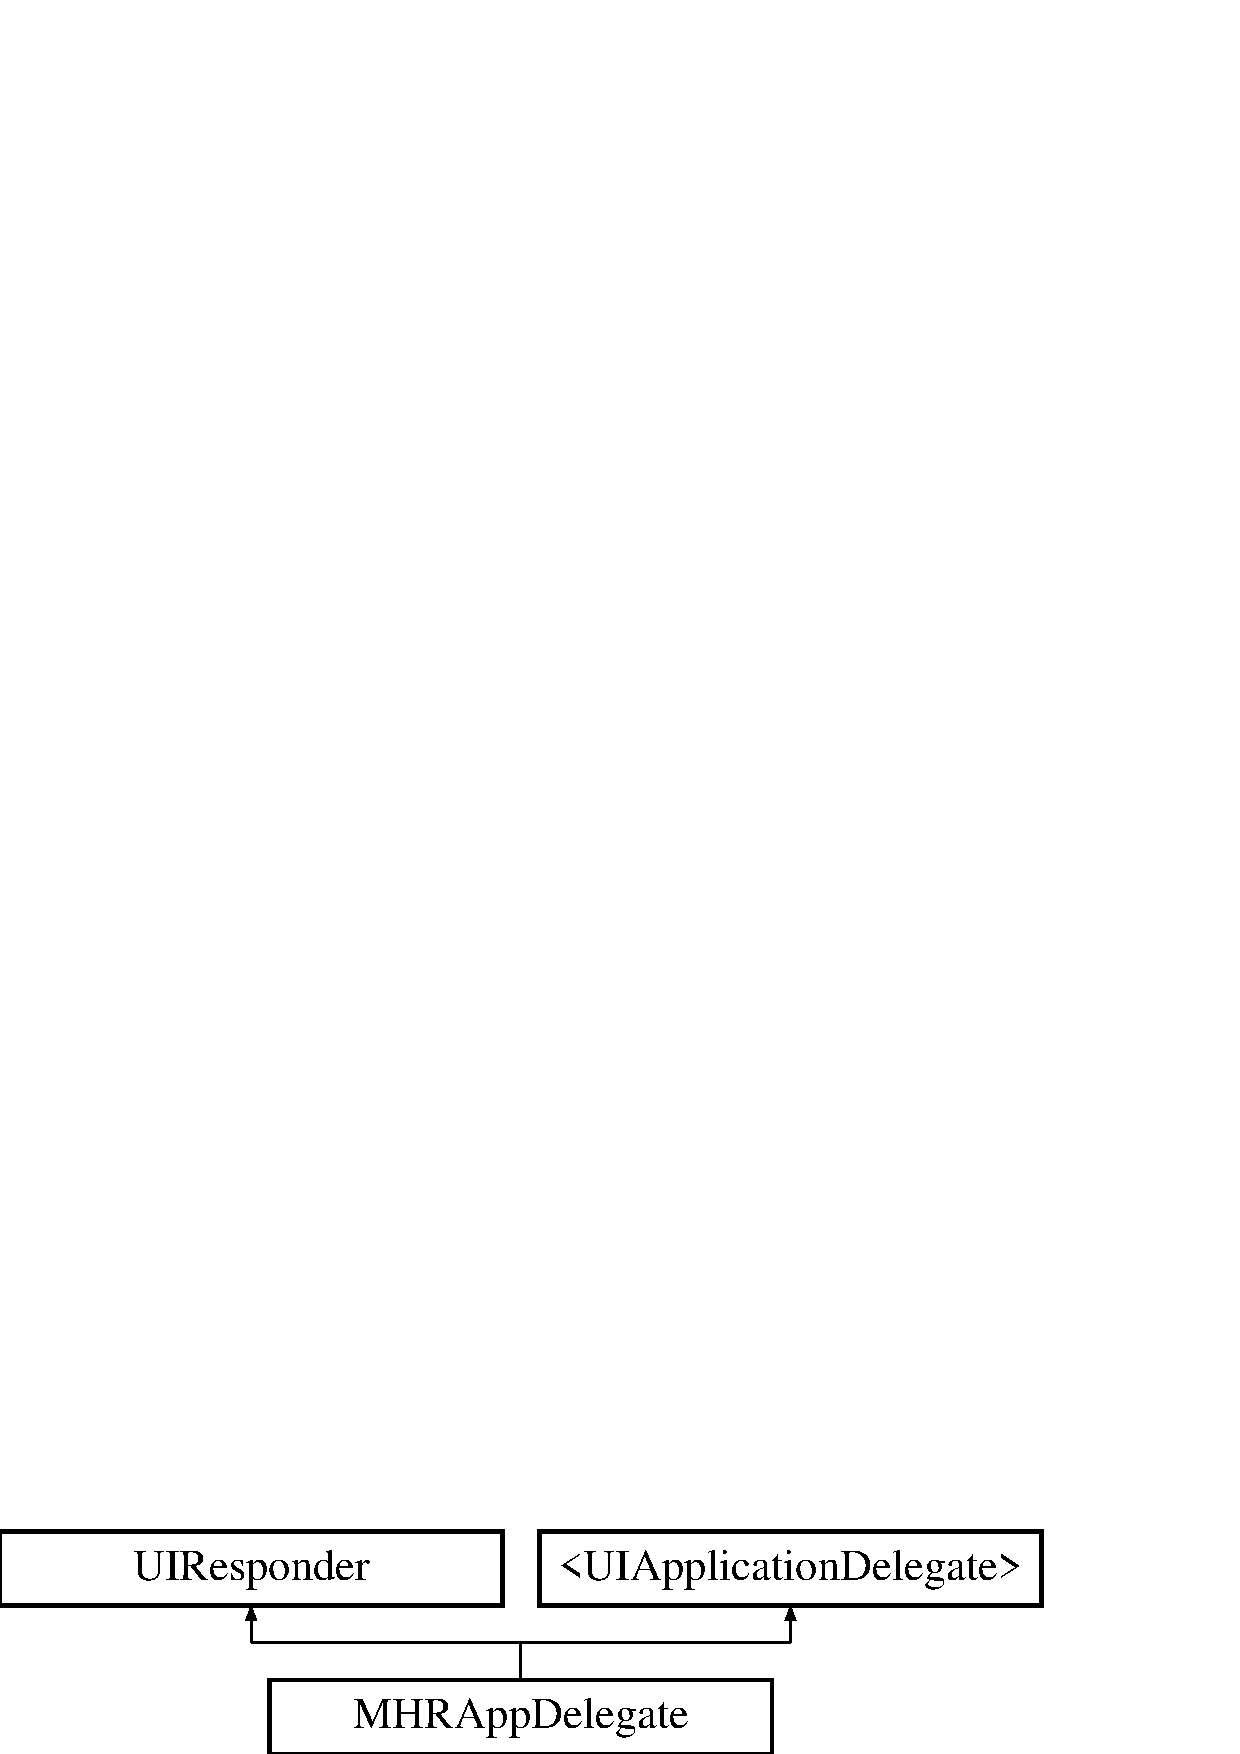
\includegraphics[height=2.000000cm]{interface_m_h_r_app_delegate}
\end{center}
\end{figure}
\subsection*{Instance Methods}
\begin{DoxyCompactItemize}
\item 
(void) -\/ \hyperlink{interface_m_h_r_app_delegate_aec18685dadaebd97aa02780c3f43c5c1}{save\+Context}
\item 
(N\+S\+U\+R\+L $\ast$) -\/ \hyperlink{interface_m_h_r_app_delegate_a7f18dc9ee3d899f8b4661b48734f1001}{application\+Documents\+Directory}
\item 
(N\+S\+Dictionary $\ast$) -\/ \hyperlink{interface_m_h_r_app_delegate_ac246805d8cd3d8477430f1a9c7fefbac}{get\+Plist\+Skin\+Dict}
\end{DoxyCompactItemize}
\subsection*{Properties}
\begin{DoxyCompactItemize}
\item 
U\+I\+Window $\ast$ \hyperlink{interface_m_h_r_app_delegate_ae07fbc2242a8ac6a6cca11d22a56dede}{window}
\item 
N\+S\+Managed\+Object\+Context $\ast$ \hyperlink{interface_m_h_r_app_delegate_a798999c986183b6b0f61070b46856713}{managed\+Object\+Context}
\item 
N\+S\+Managed\+Object\+Model $\ast$ \hyperlink{interface_m_h_r_app_delegate_ab0f79ebe18e402e0249870b98354612b}{managed\+Object\+Model}
\item 
N\+S\+Persistent\+Store\+Coordinator $\ast$ \hyperlink{interface_m_h_r_app_delegate_ade32c3c30bed3706907d1a52c129da79}{persistent\+Store\+Coordinator}
\end{DoxyCompactItemize}


\subsection{Detailed Description}


Definition at line 11 of file M\+H\+R\+App\+Delegate.\+hpp.



\subsection{Method Documentation}
\hypertarget{interface_m_h_r_app_delegate_a7f18dc9ee3d899f8b4661b48734f1001}{\index{M\+H\+R\+App\+Delegate@{M\+H\+R\+App\+Delegate}!application\+Documents\+Directory@{application\+Documents\+Directory}}
\index{application\+Documents\+Directory@{application\+Documents\+Directory}!M\+H\+R\+App\+Delegate@{M\+H\+R\+App\+Delegate}}
\subsubsection[{application\+Documents\+Directory}]{\setlength{\rightskip}{0pt plus 5cm}-\/ (N\+S\+U\+R\+L $\ast$) application\+Documents\+Directory 
\begin{DoxyParamCaption}
{}
\end{DoxyParamCaption}
}}\label{interface_m_h_r_app_delegate_a7f18dc9ee3d899f8b4661b48734f1001}


Definition at line 166 of file M\+H\+R\+App\+Delegate.\+mm.

\hypertarget{interface_m_h_r_app_delegate_ac246805d8cd3d8477430f1a9c7fefbac}{\index{M\+H\+R\+App\+Delegate@{M\+H\+R\+App\+Delegate}!get\+Plist\+Skin\+Dict@{get\+Plist\+Skin\+Dict}}
\index{get\+Plist\+Skin\+Dict@{get\+Plist\+Skin\+Dict}!M\+H\+R\+App\+Delegate@{M\+H\+R\+App\+Delegate}}
\subsubsection[{get\+Plist\+Skin\+Dict}]{\setlength{\rightskip}{0pt plus 5cm}-\/ (N\+S\+Dictionary $\ast$) get\+Plist\+Skin\+Dict 
\begin{DoxyParamCaption}
{}
\end{DoxyParamCaption}
}}\label{interface_m_h_r_app_delegate_ac246805d8cd3d8477430f1a9c7fefbac}


Definition at line 37 of file M\+H\+R\+App\+Delegate.\+mm.

\hypertarget{interface_m_h_r_app_delegate_aec18685dadaebd97aa02780c3f43c5c1}{\index{M\+H\+R\+App\+Delegate@{M\+H\+R\+App\+Delegate}!save\+Context@{save\+Context}}
\index{save\+Context@{save\+Context}!M\+H\+R\+App\+Delegate@{M\+H\+R\+App\+Delegate}}
\subsubsection[{save\+Context}]{\setlength{\rightskip}{0pt plus 5cm}-\/ (void) save\+Context 
\begin{DoxyParamCaption}
{}
\end{DoxyParamCaption}
}}\label{interface_m_h_r_app_delegate_aec18685dadaebd97aa02780c3f43c5c1}


Definition at line 76 of file M\+H\+R\+App\+Delegate.\+mm.



\subsection{Property Documentation}
\hypertarget{interface_m_h_r_app_delegate_a798999c986183b6b0f61070b46856713}{\index{M\+H\+R\+App\+Delegate@{M\+H\+R\+App\+Delegate}!managed\+Object\+Context@{managed\+Object\+Context}}
\index{managed\+Object\+Context@{managed\+Object\+Context}!M\+H\+R\+App\+Delegate@{M\+H\+R\+App\+Delegate}}
\subsubsection[{managed\+Object\+Context}]{\setlength{\rightskip}{0pt plus 5cm}-\/ (N\+S\+Managed\+Object\+Context $\ast$) managed\+Object\+Context\hspace{0.3cm}{\ttfamily [read]}, {\ttfamily [nonatomic]}, {\ttfamily [strong]}}}\label{interface_m_h_r_app_delegate_a798999c986183b6b0f61070b46856713}


Definition at line 15 of file M\+H\+R\+App\+Delegate.\+hpp.

\hypertarget{interface_m_h_r_app_delegate_ab0f79ebe18e402e0249870b98354612b}{\index{M\+H\+R\+App\+Delegate@{M\+H\+R\+App\+Delegate}!managed\+Object\+Model@{managed\+Object\+Model}}
\index{managed\+Object\+Model@{managed\+Object\+Model}!M\+H\+R\+App\+Delegate@{M\+H\+R\+App\+Delegate}}
\subsubsection[{managed\+Object\+Model}]{\setlength{\rightskip}{0pt plus 5cm}-\/ (N\+S\+Managed\+Object\+Model $\ast$) managed\+Object\+Model\hspace{0.3cm}{\ttfamily [read]}, {\ttfamily [nonatomic]}, {\ttfamily [strong]}}}\label{interface_m_h_r_app_delegate_ab0f79ebe18e402e0249870b98354612b}


Definition at line 16 of file M\+H\+R\+App\+Delegate.\+hpp.

\hypertarget{interface_m_h_r_app_delegate_ade32c3c30bed3706907d1a52c129da79}{\index{M\+H\+R\+App\+Delegate@{M\+H\+R\+App\+Delegate}!persistent\+Store\+Coordinator@{persistent\+Store\+Coordinator}}
\index{persistent\+Store\+Coordinator@{persistent\+Store\+Coordinator}!M\+H\+R\+App\+Delegate@{M\+H\+R\+App\+Delegate}}
\subsubsection[{persistent\+Store\+Coordinator}]{\setlength{\rightskip}{0pt plus 5cm}-\/ (N\+S\+Persistent\+Store\+Coordinator $\ast$) persistent\+Store\+Coordinator\hspace{0.3cm}{\ttfamily [read]}, {\ttfamily [nonatomic]}, {\ttfamily [strong]}}}\label{interface_m_h_r_app_delegate_ade32c3c30bed3706907d1a52c129da79}


Definition at line 17 of file M\+H\+R\+App\+Delegate.\+hpp.

\hypertarget{interface_m_h_r_app_delegate_ae07fbc2242a8ac6a6cca11d22a56dede}{\index{M\+H\+R\+App\+Delegate@{M\+H\+R\+App\+Delegate}!window@{window}}
\index{window@{window}!M\+H\+R\+App\+Delegate@{M\+H\+R\+App\+Delegate}}
\subsubsection[{window}]{\setlength{\rightskip}{0pt plus 5cm}-\/ (U\+I\+Window$\ast$) window\hspace{0.3cm}{\ttfamily [read]}, {\ttfamily [write]}, {\ttfamily [nonatomic]}, {\ttfamily [strong]}}}\label{interface_m_h_r_app_delegate_ae07fbc2242a8ac6a6cca11d22a56dede}


Definition at line 13 of file M\+H\+R\+App\+Delegate.\+hpp.



The documentation for this class was generated from the following files\+:\begin{DoxyCompactItemize}
\item 
Misfit\+Heart\+Rate/\hyperlink{_m_h_r_app_delegate_8hpp}{M\+H\+R\+App\+Delegate.\+hpp}\item 
Misfit\+Heart\+Rate/\hyperlink{_m_h_r_app_delegate_8mm}{M\+H\+R\+App\+Delegate.\+mm}\end{DoxyCompactItemize}

\hypertarget{interface_m_h_r_main_view_controller}{\section{M\+H\+R\+Main\+View\+Controller Class Reference}
\label{interface_m_h_r_main_view_controller}\index{M\+H\+R\+Main\+View\+Controller@{M\+H\+R\+Main\+View\+Controller}}
}


{\ttfamily \#import $<$M\+H\+R\+Main\+View\+Controller.\+hpp$>$}

Inheritance diagram for M\+H\+R\+Main\+View\+Controller\+:\begin{figure}[H]
\begin{center}
\leavevmode
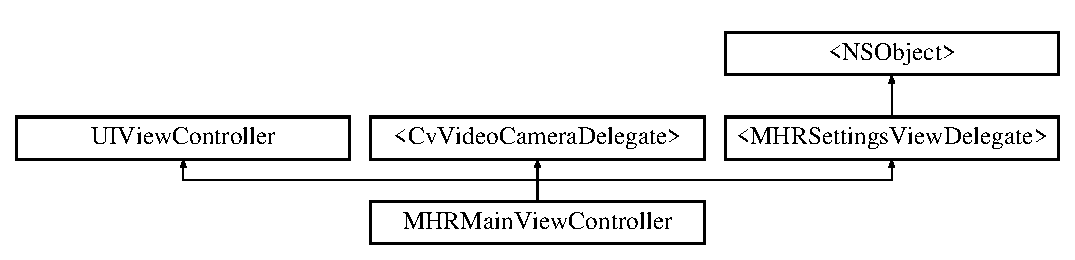
\includegraphics[height=3.000000cm]{interface_m_h_r_main_view_controller}
\end{center}
\end{figure}
\subsection*{Additional Inherited Members}


\subsection{Detailed Description}


Definition at line 31 of file M\+H\+R\+Main\+View\+Controller.\+hpp.



The documentation for this class was generated from the following file\+:\begin{DoxyCompactItemize}
\item 
Misfit\+Heart\+Rate/\+Main\+View/\hyperlink{_m_h_r_main_view_controller_8hpp}{M\+H\+R\+Main\+View\+Controller.\+hpp}\end{DoxyCompactItemize}

\hypertarget{category_m_h_r_main_view_controller_07_08}{\section{M\+H\+R\+Main\+View\+Controller() Category Reference}
\label{category_m_h_r_main_view_controller_07_08}\index{M\+H\+R\+Main\+View\+Controller()@{M\+H\+R\+Main\+View\+Controller()}}
}
\subsection*{Protected Attributes}
\begin{DoxyCompactItemize}
\item 
B\+O\+O\+L \hyperlink{category_m_h_r_main_view_controller_07_08_a0b32e144ea6d386ce5180a75b7f1ac76}{is\+Capturing}
\item 
cv\+::\+Rect \hyperlink{category_m_h_r_main_view_controller_07_08_a2508c2c272b97794449944d901733307}{crop\+Area}
\item 
cv\+::\+Rect \hyperlink{category_m_h_r_main_view_controller_07_08_a8ec78910220259631707236b9160c626}{R\+O\+I\+\_\+upper}
\item 
cv\+::\+Rect \hyperlink{category_m_h_r_main_view_controller_07_08_a8e5e7cd7481bac3b8bf77d684976a283}{R\+O\+I\+\_\+lower}
\item 
\hyperlink{interface_m_h_r_result_view_controller}{M\+H\+R\+Result\+View\+Controller} $\ast$ \hyperlink{category_m_h_r_main_view_controller_07_08_aee235ca60383f404b812a075eca55e75}{result\+View}
\item 
\hyperlink{struct_m_h_r_1_1hr_result}{hr\+Result} \hyperlink{category_m_h_r_main_view_controller_07_08_a8c4078159735c117ecbeb565b9c287e2}{current\+Result}
\item 
int \hyperlink{category_m_h_r_main_view_controller_07_08_a796178035a8c8f1b629b666076fe1ef3}{frames\+With\+Face}
\item 
int \hyperlink{category_m_h_r_main_view_controller_07_08_a7c19b115c59979a430b286b0ab7d57cc}{frames\+With\+No\+Face}
\item 
\hyperlink{interface_m_b_progress_h_u_d}{M\+B\+Progress\+H\+U\+D} $\ast$ \hyperlink{category_m_h_r_main_view_controller_07_08_ad7e9d3339af1110426f965b7615b5988}{progress\+H\+U\+D}
\item 
bool \hyperlink{category_m_h_r_main_view_controller_07_08_ade66611f85011833b732d24a430338e8}{is\+Calc\+Mode}
\item 
double \hyperlink{category_m_h_r_main_view_controller_07_08_ac4984c4b9f2c0ed7a71d957858a0b690}{lower\+\_\+range}
\item 
double \hyperlink{category_m_h_r_main_view_controller_07_08_a2cae5817c804f84f5e8db9531d8258c9}{upper\+\_\+range}
\item 
\hyperlink{struct_m_h_r_1_1hr_result}{hr\+Result} \hyperlink{category_m_h_r_main_view_controller_07_08_a9dbae9ee1ba7bf908a253626a618ecf6}{result}
\item 
std\+::vector$<$ double $>$ \hyperlink{category_m_h_r_main_view_controller_07_08_abc8096634910dfbb9d748b376d8506cb}{temporal\+\_\+mean}
\item 
N\+S\+Mutable\+Array $\ast$ \hyperlink{category_m_h_r_main_view_controller_07_08_aaf8cf1ed833d48edb06718b6d7540fae}{frame\+Index\+Array}
\item 
N\+S\+Operation\+Queue $\ast$ \hyperlink{category_m_h_r_main_view_controller_07_08_a77f4256f36d6f6bebf7f82005aec1c62}{my\+Queue}
\item 
int \hyperlink{category_m_h_r_main_view_controller_07_08_a228b693ffc5ea747c93a4206c5b8b98d}{block\+Number}
\item 
int \hyperlink{category_m_h_r_main_view_controller_07_08_a58a5e815d93639db9e1ab9f1da8fa9f9}{block\+Count}
\end{DoxyCompactItemize}
\subsection*{Properties}
\begin{DoxyCompactItemize}
\item 
Cv\+Video\+Camera $\ast$ \hyperlink{category_m_h_r_main_view_controller_07_08_a82652cbbdc0ac312a50c591870b579c1}{video\+Camera}
\item 
N\+S\+String $\ast$ \hyperlink{category_m_h_r_main_view_controller_07_08_acf930d5712d9bba15886bab49c00f36c}{out\+Path}
\item 
N\+S\+Integer \hyperlink{category_m_h_r_main_view_controller_07_08_aff8ddd68733b8b626fc832ebf2390398}{n\+Frames}
\item 
N\+S\+Integer \hyperlink{category_m_h_r_main_view_controller_07_08_ac15f6b287a439206e9a1a8816248f635}{record\+Time}
\item 
N\+S\+Timer $\ast$ \hyperlink{category_m_h_r_main_view_controller_07_08_a1f1639552968eeba13ed2b4575bea129}{record\+Timer}
\item 
I\+B\+Outlet U\+I\+Image\+View $\ast$ \hyperlink{category_m_h_r_main_view_controller_07_08_ad4a109ef255380e19bcda3c2efb2ce83}{image\+View}
\item 
I\+B\+Outlet U\+I\+Switch $\ast$ \hyperlink{category_m_h_r_main_view_controller_07_08_a64545a3386e0d53f59af539582caafd4}{camera\+Switch}
\item 
I\+B\+Outlet U\+I\+Label $\ast$ \hyperlink{category_m_h_r_main_view_controller_07_08_a2457cf5b05fac6f6cb9483997159f5f6}{face\+Label}
\item 
I\+B\+Outlet U\+I\+Label $\ast$ \hyperlink{category_m_h_r_main_view_controller_07_08_a67cd700e56983a4a3a1e6da4569bafe9}{finger\+Label}
\item 
I\+B\+Outlet U\+I\+Label $\ast$ \hyperlink{category_m_h_r_main_view_controller_07_08_a1419b93d2152551aec5038ff468f3ff6}{finger\+Switch\+Label}
\item 
I\+B\+Outlet U\+I\+Label $\ast$ \hyperlink{category_m_h_r_main_view_controller_07_08_addd32f0cbd1a4d5bfe69a837b3505ed6}{face\+Switch\+Label}
\item 
I\+B\+Outlet U\+I\+Label $\ast$ \hyperlink{category_m_h_r_main_view_controller_07_08_a63bbbfafd497288fe3035250ab5d9fcb}{record\+Time\+Label}
\item 
I\+B\+Outlet U\+I\+Bar\+Button\+Item $\ast$ \hyperlink{category_m_h_r_main_view_controller_07_08_a98273435af4fbcd1e437f257bb9ced12}{start\+Button}
\item 
I\+B\+Outlet U\+I\+Bar\+Button\+Item $\ast$ \hyperlink{category_m_h_r_main_view_controller_07_08_a0e349ec3fa2cecae6592c8d9489dedfe}{stop\+Button}
\item 
I\+B\+Outlet U\+I\+View $\ast$ \hyperlink{category_m_h_r_main_view_controller_07_08_a012367c6522cfb5d64c9d5dadcb272e2}{view\+Top}
\item 
I\+B\+Outlet U\+I\+Label $\ast$ \hyperlink{category_m_h_r_main_view_controller_07_08_a8b3917278570b1085bd6f73297f44383}{label\+Top}
\item 
I\+B\+Outlet U\+I\+View $\ast$ \hyperlink{category_m_h_r_main_view_controller_07_08_ae61668adf80d339aabb1c9dcb3085428}{view\+Top2}
\end{DoxyCompactItemize}


\subsection{Detailed Description}


Definition at line 25 of file M\+H\+R\+Main\+View\+Controller.\+mm.



\subsection{Member Data Documentation}
\hypertarget{category_m_h_r_main_view_controller_07_08_a58a5e815d93639db9e1ab9f1da8fa9f9}{\index{M\+H\+R\+Main\+View\+Controller()@{M\+H\+R\+Main\+View\+Controller()}!block\+Count@{block\+Count}}
\index{block\+Count@{block\+Count}!M\+H\+R\+Main\+View\+Controller()@{M\+H\+R\+Main\+View\+Controller()}}
\subsubsection[{block\+Count}]{\setlength{\rightskip}{0pt plus 5cm}-\/ (int) block\+Count\hspace{0.3cm}{\ttfamily [protected]}}}\label{category_m_h_r_main_view_controller_07_08_a58a5e815d93639db9e1ab9f1da8fa9f9}


Definition at line 44 of file M\+H\+R\+Main\+View\+Controller.\+mm.

\hypertarget{category_m_h_r_main_view_controller_07_08_a228b693ffc5ea747c93a4206c5b8b98d}{\index{M\+H\+R\+Main\+View\+Controller()@{M\+H\+R\+Main\+View\+Controller()}!block\+Number@{block\+Number}}
\index{block\+Number@{block\+Number}!M\+H\+R\+Main\+View\+Controller()@{M\+H\+R\+Main\+View\+Controller()}}
\subsubsection[{block\+Number}]{\setlength{\rightskip}{0pt plus 5cm}-\/ (int) block\+Number\hspace{0.3cm}{\ttfamily [protected]}}}\label{category_m_h_r_main_view_controller_07_08_a228b693ffc5ea747c93a4206c5b8b98d}


Definition at line 43 of file M\+H\+R\+Main\+View\+Controller.\+mm.

\hypertarget{category_m_h_r_main_view_controller_07_08_a2508c2c272b97794449944d901733307}{\index{M\+H\+R\+Main\+View\+Controller()@{M\+H\+R\+Main\+View\+Controller()}!crop\+Area@{crop\+Area}}
\index{crop\+Area@{crop\+Area}!M\+H\+R\+Main\+View\+Controller()@{M\+H\+R\+Main\+View\+Controller()}}
\subsubsection[{crop\+Area}]{\setlength{\rightskip}{0pt plus 5cm}-\/ (Rect {\bf M\+H\+R\+Main\+View\+Controller}())\+:\hspace{0.3cm}{\ttfamily [protected]}}}\label{category_m_h_r_main_view_controller_07_08_a2508c2c272b97794449944d901733307}


Definition at line 28 of file M\+H\+R\+Main\+View\+Controller.\+mm.

\hypertarget{category_m_h_r_main_view_controller_07_08_a8c4078159735c117ecbeb565b9c287e2}{\index{M\+H\+R\+Main\+View\+Controller()@{M\+H\+R\+Main\+View\+Controller()}!current\+Result@{current\+Result}}
\index{current\+Result@{current\+Result}!M\+H\+R\+Main\+View\+Controller()@{M\+H\+R\+Main\+View\+Controller()}}
\subsubsection[{current\+Result}]{\setlength{\rightskip}{0pt plus 5cm}-\/ ({\bf hr\+Result}) current\+Result\hspace{0.3cm}{\ttfamily [protected]}}}\label{category_m_h_r_main_view_controller_07_08_a8c4078159735c117ecbeb565b9c287e2}


Definition at line 30 of file M\+H\+R\+Main\+View\+Controller.\+mm.

\hypertarget{category_m_h_r_main_view_controller_07_08_aaf8cf1ed833d48edb06718b6d7540fae}{\index{M\+H\+R\+Main\+View\+Controller()@{M\+H\+R\+Main\+View\+Controller()}!frame\+Index\+Array@{frame\+Index\+Array}}
\index{frame\+Index\+Array@{frame\+Index\+Array}!M\+H\+R\+Main\+View\+Controller()@{M\+H\+R\+Main\+View\+Controller()}}
\subsubsection[{frame\+Index\+Array}]{\setlength{\rightskip}{0pt plus 5cm}-\/ (N\+S\+Mutable\+Array$\ast$) frame\+Index\+Array\hspace{0.3cm}{\ttfamily [protected]}}}\label{category_m_h_r_main_view_controller_07_08_aaf8cf1ed833d48edb06718b6d7540fae}


Definition at line 40 of file M\+H\+R\+Main\+View\+Controller.\+mm.

\hypertarget{category_m_h_r_main_view_controller_07_08_a796178035a8c8f1b629b666076fe1ef3}{\index{M\+H\+R\+Main\+View\+Controller()@{M\+H\+R\+Main\+View\+Controller()}!frames\+With\+Face@{frames\+With\+Face}}
\index{frames\+With\+Face@{frames\+With\+Face}!M\+H\+R\+Main\+View\+Controller()@{M\+H\+R\+Main\+View\+Controller()}}
\subsubsection[{frames\+With\+Face}]{\setlength{\rightskip}{0pt plus 5cm}-\/ (int) frames\+With\+Face\hspace{0.3cm}{\ttfamily [protected]}}}\label{category_m_h_r_main_view_controller_07_08_a796178035a8c8f1b629b666076fe1ef3}


Definition at line 31 of file M\+H\+R\+Main\+View\+Controller.\+mm.

\hypertarget{category_m_h_r_main_view_controller_07_08_a7c19b115c59979a430b286b0ab7d57cc}{\index{M\+H\+R\+Main\+View\+Controller()@{M\+H\+R\+Main\+View\+Controller()}!frames\+With\+No\+Face@{frames\+With\+No\+Face}}
\index{frames\+With\+No\+Face@{frames\+With\+No\+Face}!M\+H\+R\+Main\+View\+Controller()@{M\+H\+R\+Main\+View\+Controller()}}
\subsubsection[{frames\+With\+No\+Face}]{\setlength{\rightskip}{0pt plus 5cm}-\/ (int) frames\+With\+No\+Face\hspace{0.3cm}{\ttfamily [protected]}}}\label{category_m_h_r_main_view_controller_07_08_a7c19b115c59979a430b286b0ab7d57cc}


Definition at line 32 of file M\+H\+R\+Main\+View\+Controller.\+mm.

\hypertarget{category_m_h_r_main_view_controller_07_08_ade66611f85011833b732d24a430338e8}{\index{M\+H\+R\+Main\+View\+Controller()@{M\+H\+R\+Main\+View\+Controller()}!is\+Calc\+Mode@{is\+Calc\+Mode}}
\index{is\+Calc\+Mode@{is\+Calc\+Mode}!M\+H\+R\+Main\+View\+Controller()@{M\+H\+R\+Main\+View\+Controller()}}
\subsubsection[{is\+Calc\+Mode}]{\setlength{\rightskip}{0pt plus 5cm}-\/ (bool) is\+Calc\+Mode\hspace{0.3cm}{\ttfamily [protected]}}}\label{category_m_h_r_main_view_controller_07_08_ade66611f85011833b732d24a430338e8}


Definition at line 35 of file M\+H\+R\+Main\+View\+Controller.\+mm.

\hypertarget{category_m_h_r_main_view_controller_07_08_a0b32e144ea6d386ce5180a75b7f1ac76}{\index{M\+H\+R\+Main\+View\+Controller()@{M\+H\+R\+Main\+View\+Controller()}!is\+Capturing@{is\+Capturing}}
\index{is\+Capturing@{is\+Capturing}!M\+H\+R\+Main\+View\+Controller()@{M\+H\+R\+Main\+View\+Controller()}}
\subsubsection[{is\+Capturing}]{\setlength{\rightskip}{0pt plus 5cm}-\/ (B\+O\+O\+L) is\+Capturing\hspace{0.3cm}{\ttfamily [protected]}}}\label{category_m_h_r_main_view_controller_07_08_a0b32e144ea6d386ce5180a75b7f1ac76}


Definition at line 27 of file M\+H\+R\+Main\+View\+Controller.\+mm.

\hypertarget{category_m_h_r_main_view_controller_07_08_ac4984c4b9f2c0ed7a71d957858a0b690}{\index{M\+H\+R\+Main\+View\+Controller()@{M\+H\+R\+Main\+View\+Controller()}!lower\+\_\+range@{lower\+\_\+range}}
\index{lower\+\_\+range@{lower\+\_\+range}!M\+H\+R\+Main\+View\+Controller()@{M\+H\+R\+Main\+View\+Controller()}}
\subsubsection[{lower\+\_\+range}]{\setlength{\rightskip}{0pt plus 5cm}-\/ (double) lower\+\_\+range\hspace{0.3cm}{\ttfamily [protected]}}}\label{category_m_h_r_main_view_controller_07_08_ac4984c4b9f2c0ed7a71d957858a0b690}


Definition at line 36 of file M\+H\+R\+Main\+View\+Controller.\+mm.

\hypertarget{category_m_h_r_main_view_controller_07_08_a77f4256f36d6f6bebf7f82005aec1c62}{\index{M\+H\+R\+Main\+View\+Controller()@{M\+H\+R\+Main\+View\+Controller()}!my\+Queue@{my\+Queue}}
\index{my\+Queue@{my\+Queue}!M\+H\+R\+Main\+View\+Controller()@{M\+H\+R\+Main\+View\+Controller()}}
\subsubsection[{my\+Queue}]{\setlength{\rightskip}{0pt plus 5cm}-\/ (N\+S\+Operation\+Queue$\ast$) my\+Queue\hspace{0.3cm}{\ttfamily [protected]}}}\label{category_m_h_r_main_view_controller_07_08_a77f4256f36d6f6bebf7f82005aec1c62}


Definition at line 42 of file M\+H\+R\+Main\+View\+Controller.\+mm.

\hypertarget{category_m_h_r_main_view_controller_07_08_ad7e9d3339af1110426f965b7615b5988}{\index{M\+H\+R\+Main\+View\+Controller()@{M\+H\+R\+Main\+View\+Controller()}!progress\+H\+U\+D@{progress\+H\+U\+D}}
\index{progress\+H\+U\+D@{progress\+H\+U\+D}!M\+H\+R\+Main\+View\+Controller()@{M\+H\+R\+Main\+View\+Controller()}}
\subsubsection[{progress\+H\+U\+D}]{\setlength{\rightskip}{0pt plus 5cm}-\/ ({\bf M\+B\+Progress\+H\+U\+D}$\ast$) progress\+H\+U\+D\hspace{0.3cm}{\ttfamily [protected]}}}\label{category_m_h_r_main_view_controller_07_08_ad7e9d3339af1110426f965b7615b5988}


Definition at line 33 of file M\+H\+R\+Main\+View\+Controller.\+mm.

\hypertarget{category_m_h_r_main_view_controller_07_08_a9dbae9ee1ba7bf908a253626a618ecf6}{\index{M\+H\+R\+Main\+View\+Controller()@{M\+H\+R\+Main\+View\+Controller()}!result@{result}}
\index{result@{result}!M\+H\+R\+Main\+View\+Controller()@{M\+H\+R\+Main\+View\+Controller()}}
\subsubsection[{result}]{\setlength{\rightskip}{0pt plus 5cm}-\/ ({\bf hr\+Result}) result\hspace{0.3cm}{\ttfamily [protected]}}}\label{category_m_h_r_main_view_controller_07_08_a9dbae9ee1ba7bf908a253626a618ecf6}


Definition at line 38 of file M\+H\+R\+Main\+View\+Controller.\+mm.

\hypertarget{category_m_h_r_main_view_controller_07_08_aee235ca60383f404b812a075eca55e75}{\index{M\+H\+R\+Main\+View\+Controller()@{M\+H\+R\+Main\+View\+Controller()}!result\+View@{result\+View}}
\index{result\+View@{result\+View}!M\+H\+R\+Main\+View\+Controller()@{M\+H\+R\+Main\+View\+Controller()}}
\subsubsection[{result\+View}]{\setlength{\rightskip}{0pt plus 5cm}-\/ ({\bf M\+H\+R\+Result\+View\+Controller}$\ast$) result\+View\hspace{0.3cm}{\ttfamily [protected]}}}\label{category_m_h_r_main_view_controller_07_08_aee235ca60383f404b812a075eca55e75}


Definition at line 29 of file M\+H\+R\+Main\+View\+Controller.\+mm.

\hypertarget{category_m_h_r_main_view_controller_07_08_a8e5e7cd7481bac3b8bf77d684976a283}{\index{M\+H\+R\+Main\+View\+Controller()@{M\+H\+R\+Main\+View\+Controller()}!R\+O\+I\+\_\+lower@{R\+O\+I\+\_\+lower}}
\index{R\+O\+I\+\_\+lower@{R\+O\+I\+\_\+lower}!M\+H\+R\+Main\+View\+Controller()@{M\+H\+R\+Main\+View\+Controller()}}
\subsubsection[{R\+O\+I\+\_\+lower}]{\setlength{\rightskip}{0pt plus 5cm}-\/ (Rect {\bf M\+H\+R\+Main\+View\+Controller}())\+:\hspace{0.3cm}{\ttfamily [protected]}}}\label{category_m_h_r_main_view_controller_07_08_a8e5e7cd7481bac3b8bf77d684976a283}


Definition at line 28 of file M\+H\+R\+Main\+View\+Controller.\+mm.

\hypertarget{category_m_h_r_main_view_controller_07_08_a8ec78910220259631707236b9160c626}{\index{M\+H\+R\+Main\+View\+Controller()@{M\+H\+R\+Main\+View\+Controller()}!R\+O\+I\+\_\+upper@{R\+O\+I\+\_\+upper}}
\index{R\+O\+I\+\_\+upper@{R\+O\+I\+\_\+upper}!M\+H\+R\+Main\+View\+Controller()@{M\+H\+R\+Main\+View\+Controller()}}
\subsubsection[{R\+O\+I\+\_\+upper}]{\setlength{\rightskip}{0pt plus 5cm}-\/ (Rect {\bf M\+H\+R\+Main\+View\+Controller}())\+:\hspace{0.3cm}{\ttfamily [protected]}}}\label{category_m_h_r_main_view_controller_07_08_a8ec78910220259631707236b9160c626}


Definition at line 28 of file M\+H\+R\+Main\+View\+Controller.\+mm.

\hypertarget{category_m_h_r_main_view_controller_07_08_abc8096634910dfbb9d748b376d8506cb}{\index{M\+H\+R\+Main\+View\+Controller()@{M\+H\+R\+Main\+View\+Controller()}!temporal\+\_\+mean@{temporal\+\_\+mean}}
\index{temporal\+\_\+mean@{temporal\+\_\+mean}!M\+H\+R\+Main\+View\+Controller()@{M\+H\+R\+Main\+View\+Controller()}}
\subsubsection[{temporal\+\_\+mean}]{\setlength{\rightskip}{0pt plus 5cm}-\/ (vector$<$double$>$ {\bf M\+H\+R\+Main\+View\+Controller}())\+:\hspace{0.3cm}{\ttfamily [protected]}}}\label{category_m_h_r_main_view_controller_07_08_abc8096634910dfbb9d748b376d8506cb}


Definition at line 39 of file M\+H\+R\+Main\+View\+Controller.\+mm.

\hypertarget{category_m_h_r_main_view_controller_07_08_a2cae5817c804f84f5e8db9531d8258c9}{\index{M\+H\+R\+Main\+View\+Controller()@{M\+H\+R\+Main\+View\+Controller()}!upper\+\_\+range@{upper\+\_\+range}}
\index{upper\+\_\+range@{upper\+\_\+range}!M\+H\+R\+Main\+View\+Controller()@{M\+H\+R\+Main\+View\+Controller()}}
\subsubsection[{upper\+\_\+range}]{\setlength{\rightskip}{0pt plus 5cm}-\/ (double) upper\+\_\+range\hspace{0.3cm}{\ttfamily [protected]}}}\label{category_m_h_r_main_view_controller_07_08_a2cae5817c804f84f5e8db9531d8258c9}


Definition at line 37 of file M\+H\+R\+Main\+View\+Controller.\+mm.



\subsection{Property Documentation}
\hypertarget{category_m_h_r_main_view_controller_07_08_a64545a3386e0d53f59af539582caafd4}{\index{M\+H\+R\+Main\+View\+Controller()@{M\+H\+R\+Main\+View\+Controller()}!camera\+Switch@{camera\+Switch}}
\index{camera\+Switch@{camera\+Switch}!M\+H\+R\+Main\+View\+Controller()@{M\+H\+R\+Main\+View\+Controller()}}
\subsubsection[{camera\+Switch}]{\setlength{\rightskip}{0pt plus 5cm}-\/ (I\+B\+Outlet U\+I\+Switch$\ast$) camera\+Switch\hspace{0.3cm}{\ttfamily [read]}, {\ttfamily [write]}, {\ttfamily [nonatomic]}, {\ttfamily [weak]}}}\label{category_m_h_r_main_view_controller_07_08_a64545a3386e0d53f59af539582caafd4}


Definition at line 54 of file M\+H\+R\+Main\+View\+Controller.\+mm.

\hypertarget{category_m_h_r_main_view_controller_07_08_a2457cf5b05fac6f6cb9483997159f5f6}{\index{M\+H\+R\+Main\+View\+Controller()@{M\+H\+R\+Main\+View\+Controller()}!face\+Label@{face\+Label}}
\index{face\+Label@{face\+Label}!M\+H\+R\+Main\+View\+Controller()@{M\+H\+R\+Main\+View\+Controller()}}
\subsubsection[{face\+Label}]{\setlength{\rightskip}{0pt plus 5cm}-\/ (I\+B\+Outlet U\+I\+Label$\ast$) face\+Label\hspace{0.3cm}{\ttfamily [read]}, {\ttfamily [write]}, {\ttfamily [nonatomic]}, {\ttfamily [weak]}}}\label{category_m_h_r_main_view_controller_07_08_a2457cf5b05fac6f6cb9483997159f5f6}


Definition at line 55 of file M\+H\+R\+Main\+View\+Controller.\+mm.

\hypertarget{category_m_h_r_main_view_controller_07_08_addd32f0cbd1a4d5bfe69a837b3505ed6}{\index{M\+H\+R\+Main\+View\+Controller()@{M\+H\+R\+Main\+View\+Controller()}!face\+Switch\+Label@{face\+Switch\+Label}}
\index{face\+Switch\+Label@{face\+Switch\+Label}!M\+H\+R\+Main\+View\+Controller()@{M\+H\+R\+Main\+View\+Controller()}}
\subsubsection[{face\+Switch\+Label}]{\setlength{\rightskip}{0pt plus 5cm}-\/ (I\+B\+Outlet U\+I\+Label$\ast$) face\+Switch\+Label\hspace{0.3cm}{\ttfamily [read]}, {\ttfamily [write]}, {\ttfamily [nonatomic]}, {\ttfamily [weak]}}}\label{category_m_h_r_main_view_controller_07_08_addd32f0cbd1a4d5bfe69a837b3505ed6}


Definition at line 58 of file M\+H\+R\+Main\+View\+Controller.\+mm.

\hypertarget{category_m_h_r_main_view_controller_07_08_a67cd700e56983a4a3a1e6da4569bafe9}{\index{M\+H\+R\+Main\+View\+Controller()@{M\+H\+R\+Main\+View\+Controller()}!finger\+Label@{finger\+Label}}
\index{finger\+Label@{finger\+Label}!M\+H\+R\+Main\+View\+Controller()@{M\+H\+R\+Main\+View\+Controller()}}
\subsubsection[{finger\+Label}]{\setlength{\rightskip}{0pt plus 5cm}-\/ (I\+B\+Outlet U\+I\+Label$\ast$) finger\+Label\hspace{0.3cm}{\ttfamily [read]}, {\ttfamily [write]}, {\ttfamily [nonatomic]}, {\ttfamily [weak]}}}\label{category_m_h_r_main_view_controller_07_08_a67cd700e56983a4a3a1e6da4569bafe9}


Definition at line 56 of file M\+H\+R\+Main\+View\+Controller.\+mm.

\hypertarget{category_m_h_r_main_view_controller_07_08_a1419b93d2152551aec5038ff468f3ff6}{\index{M\+H\+R\+Main\+View\+Controller()@{M\+H\+R\+Main\+View\+Controller()}!finger\+Switch\+Label@{finger\+Switch\+Label}}
\index{finger\+Switch\+Label@{finger\+Switch\+Label}!M\+H\+R\+Main\+View\+Controller()@{M\+H\+R\+Main\+View\+Controller()}}
\subsubsection[{finger\+Switch\+Label}]{\setlength{\rightskip}{0pt plus 5cm}-\/ (I\+B\+Outlet U\+I\+Label$\ast$) finger\+Switch\+Label\hspace{0.3cm}{\ttfamily [read]}, {\ttfamily [write]}, {\ttfamily [nonatomic]}, {\ttfamily [weak]}}}\label{category_m_h_r_main_view_controller_07_08_a1419b93d2152551aec5038ff468f3ff6}


Definition at line 57 of file M\+H\+R\+Main\+View\+Controller.\+mm.

\hypertarget{category_m_h_r_main_view_controller_07_08_ad4a109ef255380e19bcda3c2efb2ce83}{\index{M\+H\+R\+Main\+View\+Controller()@{M\+H\+R\+Main\+View\+Controller()}!image\+View@{image\+View}}
\index{image\+View@{image\+View}!M\+H\+R\+Main\+View\+Controller()@{M\+H\+R\+Main\+View\+Controller()}}
\subsubsection[{image\+View}]{\setlength{\rightskip}{0pt plus 5cm}-\/ (I\+B\+Outlet U\+I\+Image\+View$\ast$) image\+View\hspace{0.3cm}{\ttfamily [read]}, {\ttfamily [write]}, {\ttfamily [nonatomic]}, {\ttfamily [weak]}}}\label{category_m_h_r_main_view_controller_07_08_ad4a109ef255380e19bcda3c2efb2ce83}


Definition at line 53 of file M\+H\+R\+Main\+View\+Controller.\+mm.

\hypertarget{category_m_h_r_main_view_controller_07_08_a8b3917278570b1085bd6f73297f44383}{\index{M\+H\+R\+Main\+View\+Controller()@{M\+H\+R\+Main\+View\+Controller()}!label\+Top@{label\+Top}}
\index{label\+Top@{label\+Top}!M\+H\+R\+Main\+View\+Controller()@{M\+H\+R\+Main\+View\+Controller()}}
\subsubsection[{label\+Top}]{\setlength{\rightskip}{0pt plus 5cm}-\/ (I\+B\+Outlet U\+I\+Label$\ast$) label\+Top\hspace{0.3cm}{\ttfamily [read]}, {\ttfamily [write]}, {\ttfamily [nonatomic]}, {\ttfamily [weak]}}}\label{category_m_h_r_main_view_controller_07_08_a8b3917278570b1085bd6f73297f44383}


Definition at line 63 of file M\+H\+R\+Main\+View\+Controller.\+mm.

\hypertarget{category_m_h_r_main_view_controller_07_08_aff8ddd68733b8b626fc832ebf2390398}{\index{M\+H\+R\+Main\+View\+Controller()@{M\+H\+R\+Main\+View\+Controller()}!n\+Frames@{n\+Frames}}
\index{n\+Frames@{n\+Frames}!M\+H\+R\+Main\+View\+Controller()@{M\+H\+R\+Main\+View\+Controller()}}
\subsubsection[{n\+Frames}]{\setlength{\rightskip}{0pt plus 5cm}-\/ (N\+S\+Integer) n\+Frames\hspace{0.3cm}{\ttfamily [read]}, {\ttfamily [write]}, {\ttfamily [nonatomic]}, {\ttfamily [assign]}}}\label{category_m_h_r_main_view_controller_07_08_aff8ddd68733b8b626fc832ebf2390398}


Definition at line 49 of file M\+H\+R\+Main\+View\+Controller.\+mm.

\hypertarget{category_m_h_r_main_view_controller_07_08_acf930d5712d9bba15886bab49c00f36c}{\index{M\+H\+R\+Main\+View\+Controller()@{M\+H\+R\+Main\+View\+Controller()}!out\+Path@{out\+Path}}
\index{out\+Path@{out\+Path}!M\+H\+R\+Main\+View\+Controller()@{M\+H\+R\+Main\+View\+Controller()}}
\subsubsection[{out\+Path}]{\setlength{\rightskip}{0pt plus 5cm}-\/ (N\+S\+String$\ast$) out\+Path\hspace{0.3cm}{\ttfamily [read]}, {\ttfamily [write]}, {\ttfamily [nonatomic]}, {\ttfamily [strong]}}}\label{category_m_h_r_main_view_controller_07_08_acf930d5712d9bba15886bab49c00f36c}


Definition at line 48 of file M\+H\+R\+Main\+View\+Controller.\+mm.

\hypertarget{category_m_h_r_main_view_controller_07_08_ac15f6b287a439206e9a1a8816248f635}{\index{M\+H\+R\+Main\+View\+Controller()@{M\+H\+R\+Main\+View\+Controller()}!record\+Time@{record\+Time}}
\index{record\+Time@{record\+Time}!M\+H\+R\+Main\+View\+Controller()@{M\+H\+R\+Main\+View\+Controller()}}
\subsubsection[{record\+Time}]{\setlength{\rightskip}{0pt plus 5cm}-\/ (N\+S\+Integer) record\+Time\hspace{0.3cm}{\ttfamily [read]}, {\ttfamily [write]}, {\ttfamily [nonatomic]}, {\ttfamily [assign]}}}\label{category_m_h_r_main_view_controller_07_08_ac15f6b287a439206e9a1a8816248f635}


Definition at line 50 of file M\+H\+R\+Main\+View\+Controller.\+mm.

\hypertarget{category_m_h_r_main_view_controller_07_08_a63bbbfafd497288fe3035250ab5d9fcb}{\index{M\+H\+R\+Main\+View\+Controller()@{M\+H\+R\+Main\+View\+Controller()}!record\+Time\+Label@{record\+Time\+Label}}
\index{record\+Time\+Label@{record\+Time\+Label}!M\+H\+R\+Main\+View\+Controller()@{M\+H\+R\+Main\+View\+Controller()}}
\subsubsection[{record\+Time\+Label}]{\setlength{\rightskip}{0pt plus 5cm}-\/ (I\+B\+Outlet U\+I\+Label$\ast$) record\+Time\+Label\hspace{0.3cm}{\ttfamily [read]}, {\ttfamily [write]}, {\ttfamily [nonatomic]}, {\ttfamily [weak]}}}\label{category_m_h_r_main_view_controller_07_08_a63bbbfafd497288fe3035250ab5d9fcb}


Definition at line 59 of file M\+H\+R\+Main\+View\+Controller.\+mm.

\hypertarget{category_m_h_r_main_view_controller_07_08_a1f1639552968eeba13ed2b4575bea129}{\index{M\+H\+R\+Main\+View\+Controller()@{M\+H\+R\+Main\+View\+Controller()}!record\+Timer@{record\+Timer}}
\index{record\+Timer@{record\+Timer}!M\+H\+R\+Main\+View\+Controller()@{M\+H\+R\+Main\+View\+Controller()}}
\subsubsection[{record\+Timer}]{\setlength{\rightskip}{0pt plus 5cm}-\/ (N\+S\+Timer$\ast$) record\+Timer\hspace{0.3cm}{\ttfamily [read]}, {\ttfamily [write]}, {\ttfamily [nonatomic]}, {\ttfamily [strong]}}}\label{category_m_h_r_main_view_controller_07_08_a1f1639552968eeba13ed2b4575bea129}


Definition at line 51 of file M\+H\+R\+Main\+View\+Controller.\+mm.

\hypertarget{category_m_h_r_main_view_controller_07_08_a98273435af4fbcd1e437f257bb9ced12}{\index{M\+H\+R\+Main\+View\+Controller()@{M\+H\+R\+Main\+View\+Controller()}!start\+Button@{start\+Button}}
\index{start\+Button@{start\+Button}!M\+H\+R\+Main\+View\+Controller()@{M\+H\+R\+Main\+View\+Controller()}}
\subsubsection[{start\+Button}]{\setlength{\rightskip}{0pt plus 5cm}-\/ (I\+B\+Outlet U\+I\+Bar\+Button\+Item$\ast$) start\+Button\hspace{0.3cm}{\ttfamily [read]}, {\ttfamily [write]}, {\ttfamily [nonatomic]}, {\ttfamily [strong]}}}\label{category_m_h_r_main_view_controller_07_08_a98273435af4fbcd1e437f257bb9ced12}


Definition at line 60 of file M\+H\+R\+Main\+View\+Controller.\+mm.

\hypertarget{category_m_h_r_main_view_controller_07_08_a0e349ec3fa2cecae6592c8d9489dedfe}{\index{M\+H\+R\+Main\+View\+Controller()@{M\+H\+R\+Main\+View\+Controller()}!stop\+Button@{stop\+Button}}
\index{stop\+Button@{stop\+Button}!M\+H\+R\+Main\+View\+Controller()@{M\+H\+R\+Main\+View\+Controller()}}
\subsubsection[{stop\+Button}]{\setlength{\rightskip}{0pt plus 5cm}-\/ (I\+B\+Outlet U\+I\+Bar\+Button\+Item$\ast$) stop\+Button\hspace{0.3cm}{\ttfamily [read]}, {\ttfamily [write]}, {\ttfamily [nonatomic]}, {\ttfamily [strong]}}}\label{category_m_h_r_main_view_controller_07_08_a0e349ec3fa2cecae6592c8d9489dedfe}


Definition at line 61 of file M\+H\+R\+Main\+View\+Controller.\+mm.

\hypertarget{category_m_h_r_main_view_controller_07_08_a82652cbbdc0ac312a50c591870b579c1}{\index{M\+H\+R\+Main\+View\+Controller()@{M\+H\+R\+Main\+View\+Controller()}!video\+Camera@{video\+Camera}}
\index{video\+Camera@{video\+Camera}!M\+H\+R\+Main\+View\+Controller()@{M\+H\+R\+Main\+View\+Controller()}}
\subsubsection[{video\+Camera}]{\setlength{\rightskip}{0pt plus 5cm}-\/ (Cv\+Video\+Camera$\ast$) video\+Camera\hspace{0.3cm}{\ttfamily [read]}, {\ttfamily [write]}, {\ttfamily [nonatomic]}, {\ttfamily [retain]}}}\label{category_m_h_r_main_view_controller_07_08_a82652cbbdc0ac312a50c591870b579c1}


Definition at line 47 of file M\+H\+R\+Main\+View\+Controller.\+mm.

\hypertarget{category_m_h_r_main_view_controller_07_08_a012367c6522cfb5d64c9d5dadcb272e2}{\index{M\+H\+R\+Main\+View\+Controller()@{M\+H\+R\+Main\+View\+Controller()}!view\+Top@{view\+Top}}
\index{view\+Top@{view\+Top}!M\+H\+R\+Main\+View\+Controller()@{M\+H\+R\+Main\+View\+Controller()}}
\subsubsection[{view\+Top}]{\setlength{\rightskip}{0pt plus 5cm}-\/ (I\+B\+Outlet U\+I\+View$\ast$) view\+Top\hspace{0.3cm}{\ttfamily [read]}, {\ttfamily [write]}, {\ttfamily [nonatomic]}, {\ttfamily [weak]}}}\label{category_m_h_r_main_view_controller_07_08_a012367c6522cfb5d64c9d5dadcb272e2}


Definition at line 62 of file M\+H\+R\+Main\+View\+Controller.\+mm.

\hypertarget{category_m_h_r_main_view_controller_07_08_ae61668adf80d339aabb1c9dcb3085428}{\index{M\+H\+R\+Main\+View\+Controller()@{M\+H\+R\+Main\+View\+Controller()}!view\+Top2@{view\+Top2}}
\index{view\+Top2@{view\+Top2}!M\+H\+R\+Main\+View\+Controller()@{M\+H\+R\+Main\+View\+Controller()}}
\subsubsection[{view\+Top2}]{\setlength{\rightskip}{0pt plus 5cm}-\/ (I\+B\+Outlet U\+I\+View$\ast$) view\+Top2\hspace{0.3cm}{\ttfamily [read]}, {\ttfamily [write]}, {\ttfamily [nonatomic]}, {\ttfamily [weak]}}}\label{category_m_h_r_main_view_controller_07_08_ae61668adf80d339aabb1c9dcb3085428}


Definition at line 64 of file M\+H\+R\+Main\+View\+Controller.\+mm.



The documentation for this category was generated from the following file\+:\begin{DoxyCompactItemize}
\item 
Main\+View/\hyperlink{_m_h_r_main_view_controller_8mm}{M\+H\+R\+Main\+View\+Controller.\+mm}\end{DoxyCompactItemize}

\hypertarget{interface_m_h_r_result_view_controller}{\section{M\+H\+R\+Result\+View\+Controller Class Reference}
\label{interface_m_h_r_result_view_controller}\index{M\+H\+R\+Result\+View\+Controller@{M\+H\+R\+Result\+View\+Controller}}
}


{\ttfamily \#import $<$M\+H\+R\+Result\+View\+Controller.\+hpp$>$}

Inheritance diagram for M\+H\+R\+Result\+View\+Controller\+:\begin{figure}[H]
\begin{center}
\leavevmode
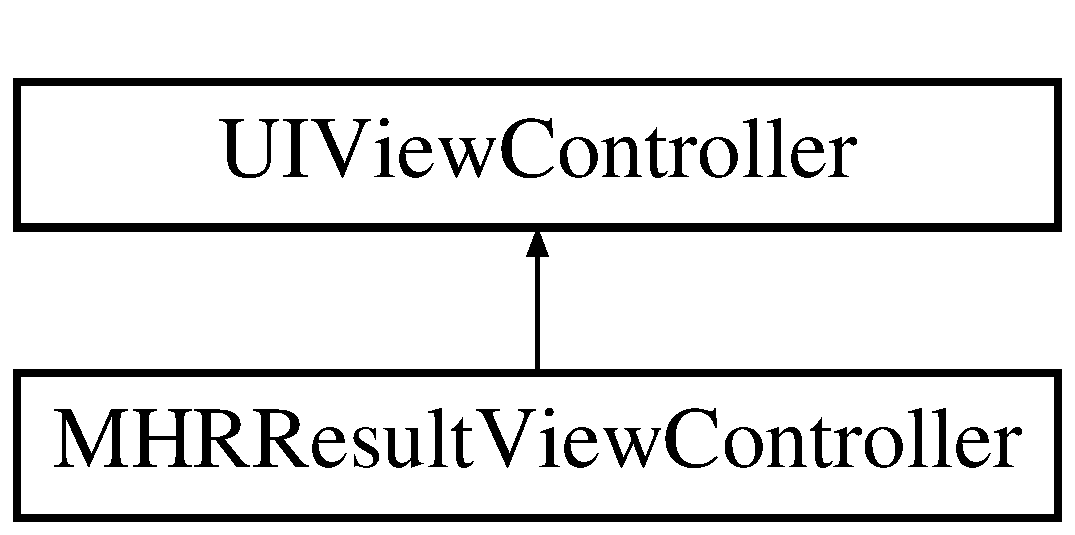
\includegraphics[height=2.000000cm]{interface_m_h_r_result_view_controller}
\end{center}
\end{figure}
\subsection*{Properties}
\begin{DoxyCompactItemize}
\item 
double \hyperlink{interface_m_h_r_result_view_controller_ad2cc92ee5ee811f8df6b04883f090096}{autocorr\+Result}
\item 
double \hyperlink{interface_m_h_r_result_view_controller_ae0daab10c086e438477f71f59fa0de37}{pda\+Result}
\end{DoxyCompactItemize}


\subsection{Detailed Description}


Definition at line 13 of file M\+H\+R\+Result\+View\+Controller.\+hpp.



\subsection{Property Documentation}
\hypertarget{interface_m_h_r_result_view_controller_ad2cc92ee5ee811f8df6b04883f090096}{\index{M\+H\+R\+Result\+View\+Controller@{M\+H\+R\+Result\+View\+Controller}!autocorr\+Result@{autocorr\+Result}}
\index{autocorr\+Result@{autocorr\+Result}!M\+H\+R\+Result\+View\+Controller@{M\+H\+R\+Result\+View\+Controller}}
\subsubsection[{autocorr\+Result}]{\setlength{\rightskip}{0pt plus 5cm}-\/ (double) autocorr\+Result\hspace{0.3cm}{\ttfamily [read]}, {\ttfamily [write]}, {\ttfamily [nonatomic]}, {\ttfamily [assign]}}}\label{interface_m_h_r_result_view_controller_ad2cc92ee5ee811f8df6b04883f090096}


Definition at line 15 of file M\+H\+R\+Result\+View\+Controller.\+hpp.

\hypertarget{interface_m_h_r_result_view_controller_ae0daab10c086e438477f71f59fa0de37}{\index{M\+H\+R\+Result\+View\+Controller@{M\+H\+R\+Result\+View\+Controller}!pda\+Result@{pda\+Result}}
\index{pda\+Result@{pda\+Result}!M\+H\+R\+Result\+View\+Controller@{M\+H\+R\+Result\+View\+Controller}}
\subsubsection[{pda\+Result}]{\setlength{\rightskip}{0pt plus 5cm}-\/ (double) pda\+Result\hspace{0.3cm}{\ttfamily [read]}, {\ttfamily [write]}, {\ttfamily [nonatomic]}, {\ttfamily [assign]}}}\label{interface_m_h_r_result_view_controller_ae0daab10c086e438477f71f59fa0de37}


Definition at line 16 of file M\+H\+R\+Result\+View\+Controller.\+hpp.



The documentation for this class was generated from the following file\+:\begin{DoxyCompactItemize}
\item 
Result\+View/\hyperlink{_m_h_r_result_view_controller_8hpp}{M\+H\+R\+Result\+View\+Controller.\+hpp}\end{DoxyCompactItemize}

\hypertarget{category_m_h_r_result_view_controller_07_08}{\section{M\+H\+R\+Result\+View\+Controller() Category Reference}
\label{category_m_h_r_result_view_controller_07_08}\index{M\+H\+R\+Result\+View\+Controller()@{M\+H\+R\+Result\+View\+Controller()}}
}
\subsection*{Properties}
\begin{DoxyCompactItemize}
\item 
I\+B\+Outlet U\+I\+Label $\ast$ \hyperlink{category_m_h_r_result_view_controller_07_08_a47e15cc9dd4edba89fabe5631de70baa}{autocorr\+Label}
\item 
I\+B\+Outlet U\+I\+Label $\ast$ \hyperlink{category_m_h_r_result_view_controller_07_08_a4d91971b1a4e42c64a1c0d2790b1fe53}{pda\+Label}
\end{DoxyCompactItemize}


\subsection{Detailed Description}


Definition at line 11 of file M\+H\+R\+Result\+View\+Controller.\+mm.



\subsection{Property Documentation}
\hypertarget{category_m_h_r_result_view_controller_07_08_a47e15cc9dd4edba89fabe5631de70baa}{\index{M\+H\+R\+Result\+View\+Controller()@{M\+H\+R\+Result\+View\+Controller()}!autocorr\+Label@{autocorr\+Label}}
\index{autocorr\+Label@{autocorr\+Label}!M\+H\+R\+Result\+View\+Controller()@{M\+H\+R\+Result\+View\+Controller()}}
\subsubsection[{autocorr\+Label}]{\setlength{\rightskip}{0pt plus 5cm}-\/ (I\+B\+Outlet U\+I\+Label$\ast$) autocorr\+Label\hspace{0.3cm}{\ttfamily [read]}, {\ttfamily [write]}, {\ttfamily [nonatomic]}, {\ttfamily [weak]}}}\label{category_m_h_r_result_view_controller_07_08_a47e15cc9dd4edba89fabe5631de70baa}


Definition at line 13 of file M\+H\+R\+Result\+View\+Controller.\+mm.

\hypertarget{category_m_h_r_result_view_controller_07_08_a4d91971b1a4e42c64a1c0d2790b1fe53}{\index{M\+H\+R\+Result\+View\+Controller()@{M\+H\+R\+Result\+View\+Controller()}!pda\+Label@{pda\+Label}}
\index{pda\+Label@{pda\+Label}!M\+H\+R\+Result\+View\+Controller()@{M\+H\+R\+Result\+View\+Controller()}}
\subsubsection[{pda\+Label}]{\setlength{\rightskip}{0pt plus 5cm}-\/ (I\+B\+Outlet U\+I\+Label$\ast$) pda\+Label\hspace{0.3cm}{\ttfamily [read]}, {\ttfamily [write]}, {\ttfamily [nonatomic]}, {\ttfamily [weak]}}}\label{category_m_h_r_result_view_controller_07_08_a4d91971b1a4e42c64a1c0d2790b1fe53}


Definition at line 14 of file M\+H\+R\+Result\+View\+Controller.\+mm.



The documentation for this category was generated from the following file\+:\begin{DoxyCompactItemize}
\item 
Misfit\+Heart\+Rate/\+Result\+View/\hyperlink{_m_h_r_result_view_controller_8mm}{M\+H\+R\+Result\+View\+Controller.\+mm}\end{DoxyCompactItemize}

\hypertarget{interface_m_h_r_settings_view_controller}{\section{M\+H\+R\+Settings\+View\+Controller Class Reference}
\label{interface_m_h_r_settings_view_controller}\index{M\+H\+R\+Settings\+View\+Controller@{M\+H\+R\+Settings\+View\+Controller}}
}


{\ttfamily \#import $<$M\+H\+R\+Settings\+View\+Controller.\+h$>$}

Inheritance diagram for M\+H\+R\+Settings\+View\+Controller\+:\begin{figure}[H]
\begin{center}
\leavevmode
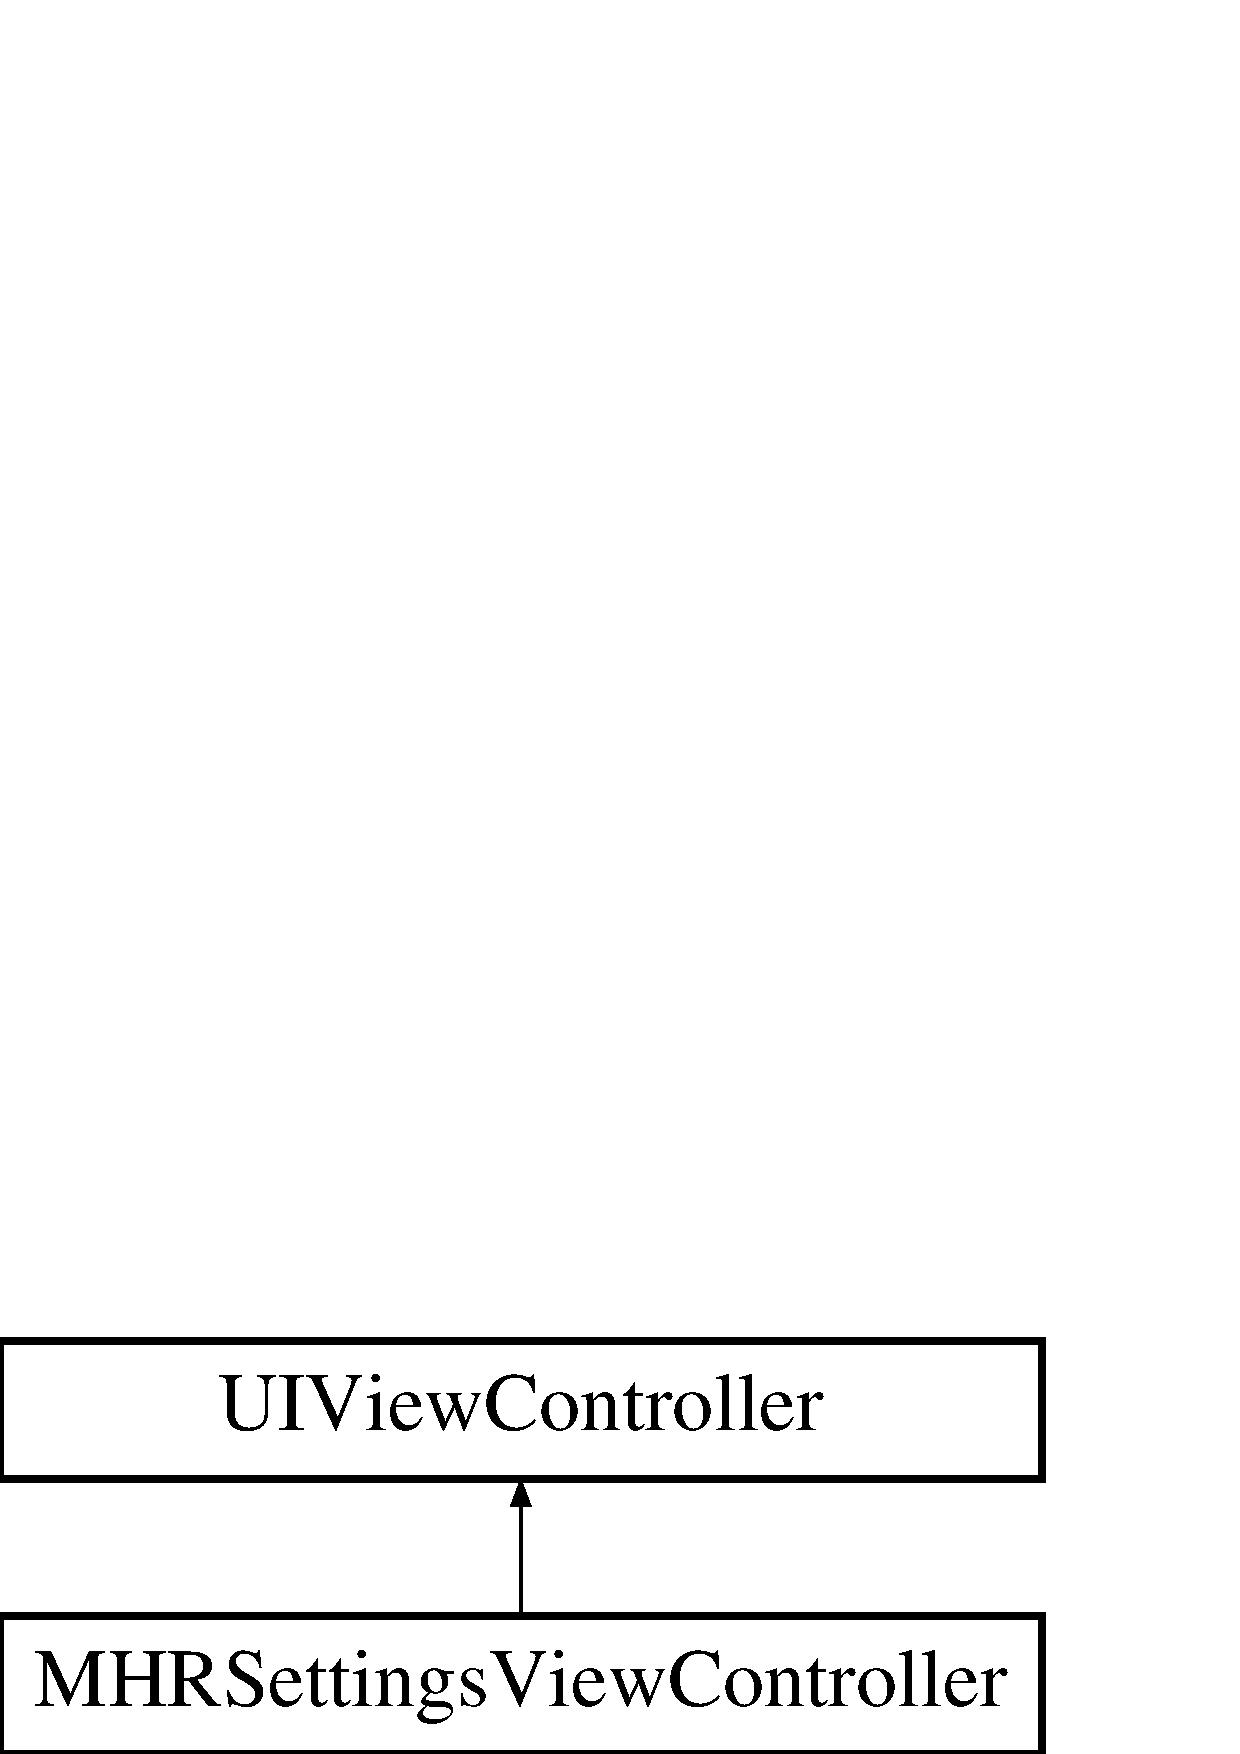
\includegraphics[height=2.000000cm]{interface_m_h_r_settings_view_controller}
\end{center}
\end{figure}
\subsection*{Protected Attributes}
\begin{DoxyCompactItemize}
\item 
id$<$ \hyperlink{protocol_m_h_r_settings_view_delegate-p}{M\+H\+R\+Settings\+View\+Delegate} $>$ \hyperlink{interface_m_h_r_settings_view_controller_a6fa685e4f9358a047d6f1cfd77f7ac0f}{\+\_\+delegate}
\end{DoxyCompactItemize}
\subsection*{Properties}
\begin{DoxyCompactItemize}
\item 
id \hyperlink{interface_m_h_r_settings_view_controller_a44380e171f6d773f58dc158ff58d47aa}{delegate}
\item 
B\+O\+O\+L \hyperlink{interface_m_h_r_settings_view_controller_abb8745a6f5f7529e69628d8f5f4f068e}{debug\+Mode\+On}
\item 
B\+O\+O\+L \hyperlink{interface_m_h_r_settings_view_controller_add55937fcb10a424e5f651d372b4b6a9}{three\+Chan\+Mode\+On}
\end{DoxyCompactItemize}


\subsection{Detailed Description}


Definition at line 20 of file M\+H\+R\+Settings\+View\+Controller.\+h.



\subsection{Member Data Documentation}
\hypertarget{interface_m_h_r_settings_view_controller_a6fa685e4f9358a047d6f1cfd77f7ac0f}{\index{M\+H\+R\+Settings\+View\+Controller@{M\+H\+R\+Settings\+View\+Controller}!\+\_\+delegate@{\+\_\+delegate}}
\index{\+\_\+delegate@{\+\_\+delegate}!M\+H\+R\+Settings\+View\+Controller@{M\+H\+R\+Settings\+View\+Controller}}
\subsubsection[{\+\_\+delegate}]{\setlength{\rightskip}{0pt plus 5cm}-\/ (id$<${\bf M\+H\+R\+Settings\+View\+Delegate}$>$) \+\_\+delegate\hspace{0.3cm}{\ttfamily [protected]}}}\label{interface_m_h_r_settings_view_controller_a6fa685e4f9358a047d6f1cfd77f7ac0f}


Definition at line 22 of file M\+H\+R\+Settings\+View\+Controller.\+h.



\subsection{Property Documentation}
\hypertarget{interface_m_h_r_settings_view_controller_abb8745a6f5f7529e69628d8f5f4f068e}{\index{M\+H\+R\+Settings\+View\+Controller@{M\+H\+R\+Settings\+View\+Controller}!debug\+Mode\+On@{debug\+Mode\+On}}
\index{debug\+Mode\+On@{debug\+Mode\+On}!M\+H\+R\+Settings\+View\+Controller@{M\+H\+R\+Settings\+View\+Controller}}
\subsubsection[{debug\+Mode\+On}]{\setlength{\rightskip}{0pt plus 5cm}-\/ (B\+O\+O\+L) debug\+Mode\+On\hspace{0.3cm}{\ttfamily [read]}, {\ttfamily [write]}, {\ttfamily [nonatomic]}, {\ttfamily [assign]}}}\label{interface_m_h_r_settings_view_controller_abb8745a6f5f7529e69628d8f5f4f068e}


Definition at line 27 of file M\+H\+R\+Settings\+View\+Controller.\+h.

\hypertarget{interface_m_h_r_settings_view_controller_a44380e171f6d773f58dc158ff58d47aa}{\index{M\+H\+R\+Settings\+View\+Controller@{M\+H\+R\+Settings\+View\+Controller}!delegate@{delegate}}
\index{delegate@{delegate}!M\+H\+R\+Settings\+View\+Controller@{M\+H\+R\+Settings\+View\+Controller}}
\subsubsection[{delegate}]{\setlength{\rightskip}{0pt plus 5cm}-\/ (id) delegate\hspace{0.3cm}{\ttfamily [read]}, {\ttfamily [write]}, {\ttfamily [nonatomic]}, {\ttfamily [strong]}}}\label{interface_m_h_r_settings_view_controller_a44380e171f6d773f58dc158ff58d47aa}


Definition at line 25 of file M\+H\+R\+Settings\+View\+Controller.\+h.

\hypertarget{interface_m_h_r_settings_view_controller_add55937fcb10a424e5f651d372b4b6a9}{\index{M\+H\+R\+Settings\+View\+Controller@{M\+H\+R\+Settings\+View\+Controller}!three\+Chan\+Mode\+On@{three\+Chan\+Mode\+On}}
\index{three\+Chan\+Mode\+On@{three\+Chan\+Mode\+On}!M\+H\+R\+Settings\+View\+Controller@{M\+H\+R\+Settings\+View\+Controller}}
\subsubsection[{three\+Chan\+Mode\+On}]{\setlength{\rightskip}{0pt plus 5cm}-\/ (B\+O\+O\+L) three\+Chan\+Mode\+On\hspace{0.3cm}{\ttfamily [read]}, {\ttfamily [write]}, {\ttfamily [nonatomic]}, {\ttfamily [assign]}}}\label{interface_m_h_r_settings_view_controller_add55937fcb10a424e5f651d372b4b6a9}


Definition at line 28 of file M\+H\+R\+Settings\+View\+Controller.\+h.



The documentation for this class was generated from the following file\+:\begin{DoxyCompactItemize}
\item 
Settings\+View/\hyperlink{_m_h_r_settings_view_controller_8h}{M\+H\+R\+Settings\+View\+Controller.\+h}\end{DoxyCompactItemize}

\hypertarget{category_m_h_r_settings_view_controller_07_08}{\section{M\+H\+R\+Settings\+View\+Controller() Category Reference}
\label{category_m_h_r_settings_view_controller_07_08}\index{M\+H\+R\+Settings\+View\+Controller()@{M\+H\+R\+Settings\+View\+Controller()}}
}
\subsection*{Properties}
\begin{DoxyCompactItemize}
\item 
I\+B\+Outlet U\+I\+Switch $\ast$ \hyperlink{category_m_h_r_settings_view_controller_07_08_a1aa168471752fac727fa69e4be17b438}{debug\+Mode\+Switch}
\item 
I\+B\+Outlet U\+I\+Switch $\ast$ \hyperlink{category_m_h_r_settings_view_controller_07_08_a1895b1abc4ef23d82293f905fbd27468}{three\+Chan\+Mode\+Switch}
\end{DoxyCompactItemize}


\subsection{Detailed Description}


Definition at line 11 of file M\+H\+R\+Settings\+View\+Controller.\+m.



\subsection{Property Documentation}
\hypertarget{category_m_h_r_settings_view_controller_07_08_a1aa168471752fac727fa69e4be17b438}{\index{M\+H\+R\+Settings\+View\+Controller()@{M\+H\+R\+Settings\+View\+Controller()}!debug\+Mode\+Switch@{debug\+Mode\+Switch}}
\index{debug\+Mode\+Switch@{debug\+Mode\+Switch}!M\+H\+R\+Settings\+View\+Controller()@{M\+H\+R\+Settings\+View\+Controller()}}
\subsubsection[{debug\+Mode\+Switch}]{\setlength{\rightskip}{0pt plus 5cm}-\/ (I\+B\+Outlet U\+I\+Switch$\ast$) debug\+Mode\+Switch\hspace{0.3cm}{\ttfamily [read]}, {\ttfamily [write]}, {\ttfamily [nonatomic]}, {\ttfamily [weak]}}}\label{category_m_h_r_settings_view_controller_07_08_a1aa168471752fac727fa69e4be17b438}


Definition at line 13 of file M\+H\+R\+Settings\+View\+Controller.\+m.

\hypertarget{category_m_h_r_settings_view_controller_07_08_a1895b1abc4ef23d82293f905fbd27468}{\index{M\+H\+R\+Settings\+View\+Controller()@{M\+H\+R\+Settings\+View\+Controller()}!three\+Chan\+Mode\+Switch@{three\+Chan\+Mode\+Switch}}
\index{three\+Chan\+Mode\+Switch@{three\+Chan\+Mode\+Switch}!M\+H\+R\+Settings\+View\+Controller()@{M\+H\+R\+Settings\+View\+Controller()}}
\subsubsection[{three\+Chan\+Mode\+Switch}]{\setlength{\rightskip}{0pt plus 5cm}-\/ (I\+B\+Outlet U\+I\+Switch$\ast$) three\+Chan\+Mode\+Switch\hspace{0.3cm}{\ttfamily [read]}, {\ttfamily [write]}, {\ttfamily [nonatomic]}, {\ttfamily [weak]}}}\label{category_m_h_r_settings_view_controller_07_08_a1895b1abc4ef23d82293f905fbd27468}


Definition at line 14 of file M\+H\+R\+Settings\+View\+Controller.\+m.



The documentation for this category was generated from the following file\+:\begin{DoxyCompactItemize}
\item 
Misfit\+Heart\+Rate/\+Settings\+View/\hyperlink{_m_h_r_settings_view_controller_8m}{M\+H\+R\+Settings\+View\+Controller.\+m}\end{DoxyCompactItemize}

\hypertarget{protocol_m_h_r_settings_view_delegate-p}{\section{$<$M\+H\+R\+Settings\+View\+Delegate$>$ Protocol Reference}
\label{protocol_m_h_r_settings_view_delegate-p}\index{$<$\+M\+H\+R\+Settings\+View\+Delegate$>$@{$<$\+M\+H\+R\+Settings\+View\+Delegate$>$}}
}


{\ttfamily \#import $<$M\+H\+R\+Settings\+View\+Controller.\+h$>$}

Inheritance diagram for $<$M\+H\+R\+Settings\+View\+Delegate$>$\+:\begin{figure}[H]
\begin{center}
\leavevmode
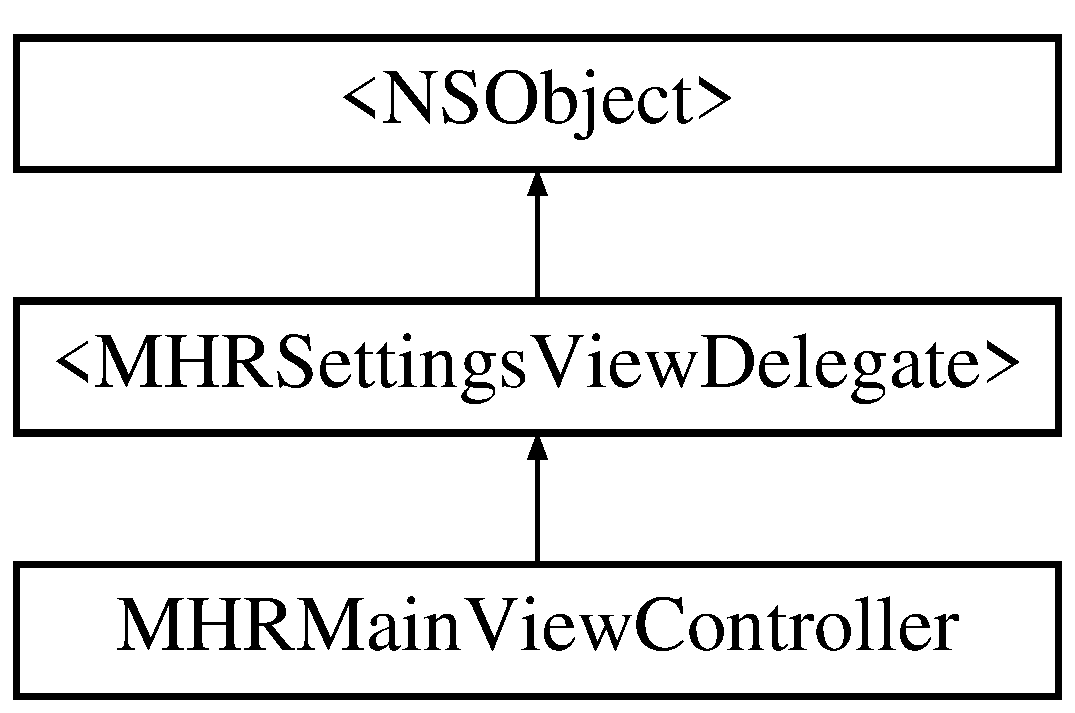
\includegraphics[height=3.000000cm]{protocol_m_h_r_settings_view_delegate-p}
\end{center}
\end{figure}
\subsection*{Instance Methods}
\begin{DoxyCompactItemize}
\item 
(void) -\/ \hyperlink{protocol_m_h_r_settings_view_delegate-p_a1d7367b2d59c2dce76e953607bdc032e}{debug\+Mode\+Changed\+:}
\item 
(void) -\/ \hyperlink{protocol_m_h_r_settings_view_delegate-p_ade012e6adf8df6a09d7a51909815f360}{three\+Chan\+Mode\+Changed\+:}
\end{DoxyCompactItemize}


\subsection{Detailed Description}


Definition at line 11 of file M\+H\+R\+Settings\+View\+Controller.\+h.



\subsection{Method Documentation}
\hypertarget{protocol_m_h_r_settings_view_delegate-p_a1d7367b2d59c2dce76e953607bdc032e}{\index{M\+H\+R\+Settings\+View\+Delegate-\/p@{M\+H\+R\+Settings\+View\+Delegate-\/p}!debug\+Mode\+Changed\+:@{debug\+Mode\+Changed\+:}}
\index{debug\+Mode\+Changed\+:@{debug\+Mode\+Changed\+:}!M\+H\+R\+Settings\+View\+Delegate-\/p@{M\+H\+R\+Settings\+View\+Delegate-\/p}}
\subsubsection[{debug\+Mode\+Changed\+:}]{\setlength{\rightskip}{0pt plus 5cm}-\/ (void) debug\+Mode\+Changed\+: 
\begin{DoxyParamCaption}
\item[{(B\+O\+O\+L)}]{mode}
\end{DoxyParamCaption}
\hspace{0.3cm}{\ttfamily [required]}}}\label{protocol_m_h_r_settings_view_delegate-p_a1d7367b2d59c2dce76e953607bdc032e}
\hypertarget{protocol_m_h_r_settings_view_delegate-p_ade012e6adf8df6a09d7a51909815f360}{\index{M\+H\+R\+Settings\+View\+Delegate-\/p@{M\+H\+R\+Settings\+View\+Delegate-\/p}!three\+Chan\+Mode\+Changed\+:@{three\+Chan\+Mode\+Changed\+:}}
\index{three\+Chan\+Mode\+Changed\+:@{three\+Chan\+Mode\+Changed\+:}!M\+H\+R\+Settings\+View\+Delegate-\/p@{M\+H\+R\+Settings\+View\+Delegate-\/p}}
\subsubsection[{three\+Chan\+Mode\+Changed\+:}]{\setlength{\rightskip}{0pt plus 5cm}-\/ (void) three\+Chan\+Mode\+Changed\+: 
\begin{DoxyParamCaption}
\item[{(B\+O\+O\+L)}]{mode}
\end{DoxyParamCaption}
\hspace{0.3cm}{\ttfamily [required]}}}\label{protocol_m_h_r_settings_view_delegate-p_ade012e6adf8df6a09d7a51909815f360}


The documentation for this protocol was generated from the following file\+:\begin{DoxyCompactItemize}
\item 
Misfit\+Heart\+Rate/\+Settings\+View/\hyperlink{_m_h_r_settings_view_controller_8h}{M\+H\+R\+Settings\+View\+Controller.\+h}\end{DoxyCompactItemize}

\hypertarget{interface_m_h_r_utilities}{\section{M\+H\+R\+Utilities Class Reference}
\label{interface_m_h_r_utilities}\index{M\+H\+R\+Utilities@{M\+H\+R\+Utilities}}
}


{\ttfamily \#import $<$M\+H\+R\+Utilities.\+h$>$}

Inheritance diagram for M\+H\+R\+Utilities\+:\begin{figure}[H]
\begin{center}
\leavevmode
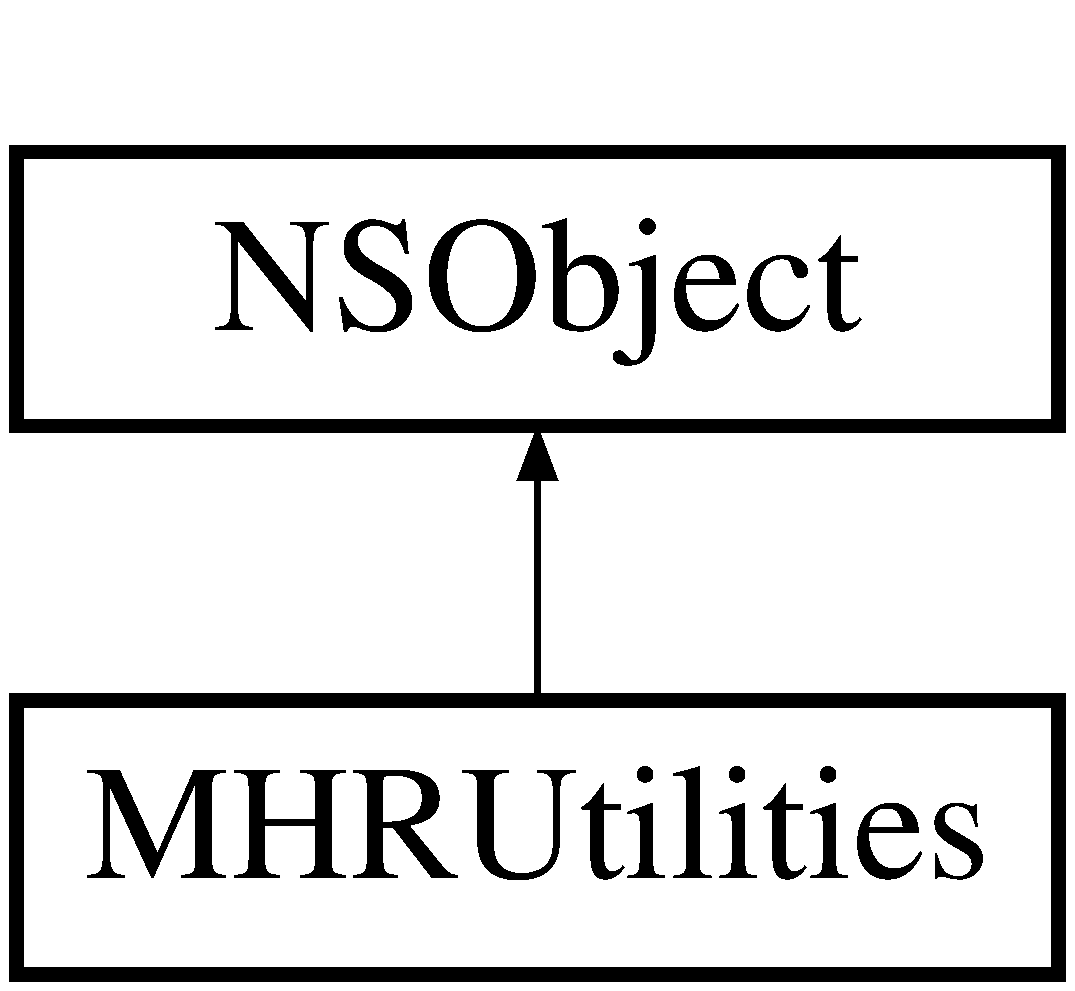
\includegraphics[height=2.000000cm]{interface_m_h_r_utilities}
\end{center}
\end{figure}
\subsection*{Instance Methods}
\begin{DoxyCompactItemize}
\item 
(U\+I\+Color $\ast$) -\/ \hyperlink{interface_m_h_r_utilities_a92885094add75d90dfb00faaf36d423e}{M\+F\+U\+I\+Color\+Make\+From\+R\+G\+B\+Array}
\item 
(U\+I\+Color $\ast$) -\/ \hyperlink{interface_m_h_r_utilities_a824edf59b4a4e127db0f4248c4d4bfd6}{M\+F\+U\+I\+Color\+Make\+From\+R\+G\+B\+A\+Array}
\end{DoxyCompactItemize}
\subsection*{Class Methods}
\begin{DoxyCompactItemize}
\item 
(N\+S\+String $\ast$) + \hyperlink{interface_m_h_r_utilities_a1f7c42bb731cae8fb90d106014b00df9}{report\+\_\+memory}
\item 
(void) + \hyperlink{interface_m_h_r_utilities_a85f3406abe6ae8911d4a8349996e1d6c}{create\+Directory\+:}
\item 
(void) + \hyperlink{interface_m_h_r_utilities_a4c2719ba1e46c5491a9868ab93dc8cfe}{set\+Torch\+Mode\+On\+:}
\item 
(C\+A\+Layer $\ast$) + \hyperlink{interface_m_h_r_utilities_aced58e360114134fcc1982a6862fc523}{new\+Rectangle\+Layer\+:p\+List\+Key\+:}
\end{DoxyCompactItemize}


\subsection{Detailed Description}


Definition at line 16 of file M\+H\+R\+Utilities.\+h.



\subsection{Method Documentation}
\hypertarget{interface_m_h_r_utilities_a85f3406abe6ae8911d4a8349996e1d6c}{\index{M\+H\+R\+Utilities@{M\+H\+R\+Utilities}!create\+Directory\+:@{create\+Directory\+:}}
\index{create\+Directory\+:@{create\+Directory\+:}!M\+H\+R\+Utilities@{M\+H\+R\+Utilities}}
\subsubsection[{create\+Directory\+:}]{\setlength{\rightskip}{0pt plus 5cm}+ (void) create\+Directory\+: 
\begin{DoxyParamCaption}
\item[{(N\+S\+String $\ast$)}]{directory\+Path}
\end{DoxyParamCaption}
}}\label{interface_m_h_r_utilities_a85f3406abe6ae8911d4a8349996e1d6c}


Definition at line 37 of file M\+H\+R\+Utilities.\+m.

\hypertarget{interface_m_h_r_utilities_a824edf59b4a4e127db0f4248c4d4bfd6}{\index{M\+H\+R\+Utilities@{M\+H\+R\+Utilities}!M\+F\+U\+I\+Color\+Make\+From\+R\+G\+B\+A\+Array@{M\+F\+U\+I\+Color\+Make\+From\+R\+G\+B\+A\+Array}}
\index{M\+F\+U\+I\+Color\+Make\+From\+R\+G\+B\+A\+Array@{M\+F\+U\+I\+Color\+Make\+From\+R\+G\+B\+A\+Array}!M\+H\+R\+Utilities@{M\+H\+R\+Utilities}}
\subsubsection[{M\+F\+U\+I\+Color\+Make\+From\+R\+G\+B\+A\+Array}]{\setlength{\rightskip}{0pt plus 5cm}-\/ (U\+I\+Color $\ast$) M\+F\+U\+I\+Color\+Make\+From\+R\+G\+B\+A\+Array 
\begin{DoxyParamCaption}
\item[{(N\+S\+Array $\ast$)}]{rgba\+Array}
\end{DoxyParamCaption}
}}\label{interface_m_h_r_utilities_a824edf59b4a4e127db0f4248c4d4bfd6}


Definition at line 79 of file M\+H\+R\+Utilities.\+m.

\hypertarget{interface_m_h_r_utilities_a92885094add75d90dfb00faaf36d423e}{\index{M\+H\+R\+Utilities@{M\+H\+R\+Utilities}!M\+F\+U\+I\+Color\+Make\+From\+R\+G\+B\+Array@{M\+F\+U\+I\+Color\+Make\+From\+R\+G\+B\+Array}}
\index{M\+F\+U\+I\+Color\+Make\+From\+R\+G\+B\+Array@{M\+F\+U\+I\+Color\+Make\+From\+R\+G\+B\+Array}!M\+H\+R\+Utilities@{M\+H\+R\+Utilities}}
\subsubsection[{M\+F\+U\+I\+Color\+Make\+From\+R\+G\+B\+Array}]{\setlength{\rightskip}{0pt plus 5cm}-\/ (U\+I\+Color $\ast$) M\+F\+U\+I\+Color\+Make\+From\+R\+G\+B\+Array 
\begin{DoxyParamCaption}
\item[{(N\+S\+Array $\ast$)}]{rgb\+Array}
\end{DoxyParamCaption}
}}\label{interface_m_h_r_utilities_a92885094add75d90dfb00faaf36d423e}


Definition at line 70 of file M\+H\+R\+Utilities.\+m.

\hypertarget{interface_m_h_r_utilities_aced58e360114134fcc1982a6862fc523}{\index{M\+H\+R\+Utilities@{M\+H\+R\+Utilities}!new\+Rectangle\+Layer\+:p\+List\+Key\+:@{new\+Rectangle\+Layer\+:p\+List\+Key\+:}}
\index{new\+Rectangle\+Layer\+:p\+List\+Key\+:@{new\+Rectangle\+Layer\+:p\+List\+Key\+:}!M\+H\+R\+Utilities@{M\+H\+R\+Utilities}}
\subsubsection[{new\+Rectangle\+Layer\+:p\+List\+Key\+:}]{\setlength{\rightskip}{0pt plus 5cm}+ (C\+A\+Layer $\ast$) new\+Rectangle\+Layer\+: 
\begin{DoxyParamCaption}
\item[{(C\+G\+Rect)}]{frame}
\item[{pListKey:(N\+S\+String $\ast$)}]{p\+List\+Key}
\end{DoxyParamCaption}
}}\label{interface_m_h_r_utilities_aced58e360114134fcc1982a6862fc523}


Definition at line 89 of file M\+H\+R\+Utilities.\+m.

\hypertarget{interface_m_h_r_utilities_a1f7c42bb731cae8fb90d106014b00df9}{\index{M\+H\+R\+Utilities@{M\+H\+R\+Utilities}!report\+\_\+memory@{report\+\_\+memory}}
\index{report\+\_\+memory@{report\+\_\+memory}!M\+H\+R\+Utilities@{M\+H\+R\+Utilities}}
\subsubsection[{report\+\_\+memory}]{\setlength{\rightskip}{0pt plus 5cm}+ (N\+S\+String $\ast$) report\+\_\+memory 
\begin{DoxyParamCaption}
{}
\end{DoxyParamCaption}
}}\label{interface_m_h_r_utilities_a1f7c42bb731cae8fb90d106014b00df9}


Definition at line 16 of file M\+H\+R\+Utilities.\+m.

\hypertarget{interface_m_h_r_utilities_a4c2719ba1e46c5491a9868ab93dc8cfe}{\index{M\+H\+R\+Utilities@{M\+H\+R\+Utilities}!set\+Torch\+Mode\+On\+:@{set\+Torch\+Mode\+On\+:}}
\index{set\+Torch\+Mode\+On\+:@{set\+Torch\+Mode\+On\+:}!M\+H\+R\+Utilities@{M\+H\+R\+Utilities}}
\subsubsection[{set\+Torch\+Mode\+On\+:}]{\setlength{\rightskip}{0pt plus 5cm}+ (void) set\+Torch\+Mode\+On\+: 
\begin{DoxyParamCaption}
\item[{(B\+O\+O\+L)}]{is\+On}
\end{DoxyParamCaption}
}}\label{interface_m_h_r_utilities_a4c2719ba1e46c5491a9868ab93dc8cfe}


Definition at line 50 of file M\+H\+R\+Utilities.\+m.



The documentation for this class was generated from the following files\+:\begin{DoxyCompactItemize}
\item 
Misfit\+Heart\+Rate/\+Utilities/\hyperlink{_m_h_r_utilities_8h}{M\+H\+R\+Utilities.\+h}\item 
Misfit\+Heart\+Rate/\+Utilities/\hyperlink{_m_h_r_utilities_8m}{M\+H\+R\+Utilities.\+m}\end{DoxyCompactItemize}

\hypertarget{category_u_i_alert_view_07_block_08}{\section{U\+I\+Alert\+View(Block) Category Reference}
\label{category_u_i_alert_view_07_block_08}\index{U\+I\+Alert\+View(\+Block)@{U\+I\+Alert\+View(\+Block)}}
}


\subsection{Detailed Description}


Definition at line 18 of file U\+I\+Alert\+View+\+Block.\+m.



The documentation for this category was generated from the following file\+:\begin{DoxyCompactItemize}
\item 
Misfit\+Heart\+Rate/\+Utilities/\hyperlink{_u_i_alert_view_09_block_8m}{U\+I\+Alert\+View+\+Block.\+m}\end{DoxyCompactItemize}

\hypertarget{interface_u_i_image_c_v_mat_converter}{\section{U\+I\+Image\+C\+V\+Mat\+Converter Class Reference}
\label{interface_u_i_image_c_v_mat_converter}\index{U\+I\+Image\+C\+V\+Mat\+Converter@{U\+I\+Image\+C\+V\+Mat\+Converter}}
}


{\ttfamily \#import $<$U\+I\+Image\+C\+V\+Mat\+Converter.\+hpp$>$}

Inheritance diagram for U\+I\+Image\+C\+V\+Mat\+Converter\+:\begin{figure}[H]
\begin{center}
\leavevmode
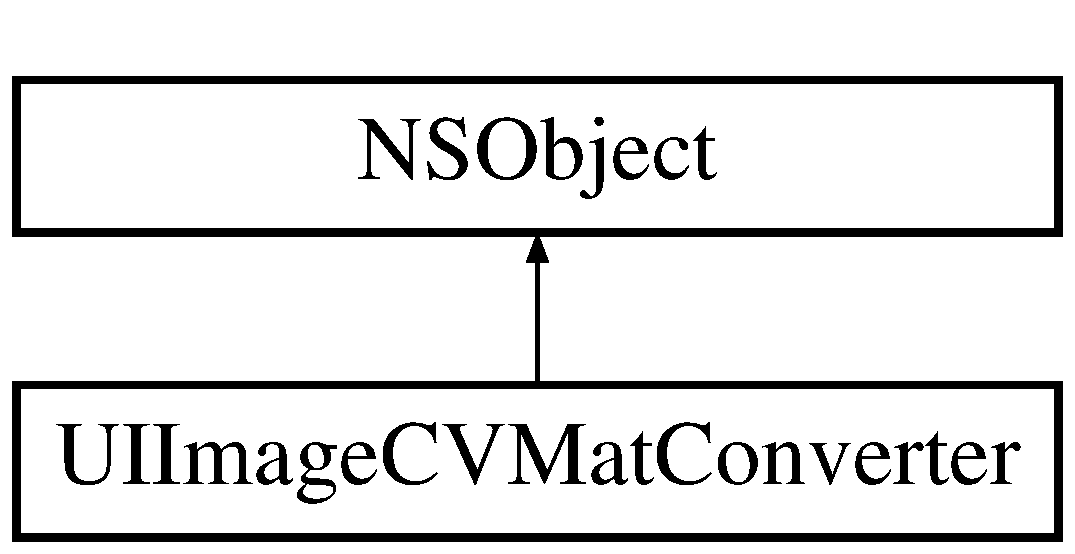
\includegraphics[height=2.000000cm]{interface_u_i_image_c_v_mat_converter}
\end{center}
\end{figure}
\subsection*{Class Methods}
\begin{DoxyCompactItemize}
\item 
(U\+I\+Image $\ast$) + \hyperlink{interface_u_i_image_c_v_mat_converter_ae96cde81129f965a43427053199cd92d}{U\+I\+Image\+From\+C\+V\+Mat\+:}
\item 
(U\+I\+Image $\ast$) + \hyperlink{interface_u_i_image_c_v_mat_converter_abd5e5c4c7280d04fffea79737b556507}{U\+I\+Image\+From\+C\+V\+Mat\+:with\+U\+I\+Image\+:}
\item 
(cv\+::\+Mat) + \hyperlink{interface_u_i_image_c_v_mat_converter_abeefe1d140e9bdd660b07d1dabce66f1}{cv\+Mat\+From\+U\+I\+Image\+:}
\item 
(cv\+::\+Mat) + \hyperlink{interface_u_i_image_c_v_mat_converter_adcff189c46b8a96188a10775f133138f}{cv\+Mat\+Gray\+From\+U\+I\+Image\+:}
\item 
(U\+I\+Image $\ast$) + \hyperlink{interface_u_i_image_c_v_mat_converter_a6f3591f2805f153289fae9fb8e50ca67}{scale\+And\+Rotate\+Image\+Front\+Camera\+:}
\item 
(U\+I\+Image $\ast$) + \hyperlink{interface_u_i_image_c_v_mat_converter_a92e5de957061495ab6c3f1cadfafa2f9}{scale\+And\+Rotate\+Image\+Back\+Camera\+:}
\end{DoxyCompactItemize}


\subsection{Detailed Description}


Definition at line 15 of file U\+I\+Image\+C\+V\+Mat\+Converter.\+hpp.



\subsection{Method Documentation}
\hypertarget{interface_u_i_image_c_v_mat_converter_abeefe1d140e9bdd660b07d1dabce66f1}{\index{U\+I\+Image\+C\+V\+Mat\+Converter@{U\+I\+Image\+C\+V\+Mat\+Converter}!cv\+Mat\+From\+U\+I\+Image\+:@{cv\+Mat\+From\+U\+I\+Image\+:}}
\index{cv\+Mat\+From\+U\+I\+Image\+:@{cv\+Mat\+From\+U\+I\+Image\+:}!U\+I\+Image\+C\+V\+Mat\+Converter@{U\+I\+Image\+C\+V\+Mat\+Converter}}
\subsubsection[{cv\+Mat\+From\+U\+I\+Image\+:}]{\setlength{\rightskip}{0pt plus 5cm}+ (Mat) U\+I\+Image\+C\+V\+Mat\+Converter\+: 
\begin{DoxyParamCaption}
\item[{(U\+I\+Image $\ast$)}]{image}
\end{DoxyParamCaption}
}}\label{interface_u_i_image_c_v_mat_converter_abeefe1d140e9bdd660b07d1dabce66f1}


Definition at line 84 of file U\+I\+Image\+C\+V\+Mat\+Converter.\+mm.

\hypertarget{interface_u_i_image_c_v_mat_converter_adcff189c46b8a96188a10775f133138f}{\index{U\+I\+Image\+C\+V\+Mat\+Converter@{U\+I\+Image\+C\+V\+Mat\+Converter}!cv\+Mat\+Gray\+From\+U\+I\+Image\+:@{cv\+Mat\+Gray\+From\+U\+I\+Image\+:}}
\index{cv\+Mat\+Gray\+From\+U\+I\+Image\+:@{cv\+Mat\+Gray\+From\+U\+I\+Image\+:}!U\+I\+Image\+C\+V\+Mat\+Converter@{U\+I\+Image\+C\+V\+Mat\+Converter}}
\subsubsection[{cv\+Mat\+Gray\+From\+U\+I\+Image\+:}]{\setlength{\rightskip}{0pt plus 5cm}+ (Mat) U\+I\+Image\+C\+V\+Mat\+Converter\+: 
\begin{DoxyParamCaption}
\item[{(U\+I\+Image $\ast$)}]{image}
\end{DoxyParamCaption}
}}\label{interface_u_i_image_c_v_mat_converter_adcff189c46b8a96188a10775f133138f}


Definition at line 109 of file U\+I\+Image\+C\+V\+Mat\+Converter.\+mm.

\hypertarget{interface_u_i_image_c_v_mat_converter_a92e5de957061495ab6c3f1cadfafa2f9}{\index{U\+I\+Image\+C\+V\+Mat\+Converter@{U\+I\+Image\+C\+V\+Mat\+Converter}!scale\+And\+Rotate\+Image\+Back\+Camera\+:@{scale\+And\+Rotate\+Image\+Back\+Camera\+:}}
\index{scale\+And\+Rotate\+Image\+Back\+Camera\+:@{scale\+And\+Rotate\+Image\+Back\+Camera\+:}!U\+I\+Image\+C\+V\+Mat\+Converter@{U\+I\+Image\+C\+V\+Mat\+Converter}}
\subsubsection[{scale\+And\+Rotate\+Image\+Back\+Camera\+:}]{\setlength{\rightskip}{0pt plus 5cm}+ (U\+I\+Image $\ast$) scale\+And\+Rotate\+Image\+Back\+Camera\+: 
\begin{DoxyParamCaption}
\item[{(U\+I\+Image $\ast$)}]{image}
\end{DoxyParamCaption}
}}\label{interface_u_i_image_c_v_mat_converter_a92e5de957061495ab6c3f1cadfafa2f9}


Definition at line 124 of file U\+I\+Image\+C\+V\+Mat\+Converter.\+mm.

\hypertarget{interface_u_i_image_c_v_mat_converter_a6f3591f2805f153289fae9fb8e50ca67}{\index{U\+I\+Image\+C\+V\+Mat\+Converter@{U\+I\+Image\+C\+V\+Mat\+Converter}!scale\+And\+Rotate\+Image\+Front\+Camera\+:@{scale\+And\+Rotate\+Image\+Front\+Camera\+:}}
\index{scale\+And\+Rotate\+Image\+Front\+Camera\+:@{scale\+And\+Rotate\+Image\+Front\+Camera\+:}!U\+I\+Image\+C\+V\+Mat\+Converter@{U\+I\+Image\+C\+V\+Mat\+Converter}}
\subsubsection[{scale\+And\+Rotate\+Image\+Front\+Camera\+:}]{\setlength{\rightskip}{0pt plus 5cm}+ (U\+I\+Image $\ast$) scale\+And\+Rotate\+Image\+Front\+Camera\+: 
\begin{DoxyParamCaption}
\item[{(U\+I\+Image $\ast$)}]{image}
\end{DoxyParamCaption}
}}\label{interface_u_i_image_c_v_mat_converter_a6f3591f2805f153289fae9fb8e50ca67}


Definition at line 216 of file U\+I\+Image\+C\+V\+Mat\+Converter.\+mm.

\hypertarget{interface_u_i_image_c_v_mat_converter_ae96cde81129f965a43427053199cd92d}{\index{U\+I\+Image\+C\+V\+Mat\+Converter@{U\+I\+Image\+C\+V\+Mat\+Converter}!U\+I\+Image\+From\+C\+V\+Mat\+:@{U\+I\+Image\+From\+C\+V\+Mat\+:}}
\index{U\+I\+Image\+From\+C\+V\+Mat\+:@{U\+I\+Image\+From\+C\+V\+Mat\+:}!U\+I\+Image\+C\+V\+Mat\+Converter@{U\+I\+Image\+C\+V\+Mat\+Converter}}
\subsubsection[{U\+I\+Image\+From\+C\+V\+Mat\+:}]{\setlength{\rightskip}{0pt plus 5cm}+ (U\+I\+Image $\ast$) U\+I\+Image\+From\+C\+V\+Mat\+: 
\begin{DoxyParamCaption}
\item[{(cv\+::\+Mat)}]{cv\+Mat}
\end{DoxyParamCaption}
}}\label{interface_u_i_image_c_v_mat_converter_ae96cde81129f965a43427053199cd92d}


Definition at line 48 of file U\+I\+Image\+C\+V\+Mat\+Converter.\+mm.

\hypertarget{interface_u_i_image_c_v_mat_converter_abd5e5c4c7280d04fffea79737b556507}{\index{U\+I\+Image\+C\+V\+Mat\+Converter@{U\+I\+Image\+C\+V\+Mat\+Converter}!U\+I\+Image\+From\+C\+V\+Mat\+:with\+U\+I\+Image\+:@{U\+I\+Image\+From\+C\+V\+Mat\+:with\+U\+I\+Image\+:}}
\index{U\+I\+Image\+From\+C\+V\+Mat\+:with\+U\+I\+Image\+:@{U\+I\+Image\+From\+C\+V\+Mat\+:with\+U\+I\+Image\+:}!U\+I\+Image\+C\+V\+Mat\+Converter@{U\+I\+Image\+C\+V\+Mat\+Converter}}
\subsubsection[{U\+I\+Image\+From\+C\+V\+Mat\+:with\+U\+I\+Image\+:}]{\setlength{\rightskip}{0pt plus 5cm}+ (U\+I\+Image $\ast$) {\bf U\+I\+Image\+From\+C\+V\+Mat\+:} 
\begin{DoxyParamCaption}
\item[{(cv\+::\+Mat)}]{cv\+Mat}
\item[{withUIImage:(U\+I\+Image$\ast$)}]{image}
\end{DoxyParamCaption}
}}\label{interface_u_i_image_c_v_mat_converter_abd5e5c4c7280d04fffea79737b556507}


Definition at line 16 of file U\+I\+Image\+C\+V\+Mat\+Converter.\+mm.



The documentation for this class was generated from the following files\+:\begin{DoxyCompactItemize}
\item 
Utilities/\hyperlink{_u_i_image_c_v_mat_converter_8hpp}{U\+I\+Image\+C\+V\+Mat\+Converter.\+hpp}\item 
Utilities/\hyperlink{_u_i_image_c_v_mat_converter_8mm}{U\+I\+Image\+C\+V\+Mat\+Converter.\+mm}\end{DoxyCompactItemize}

\hypertarget{category_u_i_view_07_position_08}{\section{U\+I\+View(Position) Category Reference}
\label{category_u_i_view_07_position_08}\index{U\+I\+View(\+Position)@{U\+I\+View(\+Position)}}
}


{\ttfamily \#import $<$U\+I\+View+\+Position.\+h$>$}

\subsection*{Instance Methods}
\begin{DoxyCompactItemize}
\item 
(void) -\/ \hyperlink{category_u_i_view_07_position_08_a4ab53ef69f304fba4732aeb9256b5ee0}{add\+Centered\+Subview\+:}
\item 
(void) -\/ \hyperlink{category_u_i_view_07_position_08_afaae9a5b1741fa3eb2ae7c57cf4687d8}{move\+To\+Center\+Of\+Superview}
\item 
(void) -\/ \hyperlink{category_u_i_view_07_position_08_a3ede327c32904e3e1e9e5c90b6cd8071}{center\+Vertically\+In\+Superview}
\item 
(void) -\/ \hyperlink{category_u_i_view_07_position_08_a50aabdd38d9ff4e017bc0238e2346ae2}{center\+Horizontally\+In\+Superview}
\item 
(void) -\/ \hyperlink{category_u_i_view_07_position_08_aee174d95a8088008dd006205fad44d17}{set\+Frame\+X\+Plus\+:y\+Plus\+:width\+Plus\+:height\+Plus\+:}
\item 
(void) -\/ \hyperlink{category_u_i_view_07_position_08_a3f7385a31ead16eb46e759a413aa9f19}{adjust\+Frame\+Formi\+O\+S6\+Toi\+O\+S7\+:}
\item 
(void) -\/ \hyperlink{category_u_i_view_07_position_08_a26680d798543876e3d295c69ecf7f35c}{adjust\+Frame\+Formi\+O\+S7\+Toi\+O\+S6\+:}
\end{DoxyCompactItemize}
\subsection*{Properties}
\begin{DoxyCompactItemize}
\item 
C\+G\+Point \hyperlink{category_u_i_view_07_position_08_af1d70399207fb8befa7e0f287bf23368}{frame\+Origin}
\item 
C\+G\+Size \hyperlink{category_u_i_view_07_position_08_afa9efa5679d7caac0a6a03f6e71342de}{frame\+Size}
\item 
C\+G\+Float \hyperlink{category_u_i_view_07_position_08_a16476712cc236d743510b2f39363396d}{frame\+X}
\item 
C\+G\+Float \hyperlink{category_u_i_view_07_position_08_a60a2692ff93131e7bbba22ecf3726f55}{frame\+Y}
\item 
C\+G\+Float \hyperlink{category_u_i_view_07_position_08_a203a633f161baa33534255efff338ec3}{frame\+Right}
\item 
C\+G\+Float \hyperlink{category_u_i_view_07_position_08_a6a730310961d877923cbe081dc3e5b39}{frame\+Bottom}
\item 
C\+G\+Float \hyperlink{category_u_i_view_07_position_08_aff1bcfa93fa19e1ed68022c263452a3b}{frame\+Width}
\item 
C\+G\+Float \hyperlink{category_u_i_view_07_position_08_a96659e2eec8d359d96a460582247f4c8}{frame\+Height}
\end{DoxyCompactItemize}


\subsection{Detailed Description}


Definition at line 22 of file U\+I\+View+\+Position.\+h.



\subsection{Method Documentation}
\hypertarget{category_u_i_view_07_position_08_a4ab53ef69f304fba4732aeb9256b5ee0}{\index{U\+I\+View(\+Position)@{U\+I\+View(\+Position)}!add\+Centered\+Subview\+:@{add\+Centered\+Subview\+:}}
\index{add\+Centered\+Subview\+:@{add\+Centered\+Subview\+:}!U\+I\+View(\+Position)@{U\+I\+View(\+Position)}}
\subsubsection[{add\+Centered\+Subview\+:}]{\setlength{\rightskip}{0pt plus 5cm}-\/ (void) add\+Centered\+Subview\+: 
\begin{DoxyParamCaption}
\item[{(U\+I\+View $\ast$)}]{subview}
\end{DoxyParamCaption}
}}\label{category_u_i_view_07_position_08_a4ab53ef69f304fba4732aeb9256b5ee0}


Definition at line 84 of file U\+I\+View+\+Position.\+m.

\hypertarget{category_u_i_view_07_position_08_a3f7385a31ead16eb46e759a413aa9f19}{\index{U\+I\+View(\+Position)@{U\+I\+View(\+Position)}!adjust\+Frame\+Formi\+O\+S6\+Toi\+O\+S7\+:@{adjust\+Frame\+Formi\+O\+S6\+Toi\+O\+S7\+:}}
\index{adjust\+Frame\+Formi\+O\+S6\+Toi\+O\+S7\+:@{adjust\+Frame\+Formi\+O\+S6\+Toi\+O\+S7\+:}!U\+I\+View(\+Position)@{U\+I\+View(\+Position)}}
\subsubsection[{adjust\+Frame\+Formi\+O\+S6\+Toi\+O\+S7\+:}]{\setlength{\rightskip}{0pt plus 5cm}-\/ (void) adjust\+Frame\+Formi\+O\+S6\+Toi\+O\+S7\+: 
\begin{DoxyParamCaption}
\item[{(C\+G\+Float)}]{distance}
\end{DoxyParamCaption}
}}\label{category_u_i_view_07_position_08_a3f7385a31ead16eb46e759a413aa9f19}


Definition at line 111 of file U\+I\+View+\+Position.\+m.

\hypertarget{category_u_i_view_07_position_08_a26680d798543876e3d295c69ecf7f35c}{\index{U\+I\+View(\+Position)@{U\+I\+View(\+Position)}!adjust\+Frame\+Formi\+O\+S7\+Toi\+O\+S6\+:@{adjust\+Frame\+Formi\+O\+S7\+Toi\+O\+S6\+:}}
\index{adjust\+Frame\+Formi\+O\+S7\+Toi\+O\+S6\+:@{adjust\+Frame\+Formi\+O\+S7\+Toi\+O\+S6\+:}!U\+I\+View(\+Position)@{U\+I\+View(\+Position)}}
\subsubsection[{adjust\+Frame\+Formi\+O\+S7\+Toi\+O\+S6\+:}]{\setlength{\rightskip}{0pt plus 5cm}-\/ (void) adjust\+Frame\+Formi\+O\+S7\+Toi\+O\+S6\+: 
\begin{DoxyParamCaption}
\item[{(C\+G\+Float)}]{distance}
\end{DoxyParamCaption}
}}\label{category_u_i_view_07_position_08_a26680d798543876e3d295c69ecf7f35c}


Definition at line 119 of file U\+I\+View+\+Position.\+m.

\hypertarget{category_u_i_view_07_position_08_a50aabdd38d9ff4e017bc0238e2346ae2}{\index{U\+I\+View(\+Position)@{U\+I\+View(\+Position)}!center\+Horizontally\+In\+Superview@{center\+Horizontally\+In\+Superview}}
\index{center\+Horizontally\+In\+Superview@{center\+Horizontally\+In\+Superview}!U\+I\+View(\+Position)@{U\+I\+View(\+Position)}}
\subsubsection[{center\+Horizontally\+In\+Superview}]{\setlength{\rightskip}{0pt plus 5cm}-\/ (void) center\+Horizontally\+In\+Superview 
\begin{DoxyParamCaption}
{}
\end{DoxyParamCaption}
}}\label{category_u_i_view_07_position_08_a50aabdd38d9ff4e017bc0238e2346ae2}


Definition at line 100 of file U\+I\+View+\+Position.\+m.

\hypertarget{category_u_i_view_07_position_08_a3ede327c32904e3e1e9e5c90b6cd8071}{\index{U\+I\+View(\+Position)@{U\+I\+View(\+Position)}!center\+Vertically\+In\+Superview@{center\+Vertically\+In\+Superview}}
\index{center\+Vertically\+In\+Superview@{center\+Vertically\+In\+Superview}!U\+I\+View(\+Position)@{U\+I\+View(\+Position)}}
\subsubsection[{center\+Vertically\+In\+Superview}]{\setlength{\rightskip}{0pt plus 5cm}-\/ (void) center\+Vertically\+In\+Superview 
\begin{DoxyParamCaption}
{}
\end{DoxyParamCaption}
}}\label{category_u_i_view_07_position_08_a3ede327c32904e3e1e9e5c90b6cd8071}


Definition at line 95 of file U\+I\+View+\+Position.\+m.

\hypertarget{category_u_i_view_07_position_08_afaae9a5b1741fa3eb2ae7c57cf4687d8}{\index{U\+I\+View(\+Position)@{U\+I\+View(\+Position)}!move\+To\+Center\+Of\+Superview@{move\+To\+Center\+Of\+Superview}}
\index{move\+To\+Center\+Of\+Superview@{move\+To\+Center\+Of\+Superview}!U\+I\+View(\+Position)@{U\+I\+View(\+Position)}}
\subsubsection[{move\+To\+Center\+Of\+Superview}]{\setlength{\rightskip}{0pt plus 5cm}-\/ (void) move\+To\+Center\+Of\+Superview 
\begin{DoxyParamCaption}
{}
\end{DoxyParamCaption}
}}\label{category_u_i_view_07_position_08_afaae9a5b1741fa3eb2ae7c57cf4687d8}


Definition at line 90 of file U\+I\+View+\+Position.\+m.

\hypertarget{category_u_i_view_07_position_08_aee174d95a8088008dd006205fad44d17}{\index{U\+I\+View(\+Position)@{U\+I\+View(\+Position)}!set\+Frame\+X\+Plus\+:y\+Plus\+:width\+Plus\+:height\+Plus\+:@{set\+Frame\+X\+Plus\+:y\+Plus\+:width\+Plus\+:height\+Plus\+:}}
\index{set\+Frame\+X\+Plus\+:y\+Plus\+:width\+Plus\+:height\+Plus\+:@{set\+Frame\+X\+Plus\+:y\+Plus\+:width\+Plus\+:height\+Plus\+:}!U\+I\+View(\+Position)@{U\+I\+View(\+Position)}}
\subsubsection[{set\+Frame\+X\+Plus\+:y\+Plus\+:width\+Plus\+:height\+Plus\+:}]{\setlength{\rightskip}{0pt plus 5cm}-\/ (void) set\+Frame\+X\+Plus\+: 
\begin{DoxyParamCaption}
\item[{(C\+G\+Float)}]{d\+X}
\item[{yPlus:(C\+G\+Float)}]{d\+Y}
\item[{widthPlus:(C\+G\+Float)}]{d\+Width}
\item[{heightPlus:(C\+G\+Float)}]{d\+Height}
\end{DoxyParamCaption}
}}\label{category_u_i_view_07_position_08_aee174d95a8088008dd006205fad44d17}


Definition at line 105 of file U\+I\+View+\+Position.\+m.



\subsection{Property Documentation}
\hypertarget{category_u_i_view_07_position_08_a6a730310961d877923cbe081dc3e5b39}{\index{U\+I\+View(\+Position)@{U\+I\+View(\+Position)}!frame\+Bottom@{frame\+Bottom}}
\index{frame\+Bottom@{frame\+Bottom}!U\+I\+View(\+Position)@{U\+I\+View(\+Position)}}
\subsubsection[{frame\+Bottom}]{\setlength{\rightskip}{0pt plus 5cm}-\/ (C\+G\+Float) frame\+Bottom\hspace{0.3cm}{\ttfamily [read]}, {\ttfamily [write]}, {\ttfamily [nonatomic]}, {\ttfamily [assign]}}}\label{category_u_i_view_07_position_08_a6a730310961d877923cbe081dc3e5b39}


Definition at line 32 of file U\+I\+View+\+Position.\+h.

\hypertarget{category_u_i_view_07_position_08_a96659e2eec8d359d96a460582247f4c8}{\index{U\+I\+View(\+Position)@{U\+I\+View(\+Position)}!frame\+Height@{frame\+Height}}
\index{frame\+Height@{frame\+Height}!U\+I\+View(\+Position)@{U\+I\+View(\+Position)}}
\subsubsection[{frame\+Height}]{\setlength{\rightskip}{0pt plus 5cm}-\/ (C\+G\+Float) frame\+Height\hspace{0.3cm}{\ttfamily [read]}, {\ttfamily [write]}, {\ttfamily [nonatomic]}, {\ttfamily [assign]}}}\label{category_u_i_view_07_position_08_a96659e2eec8d359d96a460582247f4c8}


Definition at line 35 of file U\+I\+View+\+Position.\+h.

\hypertarget{category_u_i_view_07_position_08_af1d70399207fb8befa7e0f287bf23368}{\index{U\+I\+View(\+Position)@{U\+I\+View(\+Position)}!frame\+Origin@{frame\+Origin}}
\index{frame\+Origin@{frame\+Origin}!U\+I\+View(\+Position)@{U\+I\+View(\+Position)}}
\subsubsection[{frame\+Origin}]{\setlength{\rightskip}{0pt plus 5cm}-\/ (C\+G\+Point) frame\+Origin\hspace{0.3cm}{\ttfamily [read]}, {\ttfamily [write]}, {\ttfamily [nonatomic]}, {\ttfamily [assign]}}}\label{category_u_i_view_07_position_08_af1d70399207fb8befa7e0f287bf23368}


Definition at line 24 of file U\+I\+View+\+Position.\+h.

\hypertarget{category_u_i_view_07_position_08_a203a633f161baa33534255efff338ec3}{\index{U\+I\+View(\+Position)@{U\+I\+View(\+Position)}!frame\+Right@{frame\+Right}}
\index{frame\+Right@{frame\+Right}!U\+I\+View(\+Position)@{U\+I\+View(\+Position)}}
\subsubsection[{frame\+Right}]{\setlength{\rightskip}{0pt plus 5cm}-\/ (C\+G\+Float) frame\+Right\hspace{0.3cm}{\ttfamily [read]}, {\ttfamily [write]}, {\ttfamily [nonatomic]}, {\ttfamily [assign]}}}\label{category_u_i_view_07_position_08_a203a633f161baa33534255efff338ec3}


Definition at line 31 of file U\+I\+View+\+Position.\+h.

\hypertarget{category_u_i_view_07_position_08_afa9efa5679d7caac0a6a03f6e71342de}{\index{U\+I\+View(\+Position)@{U\+I\+View(\+Position)}!frame\+Size@{frame\+Size}}
\index{frame\+Size@{frame\+Size}!U\+I\+View(\+Position)@{U\+I\+View(\+Position)}}
\subsubsection[{frame\+Size}]{\setlength{\rightskip}{0pt plus 5cm}-\/ (C\+G\+Size) frame\+Size\hspace{0.3cm}{\ttfamily [read]}, {\ttfamily [write]}, {\ttfamily [nonatomic]}, {\ttfamily [assign]}}}\label{category_u_i_view_07_position_08_afa9efa5679d7caac0a6a03f6e71342de}


Definition at line 25 of file U\+I\+View+\+Position.\+h.

\hypertarget{category_u_i_view_07_position_08_aff1bcfa93fa19e1ed68022c263452a3b}{\index{U\+I\+View(\+Position)@{U\+I\+View(\+Position)}!frame\+Width@{frame\+Width}}
\index{frame\+Width@{frame\+Width}!U\+I\+View(\+Position)@{U\+I\+View(\+Position)}}
\subsubsection[{frame\+Width}]{\setlength{\rightskip}{0pt plus 5cm}-\/ (C\+G\+Float) frame\+Width\hspace{0.3cm}{\ttfamily [read]}, {\ttfamily [write]}, {\ttfamily [nonatomic]}, {\ttfamily [assign]}}}\label{category_u_i_view_07_position_08_aff1bcfa93fa19e1ed68022c263452a3b}


Definition at line 34 of file U\+I\+View+\+Position.\+h.

\hypertarget{category_u_i_view_07_position_08_a16476712cc236d743510b2f39363396d}{\index{U\+I\+View(\+Position)@{U\+I\+View(\+Position)}!frame\+X@{frame\+X}}
\index{frame\+X@{frame\+X}!U\+I\+View(\+Position)@{U\+I\+View(\+Position)}}
\subsubsection[{frame\+X}]{\setlength{\rightskip}{0pt plus 5cm}-\/ (C\+G\+Float) frame\+X\hspace{0.3cm}{\ttfamily [read]}, {\ttfamily [write]}, {\ttfamily [nonatomic]}, {\ttfamily [assign]}}}\label{category_u_i_view_07_position_08_a16476712cc236d743510b2f39363396d}


Definition at line 27 of file U\+I\+View+\+Position.\+h.

\hypertarget{category_u_i_view_07_position_08_a60a2692ff93131e7bbba22ecf3726f55}{\index{U\+I\+View(\+Position)@{U\+I\+View(\+Position)}!frame\+Y@{frame\+Y}}
\index{frame\+Y@{frame\+Y}!U\+I\+View(\+Position)@{U\+I\+View(\+Position)}}
\subsubsection[{frame\+Y}]{\setlength{\rightskip}{0pt plus 5cm}-\/ (C\+G\+Float) frame\+Y\hspace{0.3cm}{\ttfamily [read]}, {\ttfamily [write]}, {\ttfamily [nonatomic]}, {\ttfamily [assign]}}}\label{category_u_i_view_07_position_08_a60a2692ff93131e7bbba22ecf3726f55}


Definition at line 28 of file U\+I\+View+\+Position.\+h.



The documentation for this category was generated from the following files\+:\begin{DoxyCompactItemize}
\item 
Utilities/\hyperlink{_u_i_view_09_position_8h}{U\+I\+View+\+Position.\+h}\item 
Utilities/\hyperlink{_u_i_view_09_position_8m}{U\+I\+View+\+Position.\+m}\end{DoxyCompactItemize}

\chapter{File Documentation}
\hypertarget{config_8cpp}{\section{Misfit\+Heart\+Rate/algorithms/config.cpp File Reference}
\label{config_8cpp}\index{Misfit\+Heart\+Rate/algorithms/config.\+cpp@{Misfit\+Heart\+Rate/algorithms/config.\+cpp}}
}
{\ttfamily \#include \char`\"{}config.\+h\char`\"{}}\\*
\subsection*{Namespaces}
\begin{DoxyCompactItemize}
\item 
 \hyperlink{namespace_m_h_r}{M\+H\+R}
\end{DoxyCompactItemize}
\subsection*{Functions}
\begin{DoxyCompactItemize}
\item 
void \hyperlink{namespace_m_h_r_a48555f02f08d43ff1f06f9413c86b5ca}{M\+H\+R\+::set\+Face\+Params} ()
\item 
void \hyperlink{namespace_m_h_r_af336ca7b239bbe520636c7d147b913b5}{M\+H\+R\+::set\+Finger\+Params} ()
\end{DoxyCompactItemize}
\subsection*{Variables}
\begin{DoxyCompactItemize}
\item 
int \hyperlink{namespace_m_h_r_a2446951af16ca1137edb21f8e07019cb}{M\+H\+R\+::\+\_\+\+D\+E\+B\+U\+G\+\_\+\+M\+O\+D\+E} = 0
\item 
int \hyperlink{namespace_m_h_r_a100c1e31c0fbc8c8b292064c1a8da006}{M\+H\+R\+::\+\_\+\+T\+H\+R\+E\+E\+\_\+\+C\+H\+A\+N\+\_\+\+M\+O\+D\+E} = 0
\item 
bool \hyperlink{namespace_m_h_r_a364268cdc7b75db63f89c9d8960aa1b4}{M\+H\+R\+::\+\_\+\+F\+A\+C\+E\+\_\+\+M\+O\+D\+E} = true
\item 
String \hyperlink{namespace_m_h_r_a15d81a6b22ae7616409d6df6101690eb}{M\+H\+R\+::\+\_\+output\+Path} = \char`\"{}N\+U\+L\+L\char`\"{}
\item 
double \hyperlink{namespace_m_h_r_abbf22419d2dbaf1d661d5b73fc9af29b}{M\+H\+R\+::\+\_\+eulerian\+\_\+alpha} = -\/1
\item 
double \hyperlink{namespace_m_h_r_a383bea7ba431fede0a30f05b3ae57536}{M\+H\+R\+::\+\_\+eulerian\+\_\+pyr\+Level} = -\/1
\item 
double \hyperlink{namespace_m_h_r_afe8a788bdd0504a98259321e41377180}{M\+H\+R\+::\+\_\+eulerian\+\_\+min\+H\+R} = -\/1
\item 
double \hyperlink{namespace_m_h_r_acb647c6b44ad0c7fac0fba37122d5889}{M\+H\+R\+::\+\_\+eulerian\+\_\+max\+H\+R} = -\/1
\item 
double \hyperlink{namespace_m_h_r_ab6b7928e4485f421869d4fbac9a5c1cd}{M\+H\+R\+::\+\_\+eulerian\+\_\+frame\+Rate} = -\/1
\item 
double \hyperlink{namespace_m_h_r_ad69f0161c9597e078014c52955264fd2}{M\+H\+R\+::\+\_\+eulerian\+\_\+chroma\+Magnifier} = -\/1
\item 
int \hyperlink{namespace_m_h_r_a8c0f2199ebe2a27a2fc0cff1daa239ee}{M\+H\+R\+::\+\_\+frame\+Rate} = 30
\item 
int \hyperlink{namespace_m_h_r_a2ff626868d0be78114be4abbcd0ba01b}{M\+H\+R\+::\+\_\+number\+\_\+of\+\_\+channels} = -\/1
\item 
int \hyperlink{namespace_m_h_r_ac3927bf3a2b93c8dc4ef19ee1a3d55f8}{M\+H\+R\+::\+\_\+\+Gpyr\+\_\+filter\+\_\+length} = -\/1
\item 
int \hyperlink{namespace_m_h_r_ad8b548e54d84866330d426d8edc8877e}{M\+H\+R\+::\+\_\+start\+Frame} = -\/1
\item 
int \hyperlink{namespace_m_h_r_a08d1602abf6cd2454b1f73a8d5523ac2}{M\+H\+R\+::\+\_\+end\+Frame} = -\/1
\item 
double \hyperlink{namespace_m_h_r_a9732a5bb1cbdb99030149ae2bb1cae69}{M\+H\+R\+::\+\_\+window\+\_\+size\+\_\+in\+\_\+sec} = -\/1
\item 
double \hyperlink{namespace_m_h_r_aed0501a3045731a781439b11ee82fbfe}{M\+H\+R\+::\+\_\+overlap\+\_\+ratio} = -\/1
\item 
double \hyperlink{namespace_m_h_r_a1a13273dd519ccfaf4dc1800bd2031d2}{M\+H\+R\+::\+\_\+max\+\_\+bpm} = -\/1
\item 
double \hyperlink{namespace_m_h_r_a9685359cac4522cd1ee584fbfb5371d1}{M\+H\+R\+::\+\_\+cutoff\+\_\+freq} = -\/1
\item 
double \hyperlink{namespace_m_h_r_abe9f5a6b09e1219712f2b5912e68506d}{M\+H\+R\+::\+\_\+time\+\_\+lag} = -\/1
\item 
String \hyperlink{namespace_m_h_r_a16dd6a785863f2fac97ebb334606c166}{M\+H\+R\+::\+\_\+colourspace} = \char`\"{}-\/1\char`\"{}
\item 
int \hyperlink{namespace_m_h_r_a02a81ed541f6536b1632d65c8f2ad0d3}{M\+H\+R\+::\+\_\+channels\+\_\+to\+\_\+process} = -\/1
\item 
int \hyperlink{namespace_m_h_r_a5a4548440538bf0354499b42e7983f2f}{M\+H\+R\+::\+\_\+number\+\_\+of\+\_\+bins\+\_\+heart\+Rate} = -\/1
\item 
int \hyperlink{namespace_m_h_r_ae2f1f5bafa06074dcb8f0af01a058c81}{M\+H\+R\+::\+\_\+flag\+Debug} = -\/1
\item 
int \hyperlink{namespace_m_h_r_ab142c69d1b89170b4fa2533a6f749394}{M\+H\+R\+::\+\_\+flag\+Get\+Raw} = -\/1
\item 
int \hyperlink{namespace_m_h_r_a7650c1d1c25787e60c4dbbdb5cedf3b8}{M\+H\+R\+::\+\_\+start\+Index} = -\/1
\item 
int \hyperlink{namespace_m_h_r_a43ac6cb857f86cd5a9bc16e968faa1af}{M\+H\+R\+::\+\_\+end\+Index} = -\/1
\item 
double \hyperlink{namespace_m_h_r_a8a80b7897b02d4d2a57311a344df8497}{M\+H\+R\+::\+\_\+peak\+Strength\+Threshold\+\_\+fraction} = -\/1
\item 
String \hyperlink{namespace_m_h_r_aaaae88f4be078b944fe63b49c5022684}{M\+H\+R\+::\+\_\+frames2signal\+Conversion\+Method} = \char`\"{}-\/1\char`\"{}
\item 
int \hyperlink{namespace_m_h_r_a41fcc40bb1f54975292b8d7051b7b3f9}{M\+H\+R\+::\+\_\+frame\+\_\+downsampling\+\_\+filt\+\_\+rows} = -\/1
\item 
int \hyperlink{namespace_m_h_r_a619373c68caeeba93f71d9eaeecf1a5b}{M\+H\+R\+::\+\_\+frame\+\_\+downsampling\+\_\+filt\+\_\+cols} = -\/1
\item 
Mat \hyperlink{namespace_m_h_r_a8d2bbf36755f538d9b442b415d5cde6d}{M\+H\+R\+::\+\_\+frame\+\_\+downsampling\+\_\+filt}
\item 
int \hyperlink{namespace_m_h_r_a87eb7e22893e5160d4a98344bc8bdff4}{M\+H\+R\+::\+\_\+trimmed\+\_\+size} = -\/1
\item 
double \hyperlink{namespace_m_h_r_a32705f521f2a65e0b5c5454b328c26db}{M\+H\+R\+::\+\_\+training\+\_\+time\+\_\+start} = -\/1
\item 
double \hyperlink{namespace_m_h_r_a6ee9276234c51d213a3b1631eee5f315}{M\+H\+R\+::\+\_\+training\+\_\+time\+\_\+end} = -\/1
\item 
int \hyperlink{namespace_m_h_r_ab3a5de59c2eed470e94ca0e79abd2b5c}{M\+H\+R\+::\+\_\+number\+\_\+of\+\_\+bins} = -\/1
\item 
double \hyperlink{namespace_m_h_r_acb8b09915d13e40eba7f00718c40ce6a}{M\+H\+R\+::\+\_\+pct\+\_\+reach\+\_\+below\+\_\+mode} = -\/1
\item 
double \hyperlink{namespace_m_h_r_a3b2e38d795c8389fd066cefa0af2ef47}{M\+H\+R\+::\+\_\+pct\+\_\+reach\+\_\+above\+\_\+mode} = -\/1
\item 
int \hyperlink{namespace_m_h_r_a5d907d8ef896004dce9f0fd1d47b77e7}{M\+H\+R\+::\+\_\+beat\+Signal\+Filter\+Kernel\+\_\+size} = -\/1
\item 
Mat \hyperlink{namespace_m_h_r_ab83e011c36b7688dab5ef024c8894300}{M\+H\+R\+::\+\_\+beat\+Signal\+Filter\+Kernel}
\end{DoxyCompactItemize}

\hypertarget{config_8h}{\section{Misfit\+Heart\+Rate/algorithms/config.h File Reference}
\label{config_8h}\index{Misfit\+Heart\+Rate/algorithms/config.\+h@{Misfit\+Heart\+Rate/algorithms/config.\+h}}
}
{\ttfamily \#include \char`\"{}face\+\_\+params.\+h\char`\"{}}\\*
{\ttfamily \#include \char`\"{}finger\+\_\+params.\+h\char`\"{}}\\*
\subsection*{Namespaces}
\begin{DoxyCompactItemize}
\item 
 \hyperlink{namespace_m_h_r}{M\+H\+R}
\end{DoxyCompactItemize}
\subsection*{Functions}
\begin{DoxyCompactItemize}
\item 
void \hyperlink{namespace_m_h_r_a48555f02f08d43ff1f06f9413c86b5ca}{M\+H\+R\+::set\+Face\+Params} ()
\item 
void \hyperlink{namespace_m_h_r_af336ca7b239bbe520636c7d147b913b5}{M\+H\+R\+::set\+Finger\+Params} ()
\end{DoxyCompactItemize}
\subsection*{Variables}
\begin{DoxyCompactItemize}
\item 
const double \hyperlink{namespace_m_h_r_a1f2bac57e6ccaebc6afd932278b163ec}{M\+H\+R\+::\+Na\+N} = -\/1e9
\item 
const int \hyperlink{namespace_m_h_r_a167cff7309df5114f9e72af8b5e820c1}{M\+H\+R\+::\+\_\+frames\+Block\+\_\+size} = 128
\item 
const int \hyperlink{namespace_m_h_r_aced573ebf5ae641d5c3a58c9762462fb}{M\+H\+R\+::\+\_\+min\+Vid\+Length} = 15
\item 
const int \hyperlink{namespace_m_h_r_a0a7cdb59c1f1e8af6e6b61543c81724d}{M\+H\+R\+::\+\_\+max\+Vid\+Length} = 30
\end{DoxyCompactItemize}

\hypertarget{build___gdown__stack_8cpp}{\section{Misfit\+Heart\+Rate/algorithms/\+Eulerian/build\+\_\+\+Gdown\+\_\+stack.cpp File Reference}
\label{build___gdown__stack_8cpp}\index{Misfit\+Heart\+Rate/algorithms/\+Eulerian/build\+\_\+\+Gdown\+\_\+stack.\+cpp@{Misfit\+Heart\+Rate/algorithms/\+Eulerian/build\+\_\+\+Gdown\+\_\+stack.\+cpp}}
}
{\ttfamily \#include \char`\"{}build\+\_\+\+Gdown\+\_\+stack.\+h\char`\"{}}\\*
\subsection*{Namespaces}
\begin{DoxyCompactItemize}
\item 
 \hyperlink{namespace_m_h_r}{M\+H\+R}
\end{DoxyCompactItemize}
\subsection*{Functions}
\begin{DoxyCompactItemize}
\item 
void \hyperlink{namespace_m_h_r_ae1292cc4cfc5411226e0cd77f652e1a5}{M\+H\+R\+::build\+\_\+\+Gdown\+\_\+\+Stack} (const vector$<$ Mat $>$ \&vid, vector$<$ Mat $>$ \&G\+Down\+Stack, int start\+Index, int end\+Index, int level)
\end{DoxyCompactItemize}

\hypertarget{build___gdown__stack_8h}{\section{Misfit\+Heart\+Rate/algorithms/\+Eulerian/build\+\_\+\+Gdown\+\_\+stack.h File Reference}
\label{build___gdown__stack_8h}\index{Misfit\+Heart\+Rate/algorithms/\+Eulerian/build\+\_\+\+Gdown\+\_\+stack.\+h@{Misfit\+Heart\+Rate/algorithms/\+Eulerian/build\+\_\+\+Gdown\+\_\+stack.\+h}}
}
{\ttfamily \#include \char`\"{}files.\+h\char`\"{}}\\*
\subsection*{Namespaces}
\begin{DoxyCompactItemize}
\item 
 \hyperlink{namespace_m_h_r}{M\+H\+R}
\end{DoxyCompactItemize}
\subsection*{Functions}
\begin{DoxyCompactItemize}
\item 
void \hyperlink{namespace_m_h_r_ae1292cc4cfc5411226e0cd77f652e1a5}{M\+H\+R\+::build\+\_\+\+Gdown\+\_\+\+Stack} (const vector$<$ Mat $>$ \&vid, vector$<$ Mat $>$ \&G\+Down\+Stack, int start\+Index, int end\+Index, int level)
\end{DoxyCompactItemize}

\hypertarget{eulerian_8cpp}{\section{algorithms/\+Eulerian/eulerian.cpp File Reference}
\label{eulerian_8cpp}\index{algorithms/\+Eulerian/eulerian.\+cpp@{algorithms/\+Eulerian/eulerian.\+cpp}}
}
{\ttfamily \#include \char`\"{}eulerian.\+h\char`\"{}}\\*
\subsection*{Namespaces}
\begin{DoxyCompactItemize}
\item 
 \hyperlink{namespace_m_h_r}{M\+H\+R}
\end{DoxyCompactItemize}
\subsection*{Functions}
\begin{DoxyCompactItemize}
\item 
void \hyperlink{namespace_m_h_r_af2ec0b4fd5bc225e5e008504e70475a7}{M\+H\+R\+::eulerian\+Gaussian\+Pyramid\+Magnification} (const vector$<$ Mat $>$ \&vid, vector$<$ Mat $>$ \&ans, String out\+Dir, double alpha, int level, double freq\+Band\+Low\+End, double freq\+Band\+High\+End, double sampling\+Rate, double chrom\+Attenuation)
\end{DoxyCompactItemize}

\hypertarget{eulerian_8h}{\section{algorithms/\+Eulerian/eulerian.h File Reference}
\label{eulerian_8h}\index{algorithms/\+Eulerian/eulerian.\+h@{algorithms/\+Eulerian/eulerian.\+h}}
}
{\ttfamily \#include \char`\"{}build\+\_\+\+Gdown\+\_\+stack.\+h\char`\"{}}\\*
{\ttfamily \#include \char`\"{}ideal\+\_\+bandpassing.\+h\char`\"{}}\\*
\subsection*{Namespaces}
\begin{DoxyCompactItemize}
\item 
 \hyperlink{namespace_m_h_r}{M\+H\+R}
\end{DoxyCompactItemize}
\subsection*{Functions}
\begin{DoxyCompactItemize}
\item 
void \hyperlink{namespace_m_h_r_af2ec0b4fd5bc225e5e008504e70475a7}{M\+H\+R\+::eulerian\+Gaussian\+Pyramid\+Magnification} (const vector$<$ Mat $>$ \&vid, vector$<$ Mat $>$ \&ans, String out\+Dir, double alpha, int level, double freq\+Band\+Low\+End, double freq\+Band\+High\+End, double sampling\+Rate, double chrom\+Attenuation)
\end{DoxyCompactItemize}

\hypertarget{ideal__bandpassing_8cpp}{\section{algorithms/\+Eulerian/ideal\+\_\+bandpassing.cpp File Reference}
\label{ideal__bandpassing_8cpp}\index{algorithms/\+Eulerian/ideal\+\_\+bandpassing.\+cpp@{algorithms/\+Eulerian/ideal\+\_\+bandpassing.\+cpp}}
}
{\ttfamily \#include \char`\"{}ideal\+\_\+bandpassing.\+h\char`\"{}}\\*
\subsection*{Namespaces}
\begin{DoxyCompactItemize}
\item 
 \hyperlink{namespace_m_h_r}{M\+H\+R}
\end{DoxyCompactItemize}
\subsection*{Functions}
\begin{DoxyCompactItemize}
\item 
void \hyperlink{namespace_m_h_r_a103bcf8925254f7ca646192777866d4b}{M\+H\+R\+::ideal\+\_\+bandpassing} (const vector$<$ Mat $>$ \&src, vector$<$ Mat $>$ \&dst, double wl, double wh, double sampling\+Rate)
\end{DoxyCompactItemize}

\hypertarget{ideal__bandpassing_8h}{\section{Misfit\+Heart\+Rate/algorithms/\+Eulerian/ideal\+\_\+bandpassing.h File Reference}
\label{ideal__bandpassing_8h}\index{Misfit\+Heart\+Rate/algorithms/\+Eulerian/ideal\+\_\+bandpassing.\+h@{Misfit\+Heart\+Rate/algorithms/\+Eulerian/ideal\+\_\+bandpassing.\+h}}
}
{\ttfamily \#include \char`\"{}matlab.\+h\char`\"{}}\\*
\subsection*{Namespaces}
\begin{DoxyCompactItemize}
\item 
 \hyperlink{namespace_m_h_r}{M\+H\+R}
\end{DoxyCompactItemize}
\subsection*{Functions}
\begin{DoxyCompactItemize}
\item 
void \hyperlink{namespace_m_h_r_a103bcf8925254f7ca646192777866d4b}{M\+H\+R\+::ideal\+\_\+bandpassing} (const vector$<$ Mat $>$ \&src, vector$<$ Mat $>$ \&dst, double wl, double wh, double sampling\+Rate)
\end{DoxyCompactItemize}

\hypertarget{face__params_8h}{\section{algorithms/face\+\_\+params.h File Reference}
\label{face__params_8h}\index{algorithms/face\+\_\+params.\+h@{algorithms/face\+\_\+params.\+h}}
}
{\ttfamily \#include $<$opencv2/core/core.\+hpp$>$}\\*
{\ttfamily \#include $<$opencv2/imgproc/types\+\_\+c.\+h$>$}\\*
\subsection*{Namespaces}
\begin{DoxyCompactItemize}
\item 
 \hyperlink{namespace_m_h_r}{M\+H\+R}
\end{DoxyCompactItemize}
\subsection*{Variables}
\begin{DoxyCompactItemize}
\item 
const double \hyperlink{namespace_m_h_r_a0f9c0b966020cdd7ef37cb2207d981ab}{M\+H\+R\+::\+\_\+face\+\_\+eulerian\+\_\+alpha} = 50
\item 
const double \hyperlink{namespace_m_h_r_a3eae7b41b03bf25902413f62c5e6545d}{M\+H\+R\+::\+\_\+face\+\_\+eulerian\+\_\+pyr\+Level} = 6
\item 
const double \hyperlink{namespace_m_h_r_a95e1651df07df85f364ac713aac7a53b}{M\+H\+R\+::\+\_\+face\+\_\+eulerian\+\_\+min\+H\+R} = 30
\item 
const double \hyperlink{namespace_m_h_r_a366f66e2cd387cf039dc5d7de4ff5f9d}{M\+H\+R\+::\+\_\+face\+\_\+eulerian\+\_\+max\+H\+R} = 240
\item 
const double \hyperlink{namespace_m_h_r_a3c21f6619922e618bff40700a5723015}{M\+H\+R\+::\+\_\+face\+\_\+eulerian\+\_\+frame\+Rate} = 30
\item 
const double \hyperlink{namespace_m_h_r_a5b039641e0cf1a30ba4f303e4764b4c8}{M\+H\+R\+::\+\_\+face\+\_\+eulerian\+\_\+chroma\+Magnifier} = 1
\item 
const int \hyperlink{namespace_m_h_r_a1af8c23e0ffae759111c964d2369a13b}{M\+H\+R\+::\+\_\+face\+\_\+number\+\_\+of\+\_\+channels} = 3
\item 
const int \hyperlink{namespace_m_h_r_a7eabffdab2df22a98e5aa4046d6c3baf}{M\+H\+R\+::\+\_\+face\+\_\+\+Gpyr\+\_\+filter\+\_\+length} = 5
\item 
const int \hyperlink{namespace_m_h_r_ac893410fca7e7a76ae562e47f8371cc1}{M\+H\+R\+::\+\_\+face\+\_\+start\+Frame} = 0
\item 
const int \hyperlink{namespace_m_h_r_a349e142bd15540a9d0b5b63f426fc3dc}{M\+H\+R\+::\+\_\+face\+\_\+end\+Frame} = 0
\item 
const double \hyperlink{namespace_m_h_r_ada7fab40b0e865f6a26751fd550b5288}{M\+H\+R\+::\+\_\+face\+\_\+window\+\_\+size\+\_\+in\+\_\+sec} = 10
\item 
const double \hyperlink{namespace_m_h_r_ab6430d316d9d82ce08b7d35fda6ba14e}{M\+H\+R\+::\+\_\+face\+\_\+overlap\+\_\+ratio} = 0
\item 
const double \hyperlink{namespace_m_h_r_a123d7bba4eba9d4c49ebe21458394a9a}{M\+H\+R\+::\+\_\+face\+\_\+max\+\_\+bpm} = 200
\item 
const double \hyperlink{namespace_m_h_r_afc5d67d6a0c4929f2fc30dce703740fe}{M\+H\+R\+::\+\_\+face\+\_\+cutoff\+\_\+freq} = 2.\+5
\item 
const double \hyperlink{namespace_m_h_r_ad108537351ba024dfa150411983a69c4}{M\+H\+R\+::\+\_\+face\+\_\+time\+\_\+lag} = 1.\+5
\item 
const String \hyperlink{namespace_m_h_r_a2c3d7c5df37d2106e5f4351ebeb44c2f}{M\+H\+R\+::\+\_\+face\+\_\+colourspace} = \char`\"{}tsl\char`\"{}
\item 
const int \hyperlink{namespace_m_h_r_ac3a2dbcaefbcbb5814108c711ebd1fe1}{M\+H\+R\+::\+\_\+face\+\_\+channels\+\_\+to\+\_\+process} = 1
\item 
const int \hyperlink{namespace_m_h_r_abfcdcdfbf5694a70c871df5484e30321}{M\+H\+R\+::\+\_\+face\+\_\+number\+\_\+of\+\_\+bins\+\_\+heart\+Rate} = 5
\item 
const int \hyperlink{namespace_m_h_r_ade58b99d0d2023434646cb0597baafdf}{M\+H\+R\+::\+\_\+face\+\_\+flag\+Debug} = 0
\item 
const int \hyperlink{namespace_m_h_r_a6e9575c56ad75e4e165fd62fad98734f}{M\+H\+R\+::\+\_\+face\+\_\+flag\+Get\+Raw} = 0
\item 
const int \hyperlink{namespace_m_h_r_a5c705653d488611b87b11e41e4ffbfd5}{M\+H\+R\+::\+\_\+face\+\_\+start\+Index} = 1
\item 
const int \hyperlink{namespace_m_h_r_ad45b2867da1e1b69dee3648585a3ad3a}{M\+H\+R\+::\+\_\+face\+\_\+end\+Index} = 0
\item 
const double \hyperlink{namespace_m_h_r_adad3be408f5b45234ee745acc33d6ac8}{M\+H\+R\+::\+\_\+face\+\_\+peak\+Strength\+Threshold\+\_\+fraction} = 0
\item 
const String \hyperlink{namespace_m_h_r_a634c25b34e7aa6bbb3cfc346964d2f90}{M\+H\+R\+::\+\_\+face\+\_\+frames2signal\+Conversion\+Method} = \char`\"{}mode-\/balance\char`\"{}
\item 
const int \hyperlink{namespace_m_h_r_a7fa6df2df062c81344149450be58164a}{M\+H\+R\+::\+\_\+face\+\_\+frame\+\_\+downsampling\+\_\+filt\+\_\+rows} = 7
\item 
const int \hyperlink{namespace_m_h_r_ae762029528d214f277ed064282784d3b}{M\+H\+R\+::\+\_\+face\+\_\+frame\+\_\+downsampling\+\_\+filt\+\_\+cols} = 7
\item 
const Mat \hyperlink{namespace_m_h_r_a53c978f9017a65e09546b90474f17111}{M\+H\+R\+::\+\_\+face\+\_\+frame\+\_\+downsampling\+\_\+filt}
\item 
const int \hyperlink{namespace_m_h_r_ae64aacd3f078b0c1ecfefee56c27e3ce}{M\+H\+R\+::\+\_\+face\+\_\+trimmed\+\_\+size} = 30
\item 
const double \hyperlink{namespace_m_h_r_a4ad71fd0cc039551252ae1929fbbfea9}{M\+H\+R\+::\+\_\+face\+\_\+training\+\_\+time\+\_\+start} = 0
\item 
const double \hyperlink{namespace_m_h_r_a86e77ed79df316c170e425d131558571}{M\+H\+R\+::\+\_\+face\+\_\+training\+\_\+time\+\_\+end} = 0.\+2
\item 
const int \hyperlink{namespace_m_h_r_a2c4c769eba572cf1388059c68e02804a}{M\+H\+R\+::\+\_\+face\+\_\+number\+\_\+of\+\_\+bins} = 50
\item 
const double \hyperlink{namespace_m_h_r_ac4235bc51ec51e261f5822920a5886b0}{M\+H\+R\+::\+\_\+face\+\_\+pct\+\_\+reach\+\_\+below\+\_\+mode} = 45
\item 
const double \hyperlink{namespace_m_h_r_a50b60319fb33591915a63ce9b618a18c}{M\+H\+R\+::\+\_\+face\+\_\+pct\+\_\+reach\+\_\+above\+\_\+mode} = 45
\item 
const int \hyperlink{namespace_m_h_r_a7f9a1a070d8e2c3eb72d79c71b2f468a}{M\+H\+R\+::\+\_\+face\+\_\+beat\+Signal\+Filter\+Kernel\+\_\+size} = 15
\item 
const Mat \hyperlink{namespace_m_h_r_a846528ce2187823d06b73caadf751570}{M\+H\+R\+::\+\_\+face\+\_\+beat\+Signal\+Filter\+Kernel}
\item 
const double \hyperlink{namespace_m_h_r_a1e8025b0c611a1a8b4bf74baca52c91c}{M\+H\+R\+::\+\_\+face\+\_\+hr\+Threshold} = 40
\item 
const double \hyperlink{namespace_m_h_r_a0eb61186bc00ecb180d50821bee1d360}{M\+H\+R\+::\+\_\+face\+\_\+hr\+Stan\+Dev} = 2.\+5
\item 
const int \hyperlink{namespace_m_h_r_adc786b108805d8d2ad944595ea2b7092}{M\+H\+R\+::\+\_\+\+T\+H\+R\+E\+S\+H\+O\+L\+D\+\_\+\+N\+O\+\_\+\+F\+A\+C\+E\+\_\+\+F\+R\+A\+M\+E\+S\+\_\+\+M\+I\+N} = 2
\item 
const int \hyperlink{namespace_m_h_r_a90f94ddb83c7c54b9b0836586a51ad43}{M\+H\+R\+::\+\_\+\+T\+H\+R\+E\+S\+H\+O\+L\+D\+\_\+\+F\+A\+C\+E\+\_\+\+F\+R\+A\+M\+E\+S\+\_\+\+M\+I\+N} = 2
\item 
const int \hyperlink{namespace_m_h_r_a3c94a936257b6f3257fb7a7768ff4377}{M\+H\+R\+::\+\_\+\+T\+H\+R\+E\+S\+H\+O\+L\+D\+\_\+\+F\+A\+C\+E\+\_\+\+F\+R\+A\+M\+E\+S\+\_\+\+F\+O\+R\+\_\+\+S\+T\+A\+R\+T} = 5
\item 
const float \hyperlink{namespace_m_h_r_a4059754ac07ffb5b08e096059f347a82}{M\+H\+R\+::\+\_\+\+R\+O\+I\+\_\+\+R\+A\+T\+I\+O\+\_\+\+U\+P\+P\+E\+R} = 1.\+5f
\item 
const float \hyperlink{namespace_m_h_r_a8a54577ca92c7aa81cc87355a7160063}{M\+H\+R\+::\+\_\+\+R\+O\+I\+\_\+\+R\+A\+T\+I\+O\+\_\+\+L\+O\+W\+E\+R} = 0.\+8f
\end{DoxyCompactItemize}

\hypertarget{files_8cpp}{\section{Misfit\+Heart\+Rate/algorithms/files/files.cpp File Reference}
\label{files_8cpp}\index{Misfit\+Heart\+Rate/algorithms/files/files.\+cpp@{Misfit\+Heart\+Rate/algorithms/files/files.\+cpp}}
}
{\ttfamily \#include \char`\"{}files.\+h\char`\"{}}\\*
\subsection*{Namespaces}
\begin{DoxyCompactItemize}
\item 
 \hyperlink{namespace_m_h_r}{M\+H\+R}
\end{DoxyCompactItemize}
\subsection*{Functions}
\begin{DoxyCompactItemize}
\item 
void \hyperlink{namespace_m_h_r_a3b899245a37e41550b80b44fb40fe3e9}{M\+H\+R\+::read\+Frame} (const String \&src\+File, vector$<$ Mat $>$ \&dst)
\item 
Mat \hyperlink{namespace_m_h_r_aca720721cf34fb61faddf517a6f1ecb7}{M\+H\+R\+::read2\+D\+Mat\+From\+File} (F\+I\+L\+E $\ast$\&file, int rows, int cols)
\item 
int \hyperlink{namespace_m_h_r_aca054bab24695d684662a7972fc07d02}{M\+H\+R\+::read\+Int} (F\+I\+L\+E $\ast$\&file)
\item 
double \hyperlink{namespace_m_h_r_a30d68a835eaf7530b13d542662a88642}{M\+H\+R\+::read\+Double} (F\+I\+L\+E $\ast$\&file)
\item 
vector$<$ double $>$ \hyperlink{namespace_m_h_r_a8b31e05ada67db2ce123a0674568ad29}{M\+H\+R\+::read\+Vector\+From\+File} (F\+I\+L\+E $\ast$\&file, int n)
\item 
void \hyperlink{namespace_m_h_r_a391cd23b86d2d7411411d4595cb74b86}{M\+H\+R\+::write\+Vector} (const vector$<$ double $>$ \&src, const String \&out\+File, bool append)
\end{DoxyCompactItemize}

\hypertarget{files_8h}{\section{Misfit\+Heart\+Rate/algorithms/files/files.h File Reference}
\label{files_8h}\index{Misfit\+Heart\+Rate/algorithms/files/files.\+h@{Misfit\+Heart\+Rate/algorithms/files/files.\+h}}
}
{\ttfamily \#include \char`\"{}matrix.\+h\char`\"{}}\\*
{\ttfamily \#include \char`\"{}image.\+h\char`\"{}}\\*
\subsection*{Namespaces}
\begin{DoxyCompactItemize}
\item 
 \hyperlink{namespace_m_h_r}{M\+H\+R}
\end{DoxyCompactItemize}
\subsection*{Functions}
\begin{DoxyCompactItemize}
\item 
void \hyperlink{namespace_m_h_r_a3b899245a37e41550b80b44fb40fe3e9}{M\+H\+R\+::read\+Frame} (const String \&src\+File, vector$<$ Mat $>$ \&dst)
\item 
Mat \hyperlink{namespace_m_h_r_aca720721cf34fb61faddf517a6f1ecb7}{M\+H\+R\+::read2\+D\+Mat\+From\+File} (F\+I\+L\+E $\ast$\&file, int rows, int cols)
\item 
int \hyperlink{namespace_m_h_r_aca054bab24695d684662a7972fc07d02}{M\+H\+R\+::read\+Int} (F\+I\+L\+E $\ast$\&file)
\item 
double \hyperlink{namespace_m_h_r_a30d68a835eaf7530b13d542662a88642}{M\+H\+R\+::read\+Double} (F\+I\+L\+E $\ast$\&file)
\item 
vector$<$ double $>$ \hyperlink{namespace_m_h_r_a8b31e05ada67db2ce123a0674568ad29}{M\+H\+R\+::read\+Vector\+From\+File} (F\+I\+L\+E $\ast$\&file, int n)
\item 
void \hyperlink{namespace_m_h_r_a391cd23b86d2d7411411d4595cb74b86}{M\+H\+R\+::write\+Vector} (const vector$<$ double $>$ \&src, const String \&out\+File, bool append)
\end{DoxyCompactItemize}

\hypertarget{finger__params_8h}{\section{algorithms/finger\+\_\+params.h File Reference}
\label{finger__params_8h}\index{algorithms/finger\+\_\+params.\+h@{algorithms/finger\+\_\+params.\+h}}
}
{\ttfamily \#include $<$opencv2/core/core.\+hpp$>$}\\*
{\ttfamily \#include $<$opencv2/imgproc/types\+\_\+c.\+h$>$}\\*
\subsection*{Namespaces}
\begin{DoxyCompactItemize}
\item 
 \hyperlink{namespace_m_h_r}{M\+H\+R}
\end{DoxyCompactItemize}
\subsection*{Variables}
\begin{DoxyCompactItemize}
\item 
const double \hyperlink{namespace_m_h_r_abe389732cdfc0aa8ebf51a84c4e645a4}{M\+H\+R\+::\+\_\+finger\+\_\+eulerian\+\_\+alpha} = 50
\item 
const double \hyperlink{namespace_m_h_r_a197af9978c9b4d443571197f5ad1b019}{M\+H\+R\+::\+\_\+finger\+\_\+eulerian\+\_\+pyr\+Level} = 6
\item 
const double \hyperlink{namespace_m_h_r_a2d844de82559885b3d8a333c82b1a733}{M\+H\+R\+::\+\_\+finger\+\_\+eulerian\+\_\+min\+H\+R} = 30
\item 
const double \hyperlink{namespace_m_h_r_ab2ef19fc7e685e8a85fbbbc75320fd6e}{M\+H\+R\+::\+\_\+finger\+\_\+eulerian\+\_\+max\+H\+R} = 240
\item 
const double \hyperlink{namespace_m_h_r_a6a102813ef2ea5aa11cadcc9ebaa5bbc}{M\+H\+R\+::\+\_\+finger\+\_\+eulerian\+\_\+frame\+Rate} = 30
\item 
const double \hyperlink{namespace_m_h_r_adc0b183529468e1b7d2eec8275c004a6}{M\+H\+R\+::\+\_\+finger\+\_\+eulerian\+\_\+chroma\+Magnifier} = 1
\item 
const int \hyperlink{namespace_m_h_r_aa01f8308d2cb5cdb00c4a45de8a8cd5e}{M\+H\+R\+::\+\_\+finger\+\_\+number\+\_\+of\+\_\+channels} = 3
\item 
const int \hyperlink{namespace_m_h_r_a5b1bf691aa0c1246b140b3f67580c229}{M\+H\+R\+::\+\_\+finger\+\_\+\+Gpyr\+\_\+filter\+\_\+length} = 5
\item 
const int \hyperlink{namespace_m_h_r_a9b0e8542961b24a5dc2e1f77df715b51}{M\+H\+R\+::\+\_\+finger\+\_\+start\+Frame} = 0
\item 
const int \hyperlink{namespace_m_h_r_aab21e4fd871ccbbdfc656aa4d64aa688}{M\+H\+R\+::\+\_\+finger\+\_\+end\+Frame} = 0
\item 
const double \hyperlink{namespace_m_h_r_a04093f94b342ed569322ef2c3a5bcce2}{M\+H\+R\+::\+\_\+finger\+\_\+window\+\_\+size\+\_\+in\+\_\+sec} = 10
\item 
const double \hyperlink{namespace_m_h_r_a6ab2b5eaa5246621b9039b65e5501f1c}{M\+H\+R\+::\+\_\+finger\+\_\+overlap\+\_\+ratio} = 0
\item 
const double \hyperlink{namespace_m_h_r_ae15a1148a0dba9f30071db8315b9fe88}{M\+H\+R\+::\+\_\+finger\+\_\+max\+\_\+bpm} = 200
\item 
const double \hyperlink{namespace_m_h_r_a6125713b446a1bdd5bbc0fb9e75fc58e}{M\+H\+R\+::\+\_\+finger\+\_\+cutoff\+\_\+freq} = 2.\+5
\item 
const double \hyperlink{namespace_m_h_r_ae2523999aef7718ac3e6edeb318edf8a}{M\+H\+R\+::\+\_\+finger\+\_\+time\+\_\+lag} = 1.\+5
\item 
const String \hyperlink{namespace_m_h_r_af6ec9103edc4e3fe7011676f91c83c26}{M\+H\+R\+::\+\_\+finger\+\_\+colourspace} = \char`\"{}rgb\char`\"{}
\item 
const int \hyperlink{namespace_m_h_r_a16934905e88de3a2d084e6734948ec65}{M\+H\+R\+::\+\_\+finger\+\_\+channels\+\_\+to\+\_\+process} = 0
\item 
const int \hyperlink{namespace_m_h_r_a2762706b15a5accb61b7efa79cd0617a}{M\+H\+R\+::\+\_\+finger\+\_\+number\+\_\+of\+\_\+bins\+\_\+heart\+Rate} = 5
\item 
const int \hyperlink{namespace_m_h_r_aefc7157a4757a4b9017c968a17fb8ee1}{M\+H\+R\+::\+\_\+finger\+\_\+flag\+Debug} = 0
\item 
const int \hyperlink{namespace_m_h_r_a24fb7c804c7833388056a5e417354257}{M\+H\+R\+::\+\_\+finger\+\_\+flag\+Get\+Raw} = 0
\item 
const int \hyperlink{namespace_m_h_r_a25e5a8e8b0d72f6cfa98fa75e943f35e}{M\+H\+R\+::\+\_\+finger\+\_\+start\+Index} = 1
\item 
const int \hyperlink{namespace_m_h_r_a8b1ee45fde805239e5267fb0dcb03735}{M\+H\+R\+::\+\_\+finger\+\_\+end\+Index} = 0
\item 
const double \hyperlink{namespace_m_h_r_a417e8c2df65251a5a34b250f975a3867}{M\+H\+R\+::\+\_\+finger\+\_\+peak\+Strength\+Threshold\+\_\+fraction} = 0
\item 
const String \hyperlink{namespace_m_h_r_a4c571f87fe52934440add1a3a5a98e14}{M\+H\+R\+::\+\_\+finger\+\_\+frames2signal\+Conversion\+Method} = \char`\"{}mode-\/balance\char`\"{}
\item 
const int \hyperlink{namespace_m_h_r_a5d49af784fd77df019705d26d3654953}{M\+H\+R\+::\+\_\+finger\+\_\+frame\+\_\+downsampling\+\_\+filt\+\_\+rows} = 7
\item 
const int \hyperlink{namespace_m_h_r_a2c854934355cedc3760bfddd3bcd03a6}{M\+H\+R\+::\+\_\+finger\+\_\+frame\+\_\+downsampling\+\_\+filt\+\_\+cols} = 7
\item 
const Mat \hyperlink{namespace_m_h_r_a9a40d6696920c99016b2c4cc40e8db3b}{M\+H\+R\+::\+\_\+finger\+\_\+frame\+\_\+downsampling\+\_\+filt}
\item 
const int \hyperlink{namespace_m_h_r_a8a6e23a5b4183588a231061fe7d43524}{M\+H\+R\+::\+\_\+finger\+\_\+trimmed\+\_\+size} = 30
\item 
const double \hyperlink{namespace_m_h_r_afcd48923eb1d7b2aff98acc4cf2a9d24}{M\+H\+R\+::\+\_\+finger\+\_\+training\+\_\+time\+\_\+start} = 0
\item 
const double \hyperlink{namespace_m_h_r_a69b9408e97af3e5261c4ede559d9f7d6}{M\+H\+R\+::\+\_\+finger\+\_\+training\+\_\+time\+\_\+end} = 0.\+2
\item 
const int \hyperlink{namespace_m_h_r_a1cd0eaa85c6115e1d53ad1c1a3209b41}{M\+H\+R\+::\+\_\+finger\+\_\+number\+\_\+of\+\_\+bins} = 50
\item 
const double \hyperlink{namespace_m_h_r_a9714df3caf979755314e0a049dd96368}{M\+H\+R\+::\+\_\+finger\+\_\+pct\+\_\+reach\+\_\+below\+\_\+mode} = 45
\item 
const double \hyperlink{namespace_m_h_r_a8c272379feda002b512fbc5e3e917000}{M\+H\+R\+::\+\_\+finger\+\_\+pct\+\_\+reach\+\_\+above\+\_\+mode} = 45
\item 
const int \hyperlink{namespace_m_h_r_a9b1303d740470ce969352e3173a27ebb}{M\+H\+R\+::\+\_\+finger\+\_\+beat\+Signal\+Filter\+Kernel\+\_\+size} = 15
\item 
const Mat \hyperlink{namespace_m_h_r_a7c6f13da1b28c69fdd787e07d05c7503}{M\+H\+R\+::\+\_\+finger\+\_\+beat\+Signal\+Filter\+Kernel}
\item 
const double \hyperlink{namespace_m_h_r_ad34bb64ea8d7aec01e0b4a8ae885c2a6}{M\+H\+R\+::\+\_\+finger\+\_\+hr\+Threshold} = 40
\item 
const double \hyperlink{namespace_m_h_r_a418b4c21db49ca7ed9f3546cc04f7210}{M\+H\+R\+::\+\_\+finger\+\_\+hr\+Stan\+Dev} = 2.\+5
\end{DoxyCompactItemize}

\hypertarget{frames2signal_8cpp}{\section{Misfit\+Heart\+Rate/algorithms/\+Heart\+Rate\+Cal/frames2signal.cpp File Reference}
\label{frames2signal_8cpp}\index{Misfit\+Heart\+Rate/algorithms/\+Heart\+Rate\+Cal/frames2signal.\+cpp@{Misfit\+Heart\+Rate/algorithms/\+Heart\+Rate\+Cal/frames2signal.\+cpp}}
}
{\ttfamily \#include \char`\"{}frames2signal.\+h\char`\"{}}\\*
\subsection*{Namespaces}
\begin{DoxyCompactItemize}
\item 
 \hyperlink{namespace_m_h_r}{M\+H\+R}
\end{DoxyCompactItemize}
\subsection*{Functions}
\begin{DoxyCompactItemize}
\item 
vector$<$ double $>$ \hyperlink{namespace_m_h_r_a53c0c282e2b27534f2726f735f9664e3}{M\+H\+R\+::frames2signal} (const vector$<$ Mat $>$ \&monoframes, const String \&conversion\+\_\+method, double fr, double cutoff\+\_\+freq, double \&lower\+\_\+range, double \&upper\+\_\+range, bool is\+Calc\+Mode)
\end{DoxyCompactItemize}

\hypertarget{frames2signal_8h}{\section{algorithms/\+Heart\+Rate\+Cal/frames2signal.h File Reference}
\label{frames2signal_8h}\index{algorithms/\+Heart\+Rate\+Cal/frames2signal.\+h@{algorithms/\+Heart\+Rate\+Cal/frames2signal.\+h}}
}
{\ttfamily \#include \char`\"{}matlab.\+h\char`\"{}}\\*
\subsection*{Namespaces}
\begin{DoxyCompactItemize}
\item 
 \hyperlink{namespace_m_h_r}{M\+H\+R}
\end{DoxyCompactItemize}
\subsection*{Functions}
\begin{DoxyCompactItemize}
\item 
vector$<$ double $>$ \hyperlink{namespace_m_h_r_a53c0c282e2b27534f2726f735f9664e3}{M\+H\+R\+::frames2signal} (const vector$<$ Mat $>$ \&monoframes, const String \&conversion\+\_\+method, double fr, double cutoff\+\_\+freq, double \&lower\+\_\+range, double \&upper\+\_\+range, bool is\+Calc\+Mode)
\end{DoxyCompactItemize}

\hypertarget{hb__counter__autocorr_8cpp}{\section{Misfit\+Heart\+Rate/algorithms/\+Heart\+Rate\+Cal/hb\+\_\+counter\+\_\+autocorr.cpp File Reference}
\label{hb__counter__autocorr_8cpp}\index{Misfit\+Heart\+Rate/algorithms/\+Heart\+Rate\+Cal/hb\+\_\+counter\+\_\+autocorr.\+cpp@{Misfit\+Heart\+Rate/algorithms/\+Heart\+Rate\+Cal/hb\+\_\+counter\+\_\+autocorr.\+cpp}}
}
{\ttfamily \#include \char`\"{}hb\+\_\+counter\+\_\+autocorr.\+h\char`\"{}}\\*
\subsection*{Namespaces}
\begin{DoxyCompactItemize}
\item 
 \hyperlink{namespace_m_h_r}{M\+H\+R}
\end{DoxyCompactItemize}
\subsection*{Functions}
\begin{DoxyCompactItemize}
\item 
vector$<$ int $>$ \hyperlink{namespace_m_h_r_a62a720e54584696fcf7e2d545ad202dc}{M\+H\+R\+::hb\+\_\+counter\+\_\+autocorr} (vector$<$ double $>$ \&temporal\+\_\+mean, double fr, int first\+Sample, int window\+\_\+size, double overlap\+\_\+ratio, double min\+Peak\+Distance, hr\+Debug \&debug)
\end{DoxyCompactItemize}

\hypertarget{hb__counter__autocorr_8h}{\section{Misfit\+Heart\+Rate/algorithms/\+Heart\+Rate\+Cal/hb\+\_\+counter\+\_\+autocorr.h File Reference}
\label{hb__counter__autocorr_8h}\index{Misfit\+Heart\+Rate/algorithms/\+Heart\+Rate\+Cal/hb\+\_\+counter\+\_\+autocorr.\+h@{Misfit\+Heart\+Rate/algorithms/\+Heart\+Rate\+Cal/hb\+\_\+counter\+\_\+autocorr.\+h}}
}
{\ttfamily \#include \char`\"{}image.\+h\char`\"{}}\\*
{\ttfamily \#include \char`\"{}matlab.\+h\char`\"{}}\\*
{\ttfamily \#include \char`\"{}hr\+\_\+structures.\+h\char`\"{}}\\*
\subsection*{Namespaces}
\begin{DoxyCompactItemize}
\item 
 \hyperlink{namespace_m_h_r}{M\+H\+R}
\end{DoxyCompactItemize}
\subsection*{Functions}
\begin{DoxyCompactItemize}
\item 
vector$<$ int $>$ \hyperlink{namespace_m_h_r_a62a720e54584696fcf7e2d545ad202dc}{M\+H\+R\+::hb\+\_\+counter\+\_\+autocorr} (vector$<$ double $>$ \&temporal\+\_\+mean, double fr, int first\+Sample, int window\+\_\+size, double overlap\+\_\+ratio, double min\+Peak\+Distance, hr\+Debug \&debug)
\end{DoxyCompactItemize}

\hypertarget{hb__counter__pda_8cpp}{\section{algorithms/\+Heart\+Rate\+Cal/hb\+\_\+counter\+\_\+pda.cpp File Reference}
\label{hb__counter__pda_8cpp}\index{algorithms/\+Heart\+Rate\+Cal/hb\+\_\+counter\+\_\+pda.\+cpp@{algorithms/\+Heart\+Rate\+Cal/hb\+\_\+counter\+\_\+pda.\+cpp}}
}
{\ttfamily \#include \char`\"{}hb\+\_\+counter\+\_\+pda.\+h\char`\"{}}\\*
\subsection*{Namespaces}
\begin{DoxyCompactItemize}
\item 
 \hyperlink{namespace_m_h_r}{M\+H\+R}
\end{DoxyCompactItemize}
\subsection*{Functions}
\begin{DoxyCompactItemize}
\item 
vector$<$ int $>$ \hyperlink{namespace_m_h_r_ac8cf9fb76b7455034653c17bc9e3ee4c}{M\+H\+R\+::hb\+\_\+counter\+\_\+pda} (vector$<$ double $>$ temporal\+\_\+mean, double fr, int first\+Sample, int window\+\_\+size, double overlap\+\_\+ratio, double min\+Peak\+Distance, double threshold, hr\+Debug \&debug)
\end{DoxyCompactItemize}

\hypertarget{hb__counter__pda_8h}{\section{algorithms/\+Heart\+Rate\+Cal/hb\+\_\+counter\+\_\+pda.h File Reference}
\label{hb__counter__pda_8h}\index{algorithms/\+Heart\+Rate\+Cal/hb\+\_\+counter\+\_\+pda.\+h@{algorithms/\+Heart\+Rate\+Cal/hb\+\_\+counter\+\_\+pda.\+h}}
}
{\ttfamily \#include \char`\"{}image.\+h\char`\"{}}\\*
{\ttfamily \#include \char`\"{}matlab.\+h\char`\"{}}\\*
{\ttfamily \#include \char`\"{}hr\+\_\+structures.\+h\char`\"{}}\\*
\subsection*{Namespaces}
\begin{DoxyCompactItemize}
\item 
 \hyperlink{namespace_m_h_r}{M\+H\+R}
\end{DoxyCompactItemize}
\subsection*{Functions}
\begin{DoxyCompactItemize}
\item 
vector$<$ int $>$ \hyperlink{namespace_m_h_r_ac8cf9fb76b7455034653c17bc9e3ee4c}{M\+H\+R\+::hb\+\_\+counter\+\_\+pda} (vector$<$ double $>$ temporal\+\_\+mean, double fr, int first\+Sample, int window\+\_\+size, double overlap\+\_\+ratio, double min\+Peak\+Distance, double threshold, hr\+Debug \&debug)
\end{DoxyCompactItemize}

\hypertarget{hr__calculator_8cpp}{\section{Misfit\+Heart\+Rate/algorithms/\+Heart\+Rate\+Cal/hr\+\_\+calculator.cpp File Reference}
\label{hr__calculator_8cpp}\index{Misfit\+Heart\+Rate/algorithms/\+Heart\+Rate\+Cal/hr\+\_\+calculator.\+cpp@{Misfit\+Heart\+Rate/algorithms/\+Heart\+Rate\+Cal/hr\+\_\+calculator.\+cpp}}
}
{\ttfamily \#include \char`\"{}hr\+\_\+calculator.\+h\char`\"{}}\\*
\subsection*{Namespaces}
\begin{DoxyCompactItemize}
\item 
 \hyperlink{namespace_m_h_r}{M\+H\+R}
\end{DoxyCompactItemize}
\subsection*{Functions}
\begin{DoxyCompactItemize}
\item 
void \hyperlink{namespace_m_h_r_a4ba8de262585ae09cd1564fcfda5742e}{M\+H\+R\+::hr\+\_\+calculator} (const vector$<$ int $>$ \&heart\+Beat\+Positions, double frame\+Rate, vector$<$ double $>$ \&ans)
\end{DoxyCompactItemize}

\hypertarget{hr__calculator_8h}{\section{Misfit\+Heart\+Rate/algorithms/\+Heart\+Rate\+Cal/hr\+\_\+calculator.h File Reference}
\label{hr__calculator_8h}\index{Misfit\+Heart\+Rate/algorithms/\+Heart\+Rate\+Cal/hr\+\_\+calculator.\+h@{Misfit\+Heart\+Rate/algorithms/\+Heart\+Rate\+Cal/hr\+\_\+calculator.\+h}}
}
{\ttfamily \#include \char`\"{}matlab.\+h\char`\"{}}\\*
\subsection*{Namespaces}
\begin{DoxyCompactItemize}
\item 
 \hyperlink{namespace_m_h_r}{M\+H\+R}
\end{DoxyCompactItemize}
\subsection*{Functions}
\begin{DoxyCompactItemize}
\item 
void \hyperlink{namespace_m_h_r_a4ba8de262585ae09cd1564fcfda5742e}{M\+H\+R\+::hr\+\_\+calculator} (const vector$<$ int $>$ \&heart\+Beat\+Positions, double frame\+Rate, vector$<$ double $>$ \&ans)
\end{DoxyCompactItemize}

\hypertarget{hr__signal__calc_8cpp}{\section{algorithms/\+Heart\+Rate\+Cal/hr\+\_\+signal\+\_\+calc.cpp File Reference}
\label{hr__signal__calc_8cpp}\index{algorithms/\+Heart\+Rate\+Cal/hr\+\_\+signal\+\_\+calc.\+cpp@{algorithms/\+Heart\+Rate\+Cal/hr\+\_\+signal\+\_\+calc.\+cpp}}
}
{\ttfamily \#include \char`\"{}hr\+\_\+signal\+\_\+calc.\+h\char`\"{}}\\*
\subsection*{Namespaces}
\begin{DoxyCompactItemize}
\item 
 \hyperlink{namespace_m_h_r}{M\+H\+R}
\end{DoxyCompactItemize}
\subsection*{Functions}
\begin{DoxyCompactItemize}
\item 
hr\+Result \hyperlink{namespace_m_h_r_ac8025fa73e928ab097c9b58525d787b1}{M\+H\+R\+::hr\+\_\+signal\+\_\+calc} (vector$<$ double $>$ \&temporal\+\_\+mean, int first\+Sample, int window\+\_\+size, double frame\+Rate, double overlap\+\_\+ratio, double max\+\_\+bpm, double threshold\+\_\+fraction)
\end{DoxyCompactItemize}

\hypertarget{hr__signal__calc_8h}{\section{algorithms/\+Heart\+Rate\+Cal/hr\+\_\+signal\+\_\+calc.h File Reference}
\label{hr__signal__calc_8h}\index{algorithms/\+Heart\+Rate\+Cal/hr\+\_\+signal\+\_\+calc.\+h@{algorithms/\+Heart\+Rate\+Cal/hr\+\_\+signal\+\_\+calc.\+h}}
}
{\ttfamily \#include \char`\"{}hb\+\_\+counter\+\_\+pda.\+h\char`\"{}}\\*
{\ttfamily \#include \char`\"{}hb\+\_\+counter\+\_\+autocorr.\+h\char`\"{}}\\*
{\ttfamily \#include \char`\"{}hr\+\_\+calculator.\+h\char`\"{}}\\*
\subsection*{Namespaces}
\begin{DoxyCompactItemize}
\item 
 \hyperlink{namespace_m_h_r}{M\+H\+R}
\end{DoxyCompactItemize}
\subsection*{Functions}
\begin{DoxyCompactItemize}
\item 
hr\+Result \hyperlink{namespace_m_h_r_ac8025fa73e928ab097c9b58525d787b1}{M\+H\+R\+::hr\+\_\+signal\+\_\+calc} (vector$<$ double $>$ \&temporal\+\_\+mean, int first\+Sample, int window\+\_\+size, double frame\+Rate, double overlap\+\_\+ratio, double max\+\_\+bpm, double threshold\+\_\+fraction)
\end{DoxyCompactItemize}

\hypertarget{hr__structures_8cpp}{\section{algorithms/\+Heart\+Rate\+Cal/hr\+\_\+structures.cpp File Reference}
\label{hr__structures_8cpp}\index{algorithms/\+Heart\+Rate\+Cal/hr\+\_\+structures.\+cpp@{algorithms/\+Heart\+Rate\+Cal/hr\+\_\+structures.\+cpp}}
}
{\ttfamily \#include \char`\"{}hr\+\_\+structures.\+h\char`\"{}}\\*
\subsection*{Namespaces}
\begin{DoxyCompactItemize}
\item 
 \hyperlink{namespace_m_h_r}{M\+H\+R}
\end{DoxyCompactItemize}

\hypertarget{hr__structures_8h}{\section{algorithms/\+Heart\+Rate\+Cal/hr\+\_\+structures.h File Reference}
\label{hr__structures_8h}\index{algorithms/\+Heart\+Rate\+Cal/hr\+\_\+structures.\+h@{algorithms/\+Heart\+Rate\+Cal/hr\+\_\+structures.\+h}}
}
{\ttfamily \#include $<$vector$>$}\\*
{\ttfamily \#include $<$utility$>$}\\*
\subsection*{Classes}
\begin{DoxyCompactItemize}
\item 
struct \hyperlink{struct_m_h_r_1_1hr_debug}{M\+H\+R\+::hr\+Debug}
\item 
struct \hyperlink{struct_m_h_r_1_1hr_result}{M\+H\+R\+::hr\+Result}
\end{DoxyCompactItemize}
\subsection*{Namespaces}
\begin{DoxyCompactItemize}
\item 
 \hyperlink{namespace_m_h_r}{M\+H\+R}
\end{DoxyCompactItemize}

\hypertarget{temporal__mean__calc_8cpp}{\section{algorithms/\+Heart\+Rate\+Cal/temporal\+\_\+mean\+\_\+calc.cpp File Reference}
\label{temporal__mean__calc_8cpp}\index{algorithms/\+Heart\+Rate\+Cal/temporal\+\_\+mean\+\_\+calc.\+cpp@{algorithms/\+Heart\+Rate\+Cal/temporal\+\_\+mean\+\_\+calc.\+cpp}}
}
{\ttfamily \#include \char`\"{}temporal\+\_\+mean\+\_\+calc.\+h\char`\"{}}\\*
\subsection*{Namespaces}
\begin{DoxyCompactItemize}
\item 
 \hyperlink{namespace_m_h_r}{M\+H\+R}
\end{DoxyCompactItemize}
\subsection*{Functions}
\begin{DoxyCompactItemize}
\item 
vector$<$ double $>$ \hyperlink{namespace_m_h_r_a6f102a7f405b6c84ea84f4d99e3dd847}{M\+H\+R\+::temporal\+\_\+mean\+\_\+calc} (const vector$<$ Mat $>$ \&vid, double overlap\+\_\+ratio, double max\+\_\+bpm, double cutoff\+\_\+freq, int colour\+\_\+channel, String colourspace, double \&lower\+\_\+range, double \&upper\+\_\+range, bool is\+Calc\+Mode)
\end{DoxyCompactItemize}

\hypertarget{temporal__mean__calc_8h}{\section{algorithms/\+Heart\+Rate\+Cal/temporal\+\_\+mean\+\_\+calc.h File Reference}
\label{temporal__mean__calc_8h}\index{algorithms/\+Heart\+Rate\+Cal/temporal\+\_\+mean\+\_\+calc.\+h@{algorithms/\+Heart\+Rate\+Cal/temporal\+\_\+mean\+\_\+calc.\+h}}
}
{\ttfamily \#include \char`\"{}image.\+h\char`\"{}}\\*
{\ttfamily \#include \char`\"{}frames2signal.\+h\char`\"{}}\\*
{\ttfamily \#include \char`\"{}hb\+\_\+counter\+\_\+pda.\+h\char`\"{}}\\*
{\ttfamily \#include \char`\"{}hb\+\_\+counter\+\_\+autocorr.\+h\char`\"{}}\\*
{\ttfamily \#include \char`\"{}hr\+\_\+signal\+\_\+calc.\+h\char`\"{}}\\*
\subsection*{Namespaces}
\begin{DoxyCompactItemize}
\item 
 \hyperlink{namespace_m_h_r}{M\+H\+R}
\end{DoxyCompactItemize}
\subsection*{Functions}
\begin{DoxyCompactItemize}
\item 
vector$<$ double $>$ \hyperlink{namespace_m_h_r_a6f102a7f405b6c84ea84f4d99e3dd847}{M\+H\+R\+::temporal\+\_\+mean\+\_\+calc} (const vector$<$ Mat $>$ \&vid, double overlap\+\_\+ratio, double max\+\_\+bpm, double cutoff\+\_\+freq, int colour\+\_\+channel, String colourspace, double \&lower\+\_\+range, double \&upper\+\_\+range, bool is\+Calc\+Mode)
\end{DoxyCompactItemize}

\hypertarget{image_8cpp}{\section{Misfit\+Heart\+Rate/algorithms/image/image.cpp File Reference}
\label{image_8cpp}\index{Misfit\+Heart\+Rate/algorithms/image/image.\+cpp@{Misfit\+Heart\+Rate/algorithms/image/image.\+cpp}}
}
{\ttfamily \#include \char`\"{}image.\+h\char`\"{}}\\*
\subsection*{Namespaces}
\begin{DoxyCompactItemize}
\item 
 \hyperlink{namespace_m_h_r}{M\+H\+R}
\end{DoxyCompactItemize}
\subsection*{Functions}
\begin{DoxyCompactItemize}
\item 
void \hyperlink{namespace_m_h_r_ae8dc1afd1e611d432d98186da1f813e5}{M\+H\+R\+::rgb2tsl} (const Mat \&rgbmap, Mat \&dst)
\item 
void \hyperlink{namespace_m_h_r_a357c28865a17017a73d0f4ae8c4f7480}{M\+H\+R\+::blur\+Dn\+Clr} (const Mat \&src, Mat \&dst, int level)
\item 
void \hyperlink{namespace_m_h_r_a30571de29e1537d20abf69d19329c1bb}{M\+H\+R\+::corr\+Dn} (const Mat \&src, Mat \&dst, const Mat \&filter, int rect\+Row, int rect\+Col)
\end{DoxyCompactItemize}

\hypertarget{image_8h}{\section{algorithms/image/image.h File Reference}
\label{image_8h}\index{algorithms/image/image.\+h@{algorithms/image/image.\+h}}
}
{\ttfamily \#include \char`\"{}matrix.\+h\char`\"{}}\\*
\subsection*{Namespaces}
\begin{DoxyCompactItemize}
\item 
 \hyperlink{namespace_m_h_r}{M\+H\+R}
\end{DoxyCompactItemize}
\subsection*{Functions}
\begin{DoxyCompactItemize}
\item 
void \hyperlink{namespace_m_h_r_ae8dc1afd1e611d432d98186da1f813e5}{M\+H\+R\+::rgb2tsl} (const Mat \&rgbmap, Mat \&dst)
\item 
void \hyperlink{namespace_m_h_r_a357c28865a17017a73d0f4ae8c4f7480}{M\+H\+R\+::blur\+Dn\+Clr} (const Mat \&src, Mat \&dst, int level)
\item 
void \hyperlink{namespace_m_h_r_a30571de29e1537d20abf69d19329c1bb}{M\+H\+R\+::corr\+Dn} (const Mat \&src, Mat \&dst, const Mat \&filter, int rect\+Row, int rect\+Col)
\end{DoxyCompactItemize}
\subsection*{Variables}
\begin{DoxyCompactItemize}
\item 
const Mat \hyperlink{namespace_m_h_r_a7191e886f0a618347db01d5743eb2856}{M\+H\+R\+::rgb2ntsc\+\_\+base\+Mat}
\item 
const Mat \hyperlink{namespace_m_h_r_a1ab4a7e6b45362de2827fd373b53ba24}{M\+H\+R\+::ntsc2rgb\+\_\+base\+Mat}
\end{DoxyCompactItemize}

\hypertarget{matlab_8cpp}{\section{algorithms/math/matlab.cpp File Reference}
\label{matlab_8cpp}\index{algorithms/math/matlab.\+cpp@{algorithms/math/matlab.\+cpp}}
}
{\ttfamily \#include \char`\"{}matlab.\+h\char`\"{}}\\*
\subsection*{Namespaces}
\begin{DoxyCompactItemize}
\item 
 \hyperlink{namespace_m_h_r}{M\+H\+R}
\end{DoxyCompactItemize}
\subsection*{Functions}
\begin{DoxyCompactItemize}
\item 
double \hyperlink{namespace_m_h_r_af6125176deb7b4d4d503a4bcf851a076}{M\+H\+R\+::mean} (const vector$<$ double $>$ \&a)
\item 
void \hyperlink{namespace_m_h_r_ad11b22e616f937a6817faa9a0c72ec21}{M\+H\+R\+::findpeaks} (const vector$<$ double $>$ \&segment, double min\+Peak\+Distance, double threshold, vector$<$ double $>$ \&max\+\_\+peak\+\_\+strengths, vector$<$ int $>$ \&max\+\_\+peak\+\_\+locs)
\item 
vector$<$ pair$<$ double, int $>$ $>$ \hyperlink{namespace_m_h_r_a22cd3e8872333ff4c203c15821bf69bb}{M\+H\+R\+::unique\+\_\+stable} (const vector$<$ pair$<$ double, int $>$$>$ \&arr)
\item 
vector$<$ double $>$ \hyperlink{namespace_m_h_r_a4e7d8efbc84874e131049dc705488cc9}{M\+H\+R\+::corr\+\_\+linear} (vector$<$ double $>$ signal, vector$<$ double $>$ kernel, bool subtract\+Mean)
\item 
void \hyperlink{namespace_m_h_r_ab46344d4248f6c55622fef14c1eb78c7}{M\+H\+R\+::hist} (const vector$<$ double $>$ \&arr, int nbins, vector$<$ int $>$ \&counts, vector$<$ double $>$ \&centers)
\item 
double \hyperlink{namespace_m_h_r_a4d04157ea7582bbd0a165e1a8a679219}{M\+H\+R\+::invprctile} (const vector$<$ double $>$ \&arr, double x)
\item 
double \hyperlink{namespace_m_h_r_a401757908f80823dd6c6ced91e55d751}{M\+H\+R\+::prctile} (vector$<$ double $>$ arr, double percent)
\item 
vector$<$ double $>$ \hyperlink{namespace_m_h_r_af85b8b218e683bde30d7ee0329b29716}{M\+H\+R\+::low\+\_\+pass\+\_\+filter} (vector$<$ double $>$ arr)
\item 
void \hyperlink{namespace_m_h_r_a0380a36a3a26da3c0a32e0f4b3d9fec9}{M\+H\+R\+::gaussian\+Filter} (int length, double sigma, vector$<$ double $>$ \&ans)
\item 
double \hyperlink{namespace_m_h_r_a2e51d3fdfa37bc717ccc0c4557d64445}{M\+H\+R\+::diff\+\_\+percent} (double a, double b)
\item 
void \hyperlink{namespace_m_h_r_a8612a874ea7842e4b65969e11f1c2416}{M\+H\+R\+::hr\+\_\+polisher} (double \&hr, double \&old\+\_\+hr, double \&hr\+Threshold, double \&hr\+Stan\+Dev)
\end{DoxyCompactItemize}

\hypertarget{matlab_8h}{\section{Misfit\+Heart\+Rate/algorithms/math/matlab.h File Reference}
\label{matlab_8h}\index{Misfit\+Heart\+Rate/algorithms/math/matlab.\+h@{Misfit\+Heart\+Rate/algorithms/math/matlab.\+h}}
}
{\ttfamily \#include $<$set$>$}\\*
{\ttfamily \#include \char`\"{}matrix.\+h\char`\"{}}\\*
\subsection*{Namespaces}
\begin{DoxyCompactItemize}
\item 
 \hyperlink{namespace_m_h_r}{M\+H\+R}
\end{DoxyCompactItemize}
\subsection*{Functions}
\begin{DoxyCompactItemize}
\item 
double \hyperlink{namespace_m_h_r_af6125176deb7b4d4d503a4bcf851a076}{M\+H\+R\+::mean} (const vector$<$ double $>$ \&a)
\item 
void \hyperlink{namespace_m_h_r_ad11b22e616f937a6817faa9a0c72ec21}{M\+H\+R\+::findpeaks} (const vector$<$ double $>$ \&segment, double min\+Peak\+Distance, double threshold, vector$<$ double $>$ \&max\+\_\+peak\+\_\+strengths, vector$<$ int $>$ \&max\+\_\+peak\+\_\+locs)
\item 
vector$<$ pair$<$ double, int $>$ $>$ \hyperlink{namespace_m_h_r_a22cd3e8872333ff4c203c15821bf69bb}{M\+H\+R\+::unique\+\_\+stable} (const vector$<$ pair$<$ double, int $>$$>$ \&arr)
\item 
vector$<$ double $>$ \hyperlink{namespace_m_h_r_a4e7d8efbc84874e131049dc705488cc9}{M\+H\+R\+::corr\+\_\+linear} (vector$<$ double $>$ signal, vector$<$ double $>$ kernel, bool subtract\+Mean)
\item 
void \hyperlink{namespace_m_h_r_ab46344d4248f6c55622fef14c1eb78c7}{M\+H\+R\+::hist} (const vector$<$ double $>$ \&arr, int nbins, vector$<$ int $>$ \&counts, vector$<$ double $>$ \&centers)
\item 
double \hyperlink{namespace_m_h_r_a4d04157ea7582bbd0a165e1a8a679219}{M\+H\+R\+::invprctile} (const vector$<$ double $>$ \&arr, double x)
\item 
double \hyperlink{namespace_m_h_r_a401757908f80823dd6c6ced91e55d751}{M\+H\+R\+::prctile} (vector$<$ double $>$ arr, double percent)
\item 
vector$<$ double $>$ \hyperlink{namespace_m_h_r_af85b8b218e683bde30d7ee0329b29716}{M\+H\+R\+::low\+\_\+pass\+\_\+filter} (vector$<$ double $>$ arr)
\item 
void \hyperlink{namespace_m_h_r_a0380a36a3a26da3c0a32e0f4b3d9fec9}{M\+H\+R\+::gaussian\+Filter} (int length, double sigma, vector$<$ double $>$ \&ans)
\item 
double \hyperlink{namespace_m_h_r_a2e51d3fdfa37bc717ccc0c4557d64445}{M\+H\+R\+::diff\+\_\+percent} (double a, double b)
\end{DoxyCompactItemize}

\hypertarget{matrix_8cpp}{\section{algorithms/matrix/matrix.cpp File Reference}
\label{matrix_8cpp}\index{algorithms/matrix/matrix.\+cpp@{algorithms/matrix/matrix.\+cpp}}
}
{\ttfamily \#include \char`\"{}matrix.\+h\char`\"{}}\\*
\subsection*{Namespaces}
\begin{DoxyCompactItemize}
\item 
 \hyperlink{namespace_m_h_r}{M\+H\+R}
\end{DoxyCompactItemize}
\subsection*{Functions}
\begin{DoxyCompactItemize}
\item 
Mat \hyperlink{namespace_m_h_r_ad90e260536ab41e3da12f739038743d0}{M\+H\+R\+::atan2\+Mat} (const Mat \&a, const Mat \&b)
\item 
Mat \hyperlink{namespace_m_h_r_afef7e1a6e6fe95a9debb07c2d7ba3008}{M\+H\+R\+::pow\+Mat} (const Mat \&src, double n)
\item 
Mat \hyperlink{namespace_m_h_r_ac0d7c563ab4072cf5cba2d2b1cb3761e}{M\+H\+R\+::add} (const Mat \&a, const Mat \&b)
\item 
Mat \hyperlink{namespace_m_h_r_a497a8cfdabb210ba4d68b592fb589e00}{M\+H\+R\+::multiply} (const Mat \&a, const Mat \&b)
\item 
Mat \hyperlink{namespace_m_h_r_a22b0fbac0253b08d84d9c2493324e5db}{M\+H\+R\+::multiply} (const Mat \&a, double x)
\end{DoxyCompactItemize}

\hypertarget{matrix_8h}{\section{Misfit\+Heart\+Rate/algorithms/matrix/matrix.h File Reference}
\label{matrix_8h}\index{Misfit\+Heart\+Rate/algorithms/matrix/matrix.\+h@{Misfit\+Heart\+Rate/algorithms/matrix/matrix.\+h}}
}
{\ttfamily \#include \char`\"{}config.\+h\char`\"{}}\\*
\subsection*{Namespaces}
\begin{DoxyCompactItemize}
\item 
 \hyperlink{namespace_m_h_r}{M\+H\+R}
\end{DoxyCompactItemize}
\subsection*{Functions}
\begin{DoxyCompactItemize}
\item 
Mat \hyperlink{namespace_m_h_r_ad90e260536ab41e3da12f739038743d0}{M\+H\+R\+::atan2\+Mat} (const Mat \&a, const Mat \&b)
\item 
Mat \hyperlink{namespace_m_h_r_afef7e1a6e6fe95a9debb07c2d7ba3008}{M\+H\+R\+::pow\+Mat} (const Mat \&src, double n)
\item 
Mat \hyperlink{namespace_m_h_r_ac0d7c563ab4072cf5cba2d2b1cb3761e}{M\+H\+R\+::add} (const Mat \&a, const Mat \&b)
\item 
Mat \hyperlink{namespace_m_h_r_a497a8cfdabb210ba4d68b592fb589e00}{M\+H\+R\+::multiply} (const Mat \&a, const Mat \&b)
\item 
Mat \hyperlink{namespace_m_h_r_a22b0fbac0253b08d84d9c2493324e5db}{M\+H\+R\+::multiply} (const Mat \&a, double x)
\end{DoxyCompactItemize}

\hypertarget{run__algorithms_8cpp}{\section{Misfit\+Heart\+Rate/algorithms/run\+\_\+algorithms.cpp File Reference}
\label{run__algorithms_8cpp}\index{Misfit\+Heart\+Rate/algorithms/run\+\_\+algorithms.\+cpp@{Misfit\+Heart\+Rate/algorithms/run\+\_\+algorithms.\+cpp}}
}
{\ttfamily \#include \char`\"{}run\+\_\+algorithms.\+h\char`\"{}}\\*
\subsection*{Namespaces}
\begin{DoxyCompactItemize}
\item 
 \hyperlink{namespace_m_h_r}{M\+H\+R}
\end{DoxyCompactItemize}
\subsection*{Functions}
\begin{DoxyCompactItemize}
\item 
hr\+Result \hyperlink{namespace_m_h_r_a883e36fb9e762e11d5dcdb28b0b8e236}{M\+H\+R\+::run\+\_\+algorithms} (const String \&src\+Dir, const String \&out\+Dir, hr\+Result \&curr\+Hr\+Result)
\end{DoxyCompactItemize}

\hypertarget{run__algorithms_8h}{\section{Misfit\+Heart\+Rate/algorithms/run\+\_\+algorithms.h File Reference}
\label{run__algorithms_8h}\index{Misfit\+Heart\+Rate/algorithms/run\+\_\+algorithms.\+h@{Misfit\+Heart\+Rate/algorithms/run\+\_\+algorithms.\+h}}
}
{\ttfamily \#include \char`\"{}eulerian.\+h\char`\"{}}\\*
{\ttfamily \#include \char`\"{}temporal\+\_\+mean\+\_\+calc.\+h\char`\"{}}\\*
{\ttfamily \#include \char`\"{}globals.\+h\char`\"{}}\\*
\subsection*{Namespaces}
\begin{DoxyCompactItemize}
\item 
 \hyperlink{namespace_m_h_r}{M\+H\+R}
\end{DoxyCompactItemize}
\subsection*{Functions}
\begin{DoxyCompactItemize}
\item 
hr\+Result \hyperlink{namespace_m_h_r_a883e36fb9e762e11d5dcdb28b0b8e236}{M\+H\+R\+::run\+\_\+algorithms} (const String \&src\+Dir, const String \&out\+Dir, hr\+Result \&curr\+Hr\+Result)
\end{DoxyCompactItemize}

\hypertarget{globals_8cpp}{\section{globals.\+cpp File Reference}
\label{globals_8cpp}\index{globals.\+cpp@{globals.\+cpp}}
}
{\ttfamily \#include \char`\"{}globals.\+h\char`\"{}}\\*
\subsection*{Variables}
\begin{DoxyCompactItemize}
\item 
\hyperlink{struct_m_h_r_1_1hr_result}{M\+H\+R\+::hr\+Result} \hyperlink{globals_8cpp_abb1219822989c459332111a5d38b5d72}{hr\+Global\+Result}
\item 
\hyperlink{struct_m_h_r_1_1hr_result}{M\+H\+R\+::hr\+Result} \hyperlink{globals_8cpp_a0d559eafb7d80f04c3ac584cd2d6ca3f}{hr\+Old\+Global\+Result}
\end{DoxyCompactItemize}


\subsection{Variable Documentation}
\hypertarget{globals_8cpp_abb1219822989c459332111a5d38b5d72}{\index{globals.\+cpp@{globals.\+cpp}!hr\+Global\+Result@{hr\+Global\+Result}}
\index{hr\+Global\+Result@{hr\+Global\+Result}!globals.\+cpp@{globals.\+cpp}}
\subsubsection[{hr\+Global\+Result}]{\setlength{\rightskip}{0pt plus 5cm}{\bf M\+H\+R\+::hr\+Result} hr\+Global\+Result}}\label{globals_8cpp_abb1219822989c459332111a5d38b5d72}


Definition at line 11 of file globals.\+cpp.

\hypertarget{globals_8cpp_a0d559eafb7d80f04c3ac584cd2d6ca3f}{\index{globals.\+cpp@{globals.\+cpp}!hr\+Old\+Global\+Result@{hr\+Old\+Global\+Result}}
\index{hr\+Old\+Global\+Result@{hr\+Old\+Global\+Result}!globals.\+cpp@{globals.\+cpp}}
\subsubsection[{hr\+Old\+Global\+Result}]{\setlength{\rightskip}{0pt plus 5cm}{\bf M\+H\+R\+::hr\+Result} hr\+Old\+Global\+Result}}\label{globals_8cpp_a0d559eafb7d80f04c3ac584cd2d6ca3f}


Definition at line 12 of file globals.\+cpp.


\hypertarget{globals_8h}{\section{Misfit\+Heart\+Rate/globals.h File Reference}
\label{globals_8h}\index{Misfit\+Heart\+Rate/globals.\+h@{Misfit\+Heart\+Rate/globals.\+h}}
}
{\ttfamily \#include $<$iostream$>$}\\*
{\ttfamily \#include \char`\"{}hr\+\_\+signal\+\_\+calc.\+h\char`\"{}}\\*
\subsection*{Variables}
\begin{DoxyCompactItemize}
\item 
\hyperlink{struct_m_h_r_1_1hr_result}{M\+H\+R\+::hr\+Result} \hyperlink{globals_8h_abb1219822989c459332111a5d38b5d72}{hr\+Global\+Result}
\item 
\hyperlink{struct_m_h_r_1_1hr_result}{M\+H\+R\+::hr\+Result} \hyperlink{globals_8h_a0d559eafb7d80f04c3ac584cd2d6ca3f}{hr\+Old\+Global\+Result}
\end{DoxyCompactItemize}


\subsection{Variable Documentation}
\hypertarget{globals_8h_abb1219822989c459332111a5d38b5d72}{\index{globals.\+h@{globals.\+h}!hr\+Global\+Result@{hr\+Global\+Result}}
\index{hr\+Global\+Result@{hr\+Global\+Result}!globals.\+h@{globals.\+h}}
\subsubsection[{hr\+Global\+Result}]{\setlength{\rightskip}{0pt plus 5cm}{\bf M\+H\+R\+::hr\+Result} hr\+Global\+Result}}\label{globals_8h_abb1219822989c459332111a5d38b5d72}


Definition at line 11 of file globals.\+cpp.

\hypertarget{globals_8h_a0d559eafb7d80f04c3ac584cd2d6ca3f}{\index{globals.\+h@{globals.\+h}!hr\+Old\+Global\+Result@{hr\+Old\+Global\+Result}}
\index{hr\+Old\+Global\+Result@{hr\+Old\+Global\+Result}!globals.\+h@{globals.\+h}}
\subsubsection[{hr\+Old\+Global\+Result}]{\setlength{\rightskip}{0pt plus 5cm}{\bf M\+H\+R\+::hr\+Result} hr\+Old\+Global\+Result}}\label{globals_8h_a0d559eafb7d80f04c3ac584cd2d6ca3f}


Definition at line 12 of file globals.\+cpp.


\hypertarget{main_8m}{\section{Misfit\+Heart\+Rate/main.m File Reference}
\label{main_8m}\index{Misfit\+Heart\+Rate/main.\+m@{Misfit\+Heart\+Rate/main.\+m}}
}
{\ttfamily \#import $<$U\+I\+Kit/\+U\+I\+Kit.\+h$>$}\\*
{\ttfamily \#import \char`\"{}M\+H\+R\+App\+Delegate.\+hpp\char`\"{}}\\*
\subsection*{Functions}
\begin{DoxyCompactItemize}
\item 
int \hyperlink{main_8m_a0ddf1224851353fc92bfbff6f499fa97}{main} (int argc, char $\ast$argv\mbox{[}$\,$\mbox{]})
\end{DoxyCompactItemize}


\subsection{Function Documentation}
\hypertarget{main_8m_a0ddf1224851353fc92bfbff6f499fa97}{\index{main.\+m@{main.\+m}!main@{main}}
\index{main@{main}!main.\+m@{main.\+m}}
\subsubsection[{main}]{\setlength{\rightskip}{0pt plus 5cm}int main (
\begin{DoxyParamCaption}
\item[{int}]{argc, }
\item[{char $\ast$}]{argv\mbox{[}$\,$\mbox{]}}
\end{DoxyParamCaption}
)}}\label{main_8m_a0ddf1224851353fc92bfbff6f499fa97}


Definition at line 13 of file main.\+m.


\hypertarget{_m_h_r_main_view_controller_8hpp}{\section{Main\+View/\+M\+H\+R\+Main\+View\+Controller.hpp File Reference}
\label{_m_h_r_main_view_controller_8hpp}\index{Main\+View/\+M\+H\+R\+Main\+View\+Controller.\+hpp@{Main\+View/\+M\+H\+R\+Main\+View\+Controller.\+hpp}}
}
{\ttfamily \#import $<$U\+I\+Kit/\+U\+I\+Kit.\+h$>$}\\*
{\ttfamily \#import $<$opencv2/core/core.\+hpp$>$}\\*
{\ttfamily \#import $<$opencv2/imgproc/types\+\_\+c.\+h$>$}\\*
{\ttfamily \#import $<$opencv2/imgproc/imgproc.\+hpp$>$}\\*
{\ttfamily \#import $<$opencv2/highgui/ios.\+h$>$}\\*
{\ttfamily \#import $<$opencv2/highgui/cap\+\_\+ios.\+h$>$}\\*
{\ttfamily \#import $<$opencv2/highgui/highgui.\+hpp$>$}\\*
{\ttfamily \#import $<$opencv2/highgui/highgui\+\_\+c.\+h$>$}\\*
{\ttfamily \#import $<$time.\+h$>$}\\*
{\ttfamily \#import \char`\"{}U\+I\+View+\+Position.\+h\char`\"{}}\\*
{\ttfamily \#import \char`\"{}M\+B\+Progress\+H\+U\+D.\+h\char`\"{}}\\*
{\ttfamily \#import \char`\"{}M\+H\+R\+Utilities.\+h\char`\"{}}\\*
{\ttfamily \#import \char`\"{}M\+H\+R\+Result\+View\+Controller.\+hpp\char`\"{}}\\*
{\ttfamily \#import \char`\"{}M\+H\+R\+Settings\+View\+Controller.\+h\char`\"{}}\\*
{\ttfamily \#import \char`\"{}auto\+\_\+start.\+hpp\char`\"{}}\\*
{\ttfamily \#import \char`\"{}globals.\+h\char`\"{}}\\*
{\ttfamily \#import \char`\"{}processing\+Cumulative.\+h\char`\"{}}\\*
{\ttfamily \#import \char`\"{}processing\+Per\+Block.\+h\char`\"{}}\\*
{\ttfamily \#import \char`\"{}matlab.\+h\char`\"{}}\\*
\subsection*{Classes}
\begin{DoxyCompactItemize}
\item 
class \hyperlink{interface_m_h_r_main_view_controller}{M\+H\+R\+Main\+View\+Controller}
\end{DoxyCompactItemize}

\hypertarget{_m_h_r_main_view_controller_8mm}{\section{Misfit\+Heart\+Rate/\+Main\+View/\+M\+H\+R\+Main\+View\+Controller.mm File Reference}
\label{_m_h_r_main_view_controller_8mm}\index{Misfit\+Heart\+Rate/\+Main\+View/\+M\+H\+R\+Main\+View\+Controller.\+mm@{Misfit\+Heart\+Rate/\+Main\+View/\+M\+H\+R\+Main\+View\+Controller.\+mm}}
}
{\ttfamily \#import \char`\"{}M\+H\+R\+Main\+View\+Controller.\+hpp\char`\"{}}\\*
{\ttfamily \#import \char`\"{}U\+I\+Image\+C\+V\+Mat\+Converter.\+hpp\char`\"{}}\\*
{\ttfamily \#import \char`\"{}matlab.\+h\char`\"{}}\\*
\subsection*{Variables}
\begin{DoxyCompactItemize}
\item 
const int \hyperlink{_m_h_r_main_view_controller_8mm_a2cedb8dbc416f03a7e9d6e9533043773}{I\+O\+S6\+\_\+\+Y\+\_\+\+D\+E\+L\+T\+A} = 60
\item 
const int \hyperlink{_m_h_r_main_view_controller_8mm_a964d7f0fc9e80567acdcdff8d0b68b4a}{C\+A\+M\+E\+R\+A\+\_\+\+W\+I\+D\+T\+H} = 352
\item 
const int \hyperlink{_m_h_r_main_view_controller_8mm_abbbac9562c51eabfa14609a91464eb1c}{C\+A\+M\+E\+R\+A\+\_\+\+H\+E\+I\+G\+H\+T} = 288
\item 
const int \hyperlink{_m_h_r_main_view_controller_8mm_a86e681b82b6df52d2edfcd3361ef7ef2}{I\+M\+A\+G\+E\+\_\+\+W\+I\+D\+T\+H} = 128
\item 
const int \hyperlink{_m_h_r_main_view_controller_8mm_ac30c65321e99b04ebbdcdda7c2fac426}{I\+M\+A\+G\+E\+\_\+\+H\+E\+I\+G\+H\+T} = 128
\item 
const int \hyperlink{_m_h_r_main_view_controller_8mm_a3f33c36bfbff665a75263b4578776a71}{W\+I\+D\+T\+H\+\_\+\+P\+A\+D\+D\+I\+N\+G} = (\hyperlink{_m_h_r_main_view_controller_8mm_a964d7f0fc9e80567acdcdff8d0b68b4a}{C\+A\+M\+E\+R\+A\+\_\+\+W\+I\+D\+T\+H}-\/\hyperlink{_m_h_r_main_view_controller_8mm_a86e681b82b6df52d2edfcd3361ef7ef2}{I\+M\+A\+G\+E\+\_\+\+W\+I\+D\+T\+H})/2
\item 
const int \hyperlink{_m_h_r_main_view_controller_8mm_a024d8577f09294f908fb4431519650d8}{H\+E\+I\+G\+H\+T\+\_\+\+P\+A\+D\+D\+I\+N\+G} = (\hyperlink{_m_h_r_main_view_controller_8mm_abbbac9562c51eabfa14609a91464eb1c}{C\+A\+M\+E\+R\+A\+\_\+\+H\+E\+I\+G\+H\+T}-\/\hyperlink{_m_h_r_main_view_controller_8mm_ac30c65321e99b04ebbdcdda7c2fac426}{I\+M\+A\+G\+E\+\_\+\+H\+E\+I\+G\+H\+T})/2
\end{DoxyCompactItemize}


\subsection{Variable Documentation}
\hypertarget{_m_h_r_main_view_controller_8mm_abbbac9562c51eabfa14609a91464eb1c}{\index{M\+H\+R\+Main\+View\+Controller.\+mm@{M\+H\+R\+Main\+View\+Controller.\+mm}!C\+A\+M\+E\+R\+A\+\_\+\+H\+E\+I\+G\+H\+T@{C\+A\+M\+E\+R\+A\+\_\+\+H\+E\+I\+G\+H\+T}}
\index{C\+A\+M\+E\+R\+A\+\_\+\+H\+E\+I\+G\+H\+T@{C\+A\+M\+E\+R\+A\+\_\+\+H\+E\+I\+G\+H\+T}!M\+H\+R\+Main\+View\+Controller.\+mm@{M\+H\+R\+Main\+View\+Controller.\+mm}}
\subsubsection[{C\+A\+M\+E\+R\+A\+\_\+\+H\+E\+I\+G\+H\+T}]{\setlength{\rightskip}{0pt plus 5cm}const int C\+A\+M\+E\+R\+A\+\_\+\+H\+E\+I\+G\+H\+T = 288}}\label{_m_h_r_main_view_controller_8mm_abbbac9562c51eabfa14609a91464eb1c}


Definition at line 15 of file M\+H\+R\+Main\+View\+Controller.\+mm.

\hypertarget{_m_h_r_main_view_controller_8mm_a964d7f0fc9e80567acdcdff8d0b68b4a}{\index{M\+H\+R\+Main\+View\+Controller.\+mm@{M\+H\+R\+Main\+View\+Controller.\+mm}!C\+A\+M\+E\+R\+A\+\_\+\+W\+I\+D\+T\+H@{C\+A\+M\+E\+R\+A\+\_\+\+W\+I\+D\+T\+H}}
\index{C\+A\+M\+E\+R\+A\+\_\+\+W\+I\+D\+T\+H@{C\+A\+M\+E\+R\+A\+\_\+\+W\+I\+D\+T\+H}!M\+H\+R\+Main\+View\+Controller.\+mm@{M\+H\+R\+Main\+View\+Controller.\+mm}}
\subsubsection[{C\+A\+M\+E\+R\+A\+\_\+\+W\+I\+D\+T\+H}]{\setlength{\rightskip}{0pt plus 5cm}const int C\+A\+M\+E\+R\+A\+\_\+\+W\+I\+D\+T\+H = 352}}\label{_m_h_r_main_view_controller_8mm_a964d7f0fc9e80567acdcdff8d0b68b4a}


Definition at line 14 of file M\+H\+R\+Main\+View\+Controller.\+mm.

\hypertarget{_m_h_r_main_view_controller_8mm_a024d8577f09294f908fb4431519650d8}{\index{M\+H\+R\+Main\+View\+Controller.\+mm@{M\+H\+R\+Main\+View\+Controller.\+mm}!H\+E\+I\+G\+H\+T\+\_\+\+P\+A\+D\+D\+I\+N\+G@{H\+E\+I\+G\+H\+T\+\_\+\+P\+A\+D\+D\+I\+N\+G}}
\index{H\+E\+I\+G\+H\+T\+\_\+\+P\+A\+D\+D\+I\+N\+G@{H\+E\+I\+G\+H\+T\+\_\+\+P\+A\+D\+D\+I\+N\+G}!M\+H\+R\+Main\+View\+Controller.\+mm@{M\+H\+R\+Main\+View\+Controller.\+mm}}
\subsubsection[{H\+E\+I\+G\+H\+T\+\_\+\+P\+A\+D\+D\+I\+N\+G}]{\setlength{\rightskip}{0pt plus 5cm}const int H\+E\+I\+G\+H\+T\+\_\+\+P\+A\+D\+D\+I\+N\+G = ({\bf C\+A\+M\+E\+R\+A\+\_\+\+H\+E\+I\+G\+H\+T}-\/{\bf I\+M\+A\+G\+E\+\_\+\+H\+E\+I\+G\+H\+T})/2}}\label{_m_h_r_main_view_controller_8mm_a024d8577f09294f908fb4431519650d8}


Definition at line 19 of file M\+H\+R\+Main\+View\+Controller.\+mm.

\hypertarget{_m_h_r_main_view_controller_8mm_ac30c65321e99b04ebbdcdda7c2fac426}{\index{M\+H\+R\+Main\+View\+Controller.\+mm@{M\+H\+R\+Main\+View\+Controller.\+mm}!I\+M\+A\+G\+E\+\_\+\+H\+E\+I\+G\+H\+T@{I\+M\+A\+G\+E\+\_\+\+H\+E\+I\+G\+H\+T}}
\index{I\+M\+A\+G\+E\+\_\+\+H\+E\+I\+G\+H\+T@{I\+M\+A\+G\+E\+\_\+\+H\+E\+I\+G\+H\+T}!M\+H\+R\+Main\+View\+Controller.\+mm@{M\+H\+R\+Main\+View\+Controller.\+mm}}
\subsubsection[{I\+M\+A\+G\+E\+\_\+\+H\+E\+I\+G\+H\+T}]{\setlength{\rightskip}{0pt plus 5cm}const int I\+M\+A\+G\+E\+\_\+\+H\+E\+I\+G\+H\+T = 128}}\label{_m_h_r_main_view_controller_8mm_ac30c65321e99b04ebbdcdda7c2fac426}


Definition at line 17 of file M\+H\+R\+Main\+View\+Controller.\+mm.

\hypertarget{_m_h_r_main_view_controller_8mm_a86e681b82b6df52d2edfcd3361ef7ef2}{\index{M\+H\+R\+Main\+View\+Controller.\+mm@{M\+H\+R\+Main\+View\+Controller.\+mm}!I\+M\+A\+G\+E\+\_\+\+W\+I\+D\+T\+H@{I\+M\+A\+G\+E\+\_\+\+W\+I\+D\+T\+H}}
\index{I\+M\+A\+G\+E\+\_\+\+W\+I\+D\+T\+H@{I\+M\+A\+G\+E\+\_\+\+W\+I\+D\+T\+H}!M\+H\+R\+Main\+View\+Controller.\+mm@{M\+H\+R\+Main\+View\+Controller.\+mm}}
\subsubsection[{I\+M\+A\+G\+E\+\_\+\+W\+I\+D\+T\+H}]{\setlength{\rightskip}{0pt plus 5cm}const int I\+M\+A\+G\+E\+\_\+\+W\+I\+D\+T\+H = 128}}\label{_m_h_r_main_view_controller_8mm_a86e681b82b6df52d2edfcd3361ef7ef2}


Definition at line 16 of file M\+H\+R\+Main\+View\+Controller.\+mm.

\hypertarget{_m_h_r_main_view_controller_8mm_a2cedb8dbc416f03a7e9d6e9533043773}{\index{M\+H\+R\+Main\+View\+Controller.\+mm@{M\+H\+R\+Main\+View\+Controller.\+mm}!I\+O\+S6\+\_\+\+Y\+\_\+\+D\+E\+L\+T\+A@{I\+O\+S6\+\_\+\+Y\+\_\+\+D\+E\+L\+T\+A}}
\index{I\+O\+S6\+\_\+\+Y\+\_\+\+D\+E\+L\+T\+A@{I\+O\+S6\+\_\+\+Y\+\_\+\+D\+E\+L\+T\+A}!M\+H\+R\+Main\+View\+Controller.\+mm@{M\+H\+R\+Main\+View\+Controller.\+mm}}
\subsubsection[{I\+O\+S6\+\_\+\+Y\+\_\+\+D\+E\+L\+T\+A}]{\setlength{\rightskip}{0pt plus 5cm}const int I\+O\+S6\+\_\+\+Y\+\_\+\+D\+E\+L\+T\+A = 60}}\label{_m_h_r_main_view_controller_8mm_a2cedb8dbc416f03a7e9d6e9533043773}


Definition at line 13 of file M\+H\+R\+Main\+View\+Controller.\+mm.

\hypertarget{_m_h_r_main_view_controller_8mm_a3f33c36bfbff665a75263b4578776a71}{\index{M\+H\+R\+Main\+View\+Controller.\+mm@{M\+H\+R\+Main\+View\+Controller.\+mm}!W\+I\+D\+T\+H\+\_\+\+P\+A\+D\+D\+I\+N\+G@{W\+I\+D\+T\+H\+\_\+\+P\+A\+D\+D\+I\+N\+G}}
\index{W\+I\+D\+T\+H\+\_\+\+P\+A\+D\+D\+I\+N\+G@{W\+I\+D\+T\+H\+\_\+\+P\+A\+D\+D\+I\+N\+G}!M\+H\+R\+Main\+View\+Controller.\+mm@{M\+H\+R\+Main\+View\+Controller.\+mm}}
\subsubsection[{W\+I\+D\+T\+H\+\_\+\+P\+A\+D\+D\+I\+N\+G}]{\setlength{\rightskip}{0pt plus 5cm}const int W\+I\+D\+T\+H\+\_\+\+P\+A\+D\+D\+I\+N\+G = ({\bf C\+A\+M\+E\+R\+A\+\_\+\+W\+I\+D\+T\+H}-\/{\bf I\+M\+A\+G\+E\+\_\+\+W\+I\+D\+T\+H})/2}}\label{_m_h_r_main_view_controller_8mm_a3f33c36bfbff665a75263b4578776a71}


Definition at line 18 of file M\+H\+R\+Main\+View\+Controller.\+mm.


\hypertarget{_m_h_r_app_delegate_8hpp}{\section{Misfit\+Heart\+Rate/\+M\+H\+R\+App\+Delegate.hpp File Reference}
\label{_m_h_r_app_delegate_8hpp}\index{Misfit\+Heart\+Rate/\+M\+H\+R\+App\+Delegate.\+hpp@{Misfit\+Heart\+Rate/\+M\+H\+R\+App\+Delegate.\+hpp}}
}
{\ttfamily \#import $<$U\+I\+Kit/\+U\+I\+Kit.\+h$>$}\\*
\subsection*{Classes}
\begin{DoxyCompactItemize}
\item 
class \hyperlink{interface_m_h_r_app_delegate}{M\+H\+R\+App\+Delegate}
\end{DoxyCompactItemize}

\hypertarget{_m_h_r_app_delegate_8mm}{\section{Misfit\+Heart\+Rate/\+M\+H\+R\+App\+Delegate.mm File Reference}
\label{_m_h_r_app_delegate_8mm}\index{Misfit\+Heart\+Rate/\+M\+H\+R\+App\+Delegate.\+mm@{Misfit\+Heart\+Rate/\+M\+H\+R\+App\+Delegate.\+mm}}
}
{\ttfamily \#import \char`\"{}M\+H\+R\+App\+Delegate.\+hpp\char`\"{}}\\*
{\ttfamily \#import \char`\"{}M\+H\+R\+Main\+View\+Controller.\+hpp\char`\"{}}\\*
\subsection*{Variables}
\begin{DoxyCompactItemize}
\item 
N\+S\+String $\ast$const \hyperlink{_m_h_r_app_delegate_8mm_a9a37d4720545212bc71afc310ca8f7c4}{k\+Skin\+P\+List\+File\+Name} = @\char`\"{}Misfit\+Heart\+Rate-\/Skin\char`\"{}
\item 
N\+S\+Dictionary $\ast$ \hyperlink{_m_h_r_app_delegate_8mm_a410f9d5fa42ffb700da1838a7ad0902e}{p\+List\+Skin\+Dict}
\end{DoxyCompactItemize}


\subsection{Variable Documentation}
\hypertarget{_m_h_r_app_delegate_8mm_a9a37d4720545212bc71afc310ca8f7c4}{\index{M\+H\+R\+App\+Delegate.\+mm@{M\+H\+R\+App\+Delegate.\+mm}!k\+Skin\+P\+List\+File\+Name@{k\+Skin\+P\+List\+File\+Name}}
\index{k\+Skin\+P\+List\+File\+Name@{k\+Skin\+P\+List\+File\+Name}!M\+H\+R\+App\+Delegate.\+mm@{M\+H\+R\+App\+Delegate.\+mm}}
\subsubsection[{k\+Skin\+P\+List\+File\+Name}]{\setlength{\rightskip}{0pt plus 5cm}N\+S\+String$\ast$ const k\+Skin\+P\+List\+File\+Name = @\char`\"{}Misfit\+Heart\+Rate-\/Skin\char`\"{}}}\label{_m_h_r_app_delegate_8mm_a9a37d4720545212bc71afc310ca8f7c4}


Definition at line 13 of file M\+H\+R\+App\+Delegate.\+mm.

\hypertarget{_m_h_r_app_delegate_8mm_a410f9d5fa42ffb700da1838a7ad0902e}{\index{M\+H\+R\+App\+Delegate.\+mm@{M\+H\+R\+App\+Delegate.\+mm}!p\+List\+Skin\+Dict@{p\+List\+Skin\+Dict}}
\index{p\+List\+Skin\+Dict@{p\+List\+Skin\+Dict}!M\+H\+R\+App\+Delegate.\+mm@{M\+H\+R\+App\+Delegate.\+mm}}
\subsubsection[{p\+List\+Skin\+Dict}]{\setlength{\rightskip}{0pt plus 5cm}N\+S\+Dictionary$\ast$ p\+List\+Skin\+Dict}}\label{_m_h_r_app_delegate_8mm_a410f9d5fa42ffb700da1838a7ad0902e}


Definition at line 22 of file M\+H\+R\+App\+Delegate.\+mm.


\hypertarget{_m_h_r_result_view_controller_8hpp}{\section{Misfit\+Heart\+Rate/\+Result\+View/\+M\+H\+R\+Result\+View\+Controller.hpp File Reference}
\label{_m_h_r_result_view_controller_8hpp}\index{Misfit\+Heart\+Rate/\+Result\+View/\+M\+H\+R\+Result\+View\+Controller.\+hpp@{Misfit\+Heart\+Rate/\+Result\+View/\+M\+H\+R\+Result\+View\+Controller.\+hpp}}
}
{\ttfamily \#import $<$U\+I\+Kit/\+U\+I\+Kit.\+h$>$}\\*
{\ttfamily \#import \char`\"{}U\+I\+Alert\+View+\+Block.\+h\char`\"{}}\\*
{\ttfamily \#import \char`\"{}config.\+h\char`\"{}}\\*
\subsection*{Classes}
\begin{DoxyCompactItemize}
\item 
class \hyperlink{interface_m_h_r_result_view_controller}{M\+H\+R\+Result\+View\+Controller}
\end{DoxyCompactItemize}

\hypertarget{_m_h_r_result_view_controller_8mm}{\section{Result\+View/\+M\+H\+R\+Result\+View\+Controller.mm File Reference}
\label{_m_h_r_result_view_controller_8mm}\index{Result\+View/\+M\+H\+R\+Result\+View\+Controller.\+mm@{Result\+View/\+M\+H\+R\+Result\+View\+Controller.\+mm}}
}
{\ttfamily \#import \char`\"{}M\+H\+R\+Result\+View\+Controller.\+hpp\char`\"{}}\\*

\hypertarget{_m_h_r_settings_view_controller_8h}{\section{Misfit\+Heart\+Rate/\+Settings\+View/\+M\+H\+R\+Settings\+View\+Controller.h File Reference}
\label{_m_h_r_settings_view_controller_8h}\index{Misfit\+Heart\+Rate/\+Settings\+View/\+M\+H\+R\+Settings\+View\+Controller.\+h@{Misfit\+Heart\+Rate/\+Settings\+View/\+M\+H\+R\+Settings\+View\+Controller.\+h}}
}
{\ttfamily \#import $<$U\+I\+Kit/\+U\+I\+Kit.\+h$>$}\\*
\subsection*{Classes}
\begin{DoxyCompactItemize}
\item 
protocol \hyperlink{protocol_m_h_r_settings_view_delegate-p}{$<$\+M\+H\+R\+Settings\+View\+Delegate$>$}
\item 
class \hyperlink{interface_m_h_r_settings_view_controller}{M\+H\+R\+Settings\+View\+Controller}
\end{DoxyCompactItemize}

\hypertarget{_m_h_r_settings_view_controller_8m}{\section{Settings\+View/\+M\+H\+R\+Settings\+View\+Controller.m File Reference}
\label{_m_h_r_settings_view_controller_8m}\index{Settings\+View/\+M\+H\+R\+Settings\+View\+Controller.\+m@{Settings\+View/\+M\+H\+R\+Settings\+View\+Controller.\+m}}
}
{\ttfamily \#import \char`\"{}M\+H\+R\+Settings\+View\+Controller.\+h\char`\"{}}\\*

\hypertarget{auto__start_8hpp}{\section{Utilities/auto\+\_\+start.hpp File Reference}
\label{auto__start_8hpp}\index{Utilities/auto\+\_\+start.\+hpp@{Utilities/auto\+\_\+start.\+hpp}}
}
{\ttfamily \#include \char`\"{}opencv2/objdetect/objdetect.\+hpp\char`\"{}}\\*
{\ttfamily \#include $<$iostream$>$}\\*
{\ttfamily \#include $<$stdio.\+h$>$}\\*
{\ttfamily \#import \char`\"{}M\+H\+R\+Main\+View\+Controller.\+hpp\char`\"{}}\\*

\hypertarget{auto__start_8mm}{\section{Misfit\+Heart\+Rate/\+Utilities/auto\+\_\+start.mm File Reference}
\label{auto__start_8mm}\index{Misfit\+Heart\+Rate/\+Utilities/auto\+\_\+start.\+mm@{Misfit\+Heart\+Rate/\+Utilities/auto\+\_\+start.\+mm}}
}
{\ttfamily \#import \char`\"{}auto\+\_\+start.\+hpp\char`\"{}}\\*

\hypertarget{_block_additions_8h}{\section{Utilities/\+Block\+Additions.h File Reference}
\label{_block_additions_8h}\index{Utilities/\+Block\+Additions.\+h@{Utilities/\+Block\+Additions.\+h}}
}
\subsection*{Macros}
\begin{DoxyCompactItemize}
\item 
\#define \hyperlink{_block_additions_8h_aa070ffd6a26a5120a55550583b95c8c7}{k\+Photo\+Action\+Sheet\+Tag}~10000
\end{DoxyCompactItemize}
\subsection*{Typedefs}
\begin{DoxyCompactItemize}
\item 
typedef void($^\wedge$ \hyperlink{_block_additions_8h_aa6caa59baac5b9e0ffbf08a3de2f961d}{Void\+Block} )()
\item 
typedef void($^\wedge$ \hyperlink{_block_additions_8h_ad494ab35935449673e4736939406878e}{Dismiss\+Block} )(int button\+Index)
\item 
typedef void($^\wedge$ \hyperlink{_block_additions_8h_aa38483e1f273d6765108d57d0d6d01a7}{Cancel\+Block} )()
\item 
typedef void($^\wedge$ \hyperlink{_block_additions_8h_ad1a056ffbeb8db0717c9ed1177d61e29}{Photo\+Picked\+Block} )(U\+I\+Image $\ast$chosen\+Image)
\end{DoxyCompactItemize}


\subsection{Macro Definition Documentation}
\hypertarget{_block_additions_8h_aa070ffd6a26a5120a55550583b95c8c7}{\index{Block\+Additions.\+h@{Block\+Additions.\+h}!k\+Photo\+Action\+Sheet\+Tag@{k\+Photo\+Action\+Sheet\+Tag}}
\index{k\+Photo\+Action\+Sheet\+Tag@{k\+Photo\+Action\+Sheet\+Tag}!Block\+Additions.\+h@{Block\+Additions.\+h}}
\subsubsection[{k\+Photo\+Action\+Sheet\+Tag}]{\setlength{\rightskip}{0pt plus 5cm}\#define k\+Photo\+Action\+Sheet\+Tag~10000}}\label{_block_additions_8h_aa070ffd6a26a5120a55550583b95c8c7}


Definition at line 18 of file Block\+Additions.\+h.



\subsection{Typedef Documentation}
\hypertarget{_block_additions_8h_aa38483e1f273d6765108d57d0d6d01a7}{\index{Block\+Additions.\+h@{Block\+Additions.\+h}!Cancel\+Block@{Cancel\+Block}}
\index{Cancel\+Block@{Cancel\+Block}!Block\+Additions.\+h@{Block\+Additions.\+h}}
\subsubsection[{Cancel\+Block}]{\setlength{\rightskip}{0pt plus 5cm}typedef void($^\wedge$ Cancel\+Block)()}}\label{_block_additions_8h_aa38483e1f273d6765108d57d0d6d01a7}


Definition at line 15 of file Block\+Additions.\+h.

\hypertarget{_block_additions_8h_ad494ab35935449673e4736939406878e}{\index{Block\+Additions.\+h@{Block\+Additions.\+h}!Dismiss\+Block@{Dismiss\+Block}}
\index{Dismiss\+Block@{Dismiss\+Block}!Block\+Additions.\+h@{Block\+Additions.\+h}}
\subsubsection[{Dismiss\+Block}]{\setlength{\rightskip}{0pt plus 5cm}typedef void($^\wedge$ Dismiss\+Block)(int button\+Index)}}\label{_block_additions_8h_ad494ab35935449673e4736939406878e}


Definition at line 14 of file Block\+Additions.\+h.

\hypertarget{_block_additions_8h_ad1a056ffbeb8db0717c9ed1177d61e29}{\index{Block\+Additions.\+h@{Block\+Additions.\+h}!Photo\+Picked\+Block@{Photo\+Picked\+Block}}
\index{Photo\+Picked\+Block@{Photo\+Picked\+Block}!Block\+Additions.\+h@{Block\+Additions.\+h}}
\subsubsection[{Photo\+Picked\+Block}]{\setlength{\rightskip}{0pt plus 5cm}typedef void($^\wedge$ Photo\+Picked\+Block)(U\+I\+Image $\ast$chosen\+Image)}}\label{_block_additions_8h_ad1a056ffbeb8db0717c9ed1177d61e29}


Definition at line 16 of file Block\+Additions.\+h.

\hypertarget{_block_additions_8h_aa6caa59baac5b9e0ffbf08a3de2f961d}{\index{Block\+Additions.\+h@{Block\+Additions.\+h}!Void\+Block@{Void\+Block}}
\index{Void\+Block@{Void\+Block}!Block\+Additions.\+h@{Block\+Additions.\+h}}
\subsubsection[{Void\+Block}]{\setlength{\rightskip}{0pt plus 5cm}typedef void($^\wedge$ Void\+Block)()}}\label{_block_additions_8h_aa6caa59baac5b9e0ffbf08a3de2f961d}


Definition at line 12 of file Block\+Additions.\+h.


\hypertarget{_m_b_progress_h_u_d_8h}{\section{Utilities/\+M\+B\+Progress\+H\+U\+D.h File Reference}
\label{_m_b_progress_h_u_d_8h}\index{Utilities/\+M\+B\+Progress\+H\+U\+D.\+h@{Utilities/\+M\+B\+Progress\+H\+U\+D.\+h}}
}
{\ttfamily \#import $<$Foundation/\+Foundation.\+h$>$}\\*
{\ttfamily \#import $<$U\+I\+Kit/\+U\+I\+Kit.\+h$>$}\\*
{\ttfamily \#import $<$Core\+Graphics/\+Core\+Graphics.\+h$>$}\\*
\subsection*{Classes}
\begin{DoxyCompactItemize}
\item 
class \hyperlink{interface_m_b_progress_h_u_d}{M\+B\+Progress\+H\+U\+D}
\item 
protocol \hyperlink{protocol_m_b_progress_h_u_d_delegate-p}{$<$\+M\+B\+Progress\+H\+U\+D\+Delegate$>$}
\item 
class \hyperlink{interface_m_b_round_progress_view}{M\+B\+Round\+Progress\+View}
\item 
class \hyperlink{interface_m_b_bar_progress_view}{M\+B\+Bar\+Progress\+View}
\end{DoxyCompactItemize}
\subsection*{Macros}
\begin{DoxyCompactItemize}
\item 
\#define \hyperlink{_m_b_progress_h_u_d_8h_a3b2863c8570213ff818b8e2361014d34}{M\+B\+\_\+\+I\+N\+S\+T\+A\+N\+C\+E\+T\+Y\+P\+E}~id
\item 
\#define \hyperlink{_m_b_progress_h_u_d_8h_a0aa3ddcad65d17ece28a6e562f031794}{M\+B\+\_\+\+S\+T\+R\+O\+N\+G}~retain
\item 
\#define \hyperlink{_m_b_progress_h_u_d_8h_ae418fa5342876317377e77f6492ee4e4}{M\+B\+\_\+\+W\+E\+A\+K}~assign
\end{DoxyCompactItemize}
\subsection*{Enumerations}
\begin{DoxyCompactItemize}
\item 
enum \hyperlink{_m_b_progress_h_u_d_8h_a553b6bab1602fa03257edde8491bb621}{M\+B\+Progress\+H\+U\+D\+Mode} \{ \\*
\hyperlink{_m_b_progress_h_u_d_8h_a553b6bab1602fa03257edde8491bb621a7d546c063ab8c0a2a5b590f8c2ca9ae1}{M\+B\+Progress\+H\+U\+D\+Mode\+Indeterminate}, 
\hyperlink{_m_b_progress_h_u_d_8h_a553b6bab1602fa03257edde8491bb621a87273ab59b043c87bdbf23eb7c6c0a29}{M\+B\+Progress\+H\+U\+D\+Mode\+Determinate}, 
\hyperlink{_m_b_progress_h_u_d_8h_a553b6bab1602fa03257edde8491bb621aa3f5bbc93e2e4d37c2ccc788888eeffc}{M\+B\+Progress\+H\+U\+D\+Mode\+Determinate\+Horizontal\+Bar}, 
\hyperlink{_m_b_progress_h_u_d_8h_a553b6bab1602fa03257edde8491bb621a6812f646af244b722c1b06e23bb596a4}{M\+B\+Progress\+H\+U\+D\+Mode\+Annular\+Determinate}, 
\\*
\hyperlink{_m_b_progress_h_u_d_8h_a553b6bab1602fa03257edde8491bb621a1068fa433ab70ff3bfdc9b24063943d8}{M\+B\+Progress\+H\+U\+D\+Mode\+Custom\+View}, 
\hyperlink{_m_b_progress_h_u_d_8h_a553b6bab1602fa03257edde8491bb621aa288954107f046996e0ef5d4588df3a0}{M\+B\+Progress\+H\+U\+D\+Mode\+Text}
 \}
\item 
enum \hyperlink{_m_b_progress_h_u_d_8h_a892ebf586d23b21a74bc54138ca25990}{M\+B\+Progress\+H\+U\+D\+Animation} \{ \hyperlink{_m_b_progress_h_u_d_8h_a892ebf586d23b21a74bc54138ca25990aabab0a23495b4a58b97dd9a29ce533d5}{M\+B\+Progress\+H\+U\+D\+Animation\+Fade}, 
\hyperlink{_m_b_progress_h_u_d_8h_a892ebf586d23b21a74bc54138ca25990a57845b41854be930ae8213265dddb00f}{M\+B\+Progress\+H\+U\+D\+Animation\+Zoom}, 
\hyperlink{_m_b_progress_h_u_d_8h_a892ebf586d23b21a74bc54138ca25990a2f5a4788aad7e24be66b6060e3652119}{M\+B\+Progress\+H\+U\+D\+Animation\+Zoom\+Out} = M\+B\+Progress\+H\+U\+D\+Animation\+Zoom, 
\hyperlink{_m_b_progress_h_u_d_8h_a892ebf586d23b21a74bc54138ca25990a0867bb706a7cf398eeec50d053f6c597}{M\+B\+Progress\+H\+U\+D\+Animation\+Zoom\+In}
 \}
\end{DoxyCompactItemize}


\subsection{Macro Definition Documentation}
\hypertarget{_m_b_progress_h_u_d_8h_a3b2863c8570213ff818b8e2361014d34}{\index{M\+B\+Progress\+H\+U\+D.\+h@{M\+B\+Progress\+H\+U\+D.\+h}!M\+B\+\_\+\+I\+N\+S\+T\+A\+N\+C\+E\+T\+Y\+P\+E@{M\+B\+\_\+\+I\+N\+S\+T\+A\+N\+C\+E\+T\+Y\+P\+E}}
\index{M\+B\+\_\+\+I\+N\+S\+T\+A\+N\+C\+E\+T\+Y\+P\+E@{M\+B\+\_\+\+I\+N\+S\+T\+A\+N\+C\+E\+T\+Y\+P\+E}!M\+B\+Progress\+H\+U\+D.\+h@{M\+B\+Progress\+H\+U\+D.\+h}}
\subsubsection[{M\+B\+\_\+\+I\+N\+S\+T\+A\+N\+C\+E\+T\+Y\+P\+E}]{\setlength{\rightskip}{0pt plus 5cm}\#define M\+B\+\_\+\+I\+N\+S\+T\+A\+N\+C\+E\+T\+Y\+P\+E~id}}\label{_m_b_progress_h_u_d_8h_a3b2863c8570213ff818b8e2361014d34}


Definition at line 65 of file M\+B\+Progress\+H\+U\+D.\+h.

\hypertarget{_m_b_progress_h_u_d_8h_a0aa3ddcad65d17ece28a6e562f031794}{\index{M\+B\+Progress\+H\+U\+D.\+h@{M\+B\+Progress\+H\+U\+D.\+h}!M\+B\+\_\+\+S\+T\+R\+O\+N\+G@{M\+B\+\_\+\+S\+T\+R\+O\+N\+G}}
\index{M\+B\+\_\+\+S\+T\+R\+O\+N\+G@{M\+B\+\_\+\+S\+T\+R\+O\+N\+G}!M\+B\+Progress\+H\+U\+D.\+h@{M\+B\+Progress\+H\+U\+D.\+h}}
\subsubsection[{M\+B\+\_\+\+S\+T\+R\+O\+N\+G}]{\setlength{\rightskip}{0pt plus 5cm}\#define M\+B\+\_\+\+S\+T\+R\+O\+N\+G~retain}}\label{_m_b_progress_h_u_d_8h_a0aa3ddcad65d17ece28a6e562f031794}


Definition at line 73 of file M\+B\+Progress\+H\+U\+D.\+h.

\hypertarget{_m_b_progress_h_u_d_8h_ae418fa5342876317377e77f6492ee4e4}{\index{M\+B\+Progress\+H\+U\+D.\+h@{M\+B\+Progress\+H\+U\+D.\+h}!M\+B\+\_\+\+W\+E\+A\+K@{M\+B\+\_\+\+W\+E\+A\+K}}
\index{M\+B\+\_\+\+W\+E\+A\+K@{M\+B\+\_\+\+W\+E\+A\+K}!M\+B\+Progress\+H\+U\+D.\+h@{M\+B\+Progress\+H\+U\+D.\+h}}
\subsubsection[{M\+B\+\_\+\+W\+E\+A\+K}]{\setlength{\rightskip}{0pt plus 5cm}\#define M\+B\+\_\+\+W\+E\+A\+K~assign}}\label{_m_b_progress_h_u_d_8h_ae418fa5342876317377e77f6492ee4e4}


Definition at line 83 of file M\+B\+Progress\+H\+U\+D.\+h.



\subsection{Enumeration Type Documentation}
\hypertarget{_m_b_progress_h_u_d_8h_a892ebf586d23b21a74bc54138ca25990}{\index{M\+B\+Progress\+H\+U\+D.\+h@{M\+B\+Progress\+H\+U\+D.\+h}!M\+B\+Progress\+H\+U\+D\+Animation@{M\+B\+Progress\+H\+U\+D\+Animation}}
\index{M\+B\+Progress\+H\+U\+D\+Animation@{M\+B\+Progress\+H\+U\+D\+Animation}!M\+B\+Progress\+H\+U\+D.\+h@{M\+B\+Progress\+H\+U\+D.\+h}}
\subsubsection[{M\+B\+Progress\+H\+U\+D\+Animation}]{\setlength{\rightskip}{0pt plus 5cm}enum {\bf M\+B\+Progress\+H\+U\+D\+Animation}}}\label{_m_b_progress_h_u_d_8h_a892ebf586d23b21a74bc54138ca25990}
\begin{Desc}
\item[Enumerator]\par
\begin{description}
\index{M\+B\+Progress\+H\+U\+D\+Animation\+Fade@{M\+B\+Progress\+H\+U\+D\+Animation\+Fade}!M\+B\+Progress\+H\+U\+D.\+h@{M\+B\+Progress\+H\+U\+D.\+h}}\index{M\+B\+Progress\+H\+U\+D.\+h@{M\+B\+Progress\+H\+U\+D.\+h}!M\+B\+Progress\+H\+U\+D\+Animation\+Fade@{M\+B\+Progress\+H\+U\+D\+Animation\+Fade}}\item[{\em 
\hypertarget{_m_b_progress_h_u_d_8h_a892ebf586d23b21a74bc54138ca25990aabab0a23495b4a58b97dd9a29ce533d5}{M\+B\+Progress\+H\+U\+D\+Animation\+Fade}\label{_m_b_progress_h_u_d_8h_a892ebf586d23b21a74bc54138ca25990aabab0a23495b4a58b97dd9a29ce533d5}
}]Opacity animation \index{M\+B\+Progress\+H\+U\+D\+Animation\+Zoom@{M\+B\+Progress\+H\+U\+D\+Animation\+Zoom}!M\+B\+Progress\+H\+U\+D.\+h@{M\+B\+Progress\+H\+U\+D.\+h}}\index{M\+B\+Progress\+H\+U\+D.\+h@{M\+B\+Progress\+H\+U\+D.\+h}!M\+B\+Progress\+H\+U\+D\+Animation\+Zoom@{M\+B\+Progress\+H\+U\+D\+Animation\+Zoom}}\item[{\em 
\hypertarget{_m_b_progress_h_u_d_8h_a892ebf586d23b21a74bc54138ca25990a57845b41854be930ae8213265dddb00f}{M\+B\+Progress\+H\+U\+D\+Animation\+Zoom}\label{_m_b_progress_h_u_d_8h_a892ebf586d23b21a74bc54138ca25990a57845b41854be930ae8213265dddb00f}
}]Opacity + scale animation \index{M\+B\+Progress\+H\+U\+D\+Animation\+Zoom\+Out@{M\+B\+Progress\+H\+U\+D\+Animation\+Zoom\+Out}!M\+B\+Progress\+H\+U\+D.\+h@{M\+B\+Progress\+H\+U\+D.\+h}}\index{M\+B\+Progress\+H\+U\+D.\+h@{M\+B\+Progress\+H\+U\+D.\+h}!M\+B\+Progress\+H\+U\+D\+Animation\+Zoom\+Out@{M\+B\+Progress\+H\+U\+D\+Animation\+Zoom\+Out}}\item[{\em 
\hypertarget{_m_b_progress_h_u_d_8h_a892ebf586d23b21a74bc54138ca25990a2f5a4788aad7e24be66b6060e3652119}{M\+B\+Progress\+H\+U\+D\+Animation\+Zoom\+Out}\label{_m_b_progress_h_u_d_8h_a892ebf586d23b21a74bc54138ca25990a2f5a4788aad7e24be66b6060e3652119}
}]\index{M\+B\+Progress\+H\+U\+D\+Animation\+Zoom\+In@{M\+B\+Progress\+H\+U\+D\+Animation\+Zoom\+In}!M\+B\+Progress\+H\+U\+D.\+h@{M\+B\+Progress\+H\+U\+D.\+h}}\index{M\+B\+Progress\+H\+U\+D.\+h@{M\+B\+Progress\+H\+U\+D.\+h}!M\+B\+Progress\+H\+U\+D\+Animation\+Zoom\+In@{M\+B\+Progress\+H\+U\+D\+Animation\+Zoom\+In}}\item[{\em 
\hypertarget{_m_b_progress_h_u_d_8h_a892ebf586d23b21a74bc54138ca25990a0867bb706a7cf398eeec50d053f6c597}{M\+B\+Progress\+H\+U\+D\+Animation\+Zoom\+In}\label{_m_b_progress_h_u_d_8h_a892ebf586d23b21a74bc54138ca25990a0867bb706a7cf398eeec50d053f6c597}
}]\end{description}
\end{Desc}


Definition at line 51 of file M\+B\+Progress\+H\+U\+D.\+h.

\hypertarget{_m_b_progress_h_u_d_8h_a553b6bab1602fa03257edde8491bb621}{\index{M\+B\+Progress\+H\+U\+D.\+h@{M\+B\+Progress\+H\+U\+D.\+h}!M\+B\+Progress\+H\+U\+D\+Mode@{M\+B\+Progress\+H\+U\+D\+Mode}}
\index{M\+B\+Progress\+H\+U\+D\+Mode@{M\+B\+Progress\+H\+U\+D\+Mode}!M\+B\+Progress\+H\+U\+D.\+h@{M\+B\+Progress\+H\+U\+D.\+h}}
\subsubsection[{M\+B\+Progress\+H\+U\+D\+Mode}]{\setlength{\rightskip}{0pt plus 5cm}enum {\bf M\+B\+Progress\+H\+U\+D\+Mode}}}\label{_m_b_progress_h_u_d_8h_a553b6bab1602fa03257edde8491bb621}
\begin{Desc}
\item[Enumerator]\par
\begin{description}
\index{M\+B\+Progress\+H\+U\+D\+Mode\+Indeterminate@{M\+B\+Progress\+H\+U\+D\+Mode\+Indeterminate}!M\+B\+Progress\+H\+U\+D.\+h@{M\+B\+Progress\+H\+U\+D.\+h}}\index{M\+B\+Progress\+H\+U\+D.\+h@{M\+B\+Progress\+H\+U\+D.\+h}!M\+B\+Progress\+H\+U\+D\+Mode\+Indeterminate@{M\+B\+Progress\+H\+U\+D\+Mode\+Indeterminate}}\item[{\em 
\hypertarget{_m_b_progress_h_u_d_8h_a553b6bab1602fa03257edde8491bb621a7d546c063ab8c0a2a5b590f8c2ca9ae1}{M\+B\+Progress\+H\+U\+D\+Mode\+Indeterminate}\label{_m_b_progress_h_u_d_8h_a553b6bab1602fa03257edde8491bb621a7d546c063ab8c0a2a5b590f8c2ca9ae1}
}]Progress is shown using an U\+I\+Activity\+Indicator\+View. This is the default. \index{M\+B\+Progress\+H\+U\+D\+Mode\+Determinate@{M\+B\+Progress\+H\+U\+D\+Mode\+Determinate}!M\+B\+Progress\+H\+U\+D.\+h@{M\+B\+Progress\+H\+U\+D.\+h}}\index{M\+B\+Progress\+H\+U\+D.\+h@{M\+B\+Progress\+H\+U\+D.\+h}!M\+B\+Progress\+H\+U\+D\+Mode\+Determinate@{M\+B\+Progress\+H\+U\+D\+Mode\+Determinate}}\item[{\em 
\hypertarget{_m_b_progress_h_u_d_8h_a553b6bab1602fa03257edde8491bb621a87273ab59b043c87bdbf23eb7c6c0a29}{M\+B\+Progress\+H\+U\+D\+Mode\+Determinate}\label{_m_b_progress_h_u_d_8h_a553b6bab1602fa03257edde8491bb621a87273ab59b043c87bdbf23eb7c6c0a29}
}]Progress is shown using a round, pie-\/chart like, progress view. \index{M\+B\+Progress\+H\+U\+D\+Mode\+Determinate\+Horizontal\+Bar@{M\+B\+Progress\+H\+U\+D\+Mode\+Determinate\+Horizontal\+Bar}!M\+B\+Progress\+H\+U\+D.\+h@{M\+B\+Progress\+H\+U\+D.\+h}}\index{M\+B\+Progress\+H\+U\+D.\+h@{M\+B\+Progress\+H\+U\+D.\+h}!M\+B\+Progress\+H\+U\+D\+Mode\+Determinate\+Horizontal\+Bar@{M\+B\+Progress\+H\+U\+D\+Mode\+Determinate\+Horizontal\+Bar}}\item[{\em 
\hypertarget{_m_b_progress_h_u_d_8h_a553b6bab1602fa03257edde8491bb621aa3f5bbc93e2e4d37c2ccc788888eeffc}{M\+B\+Progress\+H\+U\+D\+Mode\+Determinate\+Horizontal\+Bar}\label{_m_b_progress_h_u_d_8h_a553b6bab1602fa03257edde8491bb621aa3f5bbc93e2e4d37c2ccc788888eeffc}
}]Progress is shown using a horizontal progress bar \index{M\+B\+Progress\+H\+U\+D\+Mode\+Annular\+Determinate@{M\+B\+Progress\+H\+U\+D\+Mode\+Annular\+Determinate}!M\+B\+Progress\+H\+U\+D.\+h@{M\+B\+Progress\+H\+U\+D.\+h}}\index{M\+B\+Progress\+H\+U\+D.\+h@{M\+B\+Progress\+H\+U\+D.\+h}!M\+B\+Progress\+H\+U\+D\+Mode\+Annular\+Determinate@{M\+B\+Progress\+H\+U\+D\+Mode\+Annular\+Determinate}}\item[{\em 
\hypertarget{_m_b_progress_h_u_d_8h_a553b6bab1602fa03257edde8491bb621a6812f646af244b722c1b06e23bb596a4}{M\+B\+Progress\+H\+U\+D\+Mode\+Annular\+Determinate}\label{_m_b_progress_h_u_d_8h_a553b6bab1602fa03257edde8491bb621a6812f646af244b722c1b06e23bb596a4}
}]Progress is shown using a ring-\/shaped progress view. \index{M\+B\+Progress\+H\+U\+D\+Mode\+Custom\+View@{M\+B\+Progress\+H\+U\+D\+Mode\+Custom\+View}!M\+B\+Progress\+H\+U\+D.\+h@{M\+B\+Progress\+H\+U\+D.\+h}}\index{M\+B\+Progress\+H\+U\+D.\+h@{M\+B\+Progress\+H\+U\+D.\+h}!M\+B\+Progress\+H\+U\+D\+Mode\+Custom\+View@{M\+B\+Progress\+H\+U\+D\+Mode\+Custom\+View}}\item[{\em 
\hypertarget{_m_b_progress_h_u_d_8h_a553b6bab1602fa03257edde8491bb621a1068fa433ab70ff3bfdc9b24063943d8}{M\+B\+Progress\+H\+U\+D\+Mode\+Custom\+View}\label{_m_b_progress_h_u_d_8h_a553b6bab1602fa03257edde8491bb621a1068fa433ab70ff3bfdc9b24063943d8}
}]Shows a custom view \index{M\+B\+Progress\+H\+U\+D\+Mode\+Text@{M\+B\+Progress\+H\+U\+D\+Mode\+Text}!M\+B\+Progress\+H\+U\+D.\+h@{M\+B\+Progress\+H\+U\+D.\+h}}\index{M\+B\+Progress\+H\+U\+D.\+h@{M\+B\+Progress\+H\+U\+D.\+h}!M\+B\+Progress\+H\+U\+D\+Mode\+Text@{M\+B\+Progress\+H\+U\+D\+Mode\+Text}}\item[{\em 
\hypertarget{_m_b_progress_h_u_d_8h_a553b6bab1602fa03257edde8491bb621aa288954107f046996e0ef5d4588df3a0}{M\+B\+Progress\+H\+U\+D\+Mode\+Text}\label{_m_b_progress_h_u_d_8h_a553b6bab1602fa03257edde8491bb621aa288954107f046996e0ef5d4588df3a0}
}]Shows only labels \end{description}
\end{Desc}


Definition at line 36 of file M\+B\+Progress\+H\+U\+D.\+h.


\hypertarget{_m_b_progress_h_u_d_8m}{\section{Utilities/\+M\+B\+Progress\+H\+U\+D.m File Reference}
\label{_m_b_progress_h_u_d_8m}\index{Utilities/\+M\+B\+Progress\+H\+U\+D.\+m@{Utilities/\+M\+B\+Progress\+H\+U\+D.\+m}}
}
{\ttfamily \#import \char`\"{}M\+B\+Progress\+H\+U\+D.\+h\char`\"{}}\\*
{\ttfamily \#import $<$tgmath.\+h$>$}\\*
\subsection*{Macros}
\begin{DoxyCompactItemize}
\item 
\#define \hyperlink{_m_b_progress_h_u_d_8m_af25a10631b1ec935a4c12da3b022fd73}{M\+B\+\_\+\+A\+U\+T\+O\+R\+E\+L\+E\+A\+S\+E}(exp)~\mbox{[}exp autorelease\mbox{]}
\item 
\#define \hyperlink{_m_b_progress_h_u_d_8m_abb0e3258d042c04d3b78634cd6787407}{M\+B\+\_\+\+R\+E\+L\+E\+A\+S\+E}(exp)~\mbox{[}exp release\mbox{]}
\item 
\#define \hyperlink{_m_b_progress_h_u_d_8m_a57936e1cb5b0895defc7751f26834578}{M\+B\+\_\+\+R\+E\+T\+A\+I\+N}(exp)~\mbox{[}exp retain\mbox{]}
\item 
\#define \hyperlink{_m_b_progress_h_u_d_8m_a6170ca9e856c74ad7817ac1ac63bcef0}{M\+B\+Label\+Alignment\+Center}~U\+I\+Text\+Alignment\+Center
\item 
\#define \hyperlink{_m_b_progress_h_u_d_8m_a95ac44ceb0fd1865e7458f975158a327}{M\+B\+\_\+\+T\+E\+X\+T\+S\+I\+Z\+E}(text, font)~\mbox{[}text length\mbox{]} $>$ 0 ? \mbox{[}text size\+With\+Font\+:font\mbox{]} \+: C\+G\+Size\+Zero;
\item 
\#define \hyperlink{_m_b_progress_h_u_d_8m_a1a60565b143863cd55f99742baabe0e5}{M\+B\+\_\+\+M\+U\+L\+T\+I\+L\+I\+N\+E\+\_\+\+T\+E\+X\+T\+S\+I\+Z\+E}(text, font, max\+Size, mode)
\end{DoxyCompactItemize}
\subsection*{Variables}
\begin{DoxyCompactItemize}
\item 
S\+E\+L \hyperlink{_m_b_progress_h_u_d_8m_ae28780a2d6fe7834cc029fbbdf206b62}{method\+For\+Execution}
\item 
id \hyperlink{_m_b_progress_h_u_d_8m_ac38a276e24f577d9c261e271f57a33c4}{target\+For\+Execution}
\item 
id \hyperlink{_m_b_progress_h_u_d_8m_a8a5775046c2febf1bffd946f6febce85}{object\+For\+Execution}
\item 
U\+I\+Label $\ast$ \hyperlink{_m_b_progress_h_u_d_8m_a077d2090d973b1d47c6e3d6e0c47e8af}{label}
\item 
U\+I\+Label $\ast$ \hyperlink{_m_b_progress_h_u_d_8m_a077099bddd69564b35222123f4c42f33}{details\+Label}
\item 
B\+O\+O\+L \hyperlink{_m_b_progress_h_u_d_8m_a2f9955018d8c22980f27a7f93876e39a}{is\+Finished}
\item 
C\+G\+Affine\+Transform \hyperlink{_m_b_progress_h_u_d_8m_adc611101946978c2d856725aee5f3268}{rotation\+Transform}
\end{DoxyCompactItemize}


\subsection{Macro Definition Documentation}
\hypertarget{_m_b_progress_h_u_d_8m_af25a10631b1ec935a4c12da3b022fd73}{\index{M\+B\+Progress\+H\+U\+D.\+m@{M\+B\+Progress\+H\+U\+D.\+m}!M\+B\+\_\+\+A\+U\+T\+O\+R\+E\+L\+E\+A\+S\+E@{M\+B\+\_\+\+A\+U\+T\+O\+R\+E\+L\+E\+A\+S\+E}}
\index{M\+B\+\_\+\+A\+U\+T\+O\+R\+E\+L\+E\+A\+S\+E@{M\+B\+\_\+\+A\+U\+T\+O\+R\+E\+L\+E\+A\+S\+E}!M\+B\+Progress\+H\+U\+D.\+m@{M\+B\+Progress\+H\+U\+D.\+m}}
\subsubsection[{M\+B\+\_\+\+A\+U\+T\+O\+R\+E\+L\+E\+A\+S\+E}]{\setlength{\rightskip}{0pt plus 5cm}\#define M\+B\+\_\+\+A\+U\+T\+O\+R\+E\+L\+E\+A\+S\+E(
\begin{DoxyParamCaption}
\item[{}]{exp}
\end{DoxyParamCaption}
)~\mbox{[}exp autorelease\mbox{]}}}\label{_m_b_progress_h_u_d_8m_af25a10631b1ec935a4c12da3b022fd73}


Definition at line 16 of file M\+B\+Progress\+H\+U\+D.\+m.

\hypertarget{_m_b_progress_h_u_d_8m_a1a60565b143863cd55f99742baabe0e5}{\index{M\+B\+Progress\+H\+U\+D.\+m@{M\+B\+Progress\+H\+U\+D.\+m}!M\+B\+\_\+\+M\+U\+L\+T\+I\+L\+I\+N\+E\+\_\+\+T\+E\+X\+T\+S\+I\+Z\+E@{M\+B\+\_\+\+M\+U\+L\+T\+I\+L\+I\+N\+E\+\_\+\+T\+E\+X\+T\+S\+I\+Z\+E}}
\index{M\+B\+\_\+\+M\+U\+L\+T\+I\+L\+I\+N\+E\+\_\+\+T\+E\+X\+T\+S\+I\+Z\+E@{M\+B\+\_\+\+M\+U\+L\+T\+I\+L\+I\+N\+E\+\_\+\+T\+E\+X\+T\+S\+I\+Z\+E}!M\+B\+Progress\+H\+U\+D.\+m@{M\+B\+Progress\+H\+U\+D.\+m}}
\subsubsection[{M\+B\+\_\+\+M\+U\+L\+T\+I\+L\+I\+N\+E\+\_\+\+T\+E\+X\+T\+S\+I\+Z\+E}]{\setlength{\rightskip}{0pt plus 5cm}\#define M\+B\+\_\+\+M\+U\+L\+T\+I\+L\+I\+N\+E\+\_\+\+T\+E\+X\+T\+S\+I\+Z\+E(
\begin{DoxyParamCaption}
\item[{}]{text, }
\item[{}]{font, }
\item[{}]{max\+Size, }
\item[{}]{mode}
\end{DoxyParamCaption}
)}}\label{_m_b_progress_h_u_d_8m_a1a60565b143863cd55f99742baabe0e5}
{\bfseries Value\+:}
\begin{DoxyCode}
[text length] > 0 ? [text \(\backslash\)
        sizeWithFont:font constrainedToSize:maxSize lineBreakMode:mode] : CGSizeZero;
\end{DoxyCode}


Definition at line 39 of file M\+B\+Progress\+H\+U\+D.\+m.

\hypertarget{_m_b_progress_h_u_d_8m_abb0e3258d042c04d3b78634cd6787407}{\index{M\+B\+Progress\+H\+U\+D.\+m@{M\+B\+Progress\+H\+U\+D.\+m}!M\+B\+\_\+\+R\+E\+L\+E\+A\+S\+E@{M\+B\+\_\+\+R\+E\+L\+E\+A\+S\+E}}
\index{M\+B\+\_\+\+R\+E\+L\+E\+A\+S\+E@{M\+B\+\_\+\+R\+E\+L\+E\+A\+S\+E}!M\+B\+Progress\+H\+U\+D.\+m@{M\+B\+Progress\+H\+U\+D.\+m}}
\subsubsection[{M\+B\+\_\+\+R\+E\+L\+E\+A\+S\+E}]{\setlength{\rightskip}{0pt plus 5cm}\#define M\+B\+\_\+\+R\+E\+L\+E\+A\+S\+E(
\begin{DoxyParamCaption}
\item[{}]{exp}
\end{DoxyParamCaption}
)~\mbox{[}exp release\mbox{]}}}\label{_m_b_progress_h_u_d_8m_abb0e3258d042c04d3b78634cd6787407}


Definition at line 17 of file M\+B\+Progress\+H\+U\+D.\+m.

\hypertarget{_m_b_progress_h_u_d_8m_a57936e1cb5b0895defc7751f26834578}{\index{M\+B\+Progress\+H\+U\+D.\+m@{M\+B\+Progress\+H\+U\+D.\+m}!M\+B\+\_\+\+R\+E\+T\+A\+I\+N@{M\+B\+\_\+\+R\+E\+T\+A\+I\+N}}
\index{M\+B\+\_\+\+R\+E\+T\+A\+I\+N@{M\+B\+\_\+\+R\+E\+T\+A\+I\+N}!M\+B\+Progress\+H\+U\+D.\+m@{M\+B\+Progress\+H\+U\+D.\+m}}
\subsubsection[{M\+B\+\_\+\+R\+E\+T\+A\+I\+N}]{\setlength{\rightskip}{0pt plus 5cm}\#define M\+B\+\_\+\+R\+E\+T\+A\+I\+N(
\begin{DoxyParamCaption}
\item[{}]{exp}
\end{DoxyParamCaption}
)~\mbox{[}exp retain\mbox{]}}}\label{_m_b_progress_h_u_d_8m_a57936e1cb5b0895defc7751f26834578}


Definition at line 18 of file M\+B\+Progress\+H\+U\+D.\+m.

\hypertarget{_m_b_progress_h_u_d_8m_a95ac44ceb0fd1865e7458f975158a327}{\index{M\+B\+Progress\+H\+U\+D.\+m@{M\+B\+Progress\+H\+U\+D.\+m}!M\+B\+\_\+\+T\+E\+X\+T\+S\+I\+Z\+E@{M\+B\+\_\+\+T\+E\+X\+T\+S\+I\+Z\+E}}
\index{M\+B\+\_\+\+T\+E\+X\+T\+S\+I\+Z\+E@{M\+B\+\_\+\+T\+E\+X\+T\+S\+I\+Z\+E}!M\+B\+Progress\+H\+U\+D.\+m@{M\+B\+Progress\+H\+U\+D.\+m}}
\subsubsection[{M\+B\+\_\+\+T\+E\+X\+T\+S\+I\+Z\+E}]{\setlength{\rightskip}{0pt plus 5cm}\#define M\+B\+\_\+\+T\+E\+X\+T\+S\+I\+Z\+E(
\begin{DoxyParamCaption}
\item[{}]{text, }
\item[{}]{font}
\end{DoxyParamCaption}
)~\mbox{[}text length\mbox{]} $>$ 0 ? \mbox{[}text size\+With\+Font\+:font\mbox{]} \+: C\+G\+Size\+Zero;}}\label{_m_b_progress_h_u_d_8m_a95ac44ceb0fd1865e7458f975158a327}


Definition at line 31 of file M\+B\+Progress\+H\+U\+D.\+m.

\hypertarget{_m_b_progress_h_u_d_8m_a6170ca9e856c74ad7817ac1ac63bcef0}{\index{M\+B\+Progress\+H\+U\+D.\+m@{M\+B\+Progress\+H\+U\+D.\+m}!M\+B\+Label\+Alignment\+Center@{M\+B\+Label\+Alignment\+Center}}
\index{M\+B\+Label\+Alignment\+Center@{M\+B\+Label\+Alignment\+Center}!M\+B\+Progress\+H\+U\+D.\+m@{M\+B\+Progress\+H\+U\+D.\+m}}
\subsubsection[{M\+B\+Label\+Alignment\+Center}]{\setlength{\rightskip}{0pt plus 5cm}\#define M\+B\+Label\+Alignment\+Center~U\+I\+Text\+Alignment\+Center}}\label{_m_b_progress_h_u_d_8m_a6170ca9e856c74ad7817ac1ac63bcef0}


Definition at line 24 of file M\+B\+Progress\+H\+U\+D.\+m.



\subsection{Variable Documentation}
\hypertarget{_m_b_progress_h_u_d_8m_a077099bddd69564b35222123f4c42f33}{\index{M\+B\+Progress\+H\+U\+D.\+m@{M\+B\+Progress\+H\+U\+D.\+m}!details\+Label@{details\+Label}}
\index{details\+Label@{details\+Label}!M\+B\+Progress\+H\+U\+D.\+m@{M\+B\+Progress\+H\+U\+D.\+m}}
\subsubsection[{details\+Label}]{\setlength{\rightskip}{0pt plus 5cm}U\+I\+Label$\ast$ details\+Label}}\label{_m_b_progress_h_u_d_8m_a077099bddd69564b35222123f4c42f33}


Definition at line 85 of file M\+B\+Progress\+H\+U\+D.\+m.

\hypertarget{_m_b_progress_h_u_d_8m_a2f9955018d8c22980f27a7f93876e39a}{\index{M\+B\+Progress\+H\+U\+D.\+m@{M\+B\+Progress\+H\+U\+D.\+m}!is\+Finished@{is\+Finished}}
\index{is\+Finished@{is\+Finished}!M\+B\+Progress\+H\+U\+D.\+m@{M\+B\+Progress\+H\+U\+D.\+m}}
\subsubsection[{is\+Finished}]{\setlength{\rightskip}{0pt plus 5cm}B\+O\+O\+L is\+Finished}}\label{_m_b_progress_h_u_d_8m_a2f9955018d8c22980f27a7f93876e39a}


Definition at line 86 of file M\+B\+Progress\+H\+U\+D.\+m.

\hypertarget{_m_b_progress_h_u_d_8m_a077d2090d973b1d47c6e3d6e0c47e8af}{\index{M\+B\+Progress\+H\+U\+D.\+m@{M\+B\+Progress\+H\+U\+D.\+m}!label@{label}}
\index{label@{label}!M\+B\+Progress\+H\+U\+D.\+m@{M\+B\+Progress\+H\+U\+D.\+m}}
\subsubsection[{label}]{\setlength{\rightskip}{0pt plus 5cm}U\+I\+Label$\ast$ label}}\label{_m_b_progress_h_u_d_8m_a077d2090d973b1d47c6e3d6e0c47e8af}


Definition at line 84 of file M\+B\+Progress\+H\+U\+D.\+m.

\hypertarget{_m_b_progress_h_u_d_8m_ae28780a2d6fe7834cc029fbbdf206b62}{\index{M\+B\+Progress\+H\+U\+D.\+m@{M\+B\+Progress\+H\+U\+D.\+m}!method\+For\+Execution@{method\+For\+Execution}}
\index{method\+For\+Execution@{method\+For\+Execution}!M\+B\+Progress\+H\+U\+D.\+m@{M\+B\+Progress\+H\+U\+D.\+m}}
\subsubsection[{method\+For\+Execution}]{\setlength{\rightskip}{0pt plus 5cm}S\+E\+L method\+For\+Execution}}\label{_m_b_progress_h_u_d_8m_ae28780a2d6fe7834cc029fbbdf206b62}
{\bfseries Initial value\+:}
\begin{DoxyCode}
\{
    BOOL useAnimation
\end{DoxyCode}


Definition at line 79 of file M\+B\+Progress\+H\+U\+D.\+m.

\hypertarget{_m_b_progress_h_u_d_8m_a8a5775046c2febf1bffd946f6febce85}{\index{M\+B\+Progress\+H\+U\+D.\+m@{M\+B\+Progress\+H\+U\+D.\+m}!object\+For\+Execution@{object\+For\+Execution}}
\index{object\+For\+Execution@{object\+For\+Execution}!M\+B\+Progress\+H\+U\+D.\+m@{M\+B\+Progress\+H\+U\+D.\+m}}
\subsubsection[{object\+For\+Execution}]{\setlength{\rightskip}{0pt plus 5cm}id object\+For\+Execution}}\label{_m_b_progress_h_u_d_8m_a8a5775046c2febf1bffd946f6febce85}


Definition at line 83 of file M\+B\+Progress\+H\+U\+D.\+m.

\hypertarget{_m_b_progress_h_u_d_8m_adc611101946978c2d856725aee5f3268}{\index{M\+B\+Progress\+H\+U\+D.\+m@{M\+B\+Progress\+H\+U\+D.\+m}!rotation\+Transform@{rotation\+Transform}}
\index{rotation\+Transform@{rotation\+Transform}!M\+B\+Progress\+H\+U\+D.\+m@{M\+B\+Progress\+H\+U\+D.\+m}}
\subsubsection[{rotation\+Transform}]{\setlength{\rightskip}{0pt plus 5cm}C\+G\+Affine\+Transform rotation\+Transform}}\label{_m_b_progress_h_u_d_8m_adc611101946978c2d856725aee5f3268}


Definition at line 87 of file M\+B\+Progress\+H\+U\+D.\+m.

\hypertarget{_m_b_progress_h_u_d_8m_ac38a276e24f577d9c261e271f57a33c4}{\index{M\+B\+Progress\+H\+U\+D.\+m@{M\+B\+Progress\+H\+U\+D.\+m}!target\+For\+Execution@{target\+For\+Execution}}
\index{target\+For\+Execution@{target\+For\+Execution}!M\+B\+Progress\+H\+U\+D.\+m@{M\+B\+Progress\+H\+U\+D.\+m}}
\subsubsection[{target\+For\+Execution}]{\setlength{\rightskip}{0pt plus 5cm}id target\+For\+Execution}}\label{_m_b_progress_h_u_d_8m_ac38a276e24f577d9c261e271f57a33c4}


Definition at line 82 of file M\+B\+Progress\+H\+U\+D.\+m.


\hypertarget{_m_h_r_utilities_8h}{\section{Misfit\+Heart\+Rate/\+Utilities/\+M\+H\+R\+Utilities.h File Reference}
\label{_m_h_r_utilities_8h}\index{Misfit\+Heart\+Rate/\+Utilities/\+M\+H\+R\+Utilities.\+h@{Misfit\+Heart\+Rate/\+Utilities/\+M\+H\+R\+Utilities.\+h}}
}
{\ttfamily \#import $<$Foundation/\+Foundation.\+h$>$}\\*
{\ttfamily \#import $<$U\+I\+Kit/\+U\+I\+Kit.\+h$>$}\\*
{\ttfamily \#import $<$mach/mach.\+h$>$}\\*
{\ttfamily \#import $<$A\+V\+Foundation/\+A\+V\+Foundation.\+h$>$}\\*
{\ttfamily \#import \char`\"{}M\+H\+R\+App\+Delegate.\+hpp\char`\"{}}\\*
\subsection*{Classes}
\begin{DoxyCompactItemize}
\item 
class \hyperlink{interface_m_h_r_utilities}{M\+H\+R\+Utilities}
\end{DoxyCompactItemize}
\subsection*{Macros}
\begin{DoxyCompactItemize}
\item 
\#define \hyperlink{_m_h_r_utilities_8h_a48000e064c9389663bc27a2a8562518f}{S\+C\+R\+E\+E\+N\+\_\+\+S\+I\+Z\+E\+\_\+\+I\+S\+\_\+4\+\_\+\+I\+N\+C\+H\+E\+S}~(\mbox{[}U\+I\+Screen main\+Screen\mbox{]}.bounds.\+size.\+height $>$= 568)
\item 
\#define \hyperlink{_m_h_r_utilities_8h_ab94c1ec147f530a7379cf54c02b234e8}{S\+Y\+S\+T\+E\+M\+\_\+\+V\+E\+R\+S\+I\+O\+N\+\_\+\+E\+Q\+U\+A\+L\+\_\+\+T\+O}(v)~(\mbox{[}\mbox{[}\mbox{[}U\+I\+Device current\+Device\mbox{]} system\+Version\mbox{]} compare\+:v options\+:\+N\+S\+Numeric\+Search\mbox{]} == N\+S\+Ordered\+Same)
\item 
\#define \hyperlink{_m_h_r_utilities_8h_a6501191c9843cf6dfc3b579c6568960c}{S\+Y\+S\+T\+E\+M\+\_\+\+V\+E\+R\+S\+I\+O\+N\+\_\+\+G\+R\+E\+A\+T\+E\+R\+\_\+\+T\+H\+A\+N}(v)~(\mbox{[}\mbox{[}\mbox{[}U\+I\+Device current\+Device\mbox{]} system\+Version\mbox{]} compare\+:v options\+:\+N\+S\+Numeric\+Search\mbox{]} == N\+S\+Ordered\+Descending)
\item 
\#define \hyperlink{_m_h_r_utilities_8h_acd7fa9cdfd9ad3df6c6b7207aa1e0359}{S\+Y\+S\+T\+E\+M\+\_\+\+V\+E\+R\+S\+I\+O\+N\+\_\+\+G\+R\+E\+A\+T\+E\+R\+\_\+\+T\+H\+A\+N\+\_\+\+O\+R\+\_\+\+E\+Q\+U\+A\+L\+\_\+\+T\+O}(v)~(\mbox{[}\mbox{[}\mbox{[}U\+I\+Device current\+Device\mbox{]} system\+Version\mbox{]} compare\+:v options\+:\+N\+S\+Numeric\+Search\mbox{]} != N\+S\+Ordered\+Ascending)
\item 
\#define \hyperlink{_m_h_r_utilities_8h_abc30dc0a00d4dcdb4e219a9c2e0aa5e4}{S\+Y\+S\+T\+E\+M\+\_\+\+V\+E\+R\+S\+I\+O\+N\+\_\+\+L\+E\+S\+S\+\_\+\+T\+H\+A\+N}(v)~(\mbox{[}\mbox{[}\mbox{[}U\+I\+Device current\+Device\mbox{]} system\+Version\mbox{]} compare\+:v options\+:\+N\+S\+Numeric\+Search\mbox{]} == N\+S\+Ordered\+Ascending)
\item 
\#define \hyperlink{_m_h_r_utilities_8h_af6b8bacd436dcb7154270e650242fedc}{S\+Y\+S\+T\+E\+M\+\_\+\+V\+E\+R\+S\+I\+O\+N\+\_\+\+L\+E\+S\+S\+\_\+\+T\+H\+A\+N\+\_\+\+O\+R\+\_\+\+E\+Q\+U\+A\+L\+\_\+\+T\+O}(v)~(\mbox{[}\mbox{[}\mbox{[}U\+I\+Device current\+Device\mbox{]} system\+Version\mbox{]} compare\+:v options\+:\+N\+S\+Numeric\+Search\mbox{]} != N\+S\+Ordered\+Descending)
\item 
\#define \hyperlink{_m_h_r_utilities_8h_a162ff1fff00582d4eca918b4fa51db87}{M\+F\+R\+G\+B}(r, g, b)~\mbox{[}U\+I\+Color color\+With\+Red\+:r/255.\+0 green\+:g/255.\+0 blue\+:b/255.\+0 alpha\+:1\mbox{]}
\item 
\#define \hyperlink{_m_h_r_utilities_8h_a7dc33c43bd98a2dae36a0de770b5a7fa}{M\+F\+R\+G\+B\+A}(r, g, b, a)~\mbox{[}U\+I\+Color color\+With\+Red\+:r/255.\+0 green\+:g/255.\+0 blue\+:b/255.\+0 alpha\+:a\mbox{]}
\end{DoxyCompactItemize}


\subsection{Macro Definition Documentation}
\hypertarget{_m_h_r_utilities_8h_a162ff1fff00582d4eca918b4fa51db87}{\index{M\+H\+R\+Utilities.\+h@{M\+H\+R\+Utilities.\+h}!M\+F\+R\+G\+B@{M\+F\+R\+G\+B}}
\index{M\+F\+R\+G\+B@{M\+F\+R\+G\+B}!M\+H\+R\+Utilities.\+h@{M\+H\+R\+Utilities.\+h}}
\subsubsection[{M\+F\+R\+G\+B}]{\setlength{\rightskip}{0pt plus 5cm}\#define M\+F\+R\+G\+B(
\begin{DoxyParamCaption}
\item[{}]{r, }
\item[{}]{g, }
\item[{}]{b}
\end{DoxyParamCaption}
)~\mbox{[}U\+I\+Color color\+With\+Red\+:r/255.\+0 green\+:g/255.\+0 blue\+:b/255.\+0 alpha\+:1\mbox{]}}}\label{_m_h_r_utilities_8h_a162ff1fff00582d4eca918b4fa51db87}


Definition at line 48 of file M\+H\+R\+Utilities.\+h.

\hypertarget{_m_h_r_utilities_8h_a7dc33c43bd98a2dae36a0de770b5a7fa}{\index{M\+H\+R\+Utilities.\+h@{M\+H\+R\+Utilities.\+h}!M\+F\+R\+G\+B\+A@{M\+F\+R\+G\+B\+A}}
\index{M\+F\+R\+G\+B\+A@{M\+F\+R\+G\+B\+A}!M\+H\+R\+Utilities.\+h@{M\+H\+R\+Utilities.\+h}}
\subsubsection[{M\+F\+R\+G\+B\+A}]{\setlength{\rightskip}{0pt plus 5cm}\#define M\+F\+R\+G\+B\+A(
\begin{DoxyParamCaption}
\item[{}]{r, }
\item[{}]{g, }
\item[{}]{b, }
\item[{}]{a}
\end{DoxyParamCaption}
)~\mbox{[}U\+I\+Color color\+With\+Red\+:r/255.\+0 green\+:g/255.\+0 blue\+:b/255.\+0 alpha\+:a\mbox{]}}}\label{_m_h_r_utilities_8h_a7dc33c43bd98a2dae36a0de770b5a7fa}


Definition at line 49 of file M\+H\+R\+Utilities.\+h.

\hypertarget{_m_h_r_utilities_8h_a48000e064c9389663bc27a2a8562518f}{\index{M\+H\+R\+Utilities.\+h@{M\+H\+R\+Utilities.\+h}!S\+C\+R\+E\+E\+N\+\_\+\+S\+I\+Z\+E\+\_\+\+I\+S\+\_\+4\+\_\+\+I\+N\+C\+H\+E\+S@{S\+C\+R\+E\+E\+N\+\_\+\+S\+I\+Z\+E\+\_\+\+I\+S\+\_\+4\+\_\+\+I\+N\+C\+H\+E\+S}}
\index{S\+C\+R\+E\+E\+N\+\_\+\+S\+I\+Z\+E\+\_\+\+I\+S\+\_\+4\+\_\+\+I\+N\+C\+H\+E\+S@{S\+C\+R\+E\+E\+N\+\_\+\+S\+I\+Z\+E\+\_\+\+I\+S\+\_\+4\+\_\+\+I\+N\+C\+H\+E\+S}!M\+H\+R\+Utilities.\+h@{M\+H\+R\+Utilities.\+h}}
\subsubsection[{S\+C\+R\+E\+E\+N\+\_\+\+S\+I\+Z\+E\+\_\+\+I\+S\+\_\+4\+\_\+\+I\+N\+C\+H\+E\+S}]{\setlength{\rightskip}{0pt plus 5cm}\#define S\+C\+R\+E\+E\+N\+\_\+\+S\+I\+Z\+E\+\_\+\+I\+S\+\_\+4\+\_\+\+I\+N\+C\+H\+E\+S~(\mbox{[}U\+I\+Screen main\+Screen\mbox{]}.bounds.\+size.\+height $>$= 568)}}\label{_m_h_r_utilities_8h_a48000e064c9389663bc27a2a8562518f}


Definition at line 18 of file M\+H\+R\+Utilities.\+h.

\hypertarget{_m_h_r_utilities_8h_ab94c1ec147f530a7379cf54c02b234e8}{\index{M\+H\+R\+Utilities.\+h@{M\+H\+R\+Utilities.\+h}!S\+Y\+S\+T\+E\+M\+\_\+\+V\+E\+R\+S\+I\+O\+N\+\_\+\+E\+Q\+U\+A\+L\+\_\+\+T\+O@{S\+Y\+S\+T\+E\+M\+\_\+\+V\+E\+R\+S\+I\+O\+N\+\_\+\+E\+Q\+U\+A\+L\+\_\+\+T\+O}}
\index{S\+Y\+S\+T\+E\+M\+\_\+\+V\+E\+R\+S\+I\+O\+N\+\_\+\+E\+Q\+U\+A\+L\+\_\+\+T\+O@{S\+Y\+S\+T\+E\+M\+\_\+\+V\+E\+R\+S\+I\+O\+N\+\_\+\+E\+Q\+U\+A\+L\+\_\+\+T\+O}!M\+H\+R\+Utilities.\+h@{M\+H\+R\+Utilities.\+h}}
\subsubsection[{S\+Y\+S\+T\+E\+M\+\_\+\+V\+E\+R\+S\+I\+O\+N\+\_\+\+E\+Q\+U\+A\+L\+\_\+\+T\+O}]{\setlength{\rightskip}{0pt plus 5cm}\#define S\+Y\+S\+T\+E\+M\+\_\+\+V\+E\+R\+S\+I\+O\+N\+\_\+\+E\+Q\+U\+A\+L\+\_\+\+T\+O(
\begin{DoxyParamCaption}
\item[{}]{v}
\end{DoxyParamCaption}
)~(\mbox{[}\mbox{[}\mbox{[}U\+I\+Device current\+Device\mbox{]} system\+Version\mbox{]} compare\+:v options\+:\+N\+S\+Numeric\+Search\mbox{]} == N\+S\+Ordered\+Same)}}\label{_m_h_r_utilities_8h_ab94c1ec147f530a7379cf54c02b234e8}


Definition at line 20 of file M\+H\+R\+Utilities.\+h.

\hypertarget{_m_h_r_utilities_8h_a6501191c9843cf6dfc3b579c6568960c}{\index{M\+H\+R\+Utilities.\+h@{M\+H\+R\+Utilities.\+h}!S\+Y\+S\+T\+E\+M\+\_\+\+V\+E\+R\+S\+I\+O\+N\+\_\+\+G\+R\+E\+A\+T\+E\+R\+\_\+\+T\+H\+A\+N@{S\+Y\+S\+T\+E\+M\+\_\+\+V\+E\+R\+S\+I\+O\+N\+\_\+\+G\+R\+E\+A\+T\+E\+R\+\_\+\+T\+H\+A\+N}}
\index{S\+Y\+S\+T\+E\+M\+\_\+\+V\+E\+R\+S\+I\+O\+N\+\_\+\+G\+R\+E\+A\+T\+E\+R\+\_\+\+T\+H\+A\+N@{S\+Y\+S\+T\+E\+M\+\_\+\+V\+E\+R\+S\+I\+O\+N\+\_\+\+G\+R\+E\+A\+T\+E\+R\+\_\+\+T\+H\+A\+N}!M\+H\+R\+Utilities.\+h@{M\+H\+R\+Utilities.\+h}}
\subsubsection[{S\+Y\+S\+T\+E\+M\+\_\+\+V\+E\+R\+S\+I\+O\+N\+\_\+\+G\+R\+E\+A\+T\+E\+R\+\_\+\+T\+H\+A\+N}]{\setlength{\rightskip}{0pt plus 5cm}\#define S\+Y\+S\+T\+E\+M\+\_\+\+V\+E\+R\+S\+I\+O\+N\+\_\+\+G\+R\+E\+A\+T\+E\+R\+\_\+\+T\+H\+A\+N(
\begin{DoxyParamCaption}
\item[{}]{v}
\end{DoxyParamCaption}
)~(\mbox{[}\mbox{[}\mbox{[}U\+I\+Device current\+Device\mbox{]} system\+Version\mbox{]} compare\+:v options\+:\+N\+S\+Numeric\+Search\mbox{]} == N\+S\+Ordered\+Descending)}}\label{_m_h_r_utilities_8h_a6501191c9843cf6dfc3b579c6568960c}


Definition at line 22 of file M\+H\+R\+Utilities.\+h.

\hypertarget{_m_h_r_utilities_8h_acd7fa9cdfd9ad3df6c6b7207aa1e0359}{\index{M\+H\+R\+Utilities.\+h@{M\+H\+R\+Utilities.\+h}!S\+Y\+S\+T\+E\+M\+\_\+\+V\+E\+R\+S\+I\+O\+N\+\_\+\+G\+R\+E\+A\+T\+E\+R\+\_\+\+T\+H\+A\+N\+\_\+\+O\+R\+\_\+\+E\+Q\+U\+A\+L\+\_\+\+T\+O@{S\+Y\+S\+T\+E\+M\+\_\+\+V\+E\+R\+S\+I\+O\+N\+\_\+\+G\+R\+E\+A\+T\+E\+R\+\_\+\+T\+H\+A\+N\+\_\+\+O\+R\+\_\+\+E\+Q\+U\+A\+L\+\_\+\+T\+O}}
\index{S\+Y\+S\+T\+E\+M\+\_\+\+V\+E\+R\+S\+I\+O\+N\+\_\+\+G\+R\+E\+A\+T\+E\+R\+\_\+\+T\+H\+A\+N\+\_\+\+O\+R\+\_\+\+E\+Q\+U\+A\+L\+\_\+\+T\+O@{S\+Y\+S\+T\+E\+M\+\_\+\+V\+E\+R\+S\+I\+O\+N\+\_\+\+G\+R\+E\+A\+T\+E\+R\+\_\+\+T\+H\+A\+N\+\_\+\+O\+R\+\_\+\+E\+Q\+U\+A\+L\+\_\+\+T\+O}!M\+H\+R\+Utilities.\+h@{M\+H\+R\+Utilities.\+h}}
\subsubsection[{S\+Y\+S\+T\+E\+M\+\_\+\+V\+E\+R\+S\+I\+O\+N\+\_\+\+G\+R\+E\+A\+T\+E\+R\+\_\+\+T\+H\+A\+N\+\_\+\+O\+R\+\_\+\+E\+Q\+U\+A\+L\+\_\+\+T\+O}]{\setlength{\rightskip}{0pt plus 5cm}\#define S\+Y\+S\+T\+E\+M\+\_\+\+V\+E\+R\+S\+I\+O\+N\+\_\+\+G\+R\+E\+A\+T\+E\+R\+\_\+\+T\+H\+A\+N\+\_\+\+O\+R\+\_\+\+E\+Q\+U\+A\+L\+\_\+\+T\+O(
\begin{DoxyParamCaption}
\item[{}]{v}
\end{DoxyParamCaption}
)~(\mbox{[}\mbox{[}\mbox{[}U\+I\+Device current\+Device\mbox{]} system\+Version\mbox{]} compare\+:v options\+:\+N\+S\+Numeric\+Search\mbox{]} != N\+S\+Ordered\+Ascending)}}\label{_m_h_r_utilities_8h_acd7fa9cdfd9ad3df6c6b7207aa1e0359}


Definition at line 24 of file M\+H\+R\+Utilities.\+h.

\hypertarget{_m_h_r_utilities_8h_abc30dc0a00d4dcdb4e219a9c2e0aa5e4}{\index{M\+H\+R\+Utilities.\+h@{M\+H\+R\+Utilities.\+h}!S\+Y\+S\+T\+E\+M\+\_\+\+V\+E\+R\+S\+I\+O\+N\+\_\+\+L\+E\+S\+S\+\_\+\+T\+H\+A\+N@{S\+Y\+S\+T\+E\+M\+\_\+\+V\+E\+R\+S\+I\+O\+N\+\_\+\+L\+E\+S\+S\+\_\+\+T\+H\+A\+N}}
\index{S\+Y\+S\+T\+E\+M\+\_\+\+V\+E\+R\+S\+I\+O\+N\+\_\+\+L\+E\+S\+S\+\_\+\+T\+H\+A\+N@{S\+Y\+S\+T\+E\+M\+\_\+\+V\+E\+R\+S\+I\+O\+N\+\_\+\+L\+E\+S\+S\+\_\+\+T\+H\+A\+N}!M\+H\+R\+Utilities.\+h@{M\+H\+R\+Utilities.\+h}}
\subsubsection[{S\+Y\+S\+T\+E\+M\+\_\+\+V\+E\+R\+S\+I\+O\+N\+\_\+\+L\+E\+S\+S\+\_\+\+T\+H\+A\+N}]{\setlength{\rightskip}{0pt plus 5cm}\#define S\+Y\+S\+T\+E\+M\+\_\+\+V\+E\+R\+S\+I\+O\+N\+\_\+\+L\+E\+S\+S\+\_\+\+T\+H\+A\+N(
\begin{DoxyParamCaption}
\item[{}]{v}
\end{DoxyParamCaption}
)~(\mbox{[}\mbox{[}\mbox{[}U\+I\+Device current\+Device\mbox{]} system\+Version\mbox{]} compare\+:v options\+:\+N\+S\+Numeric\+Search\mbox{]} == N\+S\+Ordered\+Ascending)}}\label{_m_h_r_utilities_8h_abc30dc0a00d4dcdb4e219a9c2e0aa5e4}


Definition at line 26 of file M\+H\+R\+Utilities.\+h.

\hypertarget{_m_h_r_utilities_8h_af6b8bacd436dcb7154270e650242fedc}{\index{M\+H\+R\+Utilities.\+h@{M\+H\+R\+Utilities.\+h}!S\+Y\+S\+T\+E\+M\+\_\+\+V\+E\+R\+S\+I\+O\+N\+\_\+\+L\+E\+S\+S\+\_\+\+T\+H\+A\+N\+\_\+\+O\+R\+\_\+\+E\+Q\+U\+A\+L\+\_\+\+T\+O@{S\+Y\+S\+T\+E\+M\+\_\+\+V\+E\+R\+S\+I\+O\+N\+\_\+\+L\+E\+S\+S\+\_\+\+T\+H\+A\+N\+\_\+\+O\+R\+\_\+\+E\+Q\+U\+A\+L\+\_\+\+T\+O}}
\index{S\+Y\+S\+T\+E\+M\+\_\+\+V\+E\+R\+S\+I\+O\+N\+\_\+\+L\+E\+S\+S\+\_\+\+T\+H\+A\+N\+\_\+\+O\+R\+\_\+\+E\+Q\+U\+A\+L\+\_\+\+T\+O@{S\+Y\+S\+T\+E\+M\+\_\+\+V\+E\+R\+S\+I\+O\+N\+\_\+\+L\+E\+S\+S\+\_\+\+T\+H\+A\+N\+\_\+\+O\+R\+\_\+\+E\+Q\+U\+A\+L\+\_\+\+T\+O}!M\+H\+R\+Utilities.\+h@{M\+H\+R\+Utilities.\+h}}
\subsubsection[{S\+Y\+S\+T\+E\+M\+\_\+\+V\+E\+R\+S\+I\+O\+N\+\_\+\+L\+E\+S\+S\+\_\+\+T\+H\+A\+N\+\_\+\+O\+R\+\_\+\+E\+Q\+U\+A\+L\+\_\+\+T\+O}]{\setlength{\rightskip}{0pt plus 5cm}\#define S\+Y\+S\+T\+E\+M\+\_\+\+V\+E\+R\+S\+I\+O\+N\+\_\+\+L\+E\+S\+S\+\_\+\+T\+H\+A\+N\+\_\+\+O\+R\+\_\+\+E\+Q\+U\+A\+L\+\_\+\+T\+O(
\begin{DoxyParamCaption}
\item[{}]{v}
\end{DoxyParamCaption}
)~(\mbox{[}\mbox{[}\mbox{[}U\+I\+Device current\+Device\mbox{]} system\+Version\mbox{]} compare\+:v options\+:\+N\+S\+Numeric\+Search\mbox{]} != N\+S\+Ordered\+Descending)}}\label{_m_h_r_utilities_8h_af6b8bacd436dcb7154270e650242fedc}


Definition at line 28 of file M\+H\+R\+Utilities.\+h.


\hypertarget{_m_h_r_utilities_8m}{\section{Misfit\+Heart\+Rate/\+Utilities/\+M\+H\+R\+Utilities.m File Reference}
\label{_m_h_r_utilities_8m}\index{Misfit\+Heart\+Rate/\+Utilities/\+M\+H\+R\+Utilities.\+m@{Misfit\+Heart\+Rate/\+Utilities/\+M\+H\+R\+Utilities.\+m}}
}
{\ttfamily \#import \char`\"{}M\+H\+R\+Utilities.\+h\char`\"{}}\\*

\hypertarget{_u_i_alert_view_09_block_8h}{\section{Misfit\+Heart\+Rate/\+Utilities/\+U\+I\+Alert\+View+\+Block.h File Reference}
\label{_u_i_alert_view_09_block_8h}\index{Misfit\+Heart\+Rate/\+Utilities/\+U\+I\+Alert\+View+\+Block.\+h@{Misfit\+Heart\+Rate/\+Utilities/\+U\+I\+Alert\+View+\+Block.\+h}}
}
{\ttfamily \#import $<$Foundation/\+Foundation.\+h$>$}\\*
{\ttfamily \#import $<$U\+I\+Kit/\+U\+I\+Kit.\+h$>$}\\*
{\ttfamily \#import \char`\"{}Block\+Additions.\+h\char`\"{}}\\*

\hypertarget{_u_i_alert_view_09_block_8m}{\section{Misfit\+Heart\+Rate/\+Utilities/\+U\+I\+Alert\+View+\+Block.m File Reference}
\label{_u_i_alert_view_09_block_8m}\index{Misfit\+Heart\+Rate/\+Utilities/\+U\+I\+Alert\+View+\+Block.\+m@{Misfit\+Heart\+Rate/\+Utilities/\+U\+I\+Alert\+View+\+Block.\+m}}
}
{\ttfamily \#import \char`\"{}U\+I\+Alert\+View+\+Block.\+h\char`\"{}}\\*
{\ttfamily \#import $<$objc/runtime.\+h$>$}\\*

\hypertarget{_u_i_image_c_v_mat_converter_8hpp}{\section{Misfit\+Heart\+Rate/\+Utilities/\+U\+I\+Image\+C\+V\+Mat\+Converter.hpp File Reference}
\label{_u_i_image_c_v_mat_converter_8hpp}\index{Misfit\+Heart\+Rate/\+Utilities/\+U\+I\+Image\+C\+V\+Mat\+Converter.\+hpp@{Misfit\+Heart\+Rate/\+Utilities/\+U\+I\+Image\+C\+V\+Mat\+Converter.\+hpp}}
}
{\ttfamily \#import $<$Foundation/\+Foundation.\+h$>$}\\*
{\ttfamily \#import $<$opencv2/imgproc/imgproc\+\_\+c.\+h$>$}\\*
\subsection*{Classes}
\begin{DoxyCompactItemize}
\item 
class \hyperlink{interface_u_i_image_c_v_mat_converter}{U\+I\+Image\+C\+V\+Mat\+Converter}
\end{DoxyCompactItemize}

\hypertarget{_u_i_image_c_v_mat_converter_8mm}{\section{Misfit\+Heart\+Rate/\+Utilities/\+U\+I\+Image\+C\+V\+Mat\+Converter.mm File Reference}
\label{_u_i_image_c_v_mat_converter_8mm}\index{Misfit\+Heart\+Rate/\+Utilities/\+U\+I\+Image\+C\+V\+Mat\+Converter.\+mm@{Misfit\+Heart\+Rate/\+Utilities/\+U\+I\+Image\+C\+V\+Mat\+Converter.\+mm}}
}
{\ttfamily \#import \char`\"{}U\+I\+Image\+C\+V\+Mat\+Converter.\+hpp\char`\"{}}\\*

\hypertarget{_u_i_view_09_position_8h}{\section{Utilities/\+U\+I\+View+\+Position.h File Reference}
\label{_u_i_view_09_position_8h}\index{Utilities/\+U\+I\+View+\+Position.\+h@{Utilities/\+U\+I\+View+\+Position.\+h}}
}
{\ttfamily \#import $<$U\+I\+Kit/\+U\+I\+Kit.\+h$>$}\\*
{\ttfamily \#import \char`\"{}M\+H\+R\+Utilities.\+h\char`\"{}}\\*
\subsection*{Classes}
\begin{DoxyCompactItemize}
\item 
category \hyperlink{category_u_i_view_07_position_08}{U\+I\+View(\+Position)}
\end{DoxyCompactItemize}

\hypertarget{_u_i_view_09_position_8m}{\section{Misfit\+Heart\+Rate/\+Utilities/\+U\+I\+View+\+Position.m File Reference}
\label{_u_i_view_09_position_8m}\index{Misfit\+Heart\+Rate/\+Utilities/\+U\+I\+View+\+Position.\+m@{Misfit\+Heart\+Rate/\+Utilities/\+U\+I\+View+\+Position.\+m}}
}
{\ttfamily \#import \char`\"{}U\+I\+View+\+Position.\+h\char`\"{}}\\*

%--- End generated contents ---

% Index
\newpage
\phantomsection
\addcontentsline{toc}{chapter}{Index}
\printindex

\end{document}
